\chapter{Data Sources and Methods}
\pdfcomment{provide information about ocean color data}
\pdfcomment{Explain how my processing chain differs from the NASA one}
\pdfcomment{make sure to explain how I add the ATL03 parameters to find the geoidal height}
\pdfcomment{mention the UTM grid reprojection steps if they're not mentioned.}
\section{Data Sources}
The following data sources were used as input to the 
\subsection{NASA ATL03 global geolocated photon data}

The main source of data is NASA's ATL03 V005 data product \parencite{icesat2data}. ATL03 is a level 1 data product that consists of the precise latitude, longitude, and elevation for each received photon. As a level 1 data product, it has already undergone some processing by the Atlas Science Algorithm Software (ASAS) to correct for instrument errors, to classify photons as likely signal or noise for different surface types, and to correct for some geophysical effects including earth tides to provide provide measurements relative to the WGS-84 ellipsoid. 

Additionally, the data includes variables that allow for further corrections and adjustments to the tide-free geoid reference system. These additional variables include correction factors for the tide, ocean surface depression due to atmospheric pressure, and factors to convert the ellipsoidal elevation to a height relative to the tide-free geoid.

\subsection{GEBCO Global Grid}

The General Bathymetric Chart of the Ocean (GEBCO) is a global grid of topography and bathymetry at a 30 arc-second mesh resolution \parencite{gebco2021griddata}. GEBCO is assembled by compiling many different data sources, including mutli-beam sonar data, nautical charts, and satellite gravimetric measurements for deep-ocean bathymetry \parencite{gebcocookbook}. The elevation data is referenced to a vaguely-defined 'mean sea level'. The various data sets included in gebco are all assumed to be referenced to MSL, but some datasets referenced to chart datum are included. 

GEBCO has a limited accuracy and resolution, but it is the only available data source in many places in the world, so it is sometimes used as the best-estimate in very data-poor sites. However, the accuracy of GEBCO varies depending on the input data sources. In this project, the GEBCO elevation is used both to filter locations that \emph{may} contain valid bathymetry, and used as a prior guess to the bayesian updating approach. 

\subsection{GlobColour Daily Secchi Disk Depth Data}

To investigate the relationship between the water clarity and the availablity and quality of the bathymetric data from the spaceborne lidar, data from \citeauthor{Garnesson2019} is also linked to each transect to investigate the relationship between the Secchi Disk Depth \pdfcomment{does this need to be defined in the background section} along the transect. The exact data product used is \cite{dailysecchidata}. The data is accessed via the OPeNDAP protocol hosted by the Copernicus Marine Service, using the Xarray python package \parencite{hoyer_stephan_2022_6323468,hoyer2017xarray}.



\section{Methodology}

\pdfcomment{add a figure for each image}

To reach the end goal of incorporating ICESat-2 into GEBCO grids, first the lidar photon data for the area of interest is downloaded, processed into geoidal heights, subset to only include subsurface photons, find bathymetric signal within the subsurface data, interpolate into a 2D grid, then finally combine the interpolated ICESat-2 data with the resampled GEBCO grid within the area of interest. Then, for the test sites, the change in in the various error metrics between the naive bilinear interpolation is calculated. 


\begin{figure}[h!]
    \centering
    \import{figures/drawio}{Methodology_overview.drawio.svg.pdf_tex}
    \caption{Overview of the basic methodology}
    \label{fig:methodology-overview}
\end{figure}

\subsection{Processing ATL03}
To download data for a specific site geographic area of interest is created, and this area is passed to the NSIDC download API to use for spatial subsetting. This allows spatial subsetting of the data download which reduces file size. The NSIDC API also allows subsetting by the variable name, so only the ATL03 variables that are relevant for this research are downloaded, which further reduces the file size for practical download and storage of the ATL03 data. 

The three variables that define the 3D location in the WGS-84 reference frame of each photon are \emph{h\_ph}, \emph{lat\_ph}, and \emph{lon\_ph} are located in the \emph{heights} group within the ATL03 data structure. To use these variables for the purpose of bathymetric measurement, several other variables are required for processing. To transform the ellipsoidal elevation to the geoidal elevation, the two additive factors \emph{geoid} and \emph{geoid\_free2mean} are included in the download.

These correction factors are not provided for every photon but are provided for each 20m segment because they vary at scales longer than the nominal 0.7m between each photon. To find the correct adjustments factors for each photon, we need to match the segment-rate variables to the photon rate variables. This is done using the python package Pandas \parencite{jeff_reback_2022_6408044,mckinney-proc-scipy-2010} which has functions for joining time series data.  The segment-rate variable for each photon is determined using the Pandas dataframe \emph{asof()} method to find the closest segment rate variables in time to each photon. 

\begin{figure}[h!]
    \centering
    \includegraphics[width=0.75\textwidth]{figures/reference_photon_plot.jpg}
    \caption{Relation between the regular photons, and the 20m segment rate variables}
    \label{fig:reference-photon_match} 
\end{figure}

\subsection{Filtering ATL03 to subsurface returns}

The bathymetric signal that we are seeking to find is located in the shallow-water nearshore zone. Therefore, photons outside that zone need to be removed reduce processing time and eliminate false positives as much as possible. To reduce the downloaded transect data within the area of interest, the following filtering steps are applied to each transect \pdfcomment{Add figures For each of these steps}:

\begin{enumerate}
    \item For every photon, find the GEBCO depth at that location. Any photons with a GEBCO elevation between -50 and 3m are selected, and those outside of this region are culled from the data set. Points that are outside this range are assumed to be deeper than the maximum known depth detectable by ICESat-2 (38m per \citeauthor{Parrish2019}), or assumed to be on land. This provides a horizontal filtering along the transect. An example of this process can be seen in figure \ref{fig:gebco_filtering}
    
    \begin{figure}[h!]
        \centering
        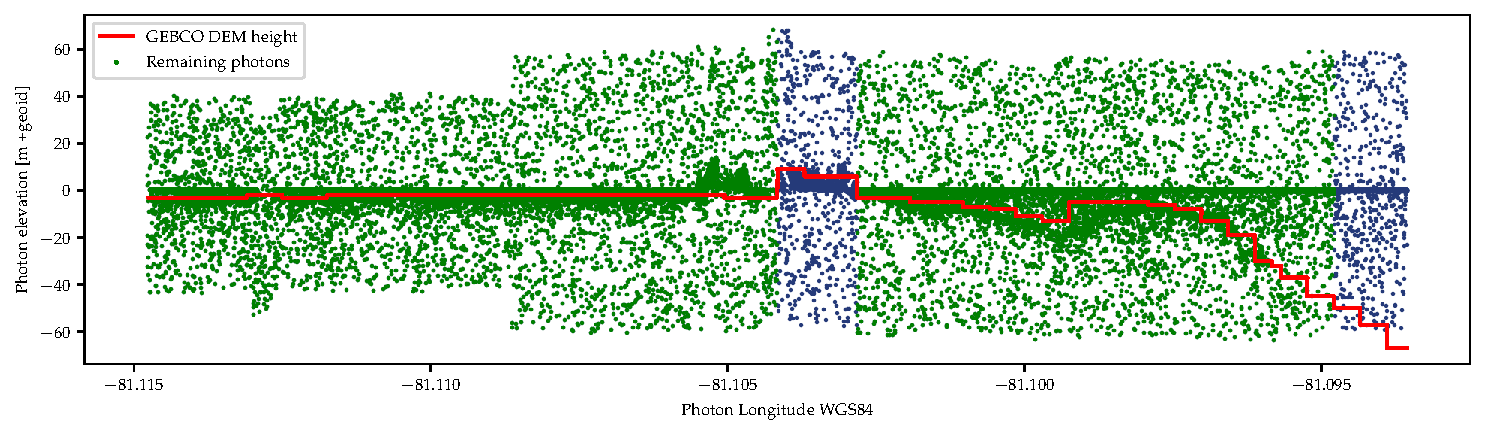
\includegraphics[width=\textwidth]{figures/methodology_gebco_filtering.jpg}
        \caption{The GEBCO data for the example transect, and the photons that are removed due to the GEBCO depth}
        \label{fig:gebco_filtering}
    \end{figure}

    \item To remove any high noise, cloud returns, or any remaining high land points not removed in step 1, any points more than 5m above the geoid are removed, based on the approach in \citeauthor{Ranndal2021}.
    \item The local sea-surface elevation $h_{sea}$ is calculated by taking the median elevation of photons that are classified as high-confidence sea surface photons. The water depth for each photon is then calculated. The standard deviation of the elevation high-confidence photons $\sigma_{h_{sea}}$ is also calculated to estimate the magnitude of the wave height at the time of the observation.
    \item Any points with a water depth greater than 40 meters, and points with an geoidal height  less than -40m are removed, based on the same assumption that they are too deep to by bathymetric points. 
    \item Any points that are higher than $h_{sea} + max(\sigma_{h_{sea}},1)$ are removed. 
    
    
    The results of steps 3-5 \pdfcomment{check} are shown in figure \ref{fig:vert_filtering}
    \pdfcomment{fix legend on this graph}
    \begin{figure}[h!]
        \centering
        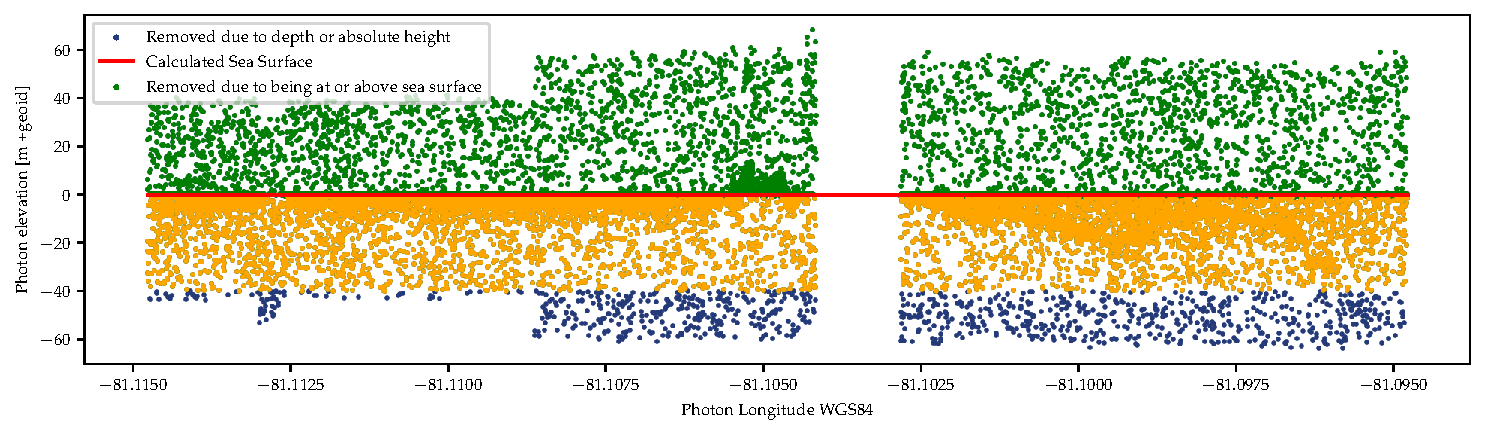
\includegraphics[width=\textwidth]{figures/methodology_sealvl_filtering.jpg}
        \caption{Vertical point filtering based on the local sea surface elevation}
        \label{fig:vert_filtering}
    \end{figure}
\end{enumerate}

After these filtering steps, the resulting subsurface photons for this example transect are shown in figure \ref{fig:remaing_photons}. The bathymetric signal can be seen clearly throughout the entire transect.

\begin{figure}[h!]
    \centering
    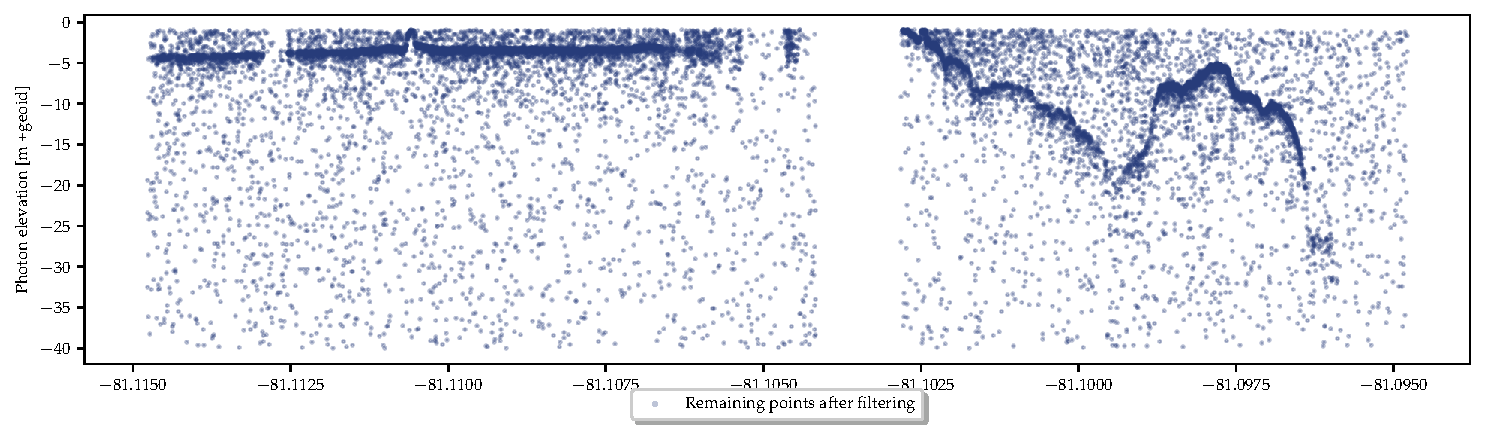
\includegraphics[width=\textwidth]{figures/methodology_reminaing_after_filtering.jpg}
    \caption{Subsurface photons found resulting after the filtering process}
    \label{fig:remaing_photons}
\end{figure}

An overview of the entire filtering chain is shown in figure \ref{fig:filtering-flowchart}

\begin{figure}[h!]
    \centering
    % %LaTeX with PSTricks extensions
%%Creator: Inkscape 1.2 (1:1.2.1+202207142221+cd75a1ee6d)
%%Please note this file requires PSTricks extensions
\psset{xunit=.5pt,yunit=.5pt,runit=.5pt}
\begin{pspicture}(791,1071)
{
\newrgbcolor{curcolor}{0 0 0}
\pscustom[linewidth=1,linecolor=curcolor]
{
\newpath
\moveto(313,1020.5)
\lineto(313,995.5)
\lineto(304,995.5)
\lineto(304,978.17)
}
}
{
\newrgbcolor{curcolor}{0 0 0}
\pscustom[linestyle=none,fillstyle=solid,fillcolor=curcolor]
{
\newpath
\moveto(304,972.92)
\lineto(300.5,979.92)
\lineto(304,978.17)
\lineto(307.5,979.92)
\closepath
}
}
{
\newrgbcolor{curcolor}{0 0 0}
\pscustom[linewidth=1,linecolor=curcolor]
{
\newpath
\moveto(304,972.92)
\lineto(300.5,979.92)
\lineto(304,978.17)
\lineto(307.5,979.92)
\closepath
}
}
{
\newrgbcolor{curcolor}{1 1 1}
\pscustom[linestyle=none,fillstyle=solid,fillcolor=curcolor]
{
\newpath
\moveto(140.5,1020.5)
\lineto(160.5,1070.5)
\lineto(370.5,1070.5)
\lineto(350.5,1020.5)
\closepath
}
}
{
\newrgbcolor{curcolor}{0 0 0}
\pscustom[linewidth=1,linecolor=curcolor]
{
\newpath
\moveto(140.5,1020.5)
\lineto(160.5,1070.5)
\lineto(370.5,1070.5)
\lineto(350.5,1020.5)
\closepath
}
}
{
\newrgbcolor{curcolor}{0 0 0}
\pscustom[linestyle=none,fillstyle=solid,fillcolor=curcolor]
{
\newpath
\moveto(223.44007901,1044.628)
\lineto(224.34007901,1042)
\lineto(225.58807901,1042)
\lineto(222.51607901,1050.748)
\lineto(221.07607901,1050.748)
\lineto(217.95607901,1042)
\lineto(219.14407901,1042)
\lineto(220.06807901,1044.628)
\closepath
\moveto(223.12807901,1045.564)
\lineto(220.34407901,1045.564)
\lineto(221.78407901,1049.548)
\closepath
}
}
{
\newrgbcolor{curcolor}{0 0 0}
\pscustom[linestyle=none,fillstyle=solid,fillcolor=curcolor]
{
\newpath
\moveto(228.88807187,1049.764)
\lineto(231.75607187,1049.764)
\lineto(231.75607187,1050.748)
\lineto(224.89207187,1050.748)
\lineto(224.89207187,1049.764)
\lineto(227.77207187,1049.764)
\lineto(227.77207187,1042)
\lineto(228.88807187,1042)
\closepath
}
}
{
\newrgbcolor{curcolor}{0 0 0}
\pscustom[linestyle=none,fillstyle=solid,fillcolor=curcolor]
{
\newpath
\moveto(233.90403726,1050.748)
\lineto(232.78803726,1050.748)
\lineto(232.78803726,1042)
\lineto(238.22403726,1042)
\lineto(238.22403726,1042.984)
\lineto(233.90403726,1042.984)
\closepath
}
}
{
\newrgbcolor{curcolor}{0 0 0}
\pscustom[linestyle=none,fillstyle=solid,fillcolor=curcolor]
{
\newpath
\moveto(241.80003433,1050.676)
\curveto(241.00803433,1050.676)(240.28803433,1050.316)(239.84403433,1049.728)
\curveto(239.29203433,1048.96)(239.01603433,1047.808)(239.01603433,1046.2)
\curveto(239.01603433,1043.272)(239.97603433,1041.724)(241.80003433,1041.724)
\curveto(243.60003433,1041.724)(244.58403433,1043.272)(244.58403433,1046.128)
\curveto(244.58403433,1047.808)(244.32003433,1048.936)(243.75603433,1049.728)
\curveto(243.31203433,1050.328)(242.60403433,1050.676)(241.80003433,1050.676)
\closepath
\moveto(241.80003433,1049.74)
\curveto(242.94003433,1049.74)(243.50403433,1048.576)(243.50403433,1046.224)
\curveto(243.50403433,1043.752)(242.95203433,1042.6)(241.77603433,1042.6)
\curveto(240.66003433,1042.6)(240.09603433,1043.8)(240.09603433,1046.188)
\curveto(240.09603433,1048.576)(240.66003433,1049.74)(241.80003433,1049.74)
\closepath
}
}
{
\newrgbcolor{curcolor}{0 0 0}
\pscustom[linestyle=none,fillstyle=solid,fillcolor=curcolor]
{
\newpath
\moveto(247.8240314,1045.996)
\lineto(247.9560314,1045.996)
\lineto(248.4000314,1045.996)
\curveto(249.5520314,1045.996)(250.1640314,1045.456)(250.1640314,1044.412)
\curveto(250.1640314,1043.32)(249.5040314,1042.66)(248.4120314,1042.66)
\curveto(247.2480314,1042.66)(246.6840314,1043.248)(246.6120314,1044.52)
\lineto(245.5560314,1044.52)
\curveto(245.6040314,1043.824)(245.7240314,1043.368)(245.9280314,1042.984)
\curveto(246.3720314,1042.144)(247.2000314,1041.724)(248.3640314,1041.724)
\curveto(250.1160314,1041.724)(251.2440314,1042.78)(251.2440314,1044.424)
\curveto(251.2440314,1045.528)(250.8240314,1046.128)(249.8040314,1046.488)
\curveto(250.5960314,1046.812)(250.9920314,1047.412)(250.9920314,1048.288)
\curveto(250.9920314,1049.776)(250.0200314,1050.676)(248.4000314,1050.676)
\curveto(246.6840314,1050.676)(245.7720314,1049.716)(245.7360314,1047.88)
\lineto(246.7920314,1047.88)
\curveto(246.8040314,1048.408)(246.8520314,1048.708)(246.9840314,1048.972)
\curveto(247.2240314,1049.464)(247.7520314,1049.752)(248.4120314,1049.752)
\curveto(249.3480314,1049.752)(249.9120314,1049.188)(249.9120314,1048.252)
\curveto(249.9120314,1047.64)(249.6960314,1047.268)(249.2280314,1047.064)
\curveto(248.9400314,1046.944)(248.5560314,1046.896)(247.8240314,1046.884)
\closepath
}
}
{
\newrgbcolor{curcolor}{0 0 0}
\pscustom[linestyle=none,fillstyle=solid,fillcolor=curcolor]
{
\newpath
\moveto(256.00802701,1048.288)
\lineto(256.00802701,1042)
\lineto(257.01602701,1042)
\lineto(257.01602701,1045.264)
\curveto(257.02802701,1046.776)(257.65202701,1047.448)(259.03202701,1047.412)
\lineto(259.03202701,1048.432)
\curveto(258.86402701,1048.456)(258.76802701,1048.468)(258.64802701,1048.468)
\curveto(258.00002701,1048.468)(257.50802701,1048.084)(256.93202701,1047.148)
\lineto(256.93202701,1048.288)
\closepath
}
}
{
\newrgbcolor{curcolor}{0 0 0}
\pscustom[linestyle=none,fillstyle=solid,fillcolor=curcolor]
{
\newpath
\moveto(265.21200357,1044.808)
\curveto(265.21200357,1045.768)(265.14000357,1046.344)(264.96000357,1046.812)
\curveto(264.55200357,1047.844)(263.59200357,1048.468)(262.41600357,1048.468)
\curveto(260.66400357,1048.468)(259.53600357,1047.136)(259.53600357,1045.06)
\curveto(259.53600357,1042.984)(260.61600357,1041.724)(262.39200357,1041.724)
\curveto(263.83200357,1041.724)(264.82800357,1042.54)(265.08000357,1043.908)
\lineto(264.07200357,1043.908)
\curveto(263.79600357,1043.08)(263.23200357,1042.648)(262.42800357,1042.648)
\curveto(261.79200357,1042.648)(261.25200357,1042.936)(260.91600357,1043.464)
\curveto(260.67600357,1043.824)(260.59200357,1044.184)(260.58000357,1044.808)
\closepath
\moveto(260.60400357,1045.624)
\curveto(260.68800357,1046.788)(261.39600357,1047.544)(262.40400357,1047.544)
\curveto(263.42400357,1047.544)(264.13200357,1046.752)(264.13200357,1045.624)
\closepath
}
}
{
\newrgbcolor{curcolor}{0 0 0}
\pscustom[linestyle=none,fillstyle=solid,fillcolor=curcolor]
{
\newpath
\moveto(268.6679913,1048.288)
\lineto(267.6359913,1048.288)
\lineto(267.6359913,1050.016)
\lineto(266.6399913,1050.016)
\lineto(266.6399913,1048.288)
\lineto(265.7879913,1048.288)
\lineto(265.7879913,1047.472)
\lineto(266.6399913,1047.472)
\lineto(266.6399913,1042.72)
\curveto(266.6399913,1042.072)(267.0719913,1041.724)(267.8519913,1041.724)
\curveto(268.1159913,1041.724)(268.3319913,1041.748)(268.6679913,1041.808)
\lineto(268.6679913,1042.648)
\curveto(268.5239913,1042.612)(268.3919913,1042.6)(268.1879913,1042.6)
\curveto(267.7559913,1042.6)(267.6359913,1042.72)(267.6359913,1043.164)
\lineto(267.6359913,1047.472)
\lineto(268.6679913,1047.472)
\closepath
}
}
{
\newrgbcolor{curcolor}{0 0 0}
\pscustom[linestyle=none,fillstyle=solid,fillcolor=curcolor]
{
\newpath
\moveto(274.69197043,1042)
\lineto(274.69197043,1048.288)
\lineto(273.69597043,1048.288)
\lineto(273.69597043,1044.724)
\curveto(273.69597043,1043.44)(273.02397043,1042.6)(271.97997043,1042.6)
\curveto(271.18797043,1042.6)(270.68397043,1043.08)(270.68397043,1043.836)
\lineto(270.68397043,1048.288)
\lineto(269.68797043,1048.288)
\lineto(269.68797043,1043.44)
\curveto(269.68797043,1042.396)(270.46797043,1041.724)(271.69197043,1041.724)
\curveto(272.61597043,1041.724)(273.20397043,1042.048)(273.79197043,1042.876)
\lineto(273.79197043,1042)
\closepath
}
}
{
\newrgbcolor{curcolor}{0 0 0}
\pscustom[linestyle=none,fillstyle=solid,fillcolor=curcolor]
{
\newpath
\moveto(276.4079675,1048.288)
\lineto(276.4079675,1042)
\lineto(277.4159675,1042)
\lineto(277.4159675,1045.264)
\curveto(277.4279675,1046.776)(278.0519675,1047.448)(279.4319675,1047.412)
\lineto(279.4319675,1048.432)
\curveto(279.2639675,1048.456)(279.1679675,1048.468)(279.0479675,1048.468)
\curveto(278.3999675,1048.468)(277.9079675,1048.084)(277.3319675,1047.148)
\lineto(277.3319675,1048.288)
\closepath
}
}
{
\newrgbcolor{curcolor}{0 0 0}
\pscustom[linestyle=none,fillstyle=solid,fillcolor=curcolor]
{
\newpath
\moveto(280.41594681,1048.288)
\lineto(280.41594681,1042)
\lineto(281.42394681,1042)
\lineto(281.42394681,1045.468)
\curveto(281.42394681,1046.752)(282.09594681,1047.592)(283.12794681,1047.592)
\curveto(283.91994681,1047.592)(284.42394681,1047.112)(284.42394681,1046.356)
\lineto(284.42394681,1042)
\lineto(285.41994681,1042)
\lineto(285.41994681,1046.752)
\curveto(285.41994681,1047.796)(284.63994681,1048.468)(283.42794681,1048.468)
\curveto(282.49194681,1048.468)(281.89194681,1048.108)(281.33994681,1047.232)
\lineto(281.33994681,1048.288)
\closepath
}
}
{
\newrgbcolor{curcolor}{0 0 0}
\pscustom[linestyle=none,fillstyle=solid,fillcolor=curcolor]
{
\newpath
\moveto(291.50394388,1046.536)
\curveto(291.49194388,1047.772)(290.67594388,1048.468)(289.22394388,1048.468)
\curveto(287.75994388,1048.468)(286.81194388,1047.712)(286.81194388,1046.548)
\curveto(286.81194388,1045.564)(287.31594388,1045.096)(288.80394388,1044.736)
\lineto(289.73994388,1044.508)
\curveto(290.43594388,1044.34)(290.71194388,1044.088)(290.71194388,1043.644)
\curveto(290.71194388,1043.044)(290.12394388,1042.648)(289.24794388,1042.648)
\curveto(288.70794388,1042.648)(288.25194388,1042.804)(287.99994388,1043.068)
\curveto(287.84394388,1043.248)(287.77194388,1043.428)(287.71194388,1043.872)
\lineto(286.65594388,1043.872)
\curveto(286.70394388,1042.42)(287.51994388,1041.724)(289.16394388,1041.724)
\curveto(290.74794388,1041.724)(291.75594388,1042.504)(291.75594388,1043.716)
\curveto(291.75594388,1044.652)(291.22794388,1045.168)(289.97994388,1045.468)
\lineto(289.01994388,1045.696)
\curveto(288.20394388,1045.888)(287.85594388,1046.152)(287.85594388,1046.596)
\curveto(287.85594388,1047.184)(288.37194388,1047.544)(289.18794388,1047.544)
\curveto(289.99194388,1047.544)(290.42394388,1047.196)(290.44794388,1046.536)
\closepath
}
}
{
\newrgbcolor{curcolor}{0 0 0}
\pscustom[linewidth=1,linecolor=curcolor]
{
\newpath
\moveto(370.5,840.5)
\lineto(370.5,820.5)
\lineto(190.5,820.5)
\lineto(190.5,806.87)
}
}
{
\newrgbcolor{curcolor}{0 0 0}
\pscustom[linestyle=none,fillstyle=solid,fillcolor=curcolor]
{
\newpath
\moveto(190.5,801.62)
\lineto(187,808.62)
\lineto(190.5,806.87)
\lineto(194,808.62)
\closepath
}
}
{
\newrgbcolor{curcolor}{0 0 0}
\pscustom[linewidth=1,linecolor=curcolor]
{
\newpath
\moveto(190.5,801.62)
\lineto(187,808.62)
\lineto(190.5,806.87)
\lineto(194,808.62)
\closepath
}
}
{
\newrgbcolor{curcolor}{1 1 1}
\pscustom[linestyle=none,fillstyle=solid,fillcolor=curcolor]
{
\newpath
\moveto(180.5,970.5)
\lineto(560.5,970.5)
\lineto(560.5,840.5)
\lineto(180.5,840.5)
\closepath
}
}
{
\newrgbcolor{curcolor}{0 0 0}
\pscustom[linewidth=1,linecolor=curcolor]
{
\newpath
\moveto(180.5,970.5)
\lineto(560.5,970.5)
\lineto(560.5,840.5)
\lineto(180.5,840.5)
\closepath
}
}
{
\newrgbcolor{curcolor}{0 0 0}
\pscustom[linestyle=none,fillstyle=solid,fillcolor=curcolor]
{
\newpath
\moveto(277.42616681,904.628)
\lineto(278.32616681,902)
\lineto(279.57416681,902)
\lineto(276.50216681,910.748)
\lineto(275.06216681,910.748)
\lineto(271.94216681,902)
\lineto(273.13016681,902)
\lineto(274.05416681,904.628)
\closepath
\moveto(277.11416681,905.564)
\lineto(274.33016681,905.564)
\lineto(275.77016681,909.548)
\closepath
}
}
{
\newrgbcolor{curcolor}{0 0 0}
\pscustom[linestyle=none,fillstyle=solid,fillcolor=curcolor]
{
\newpath
\moveto(284.9621615,906.536)
\curveto(284.9501615,907.772)(284.1341615,908.468)(282.6821615,908.468)
\curveto(281.2181615,908.468)(280.2701615,907.712)(280.2701615,906.548)
\curveto(280.2701615,905.564)(280.7741615,905.096)(282.2621615,904.736)
\lineto(283.1981615,904.508)
\curveto(283.8941615,904.34)(284.1701615,904.088)(284.1701615,903.644)
\curveto(284.1701615,903.044)(283.5821615,902.648)(282.7061615,902.648)
\curveto(282.1661615,902.648)(281.7101615,902.804)(281.4581615,903.068)
\curveto(281.3021615,903.248)(281.2301615,903.428)(281.1701615,903.872)
\lineto(280.1141615,903.872)
\curveto(280.1621615,902.42)(280.9781615,901.724)(282.6221615,901.724)
\curveto(284.2061615,901.724)(285.2141615,902.504)(285.2141615,903.716)
\curveto(285.2141615,904.652)(284.6861615,905.168)(283.4381615,905.468)
\lineto(282.4781615,905.696)
\curveto(281.6621615,905.888)(281.3141615,906.152)(281.3141615,906.596)
\curveto(281.3141615,907.184)(281.8301615,907.544)(282.6461615,907.544)
\curveto(283.4501615,907.544)(283.8821615,907.196)(283.9061615,906.536)
\closepath
}
}
{
\newrgbcolor{curcolor}{0 0 0}
\pscustom[linestyle=none,fillstyle=solid,fillcolor=curcolor]
{
\newpath
\moveto(290.98612543,906.536)
\curveto(290.97412543,907.772)(290.15812543,908.468)(288.70612543,908.468)
\curveto(287.24212543,908.468)(286.29412543,907.712)(286.29412543,906.548)
\curveto(286.29412543,905.564)(286.79812543,905.096)(288.28612543,904.736)
\lineto(289.22212543,904.508)
\curveto(289.91812543,904.34)(290.19412543,904.088)(290.19412543,903.644)
\curveto(290.19412543,903.044)(289.60612543,902.648)(288.73012543,902.648)
\curveto(288.19012543,902.648)(287.73412543,902.804)(287.48212543,903.068)
\curveto(287.32612543,903.248)(287.25412543,903.428)(287.19412543,903.872)
\lineto(286.13812543,903.872)
\curveto(286.18612543,902.42)(287.00212543,901.724)(288.64612543,901.724)
\curveto(290.23012543,901.724)(291.23812543,902.504)(291.23812543,903.716)
\curveto(291.23812543,904.652)(290.71012543,905.168)(289.46212543,905.468)
\lineto(288.50212543,905.696)
\curveto(287.68612543,905.888)(287.33812543,906.152)(287.33812543,906.596)
\curveto(287.33812543,907.184)(287.85412543,907.544)(288.67012543,907.544)
\curveto(289.47412543,907.544)(289.90612543,907.196)(289.93012543,906.536)
\closepath
}
}
{
\newrgbcolor{curcolor}{0 0 0}
\pscustom[linestyle=none,fillstyle=solid,fillcolor=curcolor]
{
\newpath
\moveto(293.53010254,908.288)
\lineto(292.53410254,908.288)
\lineto(292.53410254,902)
\lineto(293.53010254,902)
\closepath
\moveto(293.53010254,910.748)
\lineto(292.52210254,910.748)
\lineto(292.52210254,909.488)
\lineto(293.53010254,909.488)
\closepath
}
}
{
\newrgbcolor{curcolor}{0 0 0}
\pscustom[linestyle=none,fillstyle=solid,fillcolor=curcolor]
{
\newpath
\moveto(299.23006482,908.288)
\lineto(299.23006482,907.376)
\curveto(298.72606482,908.132)(298.17406482,908.468)(297.38206482,908.468)
\curveto(295.85806482,908.468)(294.80206482,907.052)(294.80206482,905.036)
\curveto(294.80206482,903.98)(295.05406482,903.212)(295.59406482,902.576)
\curveto(296.06206482,902.024)(296.66206482,901.724)(297.31006482,901.724)
\curveto(298.06606482,901.724)(298.60606482,902.06)(299.13406482,902.852)
\lineto(299.13406482,902.528)
\curveto(299.13406482,900.848)(298.66606482,900.224)(297.41806482,900.224)
\curveto(296.56606482,900.224)(296.12206482,900.56)(296.02606482,901.28)
\lineto(295.00606482,901.28)
\curveto(295.10206482,900.116)(296.02606482,899.384)(297.39406482,899.384)
\curveto(298.31806482,899.384)(299.08606482,899.684)(299.49406482,900.188)
\curveto(299.97406482,900.776)(300.15406482,901.556)(300.15406482,903.032)
\lineto(300.15406482,908.288)
\closepath
\moveto(297.47806482,907.544)
\curveto(298.53406482,907.544)(299.13406482,906.656)(299.13406482,905.06)
\curveto(299.13406482,903.536)(298.52206482,902.648)(297.47806482,902.648)
\curveto(296.44606482,902.648)(295.84606482,903.548)(295.84606482,905.096)
\curveto(295.84606482,906.632)(296.44606482,907.544)(297.47806482,907.544)
\closepath
}
}
{
\newrgbcolor{curcolor}{0 0 0}
\pscustom[linestyle=none,fillstyle=solid,fillcolor=curcolor]
{
\newpath
\moveto(301.89406189,908.288)
\lineto(301.89406189,902)
\lineto(302.90206189,902)
\lineto(302.90206189,905.468)
\curveto(302.90206189,906.752)(303.57406189,907.592)(304.60606189,907.592)
\curveto(305.39806189,907.592)(305.90206189,907.112)(305.90206189,906.356)
\lineto(305.90206189,902)
\lineto(306.89806189,902)
\lineto(306.89806189,906.752)
\curveto(306.89806189,907.796)(306.11806189,908.468)(304.90606189,908.468)
\curveto(303.97006189,908.468)(303.37006189,908.108)(302.81806189,907.232)
\lineto(302.81806189,908.288)
\closepath
}
}
{
\newrgbcolor{curcolor}{0 0 0}
\pscustom[linestyle=none,fillstyle=solid,fillcolor=curcolor]
{
\newpath
\moveto(319.5700575,906.62)
\lineto(315.9220575,906.62)
\lineto(315.9220575,905.636)
\lineto(318.5860575,905.636)
\lineto(318.5860575,905.396)
\curveto(318.5860575,903.836)(317.4340575,902.708)(315.8380575,902.708)
\curveto(314.9500575,902.708)(314.1460575,903.032)(313.6300575,903.596)
\curveto(313.0540575,904.22)(312.7060575,905.264)(312.7060575,906.344)
\curveto(312.7060575,908.492)(313.9300575,909.908)(315.7780575,909.908)
\curveto(317.1100575,909.908)(318.0700575,909.224)(318.3100575,908.096)
\lineto(319.4500575,908.096)
\curveto(319.1380575,909.872)(317.7940575,910.892)(315.7900575,910.892)
\curveto(314.7220575,910.892)(313.8580575,910.616)(313.1740575,910.052)
\curveto(312.1540575,909.212)(311.5900575,907.856)(311.5900575,906.284)
\curveto(311.5900575,903.596)(313.2340575,901.724)(315.5980575,901.724)
\curveto(316.7860575,901.724)(317.7220575,902.168)(318.5860575,903.116)
\lineto(318.8620575,901.952)
\lineto(319.5700575,901.952)
\closepath
}
}
{
\newrgbcolor{curcolor}{0 0 0}
\pscustom[linestyle=none,fillstyle=solid,fillcolor=curcolor]
{
\newpath
\moveto(322.59405603,905.984)
\lineto(327.35805603,905.984)
\lineto(327.35805603,906.968)
\lineto(322.59405603,906.968)
\lineto(322.59405603,909.764)
\lineto(327.53805603,909.764)
\lineto(327.53805603,910.748)
\lineto(321.47805603,910.748)
\lineto(321.47805603,902)
\lineto(327.75405603,902)
\lineto(327.75405603,902.984)
\lineto(322.59405603,902.984)
\closepath
}
}
{
\newrgbcolor{curcolor}{0 0 0}
\pscustom[linestyle=none,fillstyle=solid,fillcolor=curcolor]
{
\newpath
\moveto(329.35005383,902)
\lineto(333.29805383,902)
\curveto(334.12605383,902)(334.73805383,902.228)(335.20605383,902.732)
\curveto(335.63805383,903.188)(335.87805383,903.812)(335.87805383,904.496)
\curveto(335.87805383,905.552)(335.39805383,906.188)(334.28205383,906.62)
\curveto(335.08605383,906.992)(335.49405383,907.628)(335.49405383,908.528)
\curveto(335.49405383,909.176)(335.25405383,909.728)(334.79805383,910.136)
\curveto(334.33005383,910.556)(333.74205383,910.748)(332.90205383,910.748)
\lineto(329.35005383,910.748)
\closepath
\moveto(330.46605383,906.98)
\lineto(330.46605383,909.764)
\lineto(332.62605383,909.764)
\curveto(333.25005383,909.764)(333.59805383,909.68)(333.89805383,909.452)
\curveto(334.21005383,909.212)(334.37805383,908.852)(334.37805383,908.372)
\curveto(334.37805383,907.892)(334.21005383,907.532)(333.89805383,907.292)
\curveto(333.59805383,907.064)(333.25005383,906.98)(332.62605383,906.98)
\closepath
\moveto(330.46605383,902.984)
\lineto(330.46605383,905.996)
\lineto(333.19005383,905.996)
\curveto(334.17405383,905.996)(334.76205383,905.432)(334.76205383,904.484)
\curveto(334.76205383,903.548)(334.17405383,902.984)(333.19005383,902.984)
\closepath
}
}
{
\newrgbcolor{curcolor}{0 0 0}
\pscustom[linestyle=none,fillstyle=solid,fillcolor=curcolor]
{
\newpath
\moveto(344.2420423,908.036)
\curveto(343.8940423,909.956)(342.7900423,910.892)(340.8700423,910.892)
\curveto(339.6940423,910.892)(338.7460423,910.52)(338.0980423,909.8)
\curveto(337.3060423,908.936)(336.8740423,907.688)(336.8740423,906.272)
\curveto(336.8740423,904.832)(337.3180423,903.596)(338.1340423,902.744)
\curveto(338.8180423,902.048)(339.6820423,901.724)(340.8220423,901.724)
\curveto(342.9580423,901.724)(344.1580423,902.876)(344.4220423,905.192)
\lineto(343.2700423,905.192)
\curveto(343.1740423,904.592)(343.0540423,904.184)(342.8740423,903.836)
\curveto(342.5140423,903.116)(341.7700423,902.708)(340.8340423,902.708)
\curveto(339.0940423,902.708)(337.9900423,904.1)(337.9900423,906.284)
\curveto(337.9900423,908.528)(339.0340423,909.908)(340.7380423,909.908)
\curveto(341.4460423,909.908)(342.1060423,909.704)(342.4660423,909.356)
\curveto(342.7900423,909.056)(342.9700423,908.696)(343.1020423,908.036)
\closepath
}
}
{
\newrgbcolor{curcolor}{0 0 0}
\pscustom[linestyle=none,fillstyle=solid,fillcolor=curcolor]
{
\newpath
\moveto(349.53400494,910.892)
\curveto(347.02600494,910.892)(345.32200494,909.044)(345.32200494,906.308)
\curveto(345.32200494,903.56)(347.01400494,901.724)(349.54600494,901.724)
\curveto(350.61400494,901.724)(351.55000494,902.048)(352.25800494,902.648)
\curveto(353.20600494,903.452)(353.77000494,904.808)(353.77000494,906.236)
\curveto(353.77000494,909.056)(352.10200494,910.892)(349.53400494,910.892)
\closepath
\moveto(349.53400494,909.908)
\curveto(351.43000494,909.908)(352.65400494,908.48)(352.65400494,906.26)
\curveto(352.65400494,904.148)(351.39400494,902.708)(349.54600494,902.708)
\curveto(347.67400494,902.708)(346.43800494,904.148)(346.43800494,906.308)
\curveto(346.43800494,908.468)(347.67400494,909.908)(349.53400494,909.908)
\closepath
}
}
{
\newrgbcolor{curcolor}{0 0 0}
\pscustom[linestyle=none,fillstyle=solid,fillcolor=curcolor]
{
\newpath
\moveto(360.95800201,902)
\lineto(363.37000201,908.288)
\lineto(362.24200201,908.288)
\lineto(360.46600201,903.188)
\lineto(358.78600201,908.288)
\lineto(357.65800201,908.288)
\lineto(359.86600201,902)
\closepath
}
}
{
\newrgbcolor{curcolor}{0 0 0}
\pscustom[linestyle=none,fillstyle=solid,fillcolor=curcolor]
{
\newpath
\moveto(369.75397675,902.588)
\curveto(369.64597675,902.564)(369.59797675,902.564)(369.53797675,902.564)
\curveto(369.18997675,902.564)(368.99797675,902.744)(368.99797675,903.056)
\lineto(368.99797675,906.752)
\curveto(368.99797675,907.868)(368.18197675,908.468)(366.63397675,908.468)
\curveto(365.70997675,908.468)(364.97797675,908.204)(364.54597675,907.736)
\curveto(364.25797675,907.412)(364.13797675,907.052)(364.11397675,906.428)
\lineto(365.12197675,906.428)
\curveto(365.20597675,907.196)(365.66197675,907.544)(366.59797675,907.544)
\curveto(367.50997675,907.544)(368.00197675,907.208)(368.00197675,906.608)
\lineto(368.00197675,906.344)
\curveto(367.98997675,905.912)(367.77397675,905.756)(366.95797675,905.648)
\curveto(365.54197675,905.468)(365.32597675,905.42)(364.94197675,905.264)
\curveto(364.20997675,904.952)(363.83797675,904.4)(363.83797675,903.584)
\curveto(363.83797675,902.444)(364.62997675,901.724)(365.90197675,901.724)
\curveto(366.69397675,901.724)(367.32997675,902)(368.03797675,902.648)
\curveto(368.10997675,902)(368.42197675,901.724)(369.06997675,901.724)
\curveto(369.28597675,901.724)(369.41797675,901.748)(369.75397675,901.832)
\closepath
\moveto(368.00197675,903.98)
\curveto(368.00197675,903.644)(367.90597675,903.44)(367.60597675,903.164)
\curveto(367.19797675,902.792)(366.70597675,902.6)(366.11797675,902.6)
\curveto(365.33797675,902.6)(364.88197675,902.972)(364.88197675,903.608)
\curveto(364.88197675,904.268)(365.31397675,904.604)(366.39397675,904.76)
\curveto(367.46197675,904.904)(367.66597675,904.952)(368.00197675,905.108)
\closepath
}
}
{
\newrgbcolor{curcolor}{0 0 0}
\pscustom[linestyle=none,fillstyle=solid,fillcolor=curcolor]
{
\newpath
\moveto(371.82997382,910.748)
\lineto(370.82197382,910.748)
\lineto(370.82197382,902)
\lineto(371.82997382,902)
\closepath
}
}
{
\newrgbcolor{curcolor}{0 0 0}
\pscustom[linestyle=none,fillstyle=solid,fillcolor=curcolor]
{
\newpath
\moveto(378.45395239,902)
\lineto(378.45395239,908.288)
\lineto(377.45795239,908.288)
\lineto(377.45795239,904.724)
\curveto(377.45795239,903.44)(376.78595239,902.6)(375.74195239,902.6)
\curveto(374.94995239,902.6)(374.44595239,903.08)(374.44595239,903.836)
\lineto(374.44595239,908.288)
\lineto(373.44995239,908.288)
\lineto(373.44995239,903.44)
\curveto(373.44995239,902.396)(374.22995239,901.724)(375.45395239,901.724)
\curveto(376.37795239,901.724)(376.96595239,902.048)(377.55395239,902.876)
\lineto(377.55395239,902)
\closepath
}
}
{
\newrgbcolor{curcolor}{0 0 0}
\pscustom[linestyle=none,fillstyle=solid,fillcolor=curcolor]
{
\newpath
\moveto(385.49794946,904.808)
\curveto(385.49794946,905.768)(385.42594946,906.344)(385.24594946,906.812)
\curveto(384.83794946,907.844)(383.87794946,908.468)(382.70194946,908.468)
\curveto(380.94994946,908.468)(379.82194946,907.136)(379.82194946,905.06)
\curveto(379.82194946,902.984)(380.90194946,901.724)(382.67794946,901.724)
\curveto(384.11794946,901.724)(385.11394946,902.54)(385.36594946,903.908)
\lineto(384.35794946,903.908)
\curveto(384.08194946,903.08)(383.51794946,902.648)(382.71394946,902.648)
\curveto(382.07794946,902.648)(381.53794946,902.936)(381.20194946,903.464)
\curveto(380.96194946,903.824)(380.87794946,904.184)(380.86594946,904.808)
\closepath
\moveto(380.88994946,905.624)
\curveto(380.97394946,906.788)(381.68194946,907.544)(382.68994946,907.544)
\curveto(383.70994946,907.544)(384.41794946,906.752)(384.41794946,905.624)
\closepath
}
}
{
\newrgbcolor{curcolor}{0 0 0}
\pscustom[linestyle=none,fillstyle=solid,fillcolor=curcolor]
{
\newpath
\moveto(392.39794507,908.288)
\lineto(391.36594507,908.288)
\lineto(391.36594507,910.016)
\lineto(390.36994507,910.016)
\lineto(390.36994507,908.288)
\lineto(389.51794507,908.288)
\lineto(389.51794507,907.472)
\lineto(390.36994507,907.472)
\lineto(390.36994507,902.72)
\curveto(390.36994507,902.072)(390.80194507,901.724)(391.58194507,901.724)
\curveto(391.84594507,901.724)(392.06194507,901.748)(392.39794507,901.808)
\lineto(392.39794507,902.648)
\curveto(392.25394507,902.612)(392.12194507,902.6)(391.91794507,902.6)
\curveto(391.48594507,902.6)(391.36594507,902.72)(391.36594507,903.164)
\lineto(391.36594507,907.472)
\lineto(392.39794507,907.472)
\closepath
}
}
{
\newrgbcolor{curcolor}{0 0 0}
\pscustom[linestyle=none,fillstyle=solid,fillcolor=curcolor]
{
\newpath
\moveto(395.80593115,908.468)
\curveto(394.02993115,908.468)(392.97393115,907.208)(392.97393115,905.096)
\curveto(392.97393115,902.972)(394.02993115,901.724)(395.81793115,901.724)
\curveto(397.59393115,901.724)(398.66193115,902.984)(398.66193115,905.048)
\curveto(398.66193115,907.232)(397.62993115,908.468)(395.80593115,908.468)
\closepath
\moveto(395.81793115,907.544)
\curveto(396.94593115,907.544)(397.61793115,906.62)(397.61793115,905.06)
\curveto(397.61793115,903.572)(396.92193115,902.648)(395.81793115,902.648)
\curveto(394.70193115,902.648)(394.01793115,903.572)(394.01793115,905.096)
\curveto(394.01793115,906.62)(394.70193115,907.544)(395.81793115,907.544)
\closepath
}
}
{
\newrgbcolor{curcolor}{0 0 0}
\pscustom[linestyle=none,fillstyle=solid,fillcolor=curcolor]
{
\newpath
\moveto(408.70593439,904.808)
\curveto(408.70593439,905.768)(408.63393439,906.344)(408.45393439,906.812)
\curveto(408.04593439,907.844)(407.08593439,908.468)(405.90993439,908.468)
\curveto(404.15793439,908.468)(403.02993439,907.136)(403.02993439,905.06)
\curveto(403.02993439,902.984)(404.10993439,901.724)(405.88593439,901.724)
\curveto(407.32593439,901.724)(408.32193439,902.54)(408.57393439,903.908)
\lineto(407.56593439,903.908)
\curveto(407.28993439,903.08)(406.72593439,902.648)(405.92193439,902.648)
\curveto(405.28593439,902.648)(404.74593439,902.936)(404.40993439,903.464)
\curveto(404.16993439,903.824)(404.08593439,904.184)(404.07393439,904.808)
\closepath
\moveto(404.09793439,905.624)
\curveto(404.18193439,906.788)(404.88993439,907.544)(405.89793439,907.544)
\curveto(406.91793439,907.544)(407.62593439,906.752)(407.62593439,905.624)
\closepath
}
}
{
\newrgbcolor{curcolor}{0 0 0}
\pscustom[linestyle=none,fillstyle=solid,fillcolor=curcolor]
{
\newpath
\moveto(415.55790131,902.588)
\curveto(415.44990131,902.564)(415.40190131,902.564)(415.34190131,902.564)
\curveto(414.99390131,902.564)(414.80190131,902.744)(414.80190131,903.056)
\lineto(414.80190131,906.752)
\curveto(414.80190131,907.868)(413.98590131,908.468)(412.43790131,908.468)
\curveto(411.51390131,908.468)(410.78190131,908.204)(410.34990131,907.736)
\curveto(410.06190131,907.412)(409.94190131,907.052)(409.91790131,906.428)
\lineto(410.92590131,906.428)
\curveto(411.00990131,907.196)(411.46590131,907.544)(412.40190131,907.544)
\curveto(413.31390131,907.544)(413.80590131,907.208)(413.80590131,906.608)
\lineto(413.80590131,906.344)
\curveto(413.79390131,905.912)(413.57790131,905.756)(412.76190131,905.648)
\curveto(411.34590131,905.468)(411.12990131,905.42)(410.74590131,905.264)
\curveto(410.01390131,904.952)(409.64190131,904.4)(409.64190131,903.584)
\curveto(409.64190131,902.444)(410.43390131,901.724)(411.70590131,901.724)
\curveto(412.49790131,901.724)(413.13390131,902)(413.84190131,902.648)
\curveto(413.91390131,902)(414.22590131,901.724)(414.87390131,901.724)
\curveto(415.08990131,901.724)(415.22190131,901.748)(415.55790131,901.832)
\closepath
\moveto(413.80590131,903.98)
\curveto(413.80590131,903.644)(413.70990131,903.44)(413.40990131,903.164)
\curveto(413.00190131,902.792)(412.50990131,902.6)(411.92190131,902.6)
\curveto(411.14190131,902.6)(410.68590131,902.972)(410.68590131,903.608)
\curveto(410.68590131,904.268)(411.11790131,904.604)(412.19790131,904.76)
\curveto(413.26590131,904.904)(413.46990131,904.952)(413.80590131,905.108)
\closepath
}
}
{
\newrgbcolor{curcolor}{0 0 0}
\pscustom[linestyle=none,fillstyle=solid,fillcolor=curcolor]
{
\newpath
\moveto(421.46189838,906.176)
\curveto(421.41389838,906.788)(421.28189838,907.184)(421.04189838,907.532)
\curveto(420.60989838,908.12)(419.85389838,908.468)(418.97789838,908.468)
\curveto(417.27389838,908.468)(416.18189838,907.124)(416.18189838,905.036)
\curveto(416.18189838,903.008)(417.26189838,901.724)(418.96589838,901.724)
\curveto(420.46589838,901.724)(421.41389838,902.624)(421.53389838,904.16)
\lineto(420.52589838,904.16)
\curveto(420.35789838,903.152)(419.84189838,902.648)(418.98989838,902.648)
\curveto(417.88589838,902.648)(417.22589838,903.548)(417.22589838,905.036)
\curveto(417.22589838,906.608)(417.87389838,907.544)(418.96589838,907.544)
\curveto(419.80589838,907.544)(420.33389838,907.052)(420.45389838,906.176)
\closepath
}
}
{
\newrgbcolor{curcolor}{0 0 0}
\pscustom[linestyle=none,fillstyle=solid,fillcolor=curcolor]
{
\newpath
\moveto(422.64988312,910.748)
\lineto(422.64988312,902)
\lineto(423.64588312,902)
\lineto(423.64588312,905.468)
\curveto(423.64588312,906.752)(424.31788312,907.592)(425.34988312,907.592)
\curveto(425.68588312,907.592)(425.99788312,907.496)(426.23788312,907.316)
\curveto(426.52588312,907.1)(426.64588312,906.8)(426.64588312,906.356)
\lineto(426.64588312,902)
\lineto(427.64188312,902)
\lineto(427.64188312,906.752)
\curveto(427.64188312,907.808)(426.88588312,908.468)(425.66188312,908.468)
\curveto(424.77388312,908.468)(424.23388312,908.192)(423.64588312,907.424)
\lineto(423.64588312,910.748)
\closepath
}
}
{
\newrgbcolor{curcolor}{0 0 0}
\pscustom[linestyle=none,fillstyle=solid,fillcolor=curcolor]
{
\newpath
\moveto(432.46587872,899.384)
\lineto(433.47387872,899.384)
\lineto(433.47387872,902.66)
\curveto(434.00187872,902.012)(434.58987872,901.724)(435.40587872,901.724)
\curveto(437.03787872,901.724)(438.09387872,903.032)(438.09387872,905.036)
\curveto(438.09387872,907.148)(437.06187872,908.468)(435.39387872,908.468)
\curveto(434.54187872,908.468)(433.85787872,908.084)(433.38987872,907.34)
\lineto(433.38987872,908.288)
\lineto(432.46587872,908.288)
\closepath
\moveto(435.22587872,907.532)
\curveto(436.32987872,907.532)(437.04987872,906.56)(437.04987872,905.06)
\curveto(437.04987872,903.632)(436.31787872,902.66)(435.22587872,902.66)
\curveto(434.15787872,902.66)(433.47387872,903.62)(433.47387872,905.096)
\curveto(433.47387872,906.572)(434.15787872,907.532)(435.22587872,907.532)
\closepath
}
}
{
\newrgbcolor{curcolor}{0 0 0}
\pscustom[linestyle=none,fillstyle=solid,fillcolor=curcolor]
{
\newpath
\moveto(439.32987579,910.748)
\lineto(439.32987579,902)
\lineto(440.32587579,902)
\lineto(440.32587579,905.468)
\curveto(440.32587579,906.752)(440.99787579,907.592)(442.02987579,907.592)
\curveto(442.36587579,907.592)(442.67787579,907.496)(442.91787579,907.316)
\curveto(443.20587579,907.1)(443.32587579,906.8)(443.32587579,906.356)
\lineto(443.32587579,902)
\lineto(444.32187579,902)
\lineto(444.32187579,906.752)
\curveto(444.32187579,907.808)(443.56587579,908.468)(442.34187579,908.468)
\curveto(441.45387579,908.468)(440.91387579,908.192)(440.32587579,907.424)
\lineto(440.32587579,910.748)
\closepath
}
}
{
\newrgbcolor{curcolor}{0 0 0}
\pscustom[linestyle=none,fillstyle=solid,fillcolor=curcolor]
{
\newpath
\moveto(448.42587286,908.468)
\curveto(446.64987286,908.468)(445.59387286,907.208)(445.59387286,905.096)
\curveto(445.59387286,902.972)(446.64987286,901.724)(448.43787286,901.724)
\curveto(450.21387286,901.724)(451.28187286,902.984)(451.28187286,905.048)
\curveto(451.28187286,907.232)(450.24987286,908.468)(448.42587286,908.468)
\closepath
\moveto(448.43787286,907.544)
\curveto(449.56587286,907.544)(450.23787286,906.62)(450.23787286,905.06)
\curveto(450.23787286,903.572)(449.54187286,902.648)(448.43787286,902.648)
\curveto(447.32187286,902.648)(446.63787286,903.572)(446.63787286,905.096)
\curveto(446.63787286,906.62)(447.32187286,907.544)(448.43787286,907.544)
\closepath
}
}
{
\newrgbcolor{curcolor}{0 0 0}
\pscustom[linestyle=none,fillstyle=solid,fillcolor=curcolor]
{
\newpath
\moveto(454.77385297,908.288)
\lineto(453.74185297,908.288)
\lineto(453.74185297,910.016)
\lineto(452.74585297,910.016)
\lineto(452.74585297,908.288)
\lineto(451.89385297,908.288)
\lineto(451.89385297,907.472)
\lineto(452.74585297,907.472)
\lineto(452.74585297,902.72)
\curveto(452.74585297,902.072)(453.17785297,901.724)(453.95785297,901.724)
\curveto(454.22185297,901.724)(454.43785297,901.748)(454.77385297,901.808)
\lineto(454.77385297,902.648)
\curveto(454.62985297,902.612)(454.49785297,902.6)(454.29385297,902.6)
\curveto(453.86185297,902.6)(453.74185297,902.72)(453.74185297,903.164)
\lineto(453.74185297,907.472)
\lineto(454.77385297,907.472)
\closepath
}
}
{
\newrgbcolor{curcolor}{0 0 0}
\pscustom[linestyle=none,fillstyle=solid,fillcolor=curcolor]
{
\newpath
\moveto(458.18183905,908.468)
\curveto(456.40583905,908.468)(455.34983905,907.208)(455.34983905,905.096)
\curveto(455.34983905,902.972)(456.40583905,901.724)(458.19383905,901.724)
\curveto(459.96983905,901.724)(461.03783905,902.984)(461.03783905,905.048)
\curveto(461.03783905,907.232)(460.00583905,908.468)(458.18183905,908.468)
\closepath
\moveto(458.19383905,907.544)
\curveto(459.32183905,907.544)(459.99383905,906.62)(459.99383905,905.06)
\curveto(459.99383905,903.572)(459.29783905,902.648)(458.19383905,902.648)
\curveto(457.07783905,902.648)(456.39383905,903.572)(456.39383905,905.096)
\curveto(456.39383905,906.62)(457.07783905,907.544)(458.19383905,907.544)
\closepath
}
}
{
\newrgbcolor{curcolor}{0 0 0}
\pscustom[linestyle=none,fillstyle=solid,fillcolor=curcolor]
{
\newpath
\moveto(462.42983612,908.288)
\lineto(462.42983612,902)
\lineto(463.43783612,902)
\lineto(463.43783612,905.468)
\curveto(463.43783612,906.752)(464.10983612,907.592)(465.14183612,907.592)
\curveto(465.93383612,907.592)(466.43783612,907.112)(466.43783612,906.356)
\lineto(466.43783612,902)
\lineto(467.43383612,902)
\lineto(467.43383612,906.752)
\curveto(467.43383612,907.796)(466.65383612,908.468)(465.44183612,908.468)
\curveto(464.50583612,908.468)(463.90583612,908.108)(463.35383612,907.232)
\lineto(463.35383612,908.288)
\closepath
}
}
{
\newrgbcolor{curcolor}{0 0 0}
\pscustom[linewidth=1,linecolor=curcolor]
{
\newpath
\moveto(484.25,1020.5)
\lineto(484.3,995.5)
\lineto(495.9,995.5)
\lineto(495.9,981.81)
}
}
{
\newrgbcolor{curcolor}{0 0 0}
\pscustom[linestyle=none,fillstyle=solid,fillcolor=curcolor]
{
\newpath
\moveto(495.9,976.56)
\lineto(492.4,983.56)
\lineto(495.9,981.81)
\lineto(499.4,983.56)
\closepath
}
}
{
\newrgbcolor{curcolor}{0 0 0}
\pscustom[linewidth=1,linecolor=curcolor]
{
\newpath
\moveto(495.9,976.56)
\lineto(492.4,983.56)
\lineto(495.9,981.81)
\lineto(499.4,983.56)
\closepath
}
}
{
\newrgbcolor{curcolor}{1 1 1}
\pscustom[linestyle=none,fillstyle=solid,fillcolor=curcolor]
{
\newpath
\moveto(440.5,1020.5)
\lineto(460.5,1070.5)
\lineto(615.5,1070.5)
\lineto(595.5,1020.5)
\closepath
}
}
{
\newrgbcolor{curcolor}{0 0 0}
\pscustom[linewidth=1,linecolor=curcolor]
{
\newpath
\moveto(440.5,1020.5)
\lineto(460.5,1070.5)
\lineto(615.5,1070.5)
\lineto(595.5,1020.5)
\closepath
}
}
{
\newrgbcolor{curcolor}{0 0 0}
\pscustom[linestyle=none,fillstyle=solid,fillcolor=curcolor]
{
\newpath
\moveto(488.29207288,1046.62)
\lineto(484.64407288,1046.62)
\lineto(484.64407288,1045.636)
\lineto(487.30807288,1045.636)
\lineto(487.30807288,1045.396)
\curveto(487.30807288,1043.836)(486.15607288,1042.708)(484.56007288,1042.708)
\curveto(483.67207288,1042.708)(482.86807288,1043.032)(482.35207288,1043.596)
\curveto(481.77607288,1044.22)(481.42807288,1045.264)(481.42807288,1046.344)
\curveto(481.42807288,1048.492)(482.65207288,1049.908)(484.50007288,1049.908)
\curveto(485.83207288,1049.908)(486.79207288,1049.224)(487.03207288,1048.096)
\lineto(488.17207288,1048.096)
\curveto(487.86007288,1049.872)(486.51607288,1050.892)(484.51207288,1050.892)
\curveto(483.44407288,1050.892)(482.58007288,1050.616)(481.89607288,1050.052)
\curveto(480.87607288,1049.212)(480.31207288,1047.856)(480.31207288,1046.284)
\curveto(480.31207288,1043.596)(481.95607288,1041.724)(484.32007288,1041.724)
\curveto(485.50807288,1041.724)(486.44407288,1042.168)(487.30807288,1043.116)
\lineto(487.58407288,1041.952)
\lineto(488.29207288,1041.952)
\closepath
}
}
{
\newrgbcolor{curcolor}{0 0 0}
\pscustom[linestyle=none,fillstyle=solid,fillcolor=curcolor]
{
\newpath
\moveto(491.31607141,1045.984)
\lineto(496.08007141,1045.984)
\lineto(496.08007141,1046.968)
\lineto(491.31607141,1046.968)
\lineto(491.31607141,1049.764)
\lineto(496.26007141,1049.764)
\lineto(496.26007141,1050.748)
\lineto(490.20007141,1050.748)
\lineto(490.20007141,1042)
\lineto(496.47607141,1042)
\lineto(496.47607141,1042.984)
\lineto(491.31607141,1042.984)
\closepath
}
}
{
\newrgbcolor{curcolor}{0 0 0}
\pscustom[linestyle=none,fillstyle=solid,fillcolor=curcolor]
{
\newpath
\moveto(498.07206921,1042)
\lineto(502.02006921,1042)
\curveto(502.84806921,1042)(503.46006921,1042.228)(503.92806921,1042.732)
\curveto(504.36006921,1043.188)(504.60006921,1043.812)(504.60006921,1044.496)
\curveto(504.60006921,1045.552)(504.12006921,1046.188)(503.00406921,1046.62)
\curveto(503.80806921,1046.992)(504.21606921,1047.628)(504.21606921,1048.528)
\curveto(504.21606921,1049.176)(503.97606921,1049.728)(503.52006921,1050.136)
\curveto(503.05206921,1050.556)(502.46406921,1050.748)(501.62406921,1050.748)
\lineto(498.07206921,1050.748)
\closepath
\moveto(499.18806921,1046.98)
\lineto(499.18806921,1049.764)
\lineto(501.34806921,1049.764)
\curveto(501.97206921,1049.764)(502.32006921,1049.68)(502.62006921,1049.452)
\curveto(502.93206921,1049.212)(503.10006921,1048.852)(503.10006921,1048.372)
\curveto(503.10006921,1047.892)(502.93206921,1047.532)(502.62006921,1047.292)
\curveto(502.32006921,1047.064)(501.97206921,1046.98)(501.34806921,1046.98)
\closepath
\moveto(499.18806921,1042.984)
\lineto(499.18806921,1045.996)
\lineto(501.91206921,1045.996)
\curveto(502.89606921,1045.996)(503.48406921,1045.432)(503.48406921,1044.484)
\curveto(503.48406921,1043.548)(502.89606921,1042.984)(501.91206921,1042.984)
\closepath
}
}
{
\newrgbcolor{curcolor}{0 0 0}
\pscustom[linestyle=none,fillstyle=solid,fillcolor=curcolor]
{
\newpath
\moveto(512.96405768,1048.036)
\curveto(512.61605768,1049.956)(511.51205768,1050.892)(509.59205768,1050.892)
\curveto(508.41605768,1050.892)(507.46805768,1050.52)(506.82005768,1049.8)
\curveto(506.02805768,1048.936)(505.59605768,1047.688)(505.59605768,1046.272)
\curveto(505.59605768,1044.832)(506.04005768,1043.596)(506.85605768,1042.744)
\curveto(507.54005768,1042.048)(508.40405768,1041.724)(509.54405768,1041.724)
\curveto(511.68005768,1041.724)(512.88005768,1042.876)(513.14405768,1045.192)
\lineto(511.99205768,1045.192)
\curveto(511.89605768,1044.592)(511.77605768,1044.184)(511.59605768,1043.836)
\curveto(511.23605768,1043.116)(510.49205768,1042.708)(509.55605768,1042.708)
\curveto(507.81605768,1042.708)(506.71205768,1044.1)(506.71205768,1046.284)
\curveto(506.71205768,1048.528)(507.75605768,1049.908)(509.46005768,1049.908)
\curveto(510.16805768,1049.908)(510.82805768,1049.704)(511.18805768,1049.356)
\curveto(511.51205768,1049.056)(511.69205768,1048.696)(511.82405768,1048.036)
\closepath
}
}
{
\newrgbcolor{curcolor}{0 0 0}
\pscustom[linestyle=none,fillstyle=solid,fillcolor=curcolor]
{
\newpath
\moveto(518.25602032,1050.892)
\curveto(515.74802032,1050.892)(514.04402032,1049.044)(514.04402032,1046.308)
\curveto(514.04402032,1043.56)(515.73602032,1041.724)(518.26802032,1041.724)
\curveto(519.33602032,1041.724)(520.27202032,1042.048)(520.98002032,1042.648)
\curveto(521.92802032,1043.452)(522.49202032,1044.808)(522.49202032,1046.236)
\curveto(522.49202032,1049.056)(520.82402032,1050.892)(518.25602032,1050.892)
\closepath
\moveto(518.25602032,1049.908)
\curveto(520.15202032,1049.908)(521.37602032,1048.48)(521.37602032,1046.26)
\curveto(521.37602032,1044.148)(520.11602032,1042.708)(518.26802032,1042.708)
\curveto(516.39602032,1042.708)(515.16002032,1044.148)(515.16002032,1046.308)
\curveto(515.16002032,1048.468)(516.39602032,1049.908)(518.25602032,1049.908)
\closepath
}
}
{
\newrgbcolor{curcolor}{0 0 0}
\pscustom[linestyle=none,fillstyle=solid,fillcolor=curcolor]
{
\newpath
\moveto(532.3320174,1043.044)
\lineto(527.8560174,1043.044)
\curveto(527.9640174,1043.764)(528.3480174,1044.22)(529.3920174,1044.856)
\lineto(530.5920174,1045.528)
\curveto(531.7800174,1046.188)(532.3920174,1047.076)(532.3920174,1048.144)
\curveto(532.3920174,1048.864)(532.1040174,1049.536)(531.6000174,1050.004)
\curveto(531.0960174,1050.46)(530.4720174,1050.676)(529.6680174,1050.676)
\curveto(528.5880174,1050.676)(527.7840174,1050.292)(527.3160174,1049.548)
\curveto(527.0160174,1049.092)(526.8840174,1048.552)(526.8600174,1047.676)
\lineto(527.9160174,1047.676)
\curveto(527.9520174,1048.264)(528.0240174,1048.612)(528.1680174,1048.9)
\curveto(528.4440174,1049.428)(528.9960174,1049.752)(529.6320174,1049.752)
\curveto(530.5920174,1049.752)(531.3120174,1049.056)(531.3120174,1048.12)
\curveto(531.3120174,1047.424)(530.9160174,1046.824)(530.1600174,1046.392)
\lineto(529.0560174,1045.744)
\curveto(527.2800174,1044.724)(526.7640174,1043.908)(526.6680174,1042.012)
\lineto(532.3320174,1042.012)
\closepath
}
}
{
\newrgbcolor{curcolor}{0 0 0}
\pscustom[linestyle=none,fillstyle=solid,fillcolor=curcolor]
{
\newpath
\moveto(536.23201447,1050.676)
\curveto(535.44001447,1050.676)(534.72001447,1050.316)(534.27601447,1049.728)
\curveto(533.72401447,1048.96)(533.44801447,1047.808)(533.44801447,1046.2)
\curveto(533.44801447,1043.272)(534.40801447,1041.724)(536.23201447,1041.724)
\curveto(538.03201447,1041.724)(539.01601447,1043.272)(539.01601447,1046.128)
\curveto(539.01601447,1047.808)(538.75201447,1048.936)(538.18801447,1049.728)
\curveto(537.74401447,1050.328)(537.03601447,1050.676)(536.23201447,1050.676)
\closepath
\moveto(536.23201447,1049.74)
\curveto(537.37201447,1049.74)(537.93601447,1048.576)(537.93601447,1046.224)
\curveto(537.93601447,1043.752)(537.38401447,1042.6)(536.20801447,1042.6)
\curveto(535.09201447,1042.6)(534.52801447,1043.8)(534.52801447,1046.188)
\curveto(534.52801447,1048.576)(535.09201447,1049.74)(536.23201447,1049.74)
\closepath
}
}
{
\newrgbcolor{curcolor}{0 0 0}
\pscustom[linestyle=none,fillstyle=solid,fillcolor=curcolor]
{
\newpath
\moveto(545.67601154,1043.044)
\lineto(541.20001154,1043.044)
\curveto(541.30801154,1043.764)(541.69201154,1044.22)(542.73601154,1044.856)
\lineto(543.93601154,1045.528)
\curveto(545.12401154,1046.188)(545.73601154,1047.076)(545.73601154,1048.144)
\curveto(545.73601154,1048.864)(545.44801154,1049.536)(544.94401154,1050.004)
\curveto(544.44001154,1050.46)(543.81601154,1050.676)(543.01201154,1050.676)
\curveto(541.93201154,1050.676)(541.12801154,1050.292)(540.66001154,1049.548)
\curveto(540.36001154,1049.092)(540.22801154,1048.552)(540.20401154,1047.676)
\lineto(541.26001154,1047.676)
\curveto(541.29601154,1048.264)(541.36801154,1048.612)(541.51201154,1048.9)
\curveto(541.78801154,1049.428)(542.34001154,1049.752)(542.97601154,1049.752)
\curveto(543.93601154,1049.752)(544.65601154,1049.056)(544.65601154,1048.12)
\curveto(544.65601154,1047.424)(544.26001154,1046.824)(543.50401154,1046.392)
\lineto(542.40001154,1045.744)
\curveto(540.62401154,1044.724)(540.10801154,1043.908)(540.01201154,1042.012)
\lineto(545.67601154,1042.012)
\closepath
}
}
{
\newrgbcolor{curcolor}{0 0 0}
\pscustom[linestyle=none,fillstyle=solid,fillcolor=curcolor]
{
\newpath
\moveto(549.38400861,1048.18)
\lineto(549.38400861,1042)
\lineto(550.44000861,1042)
\lineto(550.44000861,1050.676)
\lineto(549.74400861,1050.676)
\curveto(549.37200861,1049.344)(549.13200861,1049.164)(547.50000861,1048.948)
\lineto(547.50000861,1048.18)
\closepath
}
}
{
\newrgbcolor{curcolor}{0 0 0}
\pscustom[linestyle=none,fillstyle=solid,fillcolor=curcolor]
{
\newpath
\moveto(561.13200421,1048.288)
\lineto(561.13200421,1047.376)
\curveto(560.62800421,1048.132)(560.07600421,1048.468)(559.28400421,1048.468)
\curveto(557.76000421,1048.468)(556.70400421,1047.052)(556.70400421,1045.036)
\curveto(556.70400421,1043.98)(556.95600421,1043.212)(557.49600421,1042.576)
\curveto(557.96400421,1042.024)(558.56400421,1041.724)(559.21200421,1041.724)
\curveto(559.96800421,1041.724)(560.50800421,1042.06)(561.03600421,1042.852)
\lineto(561.03600421,1042.528)
\curveto(561.03600421,1040.848)(560.56800421,1040.224)(559.32000421,1040.224)
\curveto(558.46800421,1040.224)(558.02400421,1040.56)(557.92800421,1041.28)
\lineto(556.90800421,1041.28)
\curveto(557.00400421,1040.116)(557.92800421,1039.384)(559.29600421,1039.384)
\curveto(560.22000421,1039.384)(560.98800421,1039.684)(561.39600421,1040.188)
\curveto(561.87600421,1040.776)(562.05600421,1041.556)(562.05600421,1043.032)
\lineto(562.05600421,1048.288)
\closepath
\moveto(559.38000421,1047.544)
\curveto(560.43600421,1047.544)(561.03600421,1046.656)(561.03600421,1045.06)
\curveto(561.03600421,1043.536)(560.42400421,1042.648)(559.38000421,1042.648)
\curveto(558.34800421,1042.648)(557.74800421,1043.548)(557.74800421,1045.096)
\curveto(557.74800421,1046.632)(558.34800421,1047.544)(559.38000421,1047.544)
\closepath
}
}
{
\newrgbcolor{curcolor}{0 0 0}
\pscustom[linestyle=none,fillstyle=solid,fillcolor=curcolor]
{
\newpath
\moveto(563.69997876,1048.288)
\lineto(563.69997876,1042)
\lineto(564.70797876,1042)
\lineto(564.70797876,1045.264)
\curveto(564.71997876,1046.776)(565.34397876,1047.448)(566.72397876,1047.412)
\lineto(566.72397876,1048.432)
\curveto(566.55597876,1048.456)(566.45997876,1048.468)(566.33997876,1048.468)
\curveto(565.69197876,1048.468)(565.19997876,1048.084)(564.62397876,1047.148)
\lineto(564.62397876,1048.288)
\closepath
}
}
{
\newrgbcolor{curcolor}{0 0 0}
\pscustom[linestyle=none,fillstyle=solid,fillcolor=curcolor]
{
\newpath
\moveto(568.67995148,1048.288)
\lineto(567.68395148,1048.288)
\lineto(567.68395148,1042)
\lineto(568.67995148,1042)
\closepath
\moveto(568.67995148,1050.748)
\lineto(567.67195148,1050.748)
\lineto(567.67195148,1049.488)
\lineto(568.67995148,1049.488)
\closepath
}
}
{
\newrgbcolor{curcolor}{0 0 0}
\pscustom[linestyle=none,fillstyle=solid,fillcolor=curcolor]
{
\newpath
\moveto(575.48393005,1050.748)
\lineto(574.48793005,1050.748)
\lineto(574.48793005,1047.496)
\curveto(574.06793005,1048.132)(573.39593005,1048.468)(572.55593005,1048.468)
\curveto(570.92393005,1048.468)(569.85593005,1047.16)(569.85593005,1045.156)
\curveto(569.85593005,1043.032)(570.88793005,1041.724)(572.59193005,1041.724)
\curveto(573.45593005,1041.724)(574.05593005,1042.048)(574.59593005,1042.828)
\lineto(574.59593005,1042)
\lineto(575.48393005,1042)
\closepath
\moveto(572.72393005,1047.532)
\curveto(573.80393005,1047.532)(574.48793005,1046.584)(574.48793005,1045.072)
\curveto(574.48793005,1043.62)(573.79193005,1042.66)(572.73593005,1042.66)
\curveto(571.63193005,1042.66)(570.89993005,1043.632)(570.89993005,1045.096)
\curveto(570.89993005,1046.56)(571.63193005,1047.532)(572.72393005,1047.532)
\closepath
}
}
{
\newrgbcolor{curcolor}{0 0 0}
\pscustom[linewidth=1,linecolor=curcolor]
{
\newpath
\moveto(380.5,700.5)
\lineto(400.5,700.5)
\lineto(390.5,700.5)
\lineto(404.13,700.5)
}
}
{
\newrgbcolor{curcolor}{0 0 0}
\pscustom[linestyle=none,fillstyle=solid,fillcolor=curcolor]
{
\newpath
\moveto(409.38,700.5)
\lineto(402.38,697)
\lineto(404.13,700.5)
\lineto(402.38,704)
\closepath
}
}
{
\newrgbcolor{curcolor}{0 0 0}
\pscustom[linewidth=1,linecolor=curcolor]
{
\newpath
\moveto(409.38,700.5)
\lineto(402.38,697)
\lineto(404.13,700.5)
\lineto(402.38,704)
\closepath
}
}
{
\newrgbcolor{curcolor}{1 1 1}
\pscustom[linestyle=none,fillstyle=solid,fillcolor=curcolor]
{
\newpath
\moveto(0.5,800.5)
\lineto(380.5,800.5)
\lineto(380.5,600.5)
\lineto(0.5,600.5)
\closepath
}
}
{
\newrgbcolor{curcolor}{0 0 0}
\pscustom[linewidth=1,linecolor=curcolor]
{
\newpath
\moveto(0.5,800.5)
\lineto(380.5,800.5)
\lineto(380.5,600.5)
\lineto(0.5,600.5)
\closepath
}
}
{
\newrgbcolor{curcolor}{0 0 0}
\pscustom[linestyle=none,fillstyle=solid,fillcolor=curcolor]
{
\newpath
\moveto(16.71430743,700.768)
\lineto(19.59430743,700.768)
\curveto(20.59030743,700.768)(21.03430743,700.288)(21.03430743,699.208)
\lineto(21.02230743,698.428)
\curveto(21.02230743,697.888)(21.11830743,697.36)(21.27430743,697)
\lineto(22.63030743,697)
\lineto(22.63030743,697.276)
\curveto(22.21030743,697.564)(22.12630743,697.876)(22.10230743,699.04)
\curveto(22.09030743,700.48)(21.86230743,700.912)(20.91430743,701.32)
\curveto(21.89830743,701.812)(22.29430743,702.4)(22.29430743,703.408)
\curveto(22.29430743,704.92)(21.35830743,705.748)(19.63030743,705.748)
\lineto(15.59830743,705.748)
\lineto(15.59830743,697)
\lineto(16.71430743,697)
\closepath
\moveto(16.71430743,701.752)
\lineto(16.71430743,704.764)
\lineto(19.41430743,704.764)
\curveto(20.03830743,704.764)(20.39830743,704.668)(20.67430743,704.428)
\curveto(20.97430743,704.176)(21.13030743,703.78)(21.13030743,703.264)
\curveto(21.13030743,702.22)(20.60230743,701.752)(19.41430743,701.752)
\closepath
}
}
{
\newrgbcolor{curcolor}{0 0 0}
\pscustom[linestyle=none,fillstyle=solid,fillcolor=curcolor]
{
\newpath
\moveto(29.18228326,699.808)
\curveto(29.18228326,700.768)(29.11028326,701.344)(28.93028326,701.812)
\curveto(28.52228326,702.844)(27.56228326,703.468)(26.38628326,703.468)
\curveto(24.63428326,703.468)(23.50628326,702.136)(23.50628326,700.06)
\curveto(23.50628326,697.984)(24.58628326,696.724)(26.36228326,696.724)
\curveto(27.80228326,696.724)(28.79828326,697.54)(29.05028326,698.908)
\lineto(28.04228326,698.908)
\curveto(27.76628326,698.08)(27.20228326,697.648)(26.39828326,697.648)
\curveto(25.76228326,697.648)(25.22228326,697.936)(24.88628326,698.464)
\curveto(24.64628326,698.824)(24.56228326,699.184)(24.55028326,699.808)
\closepath
\moveto(24.57428326,700.624)
\curveto(24.65828326,701.788)(25.36628326,702.544)(26.37428326,702.544)
\curveto(27.39428326,702.544)(28.10228326,701.752)(28.10228326,700.624)
\closepath
}
}
{
\newrgbcolor{curcolor}{0 0 0}
\pscustom[linestyle=none,fillstyle=solid,fillcolor=curcolor]
{
\newpath
\moveto(30.53828033,703.288)
\lineto(30.53828033,697)
\lineto(31.54628033,697)
\lineto(31.54628033,700.948)
\curveto(31.54628033,701.86)(32.20628033,702.592)(33.02228033,702.592)
\curveto(33.76628033,702.592)(34.18628033,702.136)(34.18628033,701.332)
\lineto(34.18628033,697)
\lineto(35.19428033,697)
\lineto(35.19428033,700.948)
\curveto(35.19428033,701.86)(35.85428033,702.592)(36.67028033,702.592)
\curveto(37.40228033,702.592)(37.83428033,702.124)(37.83428033,701.332)
\lineto(37.83428033,697)
\lineto(38.84228033,697)
\lineto(38.84228033,701.716)
\curveto(38.84228033,702.844)(38.19428033,703.468)(37.01828033,703.468)
\curveto(36.17828033,703.468)(35.67428033,703.216)(35.08628033,702.508)
\curveto(34.71428033,703.18)(34.21028033,703.468)(33.39428033,703.468)
\curveto(32.55428033,703.468)(31.99028033,703.156)(31.46228033,702.4)
\lineto(31.46228033,703.288)
\closepath
}
}
{
\newrgbcolor{curcolor}{0 0 0}
\pscustom[linestyle=none,fillstyle=solid,fillcolor=curcolor]
{
\newpath
\moveto(42.95825964,703.468)
\curveto(41.18225964,703.468)(40.12625964,702.208)(40.12625964,700.096)
\curveto(40.12625964,697.972)(41.18225964,696.724)(42.97025964,696.724)
\curveto(44.74625964,696.724)(45.81425964,697.984)(45.81425964,700.048)
\curveto(45.81425964,702.232)(44.78225964,703.468)(42.95825964,703.468)
\closepath
\moveto(42.97025964,702.544)
\curveto(44.09825964,702.544)(44.77025964,701.62)(44.77025964,700.06)
\curveto(44.77025964,698.572)(44.07425964,697.648)(42.97025964,697.648)
\curveto(41.85425964,697.648)(41.17025964,698.572)(41.17025964,700.096)
\curveto(41.17025964,701.62)(41.85425964,702.544)(42.97025964,702.544)
\closepath
}
}
{
\newrgbcolor{curcolor}{0 0 0}
\pscustom[linestyle=none,fillstyle=solid,fillcolor=curcolor]
{
\newpath
\moveto(49.57023804,697)
\lineto(51.98223804,703.288)
\lineto(50.85423804,703.288)
\lineto(49.07823804,698.188)
\lineto(47.39823804,703.288)
\lineto(46.27023804,703.288)
\lineto(48.47823804,697)
\closepath
}
}
{
\newrgbcolor{curcolor}{0 0 0}
\pscustom[linestyle=none,fillstyle=solid,fillcolor=curcolor]
{
\newpath
\moveto(58.06620966,699.808)
\curveto(58.06620966,700.768)(57.99420966,701.344)(57.81420966,701.812)
\curveto(57.40620966,702.844)(56.44620966,703.468)(55.27020966,703.468)
\curveto(53.51820966,703.468)(52.39020966,702.136)(52.39020966,700.06)
\curveto(52.39020966,697.984)(53.47020966,696.724)(55.24620966,696.724)
\curveto(56.68620966,696.724)(57.68220966,697.54)(57.93420966,698.908)
\lineto(56.92620966,698.908)
\curveto(56.65020966,698.08)(56.08620966,697.648)(55.28220966,697.648)
\curveto(54.64620966,697.648)(54.10620966,697.936)(53.77020966,698.464)
\curveto(53.53020966,698.824)(53.44620966,699.184)(53.43420966,699.808)
\closepath
\moveto(53.45820966,700.624)
\curveto(53.54220966,701.788)(54.25020966,702.544)(55.25820966,702.544)
\curveto(56.27820966,702.544)(56.98620966,701.752)(56.98620966,700.624)
\closepath
}
}
{
\newrgbcolor{curcolor}{0 0 0}
\pscustom[linestyle=none,fillstyle=solid,fillcolor=curcolor]
{
\newpath
\moveto(62.56620526,694.384)
\lineto(63.57420526,694.384)
\lineto(63.57420526,697.66)
\curveto(64.10220526,697.012)(64.69020526,696.724)(65.50620526,696.724)
\curveto(67.13820526,696.724)(68.19420526,698.032)(68.19420526,700.036)
\curveto(68.19420526,702.148)(67.16220526,703.468)(65.49420526,703.468)
\curveto(64.64220526,703.468)(63.95820526,703.084)(63.49020526,702.34)
\lineto(63.49020526,703.288)
\lineto(62.56620526,703.288)
\closepath
\moveto(65.32620526,702.532)
\curveto(66.43020526,702.532)(67.15020526,701.56)(67.15020526,700.06)
\curveto(67.15020526,698.632)(66.41820526,697.66)(65.32620526,697.66)
\curveto(64.25820526,697.66)(63.57420526,698.62)(63.57420526,700.096)
\curveto(63.57420526,701.572)(64.25820526,702.532)(65.32620526,702.532)
\closepath
}
}
{
\newrgbcolor{curcolor}{0 0 0}
\pscustom[linestyle=none,fillstyle=solid,fillcolor=curcolor]
{
\newpath
\moveto(71.85420233,703.468)
\curveto(70.07820233,703.468)(69.02220233,702.208)(69.02220233,700.096)
\curveto(69.02220233,697.972)(70.07820233,696.724)(71.86620233,696.724)
\curveto(73.64220233,696.724)(74.71020233,697.984)(74.71020233,700.048)
\curveto(74.71020233,702.232)(73.67820233,703.468)(71.85420233,703.468)
\closepath
\moveto(71.86620233,702.544)
\curveto(72.99420233,702.544)(73.66620233,701.62)(73.66620233,700.06)
\curveto(73.66620233,698.572)(72.97020233,697.648)(71.86620233,697.648)
\curveto(70.75020233,697.648)(70.06620233,698.572)(70.06620233,700.096)
\curveto(70.06620233,701.62)(70.75020233,702.544)(71.86620233,702.544)
\closepath
}
}
{
\newrgbcolor{curcolor}{0 0 0}
\pscustom[linestyle=none,fillstyle=solid,fillcolor=curcolor]
{
\newpath
\moveto(77.0621994,703.288)
\lineto(76.0661994,703.288)
\lineto(76.0661994,697)
\lineto(77.0621994,697)
\closepath
\moveto(77.0621994,705.748)
\lineto(76.0541994,705.748)
\lineto(76.0541994,704.488)
\lineto(77.0621994,704.488)
\closepath
}
}
{
\newrgbcolor{curcolor}{0 0 0}
\pscustom[linestyle=none,fillstyle=solid,fillcolor=curcolor]
{
\newpath
\moveto(78.76617798,703.288)
\lineto(78.76617798,697)
\lineto(79.77417798,697)
\lineto(79.77417798,700.468)
\curveto(79.77417798,701.752)(80.44617798,702.592)(81.47817798,702.592)
\curveto(82.27017798,702.592)(82.77417798,702.112)(82.77417798,701.356)
\lineto(82.77417798,697)
\lineto(83.77017798,697)
\lineto(83.77017798,701.752)
\curveto(83.77017798,702.796)(82.99017798,703.468)(81.77817798,703.468)
\curveto(80.84217798,703.468)(80.24217798,703.108)(79.69017798,702.232)
\lineto(79.69017798,703.288)
\closepath
}
}
{
\newrgbcolor{curcolor}{0 0 0}
\pscustom[linestyle=none,fillstyle=solid,fillcolor=curcolor]
{
\newpath
\moveto(87.64617505,703.288)
\lineto(86.61417505,703.288)
\lineto(86.61417505,705.016)
\lineto(85.61817505,705.016)
\lineto(85.61817505,703.288)
\lineto(84.76617505,703.288)
\lineto(84.76617505,702.472)
\lineto(85.61817505,702.472)
\lineto(85.61817505,697.72)
\curveto(85.61817505,697.072)(86.05017505,696.724)(86.83017505,696.724)
\curveto(87.09417505,696.724)(87.31017505,696.748)(87.64617505,696.808)
\lineto(87.64617505,697.648)
\curveto(87.50217505,697.612)(87.37017505,697.6)(87.16617505,697.6)
\curveto(86.73417505,697.6)(86.61417505,697.72)(86.61417505,698.164)
\lineto(86.61417505,702.472)
\lineto(87.64617505,702.472)
\closepath
}
}
{
\newrgbcolor{curcolor}{0 0 0}
\pscustom[linestyle=none,fillstyle=solid,fillcolor=curcolor]
{
\newpath
\moveto(93.19017358,701.536)
\curveto(93.17817358,702.772)(92.36217358,703.468)(90.91017358,703.468)
\curveto(89.44617358,703.468)(88.49817358,702.712)(88.49817358,701.548)
\curveto(88.49817358,700.564)(89.00217358,700.096)(90.49017358,699.736)
\lineto(91.42617358,699.508)
\curveto(92.12217358,699.34)(92.39817358,699.088)(92.39817358,698.644)
\curveto(92.39817358,698.044)(91.81017358,697.648)(90.93417358,697.648)
\curveto(90.39417358,697.648)(89.93817358,697.804)(89.68617358,698.068)
\curveto(89.53017358,698.248)(89.45817358,698.428)(89.39817358,698.872)
\lineto(88.34217358,698.872)
\curveto(88.39017358,697.42)(89.20617358,696.724)(90.85017358,696.724)
\curveto(92.43417358,696.724)(93.44217358,697.504)(93.44217358,698.716)
\curveto(93.44217358,699.652)(92.91417358,700.168)(91.66617358,700.468)
\lineto(90.70617358,700.696)
\curveto(89.89017358,700.888)(89.54217358,701.152)(89.54217358,701.596)
\curveto(89.54217358,702.184)(90.05817358,702.544)(90.87417358,702.544)
\curveto(91.67817358,702.544)(92.11017358,702.196)(92.13417358,701.536)
\closepath
}
}
{
\newrgbcolor{curcolor}{0 0 0}
\pscustom[linestyle=none,fillstyle=solid,fillcolor=curcolor]
{
\newpath
\moveto(100.36614923,703.288)
\lineto(99.32214923,703.288)
\lineto(99.32214923,704.272)
\curveto(99.32214923,704.692)(99.55014923,704.908)(100.01814923,704.908)
\curveto(100.10214923,704.908)(100.13814923,704.908)(100.36614923,704.896)
\lineto(100.36614923,705.724)
\curveto(100.13814923,705.772)(100.00614923,705.784)(99.80214923,705.784)
\curveto(98.87814923,705.784)(98.32614923,705.256)(98.32614923,704.356)
\lineto(98.32614923,703.288)
\lineto(97.48614923,703.288)
\lineto(97.48614923,702.472)
\lineto(98.32614923,702.472)
\lineto(98.32614923,697)
\lineto(99.32214923,697)
\lineto(99.32214923,702.472)
\lineto(100.36614923,702.472)
\closepath
}
}
{
\newrgbcolor{curcolor}{0 0 0}
\pscustom[linestyle=none,fillstyle=solid,fillcolor=curcolor]
{
\newpath
\moveto(101.43414777,703.288)
\lineto(101.43414777,697)
\lineto(102.44214777,697)
\lineto(102.44214777,700.264)
\curveto(102.45414777,701.776)(103.07814777,702.448)(104.45814777,702.412)
\lineto(104.45814777,703.432)
\curveto(104.29014777,703.456)(104.19414777,703.468)(104.07414777,703.468)
\curveto(103.42614777,703.468)(102.93414777,703.084)(102.35814777,702.148)
\lineto(102.35814777,703.288)
\closepath
}
}
{
\newrgbcolor{curcolor}{0 0 0}
\pscustom[linestyle=none,fillstyle=solid,fillcolor=curcolor]
{
\newpath
\moveto(107.79412085,703.468)
\curveto(106.01812085,703.468)(104.96212085,702.208)(104.96212085,700.096)
\curveto(104.96212085,697.972)(106.01812085,696.724)(107.80612085,696.724)
\curveto(109.58212085,696.724)(110.65012085,697.984)(110.65012085,700.048)
\curveto(110.65012085,702.232)(109.61812085,703.468)(107.79412085,703.468)
\closepath
\moveto(107.80612085,702.544)
\curveto(108.93412085,702.544)(109.60612085,701.62)(109.60612085,700.06)
\curveto(109.60612085,698.572)(108.91012085,697.648)(107.80612085,697.648)
\curveto(106.69012085,697.648)(106.00612085,698.572)(106.00612085,700.096)
\curveto(106.00612085,701.62)(106.69012085,702.544)(107.80612085,702.544)
\closepath
}
}
{
\newrgbcolor{curcolor}{0 0 0}
\pscustom[linestyle=none,fillstyle=solid,fillcolor=curcolor]
{
\newpath
\moveto(112.04211792,703.288)
\lineto(112.04211792,697)
\lineto(113.05011792,697)
\lineto(113.05011792,700.948)
\curveto(113.05011792,701.86)(113.71011792,702.592)(114.52611792,702.592)
\curveto(115.27011792,702.592)(115.69011792,702.136)(115.69011792,701.332)
\lineto(115.69011792,697)
\lineto(116.69811792,697)
\lineto(116.69811792,700.948)
\curveto(116.69811792,701.86)(117.35811792,702.592)(118.17411792,702.592)
\curveto(118.90611792,702.592)(119.33811792,702.124)(119.33811792,701.332)
\lineto(119.33811792,697)
\lineto(120.34611792,697)
\lineto(120.34611792,701.716)
\curveto(120.34611792,702.844)(119.69811792,703.468)(118.52211792,703.468)
\curveto(117.68211792,703.468)(117.17811792,703.216)(116.59011792,702.508)
\curveto(116.21811792,703.18)(115.71411792,703.468)(114.89811792,703.468)
\curveto(114.05811792,703.468)(113.49411792,703.156)(112.96611792,702.4)
\lineto(112.96611792,703.288)
\closepath
}
}
{
\newrgbcolor{curcolor}{0 0 0}
\pscustom[linestyle=none,fillstyle=solid,fillcolor=curcolor]
{
\newpath
\moveto(129.85009576,703.288)
\lineto(125.15809576,703.288)
\lineto(125.15809576,702.412)
\lineto(128.66209576,702.412)
\lineto(124.90609576,697.9)
\lineto(124.90609576,697)
\lineto(130.01809576,697)
\lineto(130.01809576,697.876)
\lineto(126.11809576,697.876)
\lineto(129.85009576,702.4)
\closepath
}
}
{
\newrgbcolor{curcolor}{0 0 0}
\pscustom[linestyle=none,fillstyle=solid,fillcolor=curcolor]
{
\newpath
\moveto(133.54605109,703.468)
\curveto(131.77005109,703.468)(130.71405109,702.208)(130.71405109,700.096)
\curveto(130.71405109,697.972)(131.77005109,696.724)(133.55805109,696.724)
\curveto(135.33405109,696.724)(136.40205109,697.984)(136.40205109,700.048)
\curveto(136.40205109,702.232)(135.37005109,703.468)(133.54605109,703.468)
\closepath
\moveto(133.55805109,702.544)
\curveto(134.68605109,702.544)(135.35805109,701.62)(135.35805109,700.06)
\curveto(135.35805109,698.572)(134.66205109,697.648)(133.55805109,697.648)
\curveto(132.44205109,697.648)(131.75805109,698.572)(131.75805109,700.096)
\curveto(131.75805109,701.62)(132.44205109,702.544)(133.55805109,702.544)
\closepath
}
}
{
\newrgbcolor{curcolor}{0 0 0}
\pscustom[linestyle=none,fillstyle=solid,fillcolor=curcolor]
{
\newpath
\moveto(137.79404816,703.288)
\lineto(137.79404816,697)
\lineto(138.80204816,697)
\lineto(138.80204816,700.468)
\curveto(138.80204816,701.752)(139.47404816,702.592)(140.50604816,702.592)
\curveto(141.29804816,702.592)(141.80204816,702.112)(141.80204816,701.356)
\lineto(141.80204816,697)
\lineto(142.79804816,697)
\lineto(142.79804816,701.752)
\curveto(142.79804816,702.796)(142.01804816,703.468)(140.80604816,703.468)
\curveto(139.87004816,703.468)(139.27004816,703.108)(138.71804816,702.232)
\lineto(138.71804816,703.288)
\closepath
}
}
{
\newrgbcolor{curcolor}{0 0 0}
\pscustom[linestyle=none,fillstyle=solid,fillcolor=curcolor]
{
\newpath
\moveto(149.78204523,699.808)
\curveto(149.78204523,700.768)(149.71004523,701.344)(149.53004523,701.812)
\curveto(149.12204523,702.844)(148.16204523,703.468)(146.98604523,703.468)
\curveto(145.23404523,703.468)(144.10604523,702.136)(144.10604523,700.06)
\curveto(144.10604523,697.984)(145.18604523,696.724)(146.96204523,696.724)
\curveto(148.40204523,696.724)(149.39804523,697.54)(149.65004523,698.908)
\lineto(148.64204523,698.908)
\curveto(148.36604523,698.08)(147.80204523,697.648)(146.99804523,697.648)
\curveto(146.36204523,697.648)(145.82204523,697.936)(145.48604523,698.464)
\curveto(145.24604523,698.824)(145.16204523,699.184)(145.15004523,699.808)
\closepath
\moveto(145.17404523,700.624)
\curveto(145.25804523,701.788)(145.96604523,702.544)(146.97404523,702.544)
\curveto(147.99404523,702.544)(148.70204523,701.752)(148.70204523,700.624)
\closepath
}
}
{
\newrgbcolor{curcolor}{0 0 0}
\pscustom[linestyle=none,fillstyle=solid,fillcolor=curcolor]
{
\newpath
\moveto(155.50602289,701.536)
\curveto(155.49402289,702.772)(154.67802289,703.468)(153.22602289,703.468)
\curveto(151.76202289,703.468)(150.81402289,702.712)(150.81402289,701.548)
\curveto(150.81402289,700.564)(151.31802289,700.096)(152.80602289,699.736)
\lineto(153.74202289,699.508)
\curveto(154.43802289,699.34)(154.71402289,699.088)(154.71402289,698.644)
\curveto(154.71402289,698.044)(154.12602289,697.648)(153.25002289,697.648)
\curveto(152.71002289,697.648)(152.25402289,697.804)(152.00202289,698.068)
\curveto(151.84602289,698.248)(151.77402289,698.428)(151.71402289,698.872)
\lineto(150.65802289,698.872)
\curveto(150.70602289,697.42)(151.52202289,696.724)(153.16602289,696.724)
\curveto(154.75002289,696.724)(155.75802289,697.504)(155.75802289,698.716)
\curveto(155.75802289,699.652)(155.23002289,700.168)(153.98202289,700.468)
\lineto(153.02202289,700.696)
\curveto(152.20602289,700.888)(151.85802289,701.152)(151.85802289,701.596)
\curveto(151.85802289,702.184)(152.37402289,702.544)(153.19002289,702.544)
\curveto(153.99402289,702.544)(154.42602289,702.196)(154.45002289,701.536)
\closepath
}
}
{
\newrgbcolor{curcolor}{0 0 0}
\pscustom[linestyle=none,fillstyle=solid,fillcolor=curcolor]
{
\newpath
\moveto(162.63400616,703.288)
\lineto(161.60200616,703.288)
\lineto(161.60200616,705.016)
\lineto(160.60600616,705.016)
\lineto(160.60600616,703.288)
\lineto(159.75400616,703.288)
\lineto(159.75400616,702.472)
\lineto(160.60600616,702.472)
\lineto(160.60600616,697.72)
\curveto(160.60600616,697.072)(161.03800616,696.724)(161.81800616,696.724)
\curveto(162.08200616,696.724)(162.29800616,696.748)(162.63400616,696.808)
\lineto(162.63400616,697.648)
\curveto(162.49000616,697.612)(162.35800616,697.6)(162.15400616,697.6)
\curveto(161.72200616,697.6)(161.60200616,697.72)(161.60200616,698.164)
\lineto(161.60200616,702.472)
\lineto(162.63400616,702.472)
\closepath
}
}
{
\newrgbcolor{curcolor}{0 0 0}
\pscustom[linestyle=none,fillstyle=solid,fillcolor=curcolor]
{
\newpath
\moveto(163.68998322,705.748)
\lineto(163.68998322,697)
\lineto(164.68598322,697)
\lineto(164.68598322,700.468)
\curveto(164.68598322,701.752)(165.35798322,702.592)(166.38998322,702.592)
\curveto(166.72598322,702.592)(167.03798322,702.496)(167.27798322,702.316)
\curveto(167.56598322,702.1)(167.68598322,701.8)(167.68598322,701.356)
\lineto(167.68598322,697)
\lineto(168.68198322,697)
\lineto(168.68198322,701.752)
\curveto(168.68198322,702.808)(167.92598322,703.468)(166.70198322,703.468)
\curveto(165.81398322,703.468)(165.27398322,703.192)(164.68598322,702.424)
\lineto(164.68598322,705.748)
\closepath
}
}
{
\newrgbcolor{curcolor}{0 0 0}
\pscustom[linestyle=none,fillstyle=solid,fillcolor=curcolor]
{
\newpath
\moveto(175.94198029,697.588)
\curveto(175.83398029,697.564)(175.78598029,697.564)(175.72598029,697.564)
\curveto(175.37798029,697.564)(175.18598029,697.744)(175.18598029,698.056)
\lineto(175.18598029,701.752)
\curveto(175.18598029,702.868)(174.36998029,703.468)(172.82198029,703.468)
\curveto(171.89798029,703.468)(171.16598029,703.204)(170.73398029,702.736)
\curveto(170.44598029,702.412)(170.32598029,702.052)(170.30198029,701.428)
\lineto(171.30998029,701.428)
\curveto(171.39398029,702.196)(171.84998029,702.544)(172.78598029,702.544)
\curveto(173.69798029,702.544)(174.18998029,702.208)(174.18998029,701.608)
\lineto(174.18998029,701.344)
\curveto(174.17798029,700.912)(173.96198029,700.756)(173.14598029,700.648)
\curveto(171.72998029,700.468)(171.51398029,700.42)(171.12998029,700.264)
\curveto(170.39798029,699.952)(170.02598029,699.4)(170.02598029,698.584)
\curveto(170.02598029,697.444)(170.81798029,696.724)(172.08998029,696.724)
\curveto(172.88198029,696.724)(173.51798029,697)(174.22598029,697.648)
\curveto(174.29798029,697)(174.60998029,696.724)(175.25798029,696.724)
\curveto(175.47398029,696.724)(175.60598029,696.748)(175.94198029,696.832)
\closepath
\moveto(174.18998029,698.98)
\curveto(174.18998029,698.644)(174.09398029,698.44)(173.79398029,698.164)
\curveto(173.38598029,697.792)(172.89398029,697.6)(172.30598029,697.6)
\curveto(171.52598029,697.6)(171.06998029,697.972)(171.06998029,698.608)
\curveto(171.06998029,699.268)(171.50198029,699.604)(172.58198029,699.76)
\curveto(173.64998029,699.904)(173.85398029,699.952)(174.18998029,700.108)
\closepath
}
}
{
\newrgbcolor{curcolor}{0 0 0}
\pscustom[linestyle=none,fillstyle=solid,fillcolor=curcolor]
{
\newpath
\moveto(179.10995831,703.288)
\lineto(178.07795831,703.288)
\lineto(178.07795831,705.016)
\lineto(177.08195831,705.016)
\lineto(177.08195831,703.288)
\lineto(176.22995831,703.288)
\lineto(176.22995831,702.472)
\lineto(177.08195831,702.472)
\lineto(177.08195831,697.72)
\curveto(177.08195831,697.072)(177.51395831,696.724)(178.29395831,696.724)
\curveto(178.55795831,696.724)(178.77395831,696.748)(179.10995831,696.808)
\lineto(179.10995831,697.648)
\curveto(178.96595831,697.612)(178.83395831,697.6)(178.62995831,697.6)
\curveto(178.19795831,697.6)(178.07795831,697.72)(178.07795831,698.164)
\lineto(178.07795831,702.472)
\lineto(179.10995831,702.472)
\closepath
}
}
{
\newrgbcolor{curcolor}{0 0 0}
\pscustom[linestyle=none,fillstyle=solid,fillcolor=curcolor]
{
\newpath
\moveto(189.15395538,697.588)
\curveto(189.04595538,697.564)(188.99795538,697.564)(188.93795538,697.564)
\curveto(188.58995538,697.564)(188.39795538,697.744)(188.39795538,698.056)
\lineto(188.39795538,701.752)
\curveto(188.39795538,702.868)(187.58195538,703.468)(186.03395538,703.468)
\curveto(185.10995538,703.468)(184.37795538,703.204)(183.94595538,702.736)
\curveto(183.65795538,702.412)(183.53795538,702.052)(183.51395538,701.428)
\lineto(184.52195538,701.428)
\curveto(184.60595538,702.196)(185.06195538,702.544)(185.99795538,702.544)
\curveto(186.90995538,702.544)(187.40195538,702.208)(187.40195538,701.608)
\lineto(187.40195538,701.344)
\curveto(187.38995538,700.912)(187.17395538,700.756)(186.35795538,700.648)
\curveto(184.94195538,700.468)(184.72595538,700.42)(184.34195538,700.264)
\curveto(183.60995538,699.952)(183.23795538,699.4)(183.23795538,698.584)
\curveto(183.23795538,697.444)(184.02995538,696.724)(185.30195538,696.724)
\curveto(186.09395538,696.724)(186.72995538,697)(187.43795538,697.648)
\curveto(187.50995538,697)(187.82195538,696.724)(188.46995538,696.724)
\curveto(188.68595538,696.724)(188.81795538,696.748)(189.15395538,696.832)
\closepath
\moveto(187.40195538,698.98)
\curveto(187.40195538,698.644)(187.30595538,698.44)(187.00595538,698.164)
\curveto(186.59795538,697.792)(186.10595538,697.6)(185.51795538,697.6)
\curveto(184.73795538,697.6)(184.28195538,697.972)(184.28195538,698.608)
\curveto(184.28195538,699.268)(184.71395538,699.604)(185.79395538,699.76)
\curveto(186.86195538,699.904)(187.06595538,699.952)(187.40195538,700.108)
\closepath
}
}
{
\newrgbcolor{curcolor}{0 0 0}
\pscustom[linestyle=none,fillstyle=solid,fillcolor=curcolor]
{
\newpath
\moveto(190.23395245,703.288)
\lineto(190.23395245,697)
\lineto(191.24195245,697)
\lineto(191.24195245,700.264)
\curveto(191.25395245,701.776)(191.87795245,702.448)(193.25795245,702.412)
\lineto(193.25795245,703.432)
\curveto(193.08995245,703.456)(192.99395245,703.468)(192.87395245,703.468)
\curveto(192.22595245,703.468)(191.73395245,703.084)(191.15795245,702.148)
\lineto(191.15795245,703.288)
\closepath
}
}
{
\newrgbcolor{curcolor}{0 0 0}
\pscustom[linestyle=none,fillstyle=solid,fillcolor=curcolor]
{
\newpath
\moveto(199.43792902,699.808)
\curveto(199.43792902,700.768)(199.36592902,701.344)(199.18592902,701.812)
\curveto(198.77792902,702.844)(197.81792902,703.468)(196.64192902,703.468)
\curveto(194.88992902,703.468)(193.76192902,702.136)(193.76192902,700.06)
\curveto(193.76192902,697.984)(194.84192902,696.724)(196.61792902,696.724)
\curveto(198.05792902,696.724)(199.05392902,697.54)(199.30592902,698.908)
\lineto(198.29792902,698.908)
\curveto(198.02192902,698.08)(197.45792902,697.648)(196.65392902,697.648)
\curveto(196.01792902,697.648)(195.47792902,697.936)(195.14192902,698.464)
\curveto(194.90192902,698.824)(194.81792902,699.184)(194.80592902,699.808)
\closepath
\moveto(194.82992902,700.624)
\curveto(194.91392902,701.788)(195.62192902,702.544)(196.62992902,702.544)
\curveto(197.64992902,702.544)(198.35792902,701.752)(198.35792902,700.624)
\closepath
}
}
{
\newrgbcolor{curcolor}{0 0 0}
\pscustom[linestyle=none,fillstyle=solid,fillcolor=curcolor]
{
\newpath
\moveto(206.33792462,703.288)
\lineto(205.30592462,703.288)
\lineto(205.30592462,705.016)
\lineto(204.30992462,705.016)
\lineto(204.30992462,703.288)
\lineto(203.45792462,703.288)
\lineto(203.45792462,702.472)
\lineto(204.30992462,702.472)
\lineto(204.30992462,697.72)
\curveto(204.30992462,697.072)(204.74192462,696.724)(205.52192462,696.724)
\curveto(205.78592462,696.724)(206.00192462,696.748)(206.33792462,696.808)
\lineto(206.33792462,697.648)
\curveto(206.19392462,697.612)(206.06192462,697.6)(205.85792462,697.6)
\curveto(205.42592462,697.6)(205.30592462,697.72)(205.30592462,698.164)
\lineto(205.30592462,702.472)
\lineto(206.33792462,702.472)
\closepath
}
}
{
\newrgbcolor{curcolor}{0 0 0}
\pscustom[linestyle=none,fillstyle=solid,fillcolor=curcolor]
{
\newpath
\moveto(209.74591071,703.468)
\curveto(207.96991071,703.468)(206.91391071,702.208)(206.91391071,700.096)
\curveto(206.91391071,697.972)(207.96991071,696.724)(209.75791071,696.724)
\curveto(211.53391071,696.724)(212.60191071,697.984)(212.60191071,700.048)
\curveto(212.60191071,702.232)(211.56991071,703.468)(209.74591071,703.468)
\closepath
\moveto(209.75791071,702.544)
\curveto(210.88591071,702.544)(211.55791071,701.62)(211.55791071,700.06)
\curveto(211.55791071,698.572)(210.86191071,697.648)(209.75791071,697.648)
\curveto(208.64191071,697.648)(207.95791071,698.572)(207.95791071,700.096)
\curveto(207.95791071,701.62)(208.64191071,702.544)(209.75791071,702.544)
\closepath
}
}
{
\newrgbcolor{curcolor}{0 0 0}
\pscustom[linestyle=none,fillstyle=solid,fillcolor=curcolor]
{
\newpath
\moveto(216.41790778,703.468)
\curveto(214.64190778,703.468)(213.58590778,702.208)(213.58590778,700.096)
\curveto(213.58590778,697.972)(214.64190778,696.724)(216.42990778,696.724)
\curveto(218.20590778,696.724)(219.27390778,697.984)(219.27390778,700.048)
\curveto(219.27390778,702.232)(218.24190778,703.468)(216.41790778,703.468)
\closepath
\moveto(216.42990778,702.544)
\curveto(217.55790778,702.544)(218.22990778,701.62)(218.22990778,700.06)
\curveto(218.22990778,698.572)(217.53390778,697.648)(216.42990778,697.648)
\curveto(215.31390778,697.648)(214.62990778,698.572)(214.62990778,700.096)
\curveto(214.62990778,701.62)(215.31390778,702.544)(216.42990778,702.544)
\closepath
}
}
{
\newrgbcolor{curcolor}{0 0 0}
\pscustom[linestyle=none,fillstyle=solid,fillcolor=curcolor]
{
\newpath
\moveto(229.10190338,705.748)
\lineto(228.10590338,705.748)
\lineto(228.10590338,702.496)
\curveto(227.68590338,703.132)(227.01390338,703.468)(226.17390338,703.468)
\curveto(224.54190338,703.468)(223.47390338,702.16)(223.47390338,700.156)
\curveto(223.47390338,698.032)(224.50590338,696.724)(226.20990338,696.724)
\curveto(227.07390338,696.724)(227.67390338,697.048)(228.21390338,697.828)
\lineto(228.21390338,697)
\lineto(229.10190338,697)
\closepath
\moveto(226.34190338,702.532)
\curveto(227.42190338,702.532)(228.10590338,701.584)(228.10590338,700.072)
\curveto(228.10590338,698.62)(227.40990338,697.66)(226.35390338,697.66)
\curveto(225.24990338,697.66)(224.51790338,698.632)(224.51790338,700.096)
\curveto(224.51790338,701.56)(225.24990338,702.532)(226.34190338,702.532)
\closepath
}
}
{
\newrgbcolor{curcolor}{0 0 0}
\pscustom[linestyle=none,fillstyle=solid,fillcolor=curcolor]
{
\newpath
\moveto(235.98990045,699.808)
\curveto(235.98990045,700.768)(235.91790045,701.344)(235.73790045,701.812)
\curveto(235.32990045,702.844)(234.36990045,703.468)(233.19390045,703.468)
\curveto(231.44190045,703.468)(230.31390045,702.136)(230.31390045,700.06)
\curveto(230.31390045,697.984)(231.39390045,696.724)(233.16990045,696.724)
\curveto(234.60990045,696.724)(235.60590045,697.54)(235.85790045,698.908)
\lineto(234.84990045,698.908)
\curveto(234.57390045,698.08)(234.00990045,697.648)(233.20590045,697.648)
\curveto(232.56990045,697.648)(232.02990045,697.936)(231.69390045,698.464)
\curveto(231.45390045,698.824)(231.36990045,699.184)(231.35790045,699.808)
\closepath
\moveto(231.38190045,700.624)
\curveto(231.46590045,701.788)(232.17390045,702.544)(233.18190045,702.544)
\curveto(234.20190045,702.544)(234.90990045,701.752)(234.90990045,700.624)
\closepath
}
}
{
\newrgbcolor{curcolor}{0 0 0}
\pscustom[linestyle=none,fillstyle=solid,fillcolor=curcolor]
{
\newpath
\moveto(242.66189752,699.808)
\curveto(242.66189752,700.768)(242.58989752,701.344)(242.40989752,701.812)
\curveto(242.00189752,702.844)(241.04189752,703.468)(239.86589752,703.468)
\curveto(238.11389752,703.468)(236.98589752,702.136)(236.98589752,700.06)
\curveto(236.98589752,697.984)(238.06589752,696.724)(239.84189752,696.724)
\curveto(241.28189752,696.724)(242.27789752,697.54)(242.52989752,698.908)
\lineto(241.52189752,698.908)
\curveto(241.24589752,698.08)(240.68189752,697.648)(239.87789752,697.648)
\curveto(239.24189752,697.648)(238.70189752,697.936)(238.36589752,698.464)
\curveto(238.12589752,698.824)(238.04189752,699.184)(238.02989752,699.808)
\closepath
\moveto(238.05389752,700.624)
\curveto(238.13789752,701.788)(238.84589752,702.544)(239.85389752,702.544)
\curveto(240.87389752,702.544)(241.58189752,701.752)(241.58189752,700.624)
\closepath
}
}
{
\newrgbcolor{curcolor}{0 0 0}
\pscustom[linestyle=none,fillstyle=solid,fillcolor=curcolor]
{
\newpath
\moveto(243.82589459,694.384)
\lineto(244.83389459,694.384)
\lineto(244.83389459,697.66)
\curveto(245.36189459,697.012)(245.94989459,696.724)(246.76589459,696.724)
\curveto(248.39789459,696.724)(249.45389459,698.032)(249.45389459,700.036)
\curveto(249.45389459,702.148)(248.42189459,703.468)(246.75389459,703.468)
\curveto(245.90189459,703.468)(245.21789459,703.084)(244.74989459,702.34)
\lineto(244.74989459,703.288)
\lineto(243.82589459,703.288)
\closepath
\moveto(246.58589459,702.532)
\curveto(247.68989459,702.532)(248.40989459,701.56)(248.40989459,700.06)
\curveto(248.40989459,698.632)(247.67789459,697.66)(246.58589459,697.66)
\curveto(245.51789459,697.66)(244.83389459,698.62)(244.83389459,700.096)
\curveto(244.83389459,701.572)(245.51789459,702.532)(246.58589459,702.532)
\closepath
}
}
{
\newrgbcolor{curcolor}{0 0 0}
\pscustom[linestyle=none,fillstyle=solid,fillcolor=curcolor]
{
\newpath
\moveto(256.4498902,703.468)
\curveto(254.6738902,703.468)(253.6178902,702.208)(253.6178902,700.096)
\curveto(253.6178902,697.972)(254.6738902,696.724)(256.4618902,696.724)
\curveto(258.2378902,696.724)(259.3058902,697.984)(259.3058902,700.048)
\curveto(259.3058902,702.232)(258.2738902,703.468)(256.4498902,703.468)
\closepath
\moveto(256.4618902,702.544)
\curveto(257.5898902,702.544)(258.2618902,701.62)(258.2618902,700.06)
\curveto(258.2618902,698.572)(257.5658902,697.648)(256.4618902,697.648)
\curveto(255.3458902,697.648)(254.6618902,698.572)(254.6618902,700.096)
\curveto(254.6618902,701.62)(255.3458902,702.544)(256.4618902,702.544)
\closepath
}
}
{
\newrgbcolor{curcolor}{0 0 0}
\pscustom[linestyle=none,fillstyle=solid,fillcolor=curcolor]
{
\newpath
\moveto(260.68588727,703.288)
\lineto(260.68588727,697)
\lineto(261.69388727,697)
\lineto(261.69388727,700.264)
\curveto(261.70588727,701.776)(262.32988727,702.448)(263.70988727,702.412)
\lineto(263.70988727,703.432)
\curveto(263.54188727,703.456)(263.44588727,703.468)(263.32588727,703.468)
\curveto(262.67788727,703.468)(262.18588727,703.084)(261.60988727,702.148)
\lineto(261.60988727,703.288)
\closepath
}
}
{
\newrgbcolor{curcolor}{0 0 0}
\pscustom[linestyle=none,fillstyle=solid,fillcolor=curcolor]
{
\newpath
\moveto(270.23787274,703.288)
\lineto(269.20587274,703.288)
\lineto(269.20587274,705.016)
\lineto(268.20987274,705.016)
\lineto(268.20987274,703.288)
\lineto(267.35787274,703.288)
\lineto(267.35787274,702.472)
\lineto(268.20987274,702.472)
\lineto(268.20987274,697.72)
\curveto(268.20987274,697.072)(268.64187274,696.724)(269.42187274,696.724)
\curveto(269.68587274,696.724)(269.90187274,696.748)(270.23787274,696.808)
\lineto(270.23787274,697.648)
\curveto(270.09387274,697.612)(269.96187274,697.6)(269.75787274,697.6)
\curveto(269.32587274,697.6)(269.20587274,697.72)(269.20587274,698.164)
\lineto(269.20587274,702.472)
\lineto(270.23787274,702.472)
\closepath
}
}
{
\newrgbcolor{curcolor}{0 0 0}
\pscustom[linestyle=none,fillstyle=solid,fillcolor=curcolor]
{
\newpath
\moveto(273.64585883,703.468)
\curveto(271.86985883,703.468)(270.81385883,702.208)(270.81385883,700.096)
\curveto(270.81385883,697.972)(271.86985883,696.724)(273.65785883,696.724)
\curveto(275.43385883,696.724)(276.50185883,697.984)(276.50185883,700.048)
\curveto(276.50185883,702.232)(275.46985883,703.468)(273.64585883,703.468)
\closepath
\moveto(273.65785883,702.544)
\curveto(274.78585883,702.544)(275.45785883,701.62)(275.45785883,700.06)
\curveto(275.45785883,698.572)(274.76185883,697.648)(273.65785883,697.648)
\curveto(272.54185883,697.648)(271.85785883,698.572)(271.85785883,700.096)
\curveto(271.85785883,701.62)(272.54185883,702.544)(273.65785883,702.544)
\closepath
}
}
{
\newrgbcolor{curcolor}{0 0 0}
\pscustom[linestyle=none,fillstyle=solid,fillcolor=curcolor]
{
\newpath
\moveto(280.31784064,703.468)
\curveto(278.54184064,703.468)(277.48584064,702.208)(277.48584064,700.096)
\curveto(277.48584064,697.972)(278.54184064,696.724)(280.32984064,696.724)
\curveto(282.10584064,696.724)(283.17384064,697.984)(283.17384064,700.048)
\curveto(283.17384064,702.232)(282.14184064,703.468)(280.31784064,703.468)
\closepath
\moveto(280.32984064,702.544)
\curveto(281.45784064,702.544)(282.12984064,701.62)(282.12984064,700.06)
\curveto(282.12984064,698.572)(281.43384064,697.648)(280.32984064,697.648)
\curveto(279.21384064,697.648)(278.52984064,698.572)(278.52984064,700.096)
\curveto(278.52984064,701.62)(279.21384064,702.544)(280.32984064,702.544)
\closepath
}
}
{
\newrgbcolor{curcolor}{0 0 0}
\pscustom[linestyle=none,fillstyle=solid,fillcolor=curcolor]
{
\newpath
\moveto(287.90183624,705.748)
\lineto(287.90183624,697)
\lineto(288.89783624,697)
\lineto(288.89783624,700.468)
\curveto(288.89783624,701.752)(289.56983624,702.592)(290.60183624,702.592)
\curveto(290.93783624,702.592)(291.24983624,702.496)(291.48983624,702.316)
\curveto(291.77783624,702.1)(291.89783624,701.8)(291.89783624,701.356)
\lineto(291.89783624,697)
\lineto(292.89383624,697)
\lineto(292.89383624,701.752)
\curveto(292.89383624,702.808)(292.13783624,703.468)(290.91383624,703.468)
\curveto(290.02583624,703.468)(289.48583624,703.192)(288.89783624,702.424)
\lineto(288.89783624,705.748)
\closepath
}
}
{
\newrgbcolor{curcolor}{0 0 0}
\pscustom[linestyle=none,fillstyle=solid,fillcolor=curcolor]
{
\newpath
\moveto(295.53383331,703.288)
\lineto(294.53783331,703.288)
\lineto(294.53783331,697)
\lineto(295.53383331,697)
\closepath
\moveto(295.53383331,705.748)
\lineto(294.52583331,705.748)
\lineto(294.52583331,704.488)
\lineto(295.53383331,704.488)
\closepath
}
}
{
\newrgbcolor{curcolor}{0 0 0}
\pscustom[linestyle=none,fillstyle=solid,fillcolor=curcolor]
{
\newpath
\moveto(301.23381085,703.288)
\lineto(301.23381085,702.376)
\curveto(300.72981085,703.132)(300.17781085,703.468)(299.38581085,703.468)
\curveto(297.86181085,703.468)(296.80581085,702.052)(296.80581085,700.036)
\curveto(296.80581085,698.98)(297.05781085,698.212)(297.59781085,697.576)
\curveto(298.06581085,697.024)(298.66581085,696.724)(299.31381085,696.724)
\curveto(300.06981085,696.724)(300.60981085,697.06)(301.13781085,697.852)
\lineto(301.13781085,697.528)
\curveto(301.13781085,695.848)(300.66981085,695.224)(299.42181085,695.224)
\curveto(298.56981085,695.224)(298.12581085,695.56)(298.02981085,696.28)
\lineto(297.00981085,696.28)
\curveto(297.10581085,695.116)(298.02981085,694.384)(299.39781085,694.384)
\curveto(300.32181085,694.384)(301.08981085,694.684)(301.49781085,695.188)
\curveto(301.97781085,695.776)(302.15781085,696.556)(302.15781085,698.032)
\lineto(302.15781085,703.288)
\closepath
\moveto(299.48181085,702.544)
\curveto(300.53781085,702.544)(301.13781085,701.656)(301.13781085,700.06)
\curveto(301.13781085,698.536)(300.52581085,697.648)(299.48181085,697.648)
\curveto(298.44981085,697.648)(297.84981085,698.548)(297.84981085,700.096)
\curveto(297.84981085,701.632)(298.44981085,702.544)(299.48181085,702.544)
\closepath
}
}
{
\newrgbcolor{curcolor}{0 0 0}
\pscustom[linestyle=none,fillstyle=solid,fillcolor=curcolor]
{
\newpath
\moveto(303.81379303,705.748)
\lineto(303.81379303,697)
\lineto(304.80979303,697)
\lineto(304.80979303,700.468)
\curveto(304.80979303,701.752)(305.48179303,702.592)(306.51379303,702.592)
\curveto(306.84979303,702.592)(307.16179303,702.496)(307.40179303,702.316)
\curveto(307.68979303,702.1)(307.80979303,701.8)(307.80979303,701.356)
\lineto(307.80979303,697)
\lineto(308.80579303,697)
\lineto(308.80579303,701.752)
\curveto(308.80579303,702.808)(308.04979303,703.468)(306.82579303,703.468)
\curveto(305.93779303,703.468)(305.39779303,703.192)(304.80979303,702.424)
\lineto(304.80979303,705.748)
\closepath
}
}
{
\newrgbcolor{curcolor}{0 0 0}
\pscustom[linestyle=none,fillstyle=solid,fillcolor=curcolor]
{
\newpath
\moveto(316.02978864,703.288)
\lineto(314.99778864,703.288)
\lineto(314.99778864,705.016)
\lineto(314.00178864,705.016)
\lineto(314.00178864,703.288)
\lineto(313.14978864,703.288)
\lineto(313.14978864,702.472)
\lineto(314.00178864,702.472)
\lineto(314.00178864,697.72)
\curveto(314.00178864,697.072)(314.43378864,696.724)(315.21378864,696.724)
\curveto(315.47778864,696.724)(315.69378864,696.748)(316.02978864,696.808)
\lineto(316.02978864,697.648)
\curveto(315.88578864,697.612)(315.75378864,697.6)(315.54978864,697.6)
\curveto(315.11778864,697.6)(314.99778864,697.72)(314.99778864,698.164)
\lineto(314.99778864,702.472)
\lineto(316.02978864,702.472)
\closepath
}
}
{
\newrgbcolor{curcolor}{0 0 0}
\pscustom[linestyle=none,fillstyle=solid,fillcolor=curcolor]
{
\newpath
\moveto(319.43777472,703.468)
\curveto(317.66177472,703.468)(316.60577472,702.208)(316.60577472,700.096)
\curveto(316.60577472,697.972)(317.66177472,696.724)(319.44977472,696.724)
\curveto(321.22577472,696.724)(322.29377472,697.984)(322.29377472,700.048)
\curveto(322.29377472,702.232)(321.26177472,703.468)(319.43777472,703.468)
\closepath
\moveto(319.44977472,702.544)
\curveto(320.57777472,702.544)(321.24977472,701.62)(321.24977472,700.06)
\curveto(321.24977472,698.572)(320.55377472,697.648)(319.44977472,697.648)
\curveto(318.33377472,697.648)(317.64977472,698.572)(317.64977472,700.096)
\curveto(317.64977472,701.62)(318.33377472,702.544)(319.44977472,702.544)
\closepath
}
}
{
\newrgbcolor{curcolor}{0 0 0}
\pscustom[linestyle=none,fillstyle=solid,fillcolor=curcolor]
{
\newpath
\moveto(331.83377032,701.176)
\curveto(331.78577032,701.788)(331.65377032,702.184)(331.41377032,702.532)
\curveto(330.98177032,703.12)(330.22577032,703.468)(329.34977032,703.468)
\curveto(327.64577032,703.468)(326.55377032,702.124)(326.55377032,700.036)
\curveto(326.55377032,698.008)(327.63377032,696.724)(329.33777032,696.724)
\curveto(330.83777032,696.724)(331.78577032,697.624)(331.90577032,699.16)
\lineto(330.89777032,699.16)
\curveto(330.72977032,698.152)(330.21377032,697.648)(329.36177032,697.648)
\curveto(328.25777032,697.648)(327.59777032,698.548)(327.59777032,700.036)
\curveto(327.59777032,701.608)(328.24577032,702.544)(329.33777032,702.544)
\curveto(330.17777032,702.544)(330.70577032,702.052)(330.82577032,701.176)
\closepath
}
}
{
\newrgbcolor{curcolor}{0 0 0}
\pscustom[linestyle=none,fillstyle=solid,fillcolor=curcolor]
{
\newpath
\moveto(335.54171759,703.468)
\curveto(333.76571759,703.468)(332.70971759,702.208)(332.70971759,700.096)
\curveto(332.70971759,697.972)(333.76571759,696.724)(335.55371759,696.724)
\curveto(337.32971759,696.724)(338.39771759,697.984)(338.39771759,700.048)
\curveto(338.39771759,702.232)(337.36571759,703.468)(335.54171759,703.468)
\closepath
\moveto(335.55371759,702.544)
\curveto(336.68171759,702.544)(337.35371759,701.62)(337.35371759,700.06)
\curveto(337.35371759,698.572)(336.65771759,697.648)(335.55371759,697.648)
\curveto(334.43771759,697.648)(333.75371759,698.572)(333.75371759,700.096)
\curveto(333.75371759,701.62)(334.43771759,702.544)(335.55371759,702.544)
\closepath
}
}
{
\newrgbcolor{curcolor}{0 0 0}
\pscustom[linestyle=none,fillstyle=solid,fillcolor=curcolor]
{
\newpath
\moveto(339.78971466,703.288)
\lineto(339.78971466,697)
\lineto(340.79771466,697)
\lineto(340.79771466,700.468)
\curveto(340.79771466,701.752)(341.46971466,702.592)(342.50171466,702.592)
\curveto(343.29371466,702.592)(343.79771466,702.112)(343.79771466,701.356)
\lineto(343.79771466,697)
\lineto(344.79371466,697)
\lineto(344.79371466,701.752)
\curveto(344.79371466,702.796)(344.01371466,703.468)(342.80171466,703.468)
\curveto(341.86571466,703.468)(341.26571466,703.108)(340.71371466,702.232)
\lineto(340.71371466,703.288)
\closepath
}
}
{
\newrgbcolor{curcolor}{0 0 0}
\pscustom[linestyle=none,fillstyle=solid,fillcolor=curcolor]
{
\newpath
\moveto(348.66971173,703.288)
\lineto(347.63771173,703.288)
\lineto(347.63771173,705.016)
\lineto(346.64171173,705.016)
\lineto(346.64171173,703.288)
\lineto(345.78971173,703.288)
\lineto(345.78971173,702.472)
\lineto(346.64171173,702.472)
\lineto(346.64171173,697.72)
\curveto(346.64171173,697.072)(347.07371173,696.724)(347.85371173,696.724)
\curveto(348.11771173,696.724)(348.33371173,696.748)(348.66971173,696.808)
\lineto(348.66971173,697.648)
\curveto(348.52571173,697.612)(348.39371173,697.6)(348.18971173,697.6)
\curveto(347.75771173,697.6)(347.63771173,697.72)(347.63771173,698.164)
\lineto(347.63771173,702.472)
\lineto(348.66971173,702.472)
\closepath
}
}
{
\newrgbcolor{curcolor}{0 0 0}
\pscustom[linestyle=none,fillstyle=solid,fillcolor=curcolor]
{
\newpath
\moveto(355.35372345,697.588)
\curveto(355.24572345,697.564)(355.19772345,697.564)(355.13772345,697.564)
\curveto(354.78972345,697.564)(354.59772345,697.744)(354.59772345,698.056)
\lineto(354.59772345,701.752)
\curveto(354.59772345,702.868)(353.78172345,703.468)(352.23372345,703.468)
\curveto(351.30972345,703.468)(350.57772345,703.204)(350.14572345,702.736)
\curveto(349.85772345,702.412)(349.73772345,702.052)(349.71372345,701.428)
\lineto(350.72172345,701.428)
\curveto(350.80572345,702.196)(351.26172345,702.544)(352.19772345,702.544)
\curveto(353.10972345,702.544)(353.60172345,702.208)(353.60172345,701.608)
\lineto(353.60172345,701.344)
\curveto(353.58972345,700.912)(353.37372345,700.756)(352.55772345,700.648)
\curveto(351.14172345,700.468)(350.92572345,700.42)(350.54172345,700.264)
\curveto(349.80972345,699.952)(349.43772345,699.4)(349.43772345,698.584)
\curveto(349.43772345,697.444)(350.22972345,696.724)(351.50172345,696.724)
\curveto(352.29372345,696.724)(352.92972345,697)(353.63772345,697.648)
\curveto(353.70972345,697)(354.02172345,696.724)(354.66972345,696.724)
\curveto(354.88572345,696.724)(355.01772345,696.748)(355.35372345,696.832)
\closepath
\moveto(353.60172345,698.98)
\curveto(353.60172345,698.644)(353.50572345,698.44)(353.20572345,698.164)
\curveto(352.79772345,697.792)(352.30572345,697.6)(351.71772345,697.6)
\curveto(350.93772345,697.6)(350.48172345,697.972)(350.48172345,698.608)
\curveto(350.48172345,699.268)(350.91372345,699.604)(351.99372345,699.76)
\curveto(353.06172345,699.904)(353.26572345,699.952)(353.60172345,700.108)
\closepath
}
}
{
\newrgbcolor{curcolor}{0 0 0}
\pscustom[linestyle=none,fillstyle=solid,fillcolor=curcolor]
{
\newpath
\moveto(357.80171222,698.248)
\lineto(356.55371222,698.248)
\lineto(356.55371222,697)
\lineto(357.80171222,697)
\closepath
}
}
{
\newrgbcolor{curcolor}{0 0 0}
\pscustom[linestyle=none,fillstyle=solid,fillcolor=curcolor]
{
\newpath
\moveto(361.13771075,698.248)
\lineto(359.88971075,698.248)
\lineto(359.88971075,697)
\lineto(361.13771075,697)
\closepath
}
}
{
\newrgbcolor{curcolor}{0 0 0}
\pscustom[linestyle=none,fillstyle=solid,fillcolor=curcolor]
{
\newpath
\moveto(364.47370929,698.248)
\lineto(363.22570929,698.248)
\lineto(363.22570929,697)
\lineto(364.47370929,697)
\closepath
}
}
{
\newrgbcolor{curcolor}{0 0 0}
\pscustom[linewidth=1,linecolor=curcolor]
{
\newpath
\moveto(190.5,390.5)
\lineto(190.5,370.5)
\lineto(190.5,400.5)
\lineto(190.5,386.87)
}
}
{
\newrgbcolor{curcolor}{0 0 0}
\pscustom[linestyle=none,fillstyle=solid,fillcolor=curcolor]
{
\newpath
\moveto(190.5,381.62)
\lineto(187,388.62)
\lineto(190.5,386.87)
\lineto(194,388.62)
\closepath
}
}
{
\newrgbcolor{curcolor}{0 0 0}
\pscustom[linewidth=1,linecolor=curcolor]
{
\newpath
\moveto(190.5,381.62)
\lineto(187,388.62)
\lineto(190.5,386.87)
\lineto(194,388.62)
\closepath
}
}
{
\newrgbcolor{curcolor}{1 1 1}
\pscustom[linestyle=none,fillstyle=solid,fillcolor=curcolor]
{
\newpath
\moveto(0.5,580.5)
\lineto(380.5,580.5)
\lineto(380.5,390.5)
\lineto(0.5,390.5)
\closepath
}
}
{
\newrgbcolor{curcolor}{0 0 0}
\pscustom[linewidth=1,linecolor=curcolor]
{
\newpath
\moveto(0.5,580.5)
\lineto(380.5,580.5)
\lineto(380.5,390.5)
\lineto(0.5,390.5)
\closepath
}
}
{
\newrgbcolor{curcolor}{0 0 0}
\pscustom[linestyle=none,fillstyle=solid,fillcolor=curcolor]
{
\newpath
\moveto(18.95232858,485.984)
\lineto(23.12832858,485.984)
\lineto(23.12832858,486.968)
\lineto(18.95232858,486.968)
\lineto(18.95232858,489.764)
\lineto(23.70432858,489.764)
\lineto(23.70432858,490.748)
\lineto(17.83632858,490.748)
\lineto(17.83632858,482)
\lineto(18.95232858,482)
\closepath
}
}
{
\newrgbcolor{curcolor}{0 0 0}
\pscustom[linestyle=none,fillstyle=solid,fillcolor=curcolor]
{
\newpath
\moveto(25.76830368,488.288)
\lineto(24.77230368,488.288)
\lineto(24.77230368,482)
\lineto(25.76830368,482)
\closepath
\moveto(25.76830368,490.748)
\lineto(24.76030368,490.748)
\lineto(24.76030368,489.488)
\lineto(25.76830368,489.488)
\closepath
}
}
{
\newrgbcolor{curcolor}{0 0 0}
\pscustom[linestyle=none,fillstyle=solid,fillcolor=curcolor]
{
\newpath
\moveto(27.47228226,488.288)
\lineto(27.47228226,482)
\lineto(28.48028226,482)
\lineto(28.48028226,485.468)
\curveto(28.48028226,486.752)(29.15228226,487.592)(30.18428226,487.592)
\curveto(30.97628226,487.592)(31.48028226,487.112)(31.48028226,486.356)
\lineto(31.48028226,482)
\lineto(32.47628226,482)
\lineto(32.47628226,486.752)
\curveto(32.47628226,487.796)(31.69628226,488.468)(30.48428226,488.468)
\curveto(29.54828226,488.468)(28.94828226,488.108)(28.39628226,487.232)
\lineto(28.39628226,488.288)
\closepath
}
}
{
\newrgbcolor{curcolor}{0 0 0}
\pscustom[linestyle=none,fillstyle=solid,fillcolor=curcolor]
{
\newpath
\moveto(39.24427933,490.748)
\lineto(38.24827933,490.748)
\lineto(38.24827933,487.496)
\curveto(37.82827933,488.132)(37.15627933,488.468)(36.31627933,488.468)
\curveto(34.68427933,488.468)(33.61627933,487.16)(33.61627933,485.156)
\curveto(33.61627933,483.032)(34.64827933,481.724)(36.35227933,481.724)
\curveto(37.21627933,481.724)(37.81627933,482.048)(38.35627933,482.828)
\lineto(38.35627933,482)
\lineto(39.24427933,482)
\closepath
\moveto(36.48427933,487.532)
\curveto(37.56427933,487.532)(38.24827933,486.584)(38.24827933,485.072)
\curveto(38.24827933,483.62)(37.55227933,482.66)(36.49627933,482.66)
\curveto(35.39227933,482.66)(34.66027933,483.632)(34.66027933,485.096)
\curveto(34.66027933,486.56)(35.39227933,487.532)(36.48427933,487.532)
\closepath
}
}
{
\newrgbcolor{curcolor}{0 0 0}
\pscustom[linestyle=none,fillstyle=solid,fillcolor=curcolor]
{
\newpath
\moveto(45.13627493,490.748)
\lineto(44.12827493,490.748)
\lineto(44.12827493,482)
\lineto(45.13627493,482)
\closepath
}
}
{
\newrgbcolor{curcolor}{0 0 0}
\pscustom[linestyle=none,fillstyle=solid,fillcolor=curcolor]
{
\newpath
\moveto(49.24025351,488.468)
\curveto(47.46425351,488.468)(46.40825351,487.208)(46.40825351,485.096)
\curveto(46.40825351,482.972)(47.46425351,481.724)(49.25225351,481.724)
\curveto(51.02825351,481.724)(52.09625351,482.984)(52.09625351,485.048)
\curveto(52.09625351,487.232)(51.06425351,488.468)(49.24025351,488.468)
\closepath
\moveto(49.25225351,487.544)
\curveto(50.38025351,487.544)(51.05225351,486.62)(51.05225351,485.06)
\curveto(51.05225351,483.572)(50.35625351,482.648)(49.25225351,482.648)
\curveto(48.13625351,482.648)(47.45225351,483.572)(47.45225351,485.096)
\curveto(47.45225351,486.62)(48.13625351,487.544)(49.25225351,487.544)
\closepath
}
}
{
\newrgbcolor{curcolor}{0 0 0}
\pscustom[linestyle=none,fillstyle=solid,fillcolor=curcolor]
{
\newpath
\moveto(58.30025058,486.176)
\curveto(58.25225058,486.788)(58.12025058,487.184)(57.88025058,487.532)
\curveto(57.44825058,488.12)(56.69225058,488.468)(55.81625058,488.468)
\curveto(54.11225058,488.468)(53.02025058,487.124)(53.02025058,485.036)
\curveto(53.02025058,483.008)(54.10025058,481.724)(55.80425058,481.724)
\curveto(57.30425058,481.724)(58.25225058,482.624)(58.37225058,484.16)
\lineto(57.36425058,484.16)
\curveto(57.19625058,483.152)(56.68025058,482.648)(55.82825058,482.648)
\curveto(54.72425058,482.648)(54.06425058,483.548)(54.06425058,485.036)
\curveto(54.06425058,486.608)(54.71225058,487.544)(55.80425058,487.544)
\curveto(56.64425058,487.544)(57.17225058,487.052)(57.29225058,486.176)
\closepath
}
}
{
\newrgbcolor{curcolor}{0 0 0}
\pscustom[linestyle=none,fillstyle=solid,fillcolor=curcolor]
{
\newpath
\moveto(65.15222733,482.588)
\curveto(65.04422733,482.564)(64.99622733,482.564)(64.93622733,482.564)
\curveto(64.58822733,482.564)(64.39622733,482.744)(64.39622733,483.056)
\lineto(64.39622733,486.752)
\curveto(64.39622733,487.868)(63.58022733,488.468)(62.03222733,488.468)
\curveto(61.10822733,488.468)(60.37622733,488.204)(59.94422733,487.736)
\curveto(59.65622733,487.412)(59.53622733,487.052)(59.51222733,486.428)
\lineto(60.52022733,486.428)
\curveto(60.60422733,487.196)(61.06022733,487.544)(61.99622733,487.544)
\curveto(62.90822733,487.544)(63.40022733,487.208)(63.40022733,486.608)
\lineto(63.40022733,486.344)
\curveto(63.38822733,485.912)(63.17222733,485.756)(62.35622733,485.648)
\curveto(60.94022733,485.468)(60.72422733,485.42)(60.34022733,485.264)
\curveto(59.60822733,484.952)(59.23622733,484.4)(59.23622733,483.584)
\curveto(59.23622733,482.444)(60.02822733,481.724)(61.30022733,481.724)
\curveto(62.09222733,481.724)(62.72822733,482)(63.43622733,482.648)
\curveto(63.50822733,482)(63.82022733,481.724)(64.46822733,481.724)
\curveto(64.68422733,481.724)(64.81622733,481.748)(65.15222733,481.832)
\closepath
\moveto(63.40022733,483.98)
\curveto(63.40022733,483.644)(63.30422733,483.44)(63.00422733,483.164)
\curveto(62.59622733,482.792)(62.10422733,482.6)(61.51622733,482.6)
\curveto(60.73622733,482.6)(60.28022733,482.972)(60.28022733,483.608)
\curveto(60.28022733,484.268)(60.71222733,484.604)(61.79222733,484.76)
\curveto(62.86022733,484.904)(63.06422733,484.952)(63.40022733,485.108)
\closepath
}
}
{
\newrgbcolor{curcolor}{0 0 0}
\pscustom[linestyle=none,fillstyle=solid,fillcolor=curcolor]
{
\newpath
\moveto(67.2282244,490.748)
\lineto(66.2202244,490.748)
\lineto(66.2202244,482)
\lineto(67.2282244,482)
\closepath
}
}
{
\newrgbcolor{curcolor}{0 0 0}
\pscustom[linestyle=none,fillstyle=solid,fillcolor=curcolor]
{
\newpath
\moveto(76.66020151,486.536)
\curveto(76.64820151,487.772)(75.83220151,488.468)(74.38020151,488.468)
\curveto(72.91620151,488.468)(71.96820151,487.712)(71.96820151,486.548)
\curveto(71.96820151,485.564)(72.47220151,485.096)(73.96020151,484.736)
\lineto(74.89620151,484.508)
\curveto(75.59220151,484.34)(75.86820151,484.088)(75.86820151,483.644)
\curveto(75.86820151,483.044)(75.28020151,482.648)(74.40420151,482.648)
\curveto(73.86420151,482.648)(73.40820151,482.804)(73.15620151,483.068)
\curveto(73.00020151,483.248)(72.92820151,483.428)(72.86820151,483.872)
\lineto(71.81220151,483.872)
\curveto(71.86020151,482.42)(72.67620151,481.724)(74.32020151,481.724)
\curveto(75.90420151,481.724)(76.91220151,482.504)(76.91220151,483.716)
\curveto(76.91220151,484.652)(76.38420151,485.168)(75.13620151,485.468)
\lineto(74.17620151,485.696)
\curveto(73.36020151,485.888)(73.01220151,486.152)(73.01220151,486.596)
\curveto(73.01220151,487.184)(73.52820151,487.544)(74.34420151,487.544)
\curveto(75.14820151,487.544)(75.58020151,487.196)(75.60420151,486.536)
\closepath
}
}
{
\newrgbcolor{curcolor}{0 0 0}
\pscustom[linestyle=none,fillstyle=solid,fillcolor=curcolor]
{
\newpath
\moveto(83.56017862,484.808)
\curveto(83.56017862,485.768)(83.48817862,486.344)(83.30817862,486.812)
\curveto(82.90017862,487.844)(81.94017862,488.468)(80.76417862,488.468)
\curveto(79.01217862,488.468)(77.88417862,487.136)(77.88417862,485.06)
\curveto(77.88417862,482.984)(78.96417862,481.724)(80.74017862,481.724)
\curveto(82.18017862,481.724)(83.17617862,482.54)(83.42817862,483.908)
\lineto(82.42017862,483.908)
\curveto(82.14417862,483.08)(81.58017862,482.648)(80.77617862,482.648)
\curveto(80.14017862,482.648)(79.60017862,482.936)(79.26417862,483.464)
\curveto(79.02417862,483.824)(78.94017862,484.184)(78.92817862,484.808)
\closepath
\moveto(78.95217862,485.624)
\curveto(79.03617862,486.788)(79.74417862,487.544)(80.75217862,487.544)
\curveto(81.77217862,487.544)(82.48017862,486.752)(82.48017862,485.624)
\closepath
}
}
{
\newrgbcolor{curcolor}{0 0 0}
\pscustom[linestyle=none,fillstyle=solid,fillcolor=curcolor]
{
\newpath
\moveto(90.41215317,482.588)
\curveto(90.30415317,482.564)(90.25615317,482.564)(90.19615317,482.564)
\curveto(89.84815317,482.564)(89.65615317,482.744)(89.65615317,483.056)
\lineto(89.65615317,486.752)
\curveto(89.65615317,487.868)(88.84015317,488.468)(87.29215317,488.468)
\curveto(86.36815317,488.468)(85.63615317,488.204)(85.20415317,487.736)
\curveto(84.91615317,487.412)(84.79615317,487.052)(84.77215317,486.428)
\lineto(85.78015317,486.428)
\curveto(85.86415317,487.196)(86.32015317,487.544)(87.25615317,487.544)
\curveto(88.16815317,487.544)(88.66015317,487.208)(88.66015317,486.608)
\lineto(88.66015317,486.344)
\curveto(88.64815317,485.912)(88.43215317,485.756)(87.61615317,485.648)
\curveto(86.20015317,485.468)(85.98415317,485.42)(85.60015317,485.264)
\curveto(84.86815317,484.952)(84.49615317,484.4)(84.49615317,483.584)
\curveto(84.49615317,482.444)(85.28815317,481.724)(86.56015317,481.724)
\curveto(87.35215317,481.724)(87.98815317,482)(88.69615317,482.648)
\curveto(88.76815317,482)(89.08015317,481.724)(89.72815317,481.724)
\curveto(89.94415317,481.724)(90.07615317,481.748)(90.41215317,481.832)
\closepath
\moveto(88.66015317,483.98)
\curveto(88.66015317,483.644)(88.56415317,483.44)(88.26415317,483.164)
\curveto(87.85615317,482.792)(87.36415317,482.6)(86.77615317,482.6)
\curveto(85.99615317,482.6)(85.54015317,482.972)(85.54015317,483.608)
\curveto(85.54015317,484.268)(85.97215317,484.604)(87.05215317,484.76)
\curveto(88.12015317,484.904)(88.32415317,484.952)(88.66015317,485.108)
\closepath
}
}
{
\newrgbcolor{curcolor}{0 0 0}
\pscustom[linestyle=none,fillstyle=solid,fillcolor=curcolor]
{
\newpath
\moveto(99.25614877,486.536)
\curveto(99.24414877,487.772)(98.42814877,488.468)(96.97614877,488.468)
\curveto(95.51214877,488.468)(94.56414877,487.712)(94.56414877,486.548)
\curveto(94.56414877,485.564)(95.06814877,485.096)(96.55614877,484.736)
\lineto(97.49214877,484.508)
\curveto(98.18814877,484.34)(98.46414877,484.088)(98.46414877,483.644)
\curveto(98.46414877,483.044)(97.87614877,482.648)(97.00014877,482.648)
\curveto(96.46014877,482.648)(96.00414877,482.804)(95.75214877,483.068)
\curveto(95.59614877,483.248)(95.52414877,483.428)(95.46414877,483.872)
\lineto(94.40814877,483.872)
\curveto(94.45614877,482.42)(95.27214877,481.724)(96.91614877,481.724)
\curveto(98.50014877,481.724)(99.50814877,482.504)(99.50814877,483.716)
\curveto(99.50814877,484.652)(98.98014877,485.168)(97.73214877,485.468)
\lineto(96.77214877,485.696)
\curveto(95.95614877,485.888)(95.60814877,486.152)(95.60814877,486.596)
\curveto(95.60814877,487.184)(96.12414877,487.544)(96.94014877,487.544)
\curveto(97.74414877,487.544)(98.17614877,487.196)(98.20014877,486.536)
\closepath
}
}
{
\newrgbcolor{curcolor}{0 0 0}
\pscustom[linestyle=none,fillstyle=solid,fillcolor=curcolor]
{
\newpath
\moveto(105.78412589,482)
\lineto(105.78412589,488.288)
\lineto(104.78812589,488.288)
\lineto(104.78812589,484.724)
\curveto(104.78812589,483.44)(104.11612589,482.6)(103.07212589,482.6)
\curveto(102.28012589,482.6)(101.77612589,483.08)(101.77612589,483.836)
\lineto(101.77612589,488.288)
\lineto(100.78012589,488.288)
\lineto(100.78012589,483.44)
\curveto(100.78012589,482.396)(101.56012589,481.724)(102.78412589,481.724)
\curveto(103.70812589,481.724)(104.29612589,482.048)(104.88412589,482.876)
\lineto(104.88412589,482)
\closepath
}
}
{
\newrgbcolor{curcolor}{0 0 0}
\pscustom[linestyle=none,fillstyle=solid,fillcolor=curcolor]
{
\newpath
\moveto(107.50012296,488.288)
\lineto(107.50012296,482)
\lineto(108.50812296,482)
\lineto(108.50812296,485.264)
\curveto(108.52012296,486.776)(109.14412296,487.448)(110.52412296,487.412)
\lineto(110.52412296,488.432)
\curveto(110.35612296,488.456)(110.26012296,488.468)(110.14012296,488.468)
\curveto(109.49212296,488.468)(109.00012296,488.084)(108.42412296,487.148)
\lineto(108.42412296,488.288)
\closepath
}
}
{
\newrgbcolor{curcolor}{0 0 0}
\pscustom[linestyle=none,fillstyle=solid,fillcolor=curcolor]
{
\newpath
\moveto(114.06409769,488.288)
\lineto(113.02009769,488.288)
\lineto(113.02009769,489.272)
\curveto(113.02009769,489.692)(113.24809769,489.908)(113.71609769,489.908)
\curveto(113.80009769,489.908)(113.83609769,489.908)(114.06409769,489.896)
\lineto(114.06409769,490.724)
\curveto(113.83609769,490.772)(113.70409769,490.784)(113.50009769,490.784)
\curveto(112.57609769,490.784)(112.02409769,490.256)(112.02409769,489.356)
\lineto(112.02409769,488.288)
\lineto(111.18409769,488.288)
\lineto(111.18409769,487.472)
\lineto(112.02409769,487.472)
\lineto(112.02409769,482)
\lineto(113.02009769,482)
\lineto(113.02009769,487.472)
\lineto(114.06409769,487.472)
\closepath
}
}
{
\newrgbcolor{curcolor}{0 0 0}
\pscustom[linestyle=none,fillstyle=solid,fillcolor=curcolor]
{
\newpath
\moveto(120.62808029,482.588)
\curveto(120.52008029,482.564)(120.47208029,482.564)(120.41208029,482.564)
\curveto(120.06408029,482.564)(119.87208029,482.744)(119.87208029,483.056)
\lineto(119.87208029,486.752)
\curveto(119.87208029,487.868)(119.05608029,488.468)(117.50808029,488.468)
\curveto(116.58408029,488.468)(115.85208029,488.204)(115.42008029,487.736)
\curveto(115.13208029,487.412)(115.01208029,487.052)(114.98808029,486.428)
\lineto(115.99608029,486.428)
\curveto(116.08008029,487.196)(116.53608029,487.544)(117.47208029,487.544)
\curveto(118.38408029,487.544)(118.87608029,487.208)(118.87608029,486.608)
\lineto(118.87608029,486.344)
\curveto(118.86408029,485.912)(118.64808029,485.756)(117.83208029,485.648)
\curveto(116.41608029,485.468)(116.20008029,485.42)(115.81608029,485.264)
\curveto(115.08408029,484.952)(114.71208029,484.4)(114.71208029,483.584)
\curveto(114.71208029,482.444)(115.50408029,481.724)(116.77608029,481.724)
\curveto(117.56808029,481.724)(118.20408029,482)(118.91208029,482.648)
\curveto(118.98408029,482)(119.29608029,481.724)(119.94408029,481.724)
\curveto(120.16008029,481.724)(120.29208029,481.748)(120.62808029,481.832)
\closepath
\moveto(118.87608029,483.98)
\curveto(118.87608029,483.644)(118.78008029,483.44)(118.48008029,483.164)
\curveto(118.07208029,482.792)(117.58008029,482.6)(116.99208029,482.6)
\curveto(116.21208029,482.6)(115.75608029,482.972)(115.75608029,483.608)
\curveto(115.75608029,484.268)(116.18808029,484.604)(117.26808029,484.76)
\curveto(118.33608029,484.904)(118.54008029,484.952)(118.87608029,485.108)
\closepath
}
}
{
\newrgbcolor{curcolor}{0 0 0}
\pscustom[linestyle=none,fillstyle=solid,fillcolor=curcolor]
{
\newpath
\moveto(126.53207736,486.176)
\curveto(126.48407736,486.788)(126.35207736,487.184)(126.11207736,487.532)
\curveto(125.68007736,488.12)(124.92407736,488.468)(124.04807736,488.468)
\curveto(122.34407736,488.468)(121.25207736,487.124)(121.25207736,485.036)
\curveto(121.25207736,483.008)(122.33207736,481.724)(124.03607736,481.724)
\curveto(125.53607736,481.724)(126.48407736,482.624)(126.60407736,484.16)
\lineto(125.59607736,484.16)
\curveto(125.42807736,483.152)(124.91207736,482.648)(124.06007736,482.648)
\curveto(122.95607736,482.648)(122.29607736,483.548)(122.29607736,485.036)
\curveto(122.29607736,486.608)(122.94407736,487.544)(124.03607736,487.544)
\curveto(124.87607736,487.544)(125.40407736,487.052)(125.52407736,486.176)
\closepath
}
}
{
\newrgbcolor{curcolor}{0 0 0}
\pscustom[linestyle=none,fillstyle=solid,fillcolor=curcolor]
{
\newpath
\moveto(133.10803781,484.808)
\curveto(133.10803781,485.768)(133.03603781,486.344)(132.85603781,486.812)
\curveto(132.44803781,487.844)(131.48803781,488.468)(130.31203781,488.468)
\curveto(128.56003781,488.468)(127.43203781,487.136)(127.43203781,485.06)
\curveto(127.43203781,482.984)(128.51203781,481.724)(130.28803781,481.724)
\curveto(131.72803781,481.724)(132.72403781,482.54)(132.97603781,483.908)
\lineto(131.96803781,483.908)
\curveto(131.69203781,483.08)(131.12803781,482.648)(130.32403781,482.648)
\curveto(129.68803781,482.648)(129.14803781,482.936)(128.81203781,483.464)
\curveto(128.57203781,483.824)(128.48803781,484.184)(128.47603781,484.808)
\closepath
\moveto(128.50003781,485.624)
\curveto(128.58403781,486.788)(129.29203781,487.544)(130.30003781,487.544)
\curveto(131.32003781,487.544)(132.02803781,486.752)(132.02803781,485.624)
\closepath
}
}
{
\newrgbcolor{curcolor}{0 0 0}
\pscustom[linestyle=none,fillstyle=solid,fillcolor=curcolor]
{
\newpath
\moveto(140.22403342,488.468)
\curveto(138.44803342,488.468)(137.39203342,487.208)(137.39203342,485.096)
\curveto(137.39203342,482.972)(138.44803342,481.724)(140.23603342,481.724)
\curveto(142.01203342,481.724)(143.08003342,482.984)(143.08003342,485.048)
\curveto(143.08003342,487.232)(142.04803342,488.468)(140.22403342,488.468)
\closepath
\moveto(140.23603342,487.544)
\curveto(141.36403342,487.544)(142.03603342,486.62)(142.03603342,485.06)
\curveto(142.03603342,483.572)(141.34003342,482.648)(140.23603342,482.648)
\curveto(139.12003342,482.648)(138.43603342,483.572)(138.43603342,485.096)
\curveto(138.43603342,486.62)(139.12003342,487.544)(140.23603342,487.544)
\closepath
}
}
{
\newrgbcolor{curcolor}{0 0 0}
\pscustom[linestyle=none,fillstyle=solid,fillcolor=curcolor]
{
\newpath
\moveto(144.47203049,488.288)
\lineto(144.47203049,482)
\lineto(145.48003049,482)
\lineto(145.48003049,485.468)
\curveto(145.48003049,486.752)(146.15203049,487.592)(147.18403049,487.592)
\curveto(147.97603049,487.592)(148.48003049,487.112)(148.48003049,486.356)
\lineto(148.48003049,482)
\lineto(149.47603049,482)
\lineto(149.47603049,486.752)
\curveto(149.47603049,487.796)(148.69603049,488.468)(147.48403049,488.468)
\curveto(146.54803049,488.468)(145.94803049,488.108)(145.39603049,487.232)
\lineto(145.39603049,488.288)
\closepath
}
}
{
\newrgbcolor{curcolor}{0 0 0}
\pscustom[linestyle=none,fillstyle=solid,fillcolor=curcolor]
{
\newpath
\moveto(156.68802609,488.288)
\lineto(155.65602609,488.288)
\lineto(155.65602609,490.016)
\lineto(154.66002609,490.016)
\lineto(154.66002609,488.288)
\lineto(153.80802609,488.288)
\lineto(153.80802609,487.472)
\lineto(154.66002609,487.472)
\lineto(154.66002609,482.72)
\curveto(154.66002609,482.072)(155.09202609,481.724)(155.87202609,481.724)
\curveto(156.13602609,481.724)(156.35202609,481.748)(156.68802609,481.808)
\lineto(156.68802609,482.648)
\curveto(156.54402609,482.612)(156.41202609,482.6)(156.20802609,482.6)
\curveto(155.77602609,482.6)(155.65602609,482.72)(155.65602609,483.164)
\lineto(155.65602609,487.472)
\lineto(156.68802609,487.472)
\closepath
}
}
{
\newrgbcolor{curcolor}{0 0 0}
\pscustom[linestyle=none,fillstyle=solid,fillcolor=curcolor]
{
\newpath
\moveto(157.7440184,490.748)
\lineto(157.7440184,482)
\lineto(158.7400184,482)
\lineto(158.7400184,485.468)
\curveto(158.7400184,486.752)(159.4120184,487.592)(160.4440184,487.592)
\curveto(160.7800184,487.592)(161.0920184,487.496)(161.3320184,487.316)
\curveto(161.6200184,487.1)(161.7400184,486.8)(161.7400184,486.356)
\lineto(161.7400184,482)
\lineto(162.7360184,482)
\lineto(162.7360184,486.752)
\curveto(162.7360184,487.808)(161.9800184,488.468)(160.7560184,488.468)
\curveto(159.8680184,488.468)(159.3280184,488.192)(158.7400184,487.424)
\lineto(158.7400184,490.748)
\closepath
}
}
{
\newrgbcolor{curcolor}{0 0 0}
\pscustom[linestyle=none,fillstyle=solid,fillcolor=curcolor]
{
\newpath
\moveto(169.73201547,484.808)
\curveto(169.73201547,485.768)(169.66001547,486.344)(169.48001547,486.812)
\curveto(169.07201547,487.844)(168.11201547,488.468)(166.93601547,488.468)
\curveto(165.18401547,488.468)(164.05601547,487.136)(164.05601547,485.06)
\curveto(164.05601547,482.984)(165.13601547,481.724)(166.91201547,481.724)
\curveto(168.35201547,481.724)(169.34801547,482.54)(169.60001547,483.908)
\lineto(168.59201547,483.908)
\curveto(168.31601547,483.08)(167.75201547,482.648)(166.94801547,482.648)
\curveto(166.31201547,482.648)(165.77201547,482.936)(165.43601547,483.464)
\curveto(165.19601547,483.824)(165.11201547,484.184)(165.10001547,484.808)
\closepath
\moveto(165.12401547,485.624)
\curveto(165.20801547,486.788)(165.91601547,487.544)(166.92401547,487.544)
\curveto(167.94401547,487.544)(168.65201547,486.752)(168.65201547,485.624)
\closepath
}
}
{
\newrgbcolor{curcolor}{0 0 0}
\pscustom[linestyle=none,fillstyle=solid,fillcolor=curcolor]
{
\newpath
\moveto(176.63201108,488.288)
\lineto(175.60001108,488.288)
\lineto(175.60001108,490.016)
\lineto(174.60401108,490.016)
\lineto(174.60401108,488.288)
\lineto(173.75201108,488.288)
\lineto(173.75201108,487.472)
\lineto(174.60401108,487.472)
\lineto(174.60401108,482.72)
\curveto(174.60401108,482.072)(175.03601108,481.724)(175.81601108,481.724)
\curveto(176.08001108,481.724)(176.29601108,481.748)(176.63201108,481.808)
\lineto(176.63201108,482.648)
\curveto(176.48801108,482.612)(176.35601108,482.6)(176.15201108,482.6)
\curveto(175.72001108,482.6)(175.60001108,482.72)(175.60001108,483.164)
\lineto(175.60001108,487.472)
\lineto(176.63201108,487.472)
\closepath
}
}
{
\newrgbcolor{curcolor}{0 0 0}
\pscustom[linestyle=none,fillstyle=solid,fillcolor=curcolor]
{
\newpath
\moveto(177.6879968,488.288)
\lineto(177.6879968,482)
\lineto(178.6959968,482)
\lineto(178.6959968,485.264)
\curveto(178.7079968,486.776)(179.3319968,487.448)(180.7119968,487.412)
\lineto(180.7119968,488.432)
\curveto(180.5439968,488.456)(180.4479968,488.468)(180.3279968,488.468)
\curveto(179.6799968,488.468)(179.1879968,488.084)(178.6119968,487.148)
\lineto(178.6119968,488.288)
\closepath
}
}
{
\newrgbcolor{curcolor}{0 0 0}
\pscustom[linestyle=none,fillstyle=solid,fillcolor=curcolor]
{
\newpath
\moveto(187.22796432,482.588)
\curveto(187.11996432,482.564)(187.07196432,482.564)(187.01196432,482.564)
\curveto(186.66396432,482.564)(186.47196432,482.744)(186.47196432,483.056)
\lineto(186.47196432,486.752)
\curveto(186.47196432,487.868)(185.65596432,488.468)(184.10796432,488.468)
\curveto(183.18396432,488.468)(182.45196432,488.204)(182.01996432,487.736)
\curveto(181.73196432,487.412)(181.61196432,487.052)(181.58796432,486.428)
\lineto(182.59596432,486.428)
\curveto(182.67996432,487.196)(183.13596432,487.544)(184.07196432,487.544)
\curveto(184.98396432,487.544)(185.47596432,487.208)(185.47596432,486.608)
\lineto(185.47596432,486.344)
\curveto(185.46396432,485.912)(185.24796432,485.756)(184.43196432,485.648)
\curveto(183.01596432,485.468)(182.79996432,485.42)(182.41596432,485.264)
\curveto(181.68396432,484.952)(181.31196432,484.4)(181.31196432,483.584)
\curveto(181.31196432,482.444)(182.10396432,481.724)(183.37596432,481.724)
\curveto(184.16796432,481.724)(184.80396432,482)(185.51196432,482.648)
\curveto(185.58396432,482)(185.89596432,481.724)(186.54396432,481.724)
\curveto(186.75996432,481.724)(186.89196432,481.748)(187.22796432,481.832)
\closepath
\moveto(185.47596432,483.98)
\curveto(185.47596432,483.644)(185.37996432,483.44)(185.07996432,483.164)
\curveto(184.67196432,482.792)(184.17996432,482.6)(183.59196432,482.6)
\curveto(182.81196432,482.6)(182.35596432,482.972)(182.35596432,483.608)
\curveto(182.35596432,484.268)(182.78796432,484.604)(183.86796432,484.76)
\curveto(184.93596432,484.904)(185.13996432,484.952)(185.47596432,485.108)
\closepath
}
}
{
\newrgbcolor{curcolor}{0 0 0}
\pscustom[linestyle=none,fillstyle=solid,fillcolor=curcolor]
{
\newpath
\moveto(188.3199614,488.288)
\lineto(188.3199614,482)
\lineto(189.3279614,482)
\lineto(189.3279614,485.468)
\curveto(189.3279614,486.752)(189.9999614,487.592)(191.0319614,487.592)
\curveto(191.8239614,487.592)(192.3279614,487.112)(192.3279614,486.356)
\lineto(192.3279614,482)
\lineto(193.3239614,482)
\lineto(193.3239614,486.752)
\curveto(193.3239614,487.796)(192.5439614,488.468)(191.3319614,488.468)
\curveto(190.3959614,488.468)(189.7959614,488.108)(189.2439614,487.232)
\lineto(189.2439614,488.288)
\closepath
}
}
{
\newrgbcolor{curcolor}{0 0 0}
\pscustom[linestyle=none,fillstyle=solid,fillcolor=curcolor]
{
\newpath
\moveto(199.40795847,486.536)
\curveto(199.39595847,487.772)(198.57995847,488.468)(197.12795847,488.468)
\curveto(195.66395847,488.468)(194.71595847,487.712)(194.71595847,486.548)
\curveto(194.71595847,485.564)(195.21995847,485.096)(196.70795847,484.736)
\lineto(197.64395847,484.508)
\curveto(198.33995847,484.34)(198.61595847,484.088)(198.61595847,483.644)
\curveto(198.61595847,483.044)(198.02795847,482.648)(197.15195847,482.648)
\curveto(196.61195847,482.648)(196.15595847,482.804)(195.90395847,483.068)
\curveto(195.74795847,483.248)(195.67595847,483.428)(195.61595847,483.872)
\lineto(194.55995847,483.872)
\curveto(194.60795847,482.42)(195.42395847,481.724)(197.06795847,481.724)
\curveto(198.65195847,481.724)(199.65995847,482.504)(199.65995847,483.716)
\curveto(199.65995847,484.652)(199.13195847,485.168)(197.88395847,485.468)
\lineto(196.92395847,485.696)
\curveto(196.10795847,485.888)(195.75995847,486.152)(195.75995847,486.596)
\curveto(195.75995847,487.184)(196.27595847,487.544)(197.09195847,487.544)
\curveto(197.89595847,487.544)(198.32795847,487.196)(198.35195847,486.536)
\closepath
}
}
{
\newrgbcolor{curcolor}{0 0 0}
\pscustom[linestyle=none,fillstyle=solid,fillcolor=curcolor]
{
\newpath
\moveto(206.30792795,484.808)
\curveto(206.30792795,485.768)(206.23592795,486.344)(206.05592795,486.812)
\curveto(205.64792795,487.844)(204.68792795,488.468)(203.51192795,488.468)
\curveto(201.75992795,488.468)(200.63192795,487.136)(200.63192795,485.06)
\curveto(200.63192795,482.984)(201.71192795,481.724)(203.48792795,481.724)
\curveto(204.92792795,481.724)(205.92392795,482.54)(206.17592795,483.908)
\lineto(205.16792795,483.908)
\curveto(204.89192795,483.08)(204.32792795,482.648)(203.52392795,482.648)
\curveto(202.88792795,482.648)(202.34792795,482.936)(202.01192795,483.464)
\curveto(201.77192795,483.824)(201.68792795,484.184)(201.67592795,484.808)
\closepath
\moveto(201.69992795,485.624)
\curveto(201.78392795,486.788)(202.49192795,487.544)(203.49992795,487.544)
\curveto(204.51992795,487.544)(205.22792795,486.752)(205.22792795,485.624)
\closepath
}
}
{
\newrgbcolor{curcolor}{0 0 0}
\pscustom[linestyle=none,fillstyle=solid,fillcolor=curcolor]
{
\newpath
\moveto(212.47592502,486.176)
\curveto(212.42792502,486.788)(212.29592502,487.184)(212.05592502,487.532)
\curveto(211.62392502,488.12)(210.86792502,488.468)(209.99192502,488.468)
\curveto(208.28792502,488.468)(207.19592502,487.124)(207.19592502,485.036)
\curveto(207.19592502,483.008)(208.27592502,481.724)(209.97992502,481.724)
\curveto(211.47992502,481.724)(212.42792502,482.624)(212.54792502,484.16)
\lineto(211.53992502,484.16)
\curveto(211.37192502,483.152)(210.85592502,482.648)(210.00392502,482.648)
\curveto(208.89992502,482.648)(208.23992502,483.548)(208.23992502,485.036)
\curveto(208.23992502,486.608)(208.88792502,487.544)(209.97992502,487.544)
\curveto(210.81992502,487.544)(211.34792502,487.052)(211.46792502,486.176)
\closepath
}
}
{
\newrgbcolor{curcolor}{0 0 0}
\pscustom[linestyle=none,fillstyle=solid,fillcolor=curcolor]
{
\newpath
\moveto(215.9679028,488.288)
\lineto(214.9359028,488.288)
\lineto(214.9359028,490.016)
\lineto(213.9399028,490.016)
\lineto(213.9399028,488.288)
\lineto(213.0879028,488.288)
\lineto(213.0879028,487.472)
\lineto(213.9399028,487.472)
\lineto(213.9399028,482.72)
\curveto(213.9399028,482.072)(214.3719028,481.724)(215.1519028,481.724)
\curveto(215.4159028,481.724)(215.6319028,481.748)(215.9679028,481.808)
\lineto(215.9679028,482.648)
\curveto(215.8239028,482.612)(215.6919028,482.6)(215.4879028,482.6)
\curveto(215.0559028,482.6)(214.9359028,482.72)(214.9359028,483.164)
\lineto(214.9359028,487.472)
\lineto(215.9679028,487.472)
\closepath
}
}
{
\newrgbcolor{curcolor}{0 0 0}
\pscustom[linestyle=none,fillstyle=solid,fillcolor=curcolor]
{
\newpath
\moveto(220.23989987,490.748)
\lineto(220.23989987,482)
\lineto(221.13989987,482)
\lineto(221.13989987,482.804)
\curveto(221.61989987,482.072)(222.25589987,481.724)(223.13189987,481.724)
\curveto(224.78789987,481.724)(225.86789987,483.08)(225.86789987,485.168)
\curveto(225.86789987,487.208)(224.84789987,488.468)(223.17989987,488.468)
\curveto(222.31589987,488.468)(221.70389987,488.144)(221.23589987,487.436)
\lineto(221.23589987,490.748)
\closepath
\moveto(222.98789987,487.532)
\curveto(224.10389987,487.532)(224.82389987,486.56)(224.82389987,485.06)
\curveto(224.82389987,483.632)(224.07989987,482.66)(222.98789987,482.66)
\curveto(221.91989987,482.66)(221.23589987,483.62)(221.23589987,485.096)
\curveto(221.23589987,486.572)(221.91989987,487.532)(222.98789987,487.532)
\closepath
}
}
{
\newrgbcolor{curcolor}{0 0 0}
\pscustom[linestyle=none,fillstyle=solid,fillcolor=curcolor]
{
\newpath
\moveto(230.71588693,488.288)
\lineto(228.97588693,483.392)
\lineto(227.36788693,488.288)
\lineto(226.29988693,488.288)
\lineto(228.42388693,481.976)
\lineto(228.03988693,480.98)
\curveto(227.87188693,480.536)(227.65588693,480.368)(227.23588693,480.368)
\curveto(227.06788693,480.368)(226.92388693,480.392)(226.70788693,480.44)
\lineto(226.70788693,479.54)
\curveto(226.91188693,479.432)(227.11588693,479.384)(227.37988693,479.384)
\curveto(227.70388693,479.384)(228.05188693,479.492)(228.31588693,479.684)
\curveto(228.62788693,479.912)(228.80788693,480.176)(228.99988693,480.68)
\lineto(231.79588693,488.288)
\closepath
}
}
{
\newrgbcolor{curcolor}{0 0 0}
\pscustom[linestyle=none,fillstyle=solid,fillcolor=curcolor]
{
\newpath
\moveto(238.44385495,488.288)
\lineto(237.41185495,488.288)
\lineto(237.41185495,490.016)
\lineto(236.41585495,490.016)
\lineto(236.41585495,488.288)
\lineto(235.56385495,488.288)
\lineto(235.56385495,487.472)
\lineto(236.41585495,487.472)
\lineto(236.41585495,482.72)
\curveto(236.41585495,482.072)(236.84785495,481.724)(237.62785495,481.724)
\curveto(237.89185495,481.724)(238.10785495,481.748)(238.44385495,481.808)
\lineto(238.44385495,482.648)
\curveto(238.29985495,482.612)(238.16785495,482.6)(237.96385495,482.6)
\curveto(237.53185495,482.6)(237.41185495,482.72)(237.41185495,483.164)
\lineto(237.41185495,487.472)
\lineto(238.44385495,487.472)
\closepath
}
}
{
\newrgbcolor{curcolor}{0 0 0}
\pscustom[linestyle=none,fillstyle=solid,fillcolor=curcolor]
{
\newpath
\moveto(245.12785141,482.588)
\curveto(245.01985141,482.564)(244.97185141,482.564)(244.91185141,482.564)
\curveto(244.56385141,482.564)(244.37185141,482.744)(244.37185141,483.056)
\lineto(244.37185141,486.752)
\curveto(244.37185141,487.868)(243.55585141,488.468)(242.00785141,488.468)
\curveto(241.08385141,488.468)(240.35185141,488.204)(239.91985141,487.736)
\curveto(239.63185141,487.412)(239.51185141,487.052)(239.48785141,486.428)
\lineto(240.49585141,486.428)
\curveto(240.57985141,487.196)(241.03585141,487.544)(241.97185141,487.544)
\curveto(242.88385141,487.544)(243.37585141,487.208)(243.37585141,486.608)
\lineto(243.37585141,486.344)
\curveto(243.36385141,485.912)(243.14785141,485.756)(242.33185141,485.648)
\curveto(240.91585141,485.468)(240.69985141,485.42)(240.31585141,485.264)
\curveto(239.58385141,484.952)(239.21185141,484.4)(239.21185141,483.584)
\curveto(239.21185141,482.444)(240.00385141,481.724)(241.27585141,481.724)
\curveto(242.06785141,481.724)(242.70385141,482)(243.41185141,482.648)
\curveto(243.48385141,482)(243.79585141,481.724)(244.44385141,481.724)
\curveto(244.65985141,481.724)(244.79185141,481.748)(245.12785141,481.832)
\closepath
\moveto(243.37585141,483.98)
\curveto(243.37585141,483.644)(243.27985141,483.44)(242.97985141,483.164)
\curveto(242.57185141,482.792)(242.07985141,482.6)(241.49185141,482.6)
\curveto(240.71185141,482.6)(240.25585141,482.972)(240.25585141,483.608)
\curveto(240.25585141,484.268)(240.68785141,484.604)(241.76785141,484.76)
\curveto(242.83585141,484.904)(243.03985141,484.952)(243.37585141,485.108)
\closepath
}
}
{
\newrgbcolor{curcolor}{0 0 0}
\pscustom[linestyle=none,fillstyle=solid,fillcolor=curcolor]
{
\newpath
\moveto(247.07184848,490.748)
\lineto(246.07584848,490.748)
\lineto(246.07584848,482)
\lineto(247.07184848,482)
\lineto(247.07184848,484.448)
\lineto(248.04384848,485.408)
\lineto(250.16784848,482)
\lineto(251.40384848,482)
\lineto(248.83584848,486.116)
\lineto(251.01984848,488.288)
\lineto(249.73584848,488.288)
\lineto(247.07184848,485.624)
\closepath
}
}
{
\newrgbcolor{curcolor}{0 0 0}
\pscustom[linestyle=none,fillstyle=solid,fillcolor=curcolor]
{
\newpath
\moveto(253.25180893,488.288)
\lineto(252.25580893,488.288)
\lineto(252.25580893,482)
\lineto(253.25180893,482)
\closepath
\moveto(253.25180893,490.748)
\lineto(252.24380893,490.748)
\lineto(252.24380893,489.488)
\lineto(253.25180893,489.488)
\closepath
}
}
{
\newrgbcolor{curcolor}{0 0 0}
\pscustom[linestyle=none,fillstyle=solid,fillcolor=curcolor]
{
\newpath
\moveto(254.95579514,488.288)
\lineto(254.95579514,482)
\lineto(255.96379514,482)
\lineto(255.96379514,485.468)
\curveto(255.96379514,486.752)(256.63579514,487.592)(257.66779514,487.592)
\curveto(258.45979514,487.592)(258.96379514,487.112)(258.96379514,486.356)
\lineto(258.96379514,482)
\lineto(259.95979514,482)
\lineto(259.95979514,486.752)
\curveto(259.95979514,487.796)(259.17979514,488.468)(257.96779514,488.468)
\curveto(257.03179514,488.468)(256.43179514,488.108)(255.87979514,487.232)
\lineto(255.87979514,488.288)
\closepath
}
}
{
\newrgbcolor{curcolor}{0 0 0}
\pscustom[linestyle=none,fillstyle=solid,fillcolor=curcolor]
{
\newpath
\moveto(265.63579221,488.288)
\lineto(265.63579221,487.376)
\curveto(265.13179221,488.132)(264.57979221,488.468)(263.78779221,488.468)
\curveto(262.26379221,488.468)(261.20779221,487.052)(261.20779221,485.036)
\curveto(261.20779221,483.98)(261.45979221,483.212)(261.99979221,482.576)
\curveto(262.46779221,482.024)(263.06779221,481.724)(263.71579221,481.724)
\curveto(264.47179221,481.724)(265.01179221,482.06)(265.53979221,482.852)
\lineto(265.53979221,482.528)
\curveto(265.53979221,480.848)(265.07179221,480.224)(263.82379221,480.224)
\curveto(262.97179221,480.224)(262.52779221,480.56)(262.43179221,481.28)
\lineto(261.41179221,481.28)
\curveto(261.50779221,480.116)(262.43179221,479.384)(263.79979221,479.384)
\curveto(264.72379221,479.384)(265.49179221,479.684)(265.89979221,480.188)
\curveto(266.37979221,480.776)(266.55979221,481.556)(266.55979221,483.032)
\lineto(266.55979221,488.288)
\closepath
\moveto(263.88379221,487.544)
\curveto(264.93979221,487.544)(265.53979221,486.656)(265.53979221,485.06)
\curveto(265.53979221,483.536)(264.92779221,482.648)(263.88379221,482.648)
\curveto(262.85179221,482.648)(262.25179221,483.548)(262.25179221,485.096)
\curveto(262.25179221,486.632)(262.85179221,487.544)(263.88379221,487.544)
\closepath
}
}
{
\newrgbcolor{curcolor}{0 0 0}
\pscustom[linestyle=none,fillstyle=solid,fillcolor=curcolor]
{
\newpath
\moveto(273.84378781,488.288)
\lineto(272.81178781,488.288)
\lineto(272.81178781,490.016)
\lineto(271.81578781,490.016)
\lineto(271.81578781,488.288)
\lineto(270.96378781,488.288)
\lineto(270.96378781,487.472)
\lineto(271.81578781,487.472)
\lineto(271.81578781,482.72)
\curveto(271.81578781,482.072)(272.24778781,481.724)(273.02778781,481.724)
\curveto(273.29178781,481.724)(273.50778781,481.748)(273.84378781,481.808)
\lineto(273.84378781,482.648)
\curveto(273.69978781,482.612)(273.56778781,482.6)(273.36378781,482.6)
\curveto(272.93178781,482.6)(272.81178781,482.72)(272.81178781,483.164)
\lineto(272.81178781,487.472)
\lineto(273.84378781,487.472)
\closepath
}
}
{
\newrgbcolor{curcolor}{0 0 0}
\pscustom[linestyle=none,fillstyle=solid,fillcolor=curcolor]
{
\newpath
\moveto(274.89976486,490.748)
\lineto(274.89976486,482)
\lineto(275.89576486,482)
\lineto(275.89576486,485.468)
\curveto(275.89576486,486.752)(276.56776486,487.592)(277.59976486,487.592)
\curveto(277.93576486,487.592)(278.24776486,487.496)(278.48776486,487.316)
\curveto(278.77576486,487.1)(278.89576486,486.8)(278.89576486,486.356)
\lineto(278.89576486,482)
\lineto(279.89176486,482)
\lineto(279.89176486,486.752)
\curveto(279.89176486,487.808)(279.13576486,488.468)(277.91176486,488.468)
\curveto(277.02376486,488.468)(276.48376486,488.192)(275.89576486,487.424)
\lineto(275.89576486,490.748)
\closepath
}
}
{
\newrgbcolor{curcolor}{0 0 0}
\pscustom[linestyle=none,fillstyle=solid,fillcolor=curcolor]
{
\newpath
\moveto(286.88776193,484.808)
\curveto(286.88776193,485.768)(286.81576193,486.344)(286.63576193,486.812)
\curveto(286.22776193,487.844)(285.26776193,488.468)(284.09176193,488.468)
\curveto(282.33976193,488.468)(281.21176193,487.136)(281.21176193,485.06)
\curveto(281.21176193,482.984)(282.29176193,481.724)(284.06776193,481.724)
\curveto(285.50776193,481.724)(286.50376193,482.54)(286.75576193,483.908)
\lineto(285.74776193,483.908)
\curveto(285.47176193,483.08)(284.90776193,482.648)(284.10376193,482.648)
\curveto(283.46776193,482.648)(282.92776193,482.936)(282.59176193,483.464)
\curveto(282.35176193,483.824)(282.26776193,484.184)(282.25576193,484.808)
\closepath
\moveto(282.27976193,485.624)
\curveto(282.36376193,486.788)(283.07176193,487.544)(284.07976193,487.544)
\curveto(285.09976193,487.544)(285.80776193,486.752)(285.80776193,485.624)
\closepath
}
}
{
\newrgbcolor{curcolor}{0 0 0}
\pscustom[linestyle=none,fillstyle=solid,fillcolor=curcolor]
{
\newpath
\moveto(291.57975754,488.288)
\lineto(291.57975754,482)
\lineto(292.58775754,482)
\lineto(292.58775754,485.948)
\curveto(292.58775754,486.86)(293.24775754,487.592)(294.06375754,487.592)
\curveto(294.80775754,487.592)(295.22775754,487.136)(295.22775754,486.332)
\lineto(295.22775754,482)
\lineto(296.23575754,482)
\lineto(296.23575754,485.948)
\curveto(296.23575754,486.86)(296.89575754,487.592)(297.71175754,487.592)
\curveto(298.44375754,487.592)(298.87575754,487.124)(298.87575754,486.332)
\lineto(298.87575754,482)
\lineto(299.88375754,482)
\lineto(299.88375754,486.716)
\curveto(299.88375754,487.844)(299.23575754,488.468)(298.05975754,488.468)
\curveto(297.21975754,488.468)(296.71575754,488.216)(296.12775754,487.508)
\curveto(295.75575754,488.18)(295.25175754,488.468)(294.43575754,488.468)
\curveto(293.59575754,488.468)(293.03175754,488.156)(292.50375754,487.4)
\lineto(292.50375754,488.288)
\closepath
}
}
{
\newrgbcolor{curcolor}{0 0 0}
\pscustom[linestyle=none,fillstyle=solid,fillcolor=curcolor]
{
\newpath
\moveto(306.89175974,484.808)
\curveto(306.89175974,485.768)(306.81975974,486.344)(306.63975974,486.812)
\curveto(306.23175974,487.844)(305.27175974,488.468)(304.09575974,488.468)
\curveto(302.34375974,488.468)(301.21575974,487.136)(301.21575974,485.06)
\curveto(301.21575974,482.984)(302.29575974,481.724)(304.07175974,481.724)
\curveto(305.51175974,481.724)(306.50775974,482.54)(306.75975974,483.908)
\lineto(305.75175974,483.908)
\curveto(305.47575974,483.08)(304.91175974,482.648)(304.10775974,482.648)
\curveto(303.47175974,482.648)(302.93175974,482.936)(302.59575974,483.464)
\curveto(302.35575974,483.824)(302.27175974,484.184)(302.25975974,484.808)
\closepath
\moveto(302.28375974,485.624)
\curveto(302.36775974,486.788)(303.07575974,487.544)(304.08375974,487.544)
\curveto(305.10375974,487.544)(305.81175974,486.752)(305.81175974,485.624)
\closepath
}
}
{
\newrgbcolor{curcolor}{0 0 0}
\pscustom[linestyle=none,fillstyle=solid,fillcolor=curcolor]
{
\newpath
\moveto(313.7437114,482.588)
\curveto(313.6357114,482.564)(313.5877114,482.564)(313.5277114,482.564)
\curveto(313.1797114,482.564)(312.9877114,482.744)(312.9877114,483.056)
\lineto(312.9877114,486.752)
\curveto(312.9877114,487.868)(312.1717114,488.468)(310.6237114,488.468)
\curveto(309.6997114,488.468)(308.9677114,488.204)(308.5357114,487.736)
\curveto(308.2477114,487.412)(308.1277114,487.052)(308.1037114,486.428)
\lineto(309.1117114,486.428)
\curveto(309.1957114,487.196)(309.6517114,487.544)(310.5877114,487.544)
\curveto(311.4997114,487.544)(311.9917114,487.208)(311.9917114,486.608)
\lineto(311.9917114,486.344)
\curveto(311.9797114,485.912)(311.7637114,485.756)(310.9477114,485.648)
\curveto(309.5317114,485.468)(309.3157114,485.42)(308.9317114,485.264)
\curveto(308.1997114,484.952)(307.8277114,484.4)(307.8277114,483.584)
\curveto(307.8277114,482.444)(308.6197114,481.724)(309.8917114,481.724)
\curveto(310.6837114,481.724)(311.3197114,482)(312.0277114,482.648)
\curveto(312.0997114,482)(312.4117114,481.724)(313.0597114,481.724)
\curveto(313.2757114,481.724)(313.4077114,481.748)(313.7437114,481.832)
\closepath
\moveto(311.9917114,483.98)
\curveto(311.9917114,483.644)(311.8957114,483.44)(311.5957114,483.164)
\curveto(311.1877114,482.792)(310.6957114,482.6)(310.1077114,482.6)
\curveto(309.3277114,482.6)(308.8717114,482.972)(308.8717114,483.608)
\curveto(308.8717114,484.268)(309.3037114,484.604)(310.3837114,484.76)
\curveto(311.4517114,484.904)(311.6557114,484.952)(311.9917114,485.108)
\closepath
}
}
{
\newrgbcolor{curcolor}{0 0 0}
\pscustom[linestyle=none,fillstyle=solid,fillcolor=curcolor]
{
\newpath
\moveto(314.83570847,488.288)
\lineto(314.83570847,482)
\lineto(315.84370847,482)
\lineto(315.84370847,485.468)
\curveto(315.84370847,486.752)(316.51570847,487.592)(317.54770847,487.592)
\curveto(318.33970847,487.592)(318.84370847,487.112)(318.84370847,486.356)
\lineto(318.84370847,482)
\lineto(319.83970847,482)
\lineto(319.83970847,486.752)
\curveto(319.83970847,487.796)(319.05970847,488.468)(317.84770847,488.468)
\curveto(316.91170847,488.468)(316.31170847,488.108)(315.75970847,487.232)
\lineto(315.75970847,488.288)
\closepath
}
}
{
\newrgbcolor{curcolor}{0 0 0}
\pscustom[linestyle=none,fillstyle=solid,fillcolor=curcolor]
{
\newpath
\moveto(330.42370407,482.588)
\curveto(330.31570407,482.564)(330.26770407,482.564)(330.20770407,482.564)
\curveto(329.85970407,482.564)(329.66770407,482.744)(329.66770407,483.056)
\lineto(329.66770407,486.752)
\curveto(329.66770407,487.868)(328.85170407,488.468)(327.30370407,488.468)
\curveto(326.37970407,488.468)(325.64770407,488.204)(325.21570407,487.736)
\curveto(324.92770407,487.412)(324.80770407,487.052)(324.78370407,486.428)
\lineto(325.79170407,486.428)
\curveto(325.87570407,487.196)(326.33170407,487.544)(327.26770407,487.544)
\curveto(328.17970407,487.544)(328.67170407,487.208)(328.67170407,486.608)
\lineto(328.67170407,486.344)
\curveto(328.65970407,485.912)(328.44370407,485.756)(327.62770407,485.648)
\curveto(326.21170407,485.468)(325.99570407,485.42)(325.61170407,485.264)
\curveto(324.87970407,484.952)(324.50770407,484.4)(324.50770407,483.584)
\curveto(324.50770407,482.444)(325.29970407,481.724)(326.57170407,481.724)
\curveto(327.36370407,481.724)(327.99970407,482)(328.70770407,482.648)
\curveto(328.77970407,482)(329.09170407,481.724)(329.73970407,481.724)
\curveto(329.95570407,481.724)(330.08770407,481.748)(330.42370407,481.832)
\closepath
\moveto(328.67170407,483.98)
\curveto(328.67170407,483.644)(328.57570407,483.44)(328.27570407,483.164)
\curveto(327.86770407,482.792)(327.37570407,482.6)(326.78770407,482.6)
\curveto(326.00770407,482.6)(325.55170407,482.972)(325.55170407,483.608)
\curveto(325.55170407,484.268)(325.98370407,484.604)(327.06370407,484.76)
\curveto(328.13170407,484.904)(328.33570407,484.952)(328.67170407,485.108)
\closepath
}
}
{
\newrgbcolor{curcolor}{0 0 0}
\pscustom[linestyle=none,fillstyle=solid,fillcolor=curcolor]
{
\newpath
\moveto(331.51570114,488.288)
\lineto(331.51570114,482)
\lineto(332.52370114,482)
\lineto(332.52370114,485.468)
\curveto(332.52370114,486.752)(333.19570114,487.592)(334.22770114,487.592)
\curveto(335.01970114,487.592)(335.52370114,487.112)(335.52370114,486.356)
\lineto(335.52370114,482)
\lineto(336.51970114,482)
\lineto(336.51970114,486.752)
\curveto(336.51970114,487.796)(335.73970114,488.468)(334.52770114,488.468)
\curveto(333.59170114,488.468)(332.99170114,488.108)(332.43970114,487.232)
\lineto(332.43970114,488.288)
\closepath
}
}
{
\newrgbcolor{curcolor}{0 0 0}
\pscustom[linestyle=none,fillstyle=solid,fillcolor=curcolor]
{
\newpath
\moveto(343.28769821,490.748)
\lineto(342.29169821,490.748)
\lineto(342.29169821,487.496)
\curveto(341.87169821,488.132)(341.19969821,488.468)(340.35969821,488.468)
\curveto(338.72769821,488.468)(337.65969821,487.16)(337.65969821,485.156)
\curveto(337.65969821,483.032)(338.69169821,481.724)(340.39569821,481.724)
\curveto(341.25969821,481.724)(341.85969821,482.048)(342.39969821,482.828)
\lineto(342.39969821,482)
\lineto(343.28769821,482)
\closepath
\moveto(340.52769821,487.532)
\curveto(341.60769821,487.532)(342.29169821,486.584)(342.29169821,485.072)
\curveto(342.29169821,483.62)(341.59569821,482.66)(340.53969821,482.66)
\curveto(339.43569821,482.66)(338.70369821,483.632)(338.70369821,485.096)
\curveto(338.70369821,486.56)(339.43569821,487.532)(340.52769821,487.532)
\closepath
}
}
{
\newrgbcolor{curcolor}{0 0 0}
\pscustom[linestyle=none,fillstyle=solid,fillcolor=curcolor]
{
\newpath
\moveto(352.61169382,486.536)
\curveto(352.59969382,487.772)(351.78369382,488.468)(350.33169382,488.468)
\curveto(348.86769382,488.468)(347.91969382,487.712)(347.91969382,486.548)
\curveto(347.91969382,485.564)(348.42369382,485.096)(349.91169382,484.736)
\lineto(350.84769382,484.508)
\curveto(351.54369382,484.34)(351.81969382,484.088)(351.81969382,483.644)
\curveto(351.81969382,483.044)(351.23169382,482.648)(350.35569382,482.648)
\curveto(349.81569382,482.648)(349.35969382,482.804)(349.10769382,483.068)
\curveto(348.95169382,483.248)(348.87969382,483.428)(348.81969382,483.872)
\lineto(347.76369382,483.872)
\curveto(347.81169382,482.42)(348.62769382,481.724)(350.27169382,481.724)
\curveto(351.85569382,481.724)(352.86369382,482.504)(352.86369382,483.716)
\curveto(352.86369382,484.652)(352.33569382,485.168)(351.08769382,485.468)
\lineto(350.12769382,485.696)
\curveto(349.31169382,485.888)(348.96369382,486.152)(348.96369382,486.596)
\curveto(348.96369382,487.184)(349.47969382,487.544)(350.29569382,487.544)
\curveto(351.09969382,487.544)(351.53169382,487.196)(351.55569382,486.536)
\closepath
}
}
{
\newrgbcolor{curcolor}{0 0 0}
\pscustom[linestyle=none,fillstyle=solid,fillcolor=curcolor]
{
\newpath
\moveto(355.52766818,483.248)
\lineto(354.27966818,483.248)
\lineto(354.27966818,482)
\lineto(355.52766818,482)
\closepath
}
}
{
\newrgbcolor{curcolor}{0 0 0}
\pscustom[linestyle=none,fillstyle=solid,fillcolor=curcolor]
{
\newpath
\moveto(358.86366672,483.248)
\lineto(357.61566672,483.248)
\lineto(357.61566672,482)
\lineto(358.86366672,482)
\closepath
}
}
{
\newrgbcolor{curcolor}{0 0 0}
\pscustom[linestyle=none,fillstyle=solid,fillcolor=curcolor]
{
\newpath
\moveto(362.19966525,483.248)
\lineto(360.95166525,483.248)
\lineto(360.95166525,482)
\lineto(362.19966525,482)
\closepath
}
}
{
\newrgbcolor{curcolor}{0 0 0}
\pscustom[linewidth=1,linecolor=curcolor]
{
\newpath
\moveto(600.5,600.5)
\lineto(600.5,580.5)
\lineto(600.5,600.5)
\lineto(600.5,586.87)
}
}
{
\newrgbcolor{curcolor}{0 0 0}
\pscustom[linestyle=none,fillstyle=solid,fillcolor=curcolor]
{
\newpath
\moveto(600.5,581.62)
\lineto(597,588.62)
\lineto(600.5,586.87)
\lineto(604,588.62)
\closepath
}
}
{
\newrgbcolor{curcolor}{0 0 0}
\pscustom[linewidth=1,linecolor=curcolor]
{
\newpath
\moveto(600.5,581.62)
\lineto(597,588.62)
\lineto(600.5,586.87)
\lineto(604,588.62)
\closepath
}
}
{
\newrgbcolor{curcolor}{1 1 1}
\pscustom[linestyle=none,fillstyle=solid,fillcolor=curcolor]
{
\newpath
\moveto(410.5,800.5)
\lineto(790.5,800.5)
\lineto(790.5,600.5)
\lineto(410.5,600.5)
\closepath
}
}
{
\newrgbcolor{curcolor}{0 0 0}
\pscustom[linewidth=1,linecolor=curcolor]
{
\newpath
\moveto(410.5,800.5)
\lineto(790.5,800.5)
\lineto(790.5,600.5)
\lineto(410.5,600.5)
\closepath
}
}
{
\newrgbcolor{curcolor}{0 0 0}
\pscustom[linestyle=none,fillstyle=solid,fillcolor=curcolor]
{
\newpath
\moveto(427.19429425,699.628)
\lineto(428.09429425,697)
\lineto(429.34229425,697)
\lineto(426.27029425,705.748)
\lineto(424.83029425,705.748)
\lineto(421.71029425,697)
\lineto(422.89829425,697)
\lineto(423.82229425,699.628)
\closepath
\moveto(426.88229425,700.564)
\lineto(424.09829425,700.564)
\lineto(425.53829425,704.548)
\closepath
}
}
{
\newrgbcolor{curcolor}{0 0 0}
\pscustom[linestyle=none,fillstyle=solid,fillcolor=curcolor]
{
\newpath
\moveto(434.73028894,701.536)
\curveto(434.71828894,702.772)(433.90228894,703.468)(432.45028894,703.468)
\curveto(430.98628894,703.468)(430.03828894,702.712)(430.03828894,701.548)
\curveto(430.03828894,700.564)(430.54228894,700.096)(432.03028894,699.736)
\lineto(432.96628894,699.508)
\curveto(433.66228894,699.34)(433.93828894,699.088)(433.93828894,698.644)
\curveto(433.93828894,698.044)(433.35028894,697.648)(432.47428894,697.648)
\curveto(431.93428894,697.648)(431.47828894,697.804)(431.22628894,698.068)
\curveto(431.07028894,698.248)(430.99828894,698.428)(430.93828894,698.872)
\lineto(429.88228894,698.872)
\curveto(429.93028894,697.42)(430.74628894,696.724)(432.39028894,696.724)
\curveto(433.97428894,696.724)(434.98228894,697.504)(434.98228894,698.716)
\curveto(434.98228894,699.652)(434.45428894,700.168)(433.20628894,700.468)
\lineto(432.24628894,700.696)
\curveto(431.43028894,700.888)(431.08228894,701.152)(431.08228894,701.596)
\curveto(431.08228894,702.184)(431.59828894,702.544)(432.41428894,702.544)
\curveto(433.21828894,702.544)(433.65028894,702.196)(433.67428894,701.536)
\closepath
}
}
{
\newrgbcolor{curcolor}{0 0 0}
\pscustom[linestyle=none,fillstyle=solid,fillcolor=curcolor]
{
\newpath
\moveto(440.75425287,701.536)
\curveto(440.74225287,702.772)(439.92625287,703.468)(438.47425287,703.468)
\curveto(437.01025287,703.468)(436.06225287,702.712)(436.06225287,701.548)
\curveto(436.06225287,700.564)(436.56625287,700.096)(438.05425287,699.736)
\lineto(438.99025287,699.508)
\curveto(439.68625287,699.34)(439.96225287,699.088)(439.96225287,698.644)
\curveto(439.96225287,698.044)(439.37425287,697.648)(438.49825287,697.648)
\curveto(437.95825287,697.648)(437.50225287,697.804)(437.25025287,698.068)
\curveto(437.09425287,698.248)(437.02225287,698.428)(436.96225287,698.872)
\lineto(435.90625287,698.872)
\curveto(435.95425287,697.42)(436.77025287,696.724)(438.41425287,696.724)
\curveto(439.99825287,696.724)(441.00625287,697.504)(441.00625287,698.716)
\curveto(441.00625287,699.652)(440.47825287,700.168)(439.23025287,700.468)
\lineto(438.27025287,700.696)
\curveto(437.45425287,700.888)(437.10625287,701.152)(437.10625287,701.596)
\curveto(437.10625287,702.184)(437.62225287,702.544)(438.43825287,702.544)
\curveto(439.24225287,702.544)(439.67425287,702.196)(439.69825287,701.536)
\closepath
}
}
{
\newrgbcolor{curcolor}{0 0 0}
\pscustom[linestyle=none,fillstyle=solid,fillcolor=curcolor]
{
\newpath
\moveto(443.29822998,703.288)
\lineto(442.30222998,703.288)
\lineto(442.30222998,697)
\lineto(443.29822998,697)
\closepath
\moveto(443.29822998,705.748)
\lineto(442.29022998,705.748)
\lineto(442.29022998,704.488)
\lineto(443.29822998,704.488)
\closepath
}
}
{
\newrgbcolor{curcolor}{0 0 0}
\pscustom[linestyle=none,fillstyle=solid,fillcolor=curcolor]
{
\newpath
\moveto(448.99819226,703.288)
\lineto(448.99819226,702.376)
\curveto(448.49419226,703.132)(447.94219226,703.468)(447.15019226,703.468)
\curveto(445.62619226,703.468)(444.57019226,702.052)(444.57019226,700.036)
\curveto(444.57019226,698.98)(444.82219226,698.212)(445.36219226,697.576)
\curveto(445.83019226,697.024)(446.43019226,696.724)(447.07819226,696.724)
\curveto(447.83419226,696.724)(448.37419226,697.06)(448.90219226,697.852)
\lineto(448.90219226,697.528)
\curveto(448.90219226,695.848)(448.43419226,695.224)(447.18619226,695.224)
\curveto(446.33419226,695.224)(445.89019226,695.56)(445.79419226,696.28)
\lineto(444.77419226,696.28)
\curveto(444.87019226,695.116)(445.79419226,694.384)(447.16219226,694.384)
\curveto(448.08619226,694.384)(448.85419226,694.684)(449.26219226,695.188)
\curveto(449.74219226,695.776)(449.92219226,696.556)(449.92219226,698.032)
\lineto(449.92219226,703.288)
\closepath
\moveto(447.24619226,702.544)
\curveto(448.30219226,702.544)(448.90219226,701.656)(448.90219226,700.06)
\curveto(448.90219226,698.536)(448.29019226,697.648)(447.24619226,697.648)
\curveto(446.21419226,697.648)(445.61419226,698.548)(445.61419226,700.096)
\curveto(445.61419226,701.632)(446.21419226,702.544)(447.24619226,702.544)
\closepath
}
}
{
\newrgbcolor{curcolor}{0 0 0}
\pscustom[linestyle=none,fillstyle=solid,fillcolor=curcolor]
{
\newpath
\moveto(451.66218933,703.288)
\lineto(451.66218933,697)
\lineto(452.67018933,697)
\lineto(452.67018933,700.468)
\curveto(452.67018933,701.752)(453.34218933,702.592)(454.37418933,702.592)
\curveto(455.16618933,702.592)(455.67018933,702.112)(455.67018933,701.356)
\lineto(455.67018933,697)
\lineto(456.66618933,697)
\lineto(456.66618933,701.752)
\curveto(456.66618933,702.796)(455.88618933,703.468)(454.67418933,703.468)
\curveto(453.73818933,703.468)(453.13818933,703.108)(452.58618933,702.232)
\lineto(452.58618933,703.288)
\closepath
}
}
{
\newrgbcolor{curcolor}{0 0 0}
\pscustom[linestyle=none,fillstyle=solid,fillcolor=curcolor]
{
\newpath
\moveto(461.47818494,694.384)
\lineto(462.48618494,694.384)
\lineto(462.48618494,697.66)
\curveto(463.01418494,697.012)(463.60218494,696.724)(464.41818494,696.724)
\curveto(466.05018494,696.724)(467.10618494,698.032)(467.10618494,700.036)
\curveto(467.10618494,702.148)(466.07418494,703.468)(464.40618494,703.468)
\curveto(463.55418494,703.468)(462.87018494,703.084)(462.40218494,702.34)
\lineto(462.40218494,703.288)
\lineto(461.47818494,703.288)
\closepath
\moveto(464.23818494,702.532)
\curveto(465.34218494,702.532)(466.06218494,701.56)(466.06218494,700.06)
\curveto(466.06218494,698.632)(465.33018494,697.66)(464.23818494,697.66)
\curveto(463.17018494,697.66)(462.48618494,698.62)(462.48618494,700.096)
\curveto(462.48618494,701.572)(463.17018494,702.532)(464.23818494,702.532)
\closepath
}
}
{
\newrgbcolor{curcolor}{0 0 0}
\pscustom[linestyle=none,fillstyle=solid,fillcolor=curcolor]
{
\newpath
\moveto(468.34218201,705.748)
\lineto(468.34218201,697)
\lineto(469.33818201,697)
\lineto(469.33818201,700.468)
\curveto(469.33818201,701.752)(470.01018201,702.592)(471.04218201,702.592)
\curveto(471.37818201,702.592)(471.69018201,702.496)(471.93018201,702.316)
\curveto(472.21818201,702.1)(472.33818201,701.8)(472.33818201,701.356)
\lineto(472.33818201,697)
\lineto(473.33418201,697)
\lineto(473.33418201,701.752)
\curveto(473.33418201,702.808)(472.57818201,703.468)(471.35418201,703.468)
\curveto(470.46618201,703.468)(469.92618201,703.192)(469.33818201,702.424)
\lineto(469.33818201,705.748)
\closepath
}
}
{
\newrgbcolor{curcolor}{0 0 0}
\pscustom[linestyle=none,fillstyle=solid,fillcolor=curcolor]
{
\newpath
\moveto(477.43817908,703.468)
\curveto(475.66217908,703.468)(474.60617908,702.208)(474.60617908,700.096)
\curveto(474.60617908,697.972)(475.66217908,696.724)(477.45017908,696.724)
\curveto(479.22617908,696.724)(480.29417908,697.984)(480.29417908,700.048)
\curveto(480.29417908,702.232)(479.26217908,703.468)(477.43817908,703.468)
\closepath
\moveto(477.45017908,702.544)
\curveto(478.57817908,702.544)(479.25017908,701.62)(479.25017908,700.06)
\curveto(479.25017908,698.572)(478.55417908,697.648)(477.45017908,697.648)
\curveto(476.33417908,697.648)(475.65017908,698.572)(475.65017908,700.096)
\curveto(475.65017908,701.62)(476.33417908,702.544)(477.45017908,702.544)
\closepath
}
}
{
\newrgbcolor{curcolor}{0 0 0}
\pscustom[linestyle=none,fillstyle=solid,fillcolor=curcolor]
{
\newpath
\moveto(483.78616681,703.288)
\lineto(482.75416681,703.288)
\lineto(482.75416681,705.016)
\lineto(481.75816681,705.016)
\lineto(481.75816681,703.288)
\lineto(480.90616681,703.288)
\lineto(480.90616681,702.472)
\lineto(481.75816681,702.472)
\lineto(481.75816681,697.72)
\curveto(481.75816681,697.072)(482.19016681,696.724)(482.97016681,696.724)
\curveto(483.23416681,696.724)(483.45016681,696.748)(483.78616681,696.808)
\lineto(483.78616681,697.648)
\curveto(483.64216681,697.612)(483.51016681,697.6)(483.30616681,697.6)
\curveto(482.87416681,697.6)(482.75416681,697.72)(482.75416681,698.164)
\lineto(482.75416681,702.472)
\lineto(483.78616681,702.472)
\closepath
}
}
{
\newrgbcolor{curcolor}{0 0 0}
\pscustom[linestyle=none,fillstyle=solid,fillcolor=curcolor]
{
\newpath
\moveto(487.19415289,703.468)
\curveto(485.41815289,703.468)(484.36215289,702.208)(484.36215289,700.096)
\curveto(484.36215289,697.972)(485.41815289,696.724)(487.20615289,696.724)
\curveto(488.98215289,696.724)(490.05015289,697.984)(490.05015289,700.048)
\curveto(490.05015289,702.232)(489.01815289,703.468)(487.19415289,703.468)
\closepath
\moveto(487.20615289,702.544)
\curveto(488.33415289,702.544)(489.00615289,701.62)(489.00615289,700.06)
\curveto(489.00615289,698.572)(488.31015289,697.648)(487.20615289,697.648)
\curveto(486.09015289,697.648)(485.40615289,698.572)(485.40615289,700.096)
\curveto(485.40615289,701.62)(486.09015289,702.544)(487.20615289,702.544)
\closepath
}
}
{
\newrgbcolor{curcolor}{0 0 0}
\pscustom[linestyle=none,fillstyle=solid,fillcolor=curcolor]
{
\newpath
\moveto(491.44214996,703.288)
\lineto(491.44214996,697)
\lineto(492.45014996,697)
\lineto(492.45014996,700.468)
\curveto(492.45014996,701.752)(493.12214996,702.592)(494.15414996,702.592)
\curveto(494.94614996,702.592)(495.45014996,702.112)(495.45014996,701.356)
\lineto(495.45014996,697)
\lineto(496.44614996,697)
\lineto(496.44614996,701.752)
\curveto(496.44614996,702.796)(495.66614996,703.468)(494.45414996,703.468)
\curveto(493.51814996,703.468)(492.91814996,703.108)(492.36614996,702.232)
\lineto(492.36614996,703.288)
\closepath
}
}
{
\newrgbcolor{curcolor}{0 0 0}
\pscustom[linestyle=none,fillstyle=solid,fillcolor=curcolor]
{
\newpath
\moveto(506.55014557,705.748)
\lineto(505.55414557,705.748)
\lineto(505.55414557,702.496)
\curveto(505.13414557,703.132)(504.46214557,703.468)(503.62214557,703.468)
\curveto(501.99014557,703.468)(500.92214557,702.16)(500.92214557,700.156)
\curveto(500.92214557,698.032)(501.95414557,696.724)(503.65814557,696.724)
\curveto(504.52214557,696.724)(505.12214557,697.048)(505.66214557,697.828)
\lineto(505.66214557,697)
\lineto(506.55014557,697)
\closepath
\moveto(503.79014557,702.532)
\curveto(504.87014557,702.532)(505.55414557,701.584)(505.55414557,700.072)
\curveto(505.55414557,698.62)(504.85814557,697.66)(503.80214557,697.66)
\curveto(502.69814557,697.66)(501.96614557,698.632)(501.96614557,700.096)
\curveto(501.96614557,701.56)(502.69814557,702.532)(503.79014557,702.532)
\closepath
}
}
{
\newrgbcolor{curcolor}{0 0 0}
\pscustom[linestyle=none,fillstyle=solid,fillcolor=curcolor]
{
\newpath
\moveto(513.43814264,699.808)
\curveto(513.43814264,700.768)(513.36614264,701.344)(513.18614264,701.812)
\curveto(512.77814264,702.844)(511.81814264,703.468)(510.64214264,703.468)
\curveto(508.89014264,703.468)(507.76214264,702.136)(507.76214264,700.06)
\curveto(507.76214264,697.984)(508.84214264,696.724)(510.61814264,696.724)
\curveto(512.05814264,696.724)(513.05414264,697.54)(513.30614264,698.908)
\lineto(512.29814264,698.908)
\curveto(512.02214264,698.08)(511.45814264,697.648)(510.65414264,697.648)
\curveto(510.01814264,697.648)(509.47814264,697.936)(509.14214264,698.464)
\curveto(508.90214264,698.824)(508.81814264,699.184)(508.80614264,699.808)
\closepath
\moveto(508.83014264,700.624)
\curveto(508.91414264,701.788)(509.62214264,702.544)(510.63014264,702.544)
\curveto(511.65014264,702.544)(512.35814264,701.752)(512.35814264,700.624)
\closepath
}
}
{
\newrgbcolor{curcolor}{0 0 0}
\pscustom[linestyle=none,fillstyle=solid,fillcolor=curcolor]
{
\newpath
\moveto(514.60213971,694.384)
\lineto(515.61013971,694.384)
\lineto(515.61013971,697.66)
\curveto(516.13813971,697.012)(516.72613971,696.724)(517.54213971,696.724)
\curveto(519.17413971,696.724)(520.23013971,698.032)(520.23013971,700.036)
\curveto(520.23013971,702.148)(519.19813971,703.468)(517.53013971,703.468)
\curveto(516.67813971,703.468)(515.99413971,703.084)(515.52613971,702.34)
\lineto(515.52613971,703.288)
\lineto(514.60213971,703.288)
\closepath
\moveto(517.36213971,702.532)
\curveto(518.46613971,702.532)(519.18613971,701.56)(519.18613971,700.06)
\curveto(519.18613971,698.632)(518.45413971,697.66)(517.36213971,697.66)
\curveto(516.29413971,697.66)(515.61013971,698.62)(515.61013971,700.096)
\curveto(515.61013971,701.572)(516.29413971,702.532)(517.36213971,702.532)
\closepath
}
}
{
\newrgbcolor{curcolor}{0 0 0}
\pscustom[linestyle=none,fillstyle=solid,fillcolor=curcolor]
{
\newpath
\moveto(523.63813367,703.288)
\lineto(522.60613367,703.288)
\lineto(522.60613367,705.016)
\lineto(521.61013367,705.016)
\lineto(521.61013367,703.288)
\lineto(520.75813367,703.288)
\lineto(520.75813367,702.472)
\lineto(521.61013367,702.472)
\lineto(521.61013367,697.72)
\curveto(521.61013367,697.072)(522.04213367,696.724)(522.82213367,696.724)
\curveto(523.08613367,696.724)(523.30213367,696.748)(523.63813367,696.808)
\lineto(523.63813367,697.648)
\curveto(523.49413367,697.612)(523.36213367,697.6)(523.15813367,697.6)
\curveto(522.72613367,697.6)(522.60613367,697.72)(522.60613367,698.164)
\lineto(522.60613367,702.472)
\lineto(523.63813367,702.472)
\closepath
}
}
{
\newrgbcolor{curcolor}{0 0 0}
\pscustom[linestyle=none,fillstyle=solid,fillcolor=curcolor]
{
\newpath
\moveto(524.69412598,705.748)
\lineto(524.69412598,697)
\lineto(525.69012598,697)
\lineto(525.69012598,700.468)
\curveto(525.69012598,701.752)(526.36212598,702.592)(527.39412598,702.592)
\curveto(527.73012598,702.592)(528.04212598,702.496)(528.28212598,702.316)
\curveto(528.57012598,702.1)(528.69012598,701.8)(528.69012598,701.356)
\lineto(528.69012598,697)
\lineto(529.68612598,697)
\lineto(529.68612598,701.752)
\curveto(529.68612598,702.808)(528.93012598,703.468)(527.70612598,703.468)
\curveto(526.81812598,703.468)(526.27812598,703.192)(525.69012598,702.424)
\lineto(525.69012598,705.748)
\closepath
}
}
{
\newrgbcolor{curcolor}{0 0 0}
\pscustom[linestyle=none,fillstyle=solid,fillcolor=curcolor]
{
\newpath
\moveto(540.28212158,697.588)
\curveto(540.17412158,697.564)(540.12612158,697.564)(540.06612158,697.564)
\curveto(539.71812158,697.564)(539.52612158,697.744)(539.52612158,698.056)
\lineto(539.52612158,701.752)
\curveto(539.52612158,702.868)(538.71012158,703.468)(537.16212158,703.468)
\curveto(536.23812158,703.468)(535.50612158,703.204)(535.07412158,702.736)
\curveto(534.78612158,702.412)(534.66612158,702.052)(534.64212158,701.428)
\lineto(535.65012158,701.428)
\curveto(535.73412158,702.196)(536.19012158,702.544)(537.12612158,702.544)
\curveto(538.03812158,702.544)(538.53012158,702.208)(538.53012158,701.608)
\lineto(538.53012158,701.344)
\curveto(538.51812158,700.912)(538.30212158,700.756)(537.48612158,700.648)
\curveto(536.07012158,700.468)(535.85412158,700.42)(535.47012158,700.264)
\curveto(534.73812158,699.952)(534.36612158,699.4)(534.36612158,698.584)
\curveto(534.36612158,697.444)(535.15812158,696.724)(536.43012158,696.724)
\curveto(537.22212158,696.724)(537.85812158,697)(538.56612158,697.648)
\curveto(538.63812158,697)(538.95012158,696.724)(539.59812158,696.724)
\curveto(539.81412158,696.724)(539.94612158,696.748)(540.28212158,696.832)
\closepath
\moveto(538.53012158,698.98)
\curveto(538.53012158,698.644)(538.43412158,698.44)(538.13412158,698.164)
\curveto(537.72612158,697.792)(537.23412158,697.6)(536.64612158,697.6)
\curveto(535.86612158,697.6)(535.41012158,697.972)(535.41012158,698.608)
\curveto(535.41012158,699.268)(535.84212158,699.604)(536.92212158,699.76)
\curveto(537.99012158,699.904)(538.19412158,699.952)(538.53012158,700.108)
\closepath
}
}
{
\newrgbcolor{curcolor}{0 0 0}
\pscustom[linestyle=none,fillstyle=solid,fillcolor=curcolor]
{
\newpath
\moveto(543.45009961,703.288)
\lineto(542.41809961,703.288)
\lineto(542.41809961,705.016)
\lineto(541.42209961,705.016)
\lineto(541.42209961,703.288)
\lineto(540.57009961,703.288)
\lineto(540.57009961,702.472)
\lineto(541.42209961,702.472)
\lineto(541.42209961,697.72)
\curveto(541.42209961,697.072)(541.85409961,696.724)(542.63409961,696.724)
\curveto(542.89809961,696.724)(543.11409961,696.748)(543.45009961,696.808)
\lineto(543.45009961,697.648)
\curveto(543.30609961,697.612)(543.17409961,697.6)(542.97009961,697.6)
\curveto(542.53809961,697.6)(542.41809961,697.72)(542.41809961,698.164)
\lineto(542.41809961,702.472)
\lineto(543.45009961,702.472)
\closepath
}
}
{
\newrgbcolor{curcolor}{0 0 0}
\pscustom[linestyle=none,fillstyle=solid,fillcolor=curcolor]
{
\newpath
\moveto(553.23009668,699.808)
\curveto(553.23009668,700.768)(553.15809668,701.344)(552.97809668,701.812)
\curveto(552.57009668,702.844)(551.61009668,703.468)(550.43409668,703.468)
\curveto(548.68209668,703.468)(547.55409668,702.136)(547.55409668,700.06)
\curveto(547.55409668,697.984)(548.63409668,696.724)(550.41009668,696.724)
\curveto(551.85009668,696.724)(552.84609668,697.54)(553.09809668,698.908)
\lineto(552.09009668,698.908)
\curveto(551.81409668,698.08)(551.25009668,697.648)(550.44609668,697.648)
\curveto(549.81009668,697.648)(549.27009668,697.936)(548.93409668,698.464)
\curveto(548.69409668,698.824)(548.61009668,699.184)(548.59809668,699.808)
\closepath
\moveto(548.62209668,700.624)
\curveto(548.70609668,701.788)(549.41409668,702.544)(550.42209668,702.544)
\curveto(551.44209668,702.544)(552.15009668,701.752)(552.15009668,700.624)
\closepath
}
}
{
\newrgbcolor{curcolor}{0 0 0}
\pscustom[linestyle=none,fillstyle=solid,fillcolor=curcolor]
{
\newpath
\moveto(560.08207123,697.588)
\curveto(559.97407123,697.564)(559.92607123,697.564)(559.86607123,697.564)
\curveto(559.51807123,697.564)(559.32607123,697.744)(559.32607123,698.056)
\lineto(559.32607123,701.752)
\curveto(559.32607123,702.868)(558.51007123,703.468)(556.96207123,703.468)
\curveto(556.03807123,703.468)(555.30607123,703.204)(554.87407123,702.736)
\curveto(554.58607123,702.412)(554.46607123,702.052)(554.44207123,701.428)
\lineto(555.45007123,701.428)
\curveto(555.53407123,702.196)(555.99007123,702.544)(556.92607123,702.544)
\curveto(557.83807123,702.544)(558.33007123,702.208)(558.33007123,701.608)
\lineto(558.33007123,701.344)
\curveto(558.31807123,700.912)(558.10207123,700.756)(557.28607123,700.648)
\curveto(555.87007123,700.468)(555.65407123,700.42)(555.27007123,700.264)
\curveto(554.53807123,699.952)(554.16607123,699.4)(554.16607123,698.584)
\curveto(554.16607123,697.444)(554.95807123,696.724)(556.23007123,696.724)
\curveto(557.02207123,696.724)(557.65807123,697)(558.36607123,697.648)
\curveto(558.43807123,697)(558.75007123,696.724)(559.39807123,696.724)
\curveto(559.61407123,696.724)(559.74607123,696.748)(560.08207123,696.832)
\closepath
\moveto(558.33007123,698.98)
\curveto(558.33007123,698.644)(558.23407123,698.44)(557.93407123,698.164)
\curveto(557.52607123,697.792)(557.03407123,697.6)(556.44607123,697.6)
\curveto(555.66607123,697.6)(555.21007123,697.972)(555.21007123,698.608)
\curveto(555.21007123,699.268)(555.64207123,699.604)(556.72207123,699.76)
\curveto(557.79007123,699.904)(557.99407123,699.952)(558.33007123,700.108)
\closepath
}
}
{
\newrgbcolor{curcolor}{0 0 0}
\pscustom[linestyle=none,fillstyle=solid,fillcolor=curcolor]
{
\newpath
\moveto(565.9860683,701.176)
\curveto(565.9380683,701.788)(565.8060683,702.184)(565.5660683,702.532)
\curveto(565.1340683,703.12)(564.3780683,703.468)(563.5020683,703.468)
\curveto(561.7980683,703.468)(560.7060683,702.124)(560.7060683,700.036)
\curveto(560.7060683,698.008)(561.7860683,696.724)(563.4900683,696.724)
\curveto(564.9900683,696.724)(565.9380683,697.624)(566.0580683,699.16)
\lineto(565.0500683,699.16)
\curveto(564.8820683,698.152)(564.3660683,697.648)(563.5140683,697.648)
\curveto(562.4100683,697.648)(561.7500683,698.548)(561.7500683,700.036)
\curveto(561.7500683,701.608)(562.3980683,702.544)(563.4900683,702.544)
\curveto(564.3300683,702.544)(564.8580683,702.052)(564.9780683,701.176)
\closepath
}
}
{
\newrgbcolor{curcolor}{0 0 0}
\pscustom[linestyle=none,fillstyle=solid,fillcolor=curcolor]
{
\newpath
\moveto(567.17405304,705.748)
\lineto(567.17405304,697)
\lineto(568.17005304,697)
\lineto(568.17005304,700.468)
\curveto(568.17005304,701.752)(568.84205304,702.592)(569.87405304,702.592)
\curveto(570.21005304,702.592)(570.52205304,702.496)(570.76205304,702.316)
\curveto(571.05005304,702.1)(571.17005304,701.8)(571.17005304,701.356)
\lineto(571.17005304,697)
\lineto(572.16605304,697)
\lineto(572.16605304,701.752)
\curveto(572.16605304,702.808)(571.41005304,703.468)(570.18605304,703.468)
\curveto(569.29805304,703.468)(568.75805304,703.192)(568.17005304,702.424)
\lineto(568.17005304,705.748)
\closepath
}
}
{
\newrgbcolor{curcolor}{0 0 0}
\pscustom[linestyle=none,fillstyle=solid,fillcolor=curcolor]
{
\newpath
\moveto(576.99004865,694.384)
\lineto(577.99804865,694.384)
\lineto(577.99804865,697.66)
\curveto(578.52604865,697.012)(579.11404865,696.724)(579.93004865,696.724)
\curveto(581.56204865,696.724)(582.61804865,698.032)(582.61804865,700.036)
\curveto(582.61804865,702.148)(581.58604865,703.468)(579.91804865,703.468)
\curveto(579.06604865,703.468)(578.38204865,703.084)(577.91404865,702.34)
\lineto(577.91404865,703.288)
\lineto(576.99004865,703.288)
\closepath
\moveto(579.75004865,702.532)
\curveto(580.85404865,702.532)(581.57404865,701.56)(581.57404865,700.06)
\curveto(581.57404865,698.632)(580.84204865,697.66)(579.75004865,697.66)
\curveto(578.68204865,697.66)(577.99804865,698.62)(577.99804865,700.096)
\curveto(577.99804865,701.572)(578.68204865,702.532)(579.75004865,702.532)
\closepath
}
}
{
\newrgbcolor{curcolor}{0 0 0}
\pscustom[linestyle=none,fillstyle=solid,fillcolor=curcolor]
{
\newpath
\moveto(583.85404572,705.748)
\lineto(583.85404572,697)
\lineto(584.85004572,697)
\lineto(584.85004572,700.468)
\curveto(584.85004572,701.752)(585.52204572,702.592)(586.55404572,702.592)
\curveto(586.89004572,702.592)(587.20204572,702.496)(587.44204572,702.316)
\curveto(587.73004572,702.1)(587.85004572,701.8)(587.85004572,701.356)
\lineto(587.85004572,697)
\lineto(588.84604572,697)
\lineto(588.84604572,701.752)
\curveto(588.84604572,702.808)(588.09004572,703.468)(586.86604572,703.468)
\curveto(585.97804572,703.468)(585.43804572,703.192)(584.85004572,702.424)
\lineto(584.85004572,705.748)
\closepath
}
}
{
\newrgbcolor{curcolor}{0 0 0}
\pscustom[linestyle=none,fillstyle=solid,fillcolor=curcolor]
{
\newpath
\moveto(592.95004279,703.468)
\curveto(591.17404279,703.468)(590.11804279,702.208)(590.11804279,700.096)
\curveto(590.11804279,697.972)(591.17404279,696.724)(592.96204279,696.724)
\curveto(594.73804279,696.724)(595.80604279,697.984)(595.80604279,700.048)
\curveto(595.80604279,702.232)(594.77404279,703.468)(592.95004279,703.468)
\closepath
\moveto(592.96204279,702.544)
\curveto(594.09004279,702.544)(594.76204279,701.62)(594.76204279,700.06)
\curveto(594.76204279,698.572)(594.06604279,697.648)(592.96204279,697.648)
\curveto(591.84604279,697.648)(591.16204279,698.572)(591.16204279,700.096)
\curveto(591.16204279,701.62)(591.84604279,702.544)(592.96204279,702.544)
\closepath
}
}
{
\newrgbcolor{curcolor}{0 0 0}
\pscustom[linestyle=none,fillstyle=solid,fillcolor=curcolor]
{
\newpath
\moveto(599.29802289,703.288)
\lineto(598.26602289,703.288)
\lineto(598.26602289,705.016)
\lineto(597.27002289,705.016)
\lineto(597.27002289,703.288)
\lineto(596.41802289,703.288)
\lineto(596.41802289,702.472)
\lineto(597.27002289,702.472)
\lineto(597.27002289,697.72)
\curveto(597.27002289,697.072)(597.70202289,696.724)(598.48202289,696.724)
\curveto(598.74602289,696.724)(598.96202289,696.748)(599.29802289,696.808)
\lineto(599.29802289,697.648)
\curveto(599.15402289,697.612)(599.02202289,697.6)(598.81802289,697.6)
\curveto(598.38602289,697.6)(598.26602289,697.72)(598.26602289,698.164)
\lineto(598.26602289,702.472)
\lineto(599.29802289,702.472)
\closepath
}
}
{
\newrgbcolor{curcolor}{0 0 0}
\pscustom[linestyle=none,fillstyle=solid,fillcolor=curcolor]
{
\newpath
\moveto(602.70600897,703.468)
\curveto(600.93000897,703.468)(599.87400897,702.208)(599.87400897,700.096)
\curveto(599.87400897,697.972)(600.93000897,696.724)(602.71800897,696.724)
\curveto(604.49400897,696.724)(605.56200897,697.984)(605.56200897,700.048)
\curveto(605.56200897,702.232)(604.53000897,703.468)(602.70600897,703.468)
\closepath
\moveto(602.71800897,702.544)
\curveto(603.84600897,702.544)(604.51800897,701.62)(604.51800897,700.06)
\curveto(604.51800897,698.572)(603.82200897,697.648)(602.71800897,697.648)
\curveto(601.60200897,697.648)(600.91800897,698.572)(600.91800897,700.096)
\curveto(600.91800897,701.62)(601.60200897,702.544)(602.71800897,702.544)
\closepath
}
}
{
\newrgbcolor{curcolor}{0 0 0}
\pscustom[linestyle=none,fillstyle=solid,fillcolor=curcolor]
{
\newpath
\moveto(606.95400604,703.288)
\lineto(606.95400604,697)
\lineto(607.96200604,697)
\lineto(607.96200604,700.468)
\curveto(607.96200604,701.752)(608.63400604,702.592)(609.66600604,702.592)
\curveto(610.45800604,702.592)(610.96200604,702.112)(610.96200604,701.356)
\lineto(610.96200604,697)
\lineto(611.95800604,697)
\lineto(611.95800604,701.752)
\curveto(611.95800604,702.796)(611.17800604,703.468)(609.96600604,703.468)
\curveto(609.03000604,703.468)(608.43000604,703.108)(607.87800604,702.232)
\lineto(607.87800604,703.288)
\closepath
}
}
{
\newrgbcolor{curcolor}{0 0 0}
\pscustom[linestyle=none,fillstyle=solid,fillcolor=curcolor]
{
\newpath
\moveto(616.77000165,705.748)
\lineto(616.77000165,697)
\lineto(617.67000165,697)
\lineto(617.67000165,697.804)
\curveto(618.15000165,697.072)(618.78600165,696.724)(619.66200165,696.724)
\curveto(621.31800165,696.724)(622.39800165,698.08)(622.39800165,700.168)
\curveto(622.39800165,702.208)(621.37800165,703.468)(619.71000165,703.468)
\curveto(618.84600165,703.468)(618.23400165,703.144)(617.76600165,702.436)
\lineto(617.76600165,705.748)
\closepath
\moveto(619.51800165,702.532)
\curveto(620.63400165,702.532)(621.35400165,701.56)(621.35400165,700.06)
\curveto(621.35400165,698.632)(620.61000165,697.66)(619.51800165,697.66)
\curveto(618.45000165,697.66)(617.76600165,698.62)(617.76600165,700.096)
\curveto(617.76600165,701.572)(618.45000165,702.532)(619.51800165,702.532)
\closepath
}
}
{
\newrgbcolor{curcolor}{0 0 0}
\pscustom[linestyle=none,fillstyle=solid,fillcolor=curcolor]
{
\newpath
\moveto(629.21399872,697.588)
\curveto(629.10599872,697.564)(629.05799872,697.564)(628.99799872,697.564)
\curveto(628.64999872,697.564)(628.45799872,697.744)(628.45799872,698.056)
\lineto(628.45799872,701.752)
\curveto(628.45799872,702.868)(627.64199872,703.468)(626.09399872,703.468)
\curveto(625.16999872,703.468)(624.43799872,703.204)(624.00599872,702.736)
\curveto(623.71799872,702.412)(623.59799872,702.052)(623.57399872,701.428)
\lineto(624.58199872,701.428)
\curveto(624.66599872,702.196)(625.12199872,702.544)(626.05799872,702.544)
\curveto(626.96999872,702.544)(627.46199872,702.208)(627.46199872,701.608)
\lineto(627.46199872,701.344)
\curveto(627.44999872,700.912)(627.23399872,700.756)(626.41799872,700.648)
\curveto(625.00199872,700.468)(624.78599872,700.42)(624.40199872,700.264)
\curveto(623.66999872,699.952)(623.29799872,699.4)(623.29799872,698.584)
\curveto(623.29799872,697.444)(624.08999872,696.724)(625.36199872,696.724)
\curveto(626.15399872,696.724)(626.78999872,697)(627.49799872,697.648)
\curveto(627.56999872,697)(627.88199872,696.724)(628.52999872,696.724)
\curveto(628.74599872,696.724)(628.87799872,696.748)(629.21399872,696.832)
\closepath
\moveto(627.46199872,698.98)
\curveto(627.46199872,698.644)(627.36599872,698.44)(627.06599872,698.164)
\curveto(626.65799872,697.792)(626.16599872,697.6)(625.57799872,697.6)
\curveto(624.79799872,697.6)(624.34199872,697.972)(624.34199872,698.608)
\curveto(624.34199872,699.268)(624.77399872,699.604)(625.85399872,699.76)
\curveto(626.92199872,699.904)(627.12599872,699.952)(627.46199872,700.108)
\closepath
}
}
{
\newrgbcolor{curcolor}{0 0 0}
\pscustom[linestyle=none,fillstyle=solid,fillcolor=curcolor]
{
\newpath
\moveto(634.72199579,701.536)
\curveto(634.70999579,702.772)(633.89399579,703.468)(632.44199579,703.468)
\curveto(630.97799579,703.468)(630.02999579,702.712)(630.02999579,701.548)
\curveto(630.02999579,700.564)(630.53399579,700.096)(632.02199579,699.736)
\lineto(632.95799579,699.508)
\curveto(633.65399579,699.34)(633.92999579,699.088)(633.92999579,698.644)
\curveto(633.92999579,698.044)(633.34199579,697.648)(632.46599579,697.648)
\curveto(631.92599579,697.648)(631.46999579,697.804)(631.21799579,698.068)
\curveto(631.06199579,698.248)(630.98999579,698.428)(630.92999579,698.872)
\lineto(629.87399579,698.872)
\curveto(629.92199579,697.42)(630.73799579,696.724)(632.38199579,696.724)
\curveto(633.96599579,696.724)(634.97399579,697.504)(634.97399579,698.716)
\curveto(634.97399579,699.652)(634.44599579,700.168)(633.19799579,700.468)
\lineto(632.23799579,700.696)
\curveto(631.42199579,700.888)(631.07399579,701.152)(631.07399579,701.596)
\curveto(631.07399579,702.184)(631.58999579,702.544)(632.40599579,702.544)
\curveto(633.20999579,702.544)(633.64199579,702.196)(633.66599579,701.536)
\closepath
}
}
{
\newrgbcolor{curcolor}{0 0 0}
\pscustom[linestyle=none,fillstyle=solid,fillcolor=curcolor]
{
\newpath
\moveto(641.62198053,699.808)
\curveto(641.62198053,700.768)(641.54998053,701.344)(641.36998053,701.812)
\curveto(640.96198053,702.844)(640.00198053,703.468)(638.82598053,703.468)
\curveto(637.07398053,703.468)(635.94598053,702.136)(635.94598053,700.06)
\curveto(635.94598053,697.984)(637.02598053,696.724)(638.80198053,696.724)
\curveto(640.24198053,696.724)(641.23798053,697.54)(641.48998053,698.908)
\lineto(640.48198053,698.908)
\curveto(640.20598053,698.08)(639.64198053,697.648)(638.83798053,697.648)
\curveto(638.20198053,697.648)(637.66198053,697.936)(637.32598053,698.464)
\curveto(637.08598053,698.824)(637.00198053,699.184)(636.98998053,699.808)
\closepath
\moveto(637.01398053,700.624)
\curveto(637.09798053,701.788)(637.80598053,702.544)(638.81398053,702.544)
\curveto(639.83398053,702.544)(640.54198053,701.752)(640.54198053,700.624)
\closepath
}
}
{
\newrgbcolor{curcolor}{0 0 0}
\pscustom[linestyle=none,fillstyle=solid,fillcolor=curcolor]
{
\newpath
\moveto(648.0779776,705.748)
\lineto(647.0819776,705.748)
\lineto(647.0819776,702.496)
\curveto(646.6619776,703.132)(645.9899776,703.468)(645.1499776,703.468)
\curveto(643.5179776,703.468)(642.4499776,702.16)(642.4499776,700.156)
\curveto(642.4499776,698.032)(643.4819776,696.724)(645.1859776,696.724)
\curveto(646.0499776,696.724)(646.6499776,697.048)(647.1899776,697.828)
\lineto(647.1899776,697)
\lineto(648.0779776,697)
\closepath
\moveto(645.3179776,702.532)
\curveto(646.3979776,702.532)(647.0819776,701.584)(647.0819776,700.072)
\curveto(647.0819776,698.62)(646.3859776,697.66)(645.3299776,697.66)
\curveto(644.2259776,697.66)(643.4939776,698.632)(643.4939776,700.096)
\curveto(643.4939776,701.56)(644.2259776,702.532)(645.3179776,702.532)
\closepath
}
}
{
\newrgbcolor{curcolor}{0 0 0}
\pscustom[linestyle=none,fillstyle=solid,fillcolor=curcolor]
{
\newpath
\moveto(655.40997321,703.468)
\curveto(653.63397321,703.468)(652.57797321,702.208)(652.57797321,700.096)
\curveto(652.57797321,697.972)(653.63397321,696.724)(655.42197321,696.724)
\curveto(657.19797321,696.724)(658.26597321,697.984)(658.26597321,700.048)
\curveto(658.26597321,702.232)(657.23397321,703.468)(655.40997321,703.468)
\closepath
\moveto(655.42197321,702.544)
\curveto(656.54997321,702.544)(657.22197321,701.62)(657.22197321,700.06)
\curveto(657.22197321,698.572)(656.52597321,697.648)(655.42197321,697.648)
\curveto(654.30597321,697.648)(653.62197321,698.572)(653.62197321,700.096)
\curveto(653.62197321,701.62)(654.30597321,702.544)(655.42197321,702.544)
\closepath
}
}
{
\newrgbcolor{curcolor}{0 0 0}
\pscustom[linestyle=none,fillstyle=solid,fillcolor=curcolor]
{
\newpath
\moveto(659.65797028,703.288)
\lineto(659.65797028,697)
\lineto(660.66597028,697)
\lineto(660.66597028,700.468)
\curveto(660.66597028,701.752)(661.33797028,702.592)(662.36997028,702.592)
\curveto(663.16197028,702.592)(663.66597028,702.112)(663.66597028,701.356)
\lineto(663.66597028,697)
\lineto(664.66197028,697)
\lineto(664.66197028,701.752)
\curveto(664.66197028,702.796)(663.88197028,703.468)(662.66997028,703.468)
\curveto(661.73397028,703.468)(661.13397028,703.108)(660.58197028,702.232)
\lineto(660.58197028,703.288)
\closepath
}
}
{
\newrgbcolor{curcolor}{0 0 0}
\pscustom[linestyle=none,fillstyle=solid,fillcolor=curcolor]
{
\newpath
\moveto(674.76596588,705.748)
\lineto(673.76996588,705.748)
\lineto(673.76996588,702.496)
\curveto(673.34996588,703.132)(672.67796588,703.468)(671.83796588,703.468)
\curveto(670.20596588,703.468)(669.13796588,702.16)(669.13796588,700.156)
\curveto(669.13796588,698.032)(670.16996588,696.724)(671.87396588,696.724)
\curveto(672.73796588,696.724)(673.33796588,697.048)(673.87796588,697.828)
\lineto(673.87796588,697)
\lineto(674.76596588,697)
\closepath
\moveto(672.00596588,702.532)
\curveto(673.08596588,702.532)(673.76996588,701.584)(673.76996588,700.072)
\curveto(673.76996588,698.62)(673.07396588,697.66)(672.01796588,697.66)
\curveto(670.91396588,697.66)(670.18196588,698.632)(670.18196588,700.096)
\curveto(670.18196588,701.56)(670.91396588,702.532)(672.00596588,702.532)
\closepath
}
}
{
\newrgbcolor{curcolor}{0 0 0}
\pscustom[linestyle=none,fillstyle=solid,fillcolor=curcolor]
{
\newpath
\moveto(677.29796295,703.288)
\lineto(676.30196295,703.288)
\lineto(676.30196295,697)
\lineto(677.29796295,697)
\closepath
\moveto(677.29796295,705.748)
\lineto(676.28996295,705.748)
\lineto(676.28996295,704.488)
\lineto(677.29796295,704.488)
\closepath
}
}
{
\newrgbcolor{curcolor}{0 0 0}
\pscustom[linestyle=none,fillstyle=solid,fillcolor=curcolor]
{
\newpath
\moveto(683.4179339,701.536)
\curveto(683.4059339,702.772)(682.5899339,703.468)(681.1379339,703.468)
\curveto(679.6739339,703.468)(678.7259339,702.712)(678.7259339,701.548)
\curveto(678.7259339,700.564)(679.2299339,700.096)(680.7179339,699.736)
\lineto(681.6539339,699.508)
\curveto(682.3499339,699.34)(682.6259339,699.088)(682.6259339,698.644)
\curveto(682.6259339,698.044)(682.0379339,697.648)(681.1619339,697.648)
\curveto(680.6219339,697.648)(680.1659339,697.804)(679.9139339,698.068)
\curveto(679.7579339,698.248)(679.6859339,698.428)(679.6259339,698.872)
\lineto(678.5699339,698.872)
\curveto(678.6179339,697.42)(679.4339339,696.724)(681.0779339,696.724)
\curveto(682.6619339,696.724)(683.6699339,697.504)(683.6699339,698.716)
\curveto(683.6699339,699.652)(683.1419339,700.168)(681.8939339,700.468)
\lineto(680.9339339,700.696)
\curveto(680.1179339,700.888)(679.7699339,701.152)(679.7699339,701.596)
\curveto(679.7699339,702.184)(680.2859339,702.544)(681.1019339,702.544)
\curveto(681.9059339,702.544)(682.3379339,702.196)(682.3619339,701.536)
\closepath
}
}
{
\newrgbcolor{curcolor}{0 0 0}
\pscustom[linestyle=none,fillstyle=solid,fillcolor=curcolor]
{
\newpath
\moveto(687.17392316,703.288)
\lineto(686.14192316,703.288)
\lineto(686.14192316,705.016)
\lineto(685.14592316,705.016)
\lineto(685.14592316,703.288)
\lineto(684.29392316,703.288)
\lineto(684.29392316,702.472)
\lineto(685.14592316,702.472)
\lineto(685.14592316,697.72)
\curveto(685.14592316,697.072)(685.57792316,696.724)(686.35792316,696.724)
\curveto(686.62192316,696.724)(686.83792316,696.748)(687.17392316,696.808)
\lineto(687.17392316,697.648)
\curveto(687.02992316,697.612)(686.89792316,697.6)(686.69392316,697.6)
\curveto(686.26192316,697.6)(686.14192316,697.72)(686.14192316,698.164)
\lineto(686.14192316,702.472)
\lineto(687.17392316,702.472)
\closepath
}
}
{
\newrgbcolor{curcolor}{0 0 0}
\pscustom[linestyle=none,fillstyle=solid,fillcolor=curcolor]
{
\newpath
\moveto(693.85790436,697.588)
\curveto(693.74990436,697.564)(693.70190436,697.564)(693.64190436,697.564)
\curveto(693.29390436,697.564)(693.10190436,697.744)(693.10190436,698.056)
\lineto(693.10190436,701.752)
\curveto(693.10190436,702.868)(692.28590436,703.468)(690.73790436,703.468)
\curveto(689.81390436,703.468)(689.08190436,703.204)(688.64990436,702.736)
\curveto(688.36190436,702.412)(688.24190436,702.052)(688.21790436,701.428)
\lineto(689.22590436,701.428)
\curveto(689.30990436,702.196)(689.76590436,702.544)(690.70190436,702.544)
\curveto(691.61390436,702.544)(692.10590436,702.208)(692.10590436,701.608)
\lineto(692.10590436,701.344)
\curveto(692.09390436,700.912)(691.87790436,700.756)(691.06190436,700.648)
\curveto(689.64590436,700.468)(689.42990436,700.42)(689.04590436,700.264)
\curveto(688.31390436,699.952)(687.94190436,699.4)(687.94190436,698.584)
\curveto(687.94190436,697.444)(688.73390436,696.724)(690.00590436,696.724)
\curveto(690.79790436,696.724)(691.43390436,697)(692.14190436,697.648)
\curveto(692.21390436,697)(692.52590436,696.724)(693.17390436,696.724)
\curveto(693.38990436,696.724)(693.52190436,696.748)(693.85790436,696.832)
\closepath
\moveto(692.10590436,698.98)
\curveto(692.10590436,698.644)(692.00990436,698.44)(691.70990436,698.164)
\curveto(691.30190436,697.792)(690.80990436,697.6)(690.22190436,697.6)
\curveto(689.44190436,697.6)(688.98590436,697.972)(688.98590436,698.608)
\curveto(688.98590436,699.268)(689.41790436,699.604)(690.49790436,699.76)
\curveto(691.56590436,699.904)(691.76990436,699.952)(692.10590436,700.108)
\closepath
}
}
{
\newrgbcolor{curcolor}{0 0 0}
\pscustom[linestyle=none,fillstyle=solid,fillcolor=curcolor]
{
\newpath
\moveto(694.94990143,703.288)
\lineto(694.94990143,697)
\lineto(695.95790143,697)
\lineto(695.95790143,700.468)
\curveto(695.95790143,701.752)(696.62990143,702.592)(697.66190143,702.592)
\curveto(698.45390143,702.592)(698.95790143,702.112)(698.95790143,701.356)
\lineto(698.95790143,697)
\lineto(699.95390143,697)
\lineto(699.95390143,701.752)
\curveto(699.95390143,702.796)(699.17390143,703.468)(697.96190143,703.468)
\curveto(697.02590143,703.468)(696.42590143,703.108)(695.87390143,702.232)
\lineto(695.87390143,703.288)
\closepath
}
}
{
\newrgbcolor{curcolor}{0 0 0}
\pscustom[linestyle=none,fillstyle=solid,fillcolor=curcolor]
{
\newpath
\moveto(706.4338985,701.176)
\curveto(706.3858985,701.788)(706.2538985,702.184)(706.0138985,702.532)
\curveto(705.5818985,703.12)(704.8258985,703.468)(703.9498985,703.468)
\curveto(702.2458985,703.468)(701.1538985,702.124)(701.1538985,700.036)
\curveto(701.1538985,698.008)(702.2338985,696.724)(703.9378985,696.724)
\curveto(705.4378985,696.724)(706.3858985,697.624)(706.5058985,699.16)
\lineto(705.4978985,699.16)
\curveto(705.3298985,698.152)(704.8138985,697.648)(703.9618985,697.648)
\curveto(702.8578985,697.648)(702.1978985,698.548)(702.1978985,700.036)
\curveto(702.1978985,701.608)(702.8458985,702.544)(703.9378985,702.544)
\curveto(704.7778985,702.544)(705.3058985,702.052)(705.4258985,701.176)
\closepath
}
}
{
\newrgbcolor{curcolor}{0 0 0}
\pscustom[linestyle=none,fillstyle=solid,fillcolor=curcolor]
{
\newpath
\moveto(713.00985895,699.808)
\curveto(713.00985895,700.768)(712.93785895,701.344)(712.75785895,701.812)
\curveto(712.34985895,702.844)(711.38985895,703.468)(710.21385895,703.468)
\curveto(708.46185895,703.468)(707.33385895,702.136)(707.33385895,700.06)
\curveto(707.33385895,697.984)(708.41385895,696.724)(710.18985895,696.724)
\curveto(711.62985895,696.724)(712.62585895,697.54)(712.87785895,698.908)
\lineto(711.86985895,698.908)
\curveto(711.59385895,698.08)(711.02985895,697.648)(710.22585895,697.648)
\curveto(709.58985895,697.648)(709.04985895,697.936)(708.71385895,698.464)
\curveto(708.47385895,698.824)(708.38985895,699.184)(708.37785895,699.808)
\closepath
\moveto(708.40185895,700.624)
\curveto(708.48585895,701.788)(709.19385895,702.544)(710.20185895,702.544)
\curveto(711.22185895,702.544)(711.92985895,701.752)(711.92985895,700.624)
\closepath
}
}
{
\newrgbcolor{curcolor}{0 0 0}
\pscustom[linestyle=none,fillstyle=solid,fillcolor=curcolor]
{
\newpath
\moveto(719.90985455,703.288)
\lineto(718.87785455,703.288)
\lineto(718.87785455,705.016)
\lineto(717.88185455,705.016)
\lineto(717.88185455,703.288)
\lineto(717.02985455,703.288)
\lineto(717.02985455,702.472)
\lineto(717.88185455,702.472)
\lineto(717.88185455,697.72)
\curveto(717.88185455,697.072)(718.31385455,696.724)(719.09385455,696.724)
\curveto(719.35785455,696.724)(719.57385455,696.748)(719.90985455,696.808)
\lineto(719.90985455,697.648)
\curveto(719.76585455,697.612)(719.63385455,697.6)(719.42985455,697.6)
\curveto(718.99785455,697.6)(718.87785455,697.72)(718.87785455,698.164)
\lineto(718.87785455,702.472)
\lineto(719.90985455,702.472)
\closepath
}
}
{
\newrgbcolor{curcolor}{0 0 0}
\pscustom[linestyle=none,fillstyle=solid,fillcolor=curcolor]
{
\newpath
\moveto(723.31784064,703.468)
\curveto(721.54184064,703.468)(720.48584064,702.208)(720.48584064,700.096)
\curveto(720.48584064,697.972)(721.54184064,696.724)(723.32984064,696.724)
\curveto(725.10584064,696.724)(726.17384064,697.984)(726.17384064,700.048)
\curveto(726.17384064,702.232)(725.14184064,703.468)(723.31784064,703.468)
\closepath
\moveto(723.32984064,702.544)
\curveto(724.45784064,702.544)(725.12984064,701.62)(725.12984064,700.06)
\curveto(725.12984064,698.572)(724.43384064,697.648)(723.32984064,697.648)
\curveto(722.21384064,697.648)(721.52984064,698.572)(721.52984064,700.096)
\curveto(721.52984064,701.62)(722.21384064,702.544)(723.32984064,702.544)
\closepath
}
}
{
\newrgbcolor{curcolor}{0 0 0}
\pscustom[linestyle=none,fillstyle=solid,fillcolor=curcolor]
{
\newpath
\moveto(735.31783624,701.536)
\curveto(735.30583624,702.772)(734.48983624,703.468)(733.03783624,703.468)
\curveto(731.57383624,703.468)(730.62583624,702.712)(730.62583624,701.548)
\curveto(730.62583624,700.564)(731.12983624,700.096)(732.61783624,699.736)
\lineto(733.55383624,699.508)
\curveto(734.24983624,699.34)(734.52583624,699.088)(734.52583624,698.644)
\curveto(734.52583624,698.044)(733.93783624,697.648)(733.06183624,697.648)
\curveto(732.52183624,697.648)(732.06583624,697.804)(731.81383624,698.068)
\curveto(731.65783624,698.248)(731.58583624,698.428)(731.52583624,698.872)
\lineto(730.46983624,698.872)
\curveto(730.51783624,697.42)(731.33383624,696.724)(732.97783624,696.724)
\curveto(734.56183624,696.724)(735.56983624,697.504)(735.56983624,698.716)
\curveto(735.56983624,699.652)(735.04183624,700.168)(733.79383624,700.468)
\lineto(732.83383624,700.696)
\curveto(732.01783624,700.888)(731.66983624,701.152)(731.66983624,701.596)
\curveto(731.66983624,702.184)(732.18583624,702.544)(733.00183624,702.544)
\curveto(733.80583624,702.544)(734.23783624,702.196)(734.26183624,701.536)
\closepath
}
}
{
\newrgbcolor{curcolor}{0 0 0}
\pscustom[linestyle=none,fillstyle=solid,fillcolor=curcolor]
{
\newpath
\moveto(742.21780573,699.808)
\curveto(742.21780573,700.768)(742.14580573,701.344)(741.96580573,701.812)
\curveto(741.55780573,702.844)(740.59780573,703.468)(739.42180573,703.468)
\curveto(737.66980573,703.468)(736.54180573,702.136)(736.54180573,700.06)
\curveto(736.54180573,697.984)(737.62180573,696.724)(739.39780573,696.724)
\curveto(740.83780573,696.724)(741.83380573,697.54)(742.08580573,698.908)
\lineto(741.07780573,698.908)
\curveto(740.80180573,698.08)(740.23780573,697.648)(739.43380573,697.648)
\curveto(738.79780573,697.648)(738.25780573,697.936)(737.92180573,698.464)
\curveto(737.68180573,698.824)(737.59780573,699.184)(737.58580573,699.808)
\closepath
\moveto(737.60980573,700.624)
\curveto(737.69380573,701.788)(738.40180573,702.544)(739.40980573,702.544)
\curveto(740.42980573,702.544)(741.13780573,701.752)(741.13780573,700.624)
\closepath
}
}
{
\newrgbcolor{curcolor}{0 0 0}
\pscustom[linestyle=none,fillstyle=solid,fillcolor=curcolor]
{
\newpath
\moveto(749.0697879,697.588)
\curveto(748.9617879,697.564)(748.9137879,697.564)(748.8537879,697.564)
\curveto(748.5057879,697.564)(748.3137879,697.744)(748.3137879,698.056)
\lineto(748.3137879,701.752)
\curveto(748.3137879,702.868)(747.4977879,703.468)(745.9497879,703.468)
\curveto(745.0257879,703.468)(744.2937879,703.204)(743.8617879,702.736)
\curveto(743.5737879,702.412)(743.4537879,702.052)(743.4297879,701.428)
\lineto(744.4377879,701.428)
\curveto(744.5217879,702.196)(744.9777879,702.544)(745.9137879,702.544)
\curveto(746.8257879,702.544)(747.3177879,702.208)(747.3177879,701.608)
\lineto(747.3177879,701.344)
\curveto(747.3057879,700.912)(747.0897879,700.756)(746.2737879,700.648)
\curveto(744.8577879,700.468)(744.6417879,700.42)(744.2577879,700.264)
\curveto(743.5257879,699.952)(743.1537879,699.4)(743.1537879,698.584)
\curveto(743.1537879,697.444)(743.9457879,696.724)(745.2177879,696.724)
\curveto(746.0097879,696.724)(746.6457879,697)(747.3537879,697.648)
\curveto(747.4257879,697)(747.7377879,696.724)(748.3857879,696.724)
\curveto(748.6017879,696.724)(748.7337879,696.748)(749.0697879,696.832)
\closepath
\moveto(747.3177879,698.98)
\curveto(747.3177879,698.644)(747.2217879,698.44)(746.9217879,698.164)
\curveto(746.5137879,697.792)(746.0217879,697.6)(745.4337879,697.6)
\curveto(744.6537879,697.6)(744.1977879,697.972)(744.1977879,698.608)
\curveto(744.1977879,699.268)(744.6297879,699.604)(745.7097879,699.76)
\curveto(746.7777879,699.904)(746.9817879,699.952)(747.3177879,700.108)
\closepath
}
}
{
\newrgbcolor{curcolor}{0 0 0}
\pscustom[linestyle=none,fillstyle=solid,fillcolor=curcolor]
{
\newpath
\moveto(757.91378351,701.536)
\curveto(757.90178351,702.772)(757.08578351,703.468)(755.63378351,703.468)
\curveto(754.16978351,703.468)(753.22178351,702.712)(753.22178351,701.548)
\curveto(753.22178351,700.564)(753.72578351,700.096)(755.21378351,699.736)
\lineto(756.14978351,699.508)
\curveto(756.84578351,699.34)(757.12178351,699.088)(757.12178351,698.644)
\curveto(757.12178351,698.044)(756.53378351,697.648)(755.65778351,697.648)
\curveto(755.11778351,697.648)(754.66178351,697.804)(754.40978351,698.068)
\curveto(754.25378351,698.248)(754.18178351,698.428)(754.12178351,698.872)
\lineto(753.06578351,698.872)
\curveto(753.11378351,697.42)(753.92978351,696.724)(755.57378351,696.724)
\curveto(757.15778351,696.724)(758.16578351,697.504)(758.16578351,698.716)
\curveto(758.16578351,699.652)(757.63778351,700.168)(756.38978351,700.468)
\lineto(755.42978351,700.696)
\curveto(754.61378351,700.888)(754.26578351,701.152)(754.26578351,701.596)
\curveto(754.26578351,702.184)(754.78178351,702.544)(755.59778351,702.544)
\curveto(756.40178351,702.544)(756.83378351,702.196)(756.85778351,701.536)
\closepath
}
}
{
\newrgbcolor{curcolor}{0 0 0}
\pscustom[linestyle=none,fillstyle=solid,fillcolor=curcolor]
{
\newpath
\moveto(764.44175299,697)
\lineto(764.44175299,703.288)
\lineto(763.44575299,703.288)
\lineto(763.44575299,699.724)
\curveto(763.44575299,698.44)(762.77375299,697.6)(761.72975299,697.6)
\curveto(760.93775299,697.6)(760.43375299,698.08)(760.43375299,698.836)
\lineto(760.43375299,703.288)
\lineto(759.43775299,703.288)
\lineto(759.43775299,698.44)
\curveto(759.43775299,697.396)(760.21775299,696.724)(761.44175299,696.724)
\curveto(762.36575299,696.724)(762.95375299,697.048)(763.54175299,697.876)
\lineto(763.54175299,697)
\closepath
}
}
{
\newrgbcolor{curcolor}{0 0 0}
\pscustom[linestyle=none,fillstyle=solid,fillcolor=curcolor]
{
\newpath
\moveto(766.15775006,703.288)
\lineto(766.15775006,697)
\lineto(767.16575006,697)
\lineto(767.16575006,700.264)
\curveto(767.17775006,701.776)(767.80175006,702.448)(769.18175006,702.412)
\lineto(769.18175006,703.432)
\curveto(769.01375006,703.456)(768.91775006,703.468)(768.79775006,703.468)
\curveto(768.14975006,703.468)(767.65775006,703.084)(767.08175006,702.148)
\lineto(767.08175006,703.288)
\closepath
}
}
{
\newrgbcolor{curcolor}{0 0 0}
\pscustom[linestyle=none,fillstyle=solid,fillcolor=curcolor]
{
\newpath
\moveto(770.7777254,698.248)
\lineto(769.5297254,698.248)
\lineto(769.5297254,697)
\lineto(770.7777254,697)
\closepath
}
}
{
\newrgbcolor{curcolor}{0 0 0}
\pscustom[linestyle=none,fillstyle=solid,fillcolor=curcolor]
{
\newpath
\moveto(774.11372394,698.248)
\lineto(772.86572394,698.248)
\lineto(772.86572394,697)
\lineto(774.11372394,697)
\closepath
}
}
{
\newrgbcolor{curcolor}{0 0 0}
\pscustom[linestyle=none,fillstyle=solid,fillcolor=curcolor]
{
\newpath
\moveto(777.44972247,698.248)
\lineto(776.20172247,698.248)
\lineto(776.20172247,697)
\lineto(777.44972247,697)
\closepath
}
}
{
\newrgbcolor{curcolor}{0 0 0}
\pscustom[linewidth=1,linecolor=curcolor]
{
\newpath
\moveto(410.5,485.5)
\lineto(390.5,485.5)
\lineto(400.5,485.5)
\lineto(386.87,485.5)
}
}
{
\newrgbcolor{curcolor}{0 0 0}
\pscustom[linestyle=none,fillstyle=solid,fillcolor=curcolor]
{
\newpath
\moveto(381.62,485.5)
\lineto(388.62,489)
\lineto(386.87,485.5)
\lineto(388.62,482)
\closepath
}
}
{
\newrgbcolor{curcolor}{0 0 0}
\pscustom[linewidth=1,linecolor=curcolor]
{
\newpath
\moveto(381.62,485.5)
\lineto(388.62,489)
\lineto(386.87,485.5)
\lineto(388.62,482)
\closepath
}
}
{
\newrgbcolor{curcolor}{1 1 1}
\pscustom[linestyle=none,fillstyle=solid,fillcolor=curcolor]
{
\newpath
\moveto(410.5,580.5)
\lineto(790.5,580.5)
\lineto(790.5,390.5)
\lineto(410.5,390.5)
\closepath
}
}
{
\newrgbcolor{curcolor}{0 0 0}
\pscustom[linewidth=1,linecolor=curcolor]
{
\newpath
\moveto(410.5,580.5)
\lineto(790.5,580.5)
\lineto(790.5,390.5)
\lineto(410.5,390.5)
\closepath
}
}
{
\newrgbcolor{curcolor}{0 0 0}
\pscustom[linestyle=none,fillstyle=solid,fillcolor=curcolor]
{
\newpath
\moveto(433.63234103,485.768)
\lineto(436.51234103,485.768)
\curveto(437.50834103,485.768)(437.95234103,485.288)(437.95234103,484.208)
\lineto(437.94034103,483.428)
\curveto(437.94034103,482.888)(438.03634103,482.36)(438.19234103,482)
\lineto(439.54834103,482)
\lineto(439.54834103,482.276)
\curveto(439.12834103,482.564)(439.04434103,482.876)(439.02034103,484.04)
\curveto(439.00834103,485.48)(438.78034103,485.912)(437.83234103,486.32)
\curveto(438.81634103,486.812)(439.21234103,487.4)(439.21234103,488.408)
\curveto(439.21234103,489.92)(438.27634103,490.748)(436.54834103,490.748)
\lineto(432.51634103,490.748)
\lineto(432.51634103,482)
\lineto(433.63234103,482)
\closepath
\moveto(433.63234103,486.752)
\lineto(433.63234103,489.764)
\lineto(436.33234103,489.764)
\curveto(436.95634103,489.764)(437.31634103,489.668)(437.59234103,489.428)
\curveto(437.89234103,489.176)(438.04834103,488.78)(438.04834103,488.264)
\curveto(438.04834103,487.22)(437.52034103,486.752)(436.33234103,486.752)
\closepath
}
}
{
\newrgbcolor{curcolor}{0 0 0}
\pscustom[linestyle=none,fillstyle=solid,fillcolor=curcolor]
{
\newpath
\moveto(446.10031686,484.808)
\curveto(446.10031686,485.768)(446.02831686,486.344)(445.84831686,486.812)
\curveto(445.44031686,487.844)(444.48031686,488.468)(443.30431686,488.468)
\curveto(441.55231686,488.468)(440.42431686,487.136)(440.42431686,485.06)
\curveto(440.42431686,482.984)(441.50431686,481.724)(443.28031686,481.724)
\curveto(444.72031686,481.724)(445.71631686,482.54)(445.96831686,483.908)
\lineto(444.96031686,483.908)
\curveto(444.68431686,483.08)(444.12031686,482.648)(443.31631686,482.648)
\curveto(442.68031686,482.648)(442.14031686,482.936)(441.80431686,483.464)
\curveto(441.56431686,483.824)(441.48031686,484.184)(441.46831686,484.808)
\closepath
\moveto(441.49231686,485.624)
\curveto(441.57631686,486.788)(442.28431686,487.544)(443.29231686,487.544)
\curveto(444.31231686,487.544)(445.02031686,486.752)(445.02031686,485.624)
\closepath
}
}
{
\newrgbcolor{curcolor}{0 0 0}
\pscustom[linestyle=none,fillstyle=solid,fillcolor=curcolor]
{
\newpath
\moveto(447.45631393,488.288)
\lineto(447.45631393,482)
\lineto(448.46431393,482)
\lineto(448.46431393,485.948)
\curveto(448.46431393,486.86)(449.12431393,487.592)(449.94031393,487.592)
\curveto(450.68431393,487.592)(451.10431393,487.136)(451.10431393,486.332)
\lineto(451.10431393,482)
\lineto(452.11231393,482)
\lineto(452.11231393,485.948)
\curveto(452.11231393,486.86)(452.77231393,487.592)(453.58831393,487.592)
\curveto(454.32031393,487.592)(454.75231393,487.124)(454.75231393,486.332)
\lineto(454.75231393,482)
\lineto(455.76031393,482)
\lineto(455.76031393,486.716)
\curveto(455.76031393,487.844)(455.11231393,488.468)(453.93631393,488.468)
\curveto(453.09631393,488.468)(452.59231393,488.216)(452.00431393,487.508)
\curveto(451.63231393,488.18)(451.12831393,488.468)(450.31231393,488.468)
\curveto(449.47231393,488.468)(448.90831393,488.156)(448.38031393,487.4)
\lineto(448.38031393,488.288)
\closepath
}
}
{
\newrgbcolor{curcolor}{0 0 0}
\pscustom[linestyle=none,fillstyle=solid,fillcolor=curcolor]
{
\newpath
\moveto(459.87629324,488.468)
\curveto(458.10029324,488.468)(457.04429324,487.208)(457.04429324,485.096)
\curveto(457.04429324,482.972)(458.10029324,481.724)(459.88829324,481.724)
\curveto(461.66429324,481.724)(462.73229324,482.984)(462.73229324,485.048)
\curveto(462.73229324,487.232)(461.70029324,488.468)(459.87629324,488.468)
\closepath
\moveto(459.88829324,487.544)
\curveto(461.01629324,487.544)(461.68829324,486.62)(461.68829324,485.06)
\curveto(461.68829324,483.572)(460.99229324,482.648)(459.88829324,482.648)
\curveto(458.77229324,482.648)(458.08829324,483.572)(458.08829324,485.096)
\curveto(458.08829324,486.62)(458.77229324,487.544)(459.88829324,487.544)
\closepath
}
}
{
\newrgbcolor{curcolor}{0 0 0}
\pscustom[linestyle=none,fillstyle=solid,fillcolor=curcolor]
{
\newpath
\moveto(466.48827164,482)
\lineto(468.90027164,488.288)
\lineto(467.77227164,488.288)
\lineto(465.99627164,483.188)
\lineto(464.31627164,488.288)
\lineto(463.18827164,488.288)
\lineto(465.39627164,482)
\closepath
}
}
{
\newrgbcolor{curcolor}{0 0 0}
\pscustom[linestyle=none,fillstyle=solid,fillcolor=curcolor]
{
\newpath
\moveto(474.98424326,484.808)
\curveto(474.98424326,485.768)(474.91224326,486.344)(474.73224326,486.812)
\curveto(474.32424326,487.844)(473.36424326,488.468)(472.18824326,488.468)
\curveto(470.43624326,488.468)(469.30824326,487.136)(469.30824326,485.06)
\curveto(469.30824326,482.984)(470.38824326,481.724)(472.16424326,481.724)
\curveto(473.60424326,481.724)(474.60024326,482.54)(474.85224326,483.908)
\lineto(473.84424326,483.908)
\curveto(473.56824326,483.08)(473.00424326,482.648)(472.20024326,482.648)
\curveto(471.56424326,482.648)(471.02424326,482.936)(470.68824326,483.464)
\curveto(470.44824326,483.824)(470.36424326,484.184)(470.35224326,484.808)
\closepath
\moveto(470.37624326,485.624)
\curveto(470.46024326,486.788)(471.16824326,487.544)(472.17624326,487.544)
\curveto(473.19624326,487.544)(473.90424326,486.752)(473.90424326,485.624)
\closepath
}
}
{
\newrgbcolor{curcolor}{0 0 0}
\pscustom[linestyle=none,fillstyle=solid,fillcolor=curcolor]
{
\newpath
\moveto(479.48423886,479.384)
\lineto(480.49223886,479.384)
\lineto(480.49223886,482.66)
\curveto(481.02023886,482.012)(481.60823886,481.724)(482.42423886,481.724)
\curveto(484.05623886,481.724)(485.11223886,483.032)(485.11223886,485.036)
\curveto(485.11223886,487.148)(484.08023886,488.468)(482.41223886,488.468)
\curveto(481.56023886,488.468)(480.87623886,488.084)(480.40823886,487.34)
\lineto(480.40823886,488.288)
\lineto(479.48423886,488.288)
\closepath
\moveto(482.24423886,487.532)
\curveto(483.34823886,487.532)(484.06823886,486.56)(484.06823886,485.06)
\curveto(484.06823886,483.632)(483.33623886,482.66)(482.24423886,482.66)
\curveto(481.17623886,482.66)(480.49223886,483.62)(480.49223886,485.096)
\curveto(480.49223886,486.572)(481.17623886,487.532)(482.24423886,487.532)
\closepath
}
}
{
\newrgbcolor{curcolor}{0 0 0}
\pscustom[linestyle=none,fillstyle=solid,fillcolor=curcolor]
{
\newpath
\moveto(488.77223593,488.468)
\curveto(486.99623593,488.468)(485.94023593,487.208)(485.94023593,485.096)
\curveto(485.94023593,482.972)(486.99623593,481.724)(488.78423593,481.724)
\curveto(490.56023593,481.724)(491.62823593,482.984)(491.62823593,485.048)
\curveto(491.62823593,487.232)(490.59623593,488.468)(488.77223593,488.468)
\closepath
\moveto(488.78423593,487.544)
\curveto(489.91223593,487.544)(490.58423593,486.62)(490.58423593,485.06)
\curveto(490.58423593,483.572)(489.88823593,482.648)(488.78423593,482.648)
\curveto(487.66823593,482.648)(486.98423593,483.572)(486.98423593,485.096)
\curveto(486.98423593,486.62)(487.66823593,487.544)(488.78423593,487.544)
\closepath
}
}
{
\newrgbcolor{curcolor}{0 0 0}
\pscustom[linestyle=none,fillstyle=solid,fillcolor=curcolor]
{
\newpath
\moveto(493.980233,488.288)
\lineto(492.984233,488.288)
\lineto(492.984233,482)
\lineto(493.980233,482)
\closepath
\moveto(493.980233,490.748)
\lineto(492.972233,490.748)
\lineto(492.972233,489.488)
\lineto(493.980233,489.488)
\closepath
}
}
{
\newrgbcolor{curcolor}{0 0 0}
\pscustom[linestyle=none,fillstyle=solid,fillcolor=curcolor]
{
\newpath
\moveto(495.68421158,488.288)
\lineto(495.68421158,482)
\lineto(496.69221158,482)
\lineto(496.69221158,485.468)
\curveto(496.69221158,486.752)(497.36421158,487.592)(498.39621158,487.592)
\curveto(499.18821158,487.592)(499.69221158,487.112)(499.69221158,486.356)
\lineto(499.69221158,482)
\lineto(500.68821158,482)
\lineto(500.68821158,486.752)
\curveto(500.68821158,487.796)(499.90821158,488.468)(498.69621158,488.468)
\curveto(497.76021158,488.468)(497.16021158,488.108)(496.60821158,487.232)
\lineto(496.60821158,488.288)
\closepath
}
}
{
\newrgbcolor{curcolor}{0 0 0}
\pscustom[linestyle=none,fillstyle=solid,fillcolor=curcolor]
{
\newpath
\moveto(504.56420865,488.288)
\lineto(503.53220865,488.288)
\lineto(503.53220865,490.016)
\lineto(502.53620865,490.016)
\lineto(502.53620865,488.288)
\lineto(501.68420865,488.288)
\lineto(501.68420865,487.472)
\lineto(502.53620865,487.472)
\lineto(502.53620865,482.72)
\curveto(502.53620865,482.072)(502.96820865,481.724)(503.74820865,481.724)
\curveto(504.01220865,481.724)(504.22820865,481.748)(504.56420865,481.808)
\lineto(504.56420865,482.648)
\curveto(504.42020865,482.612)(504.28820865,482.6)(504.08420865,482.6)
\curveto(503.65220865,482.6)(503.53220865,482.72)(503.53220865,483.164)
\lineto(503.53220865,487.472)
\lineto(504.56420865,487.472)
\closepath
}
}
{
\newrgbcolor{curcolor}{0 0 0}
\pscustom[linestyle=none,fillstyle=solid,fillcolor=curcolor]
{
\newpath
\moveto(510.10820718,486.536)
\curveto(510.09620718,487.772)(509.28020718,488.468)(507.82820718,488.468)
\curveto(506.36420718,488.468)(505.41620718,487.712)(505.41620718,486.548)
\curveto(505.41620718,485.564)(505.92020718,485.096)(507.40820718,484.736)
\lineto(508.34420718,484.508)
\curveto(509.04020718,484.34)(509.31620718,484.088)(509.31620718,483.644)
\curveto(509.31620718,483.044)(508.72820718,482.648)(507.85220718,482.648)
\curveto(507.31220718,482.648)(506.85620718,482.804)(506.60420718,483.068)
\curveto(506.44820718,483.248)(506.37620718,483.428)(506.31620718,483.872)
\lineto(505.26020718,483.872)
\curveto(505.30820718,482.42)(506.12420718,481.724)(507.76820718,481.724)
\curveto(509.35220718,481.724)(510.36020718,482.504)(510.36020718,483.716)
\curveto(510.36020718,484.652)(509.83220718,485.168)(508.58420718,485.468)
\lineto(507.62420718,485.696)
\curveto(506.80820718,485.888)(506.46020718,486.152)(506.46020718,486.596)
\curveto(506.46020718,487.184)(506.97620718,487.544)(507.79220718,487.544)
\curveto(508.59620718,487.544)(509.02820718,487.196)(509.05220718,486.536)
\closepath
}
}
{
\newrgbcolor{curcolor}{0 0 0}
\pscustom[linestyle=none,fillstyle=solid,fillcolor=curcolor]
{
\newpath
\moveto(517.23618283,488.288)
\lineto(516.20418283,488.288)
\lineto(516.20418283,490.016)
\lineto(515.20818283,490.016)
\lineto(515.20818283,488.288)
\lineto(514.35618283,488.288)
\lineto(514.35618283,487.472)
\lineto(515.20818283,487.472)
\lineto(515.20818283,482.72)
\curveto(515.20818283,482.072)(515.64018283,481.724)(516.42018283,481.724)
\curveto(516.68418283,481.724)(516.90018283,481.748)(517.23618283,481.808)
\lineto(517.23618283,482.648)
\curveto(517.09218283,482.612)(516.96018283,482.6)(516.75618283,482.6)
\curveto(516.32418283,482.6)(516.20418283,482.72)(516.20418283,483.164)
\lineto(516.20418283,487.472)
\lineto(517.23618283,487.472)
\closepath
}
}
{
\newrgbcolor{curcolor}{0 0 0}
\pscustom[linestyle=none,fillstyle=solid,fillcolor=curcolor]
{
\newpath
\moveto(518.29217514,490.748)
\lineto(518.29217514,482)
\lineto(519.28817514,482)
\lineto(519.28817514,485.468)
\curveto(519.28817514,486.752)(519.96017514,487.592)(520.99217514,487.592)
\curveto(521.32817514,487.592)(521.64017514,487.496)(521.88017514,487.316)
\curveto(522.16817514,487.1)(522.28817514,486.8)(522.28817514,486.356)
\lineto(522.28817514,482)
\lineto(523.28417514,482)
\lineto(523.28417514,486.752)
\curveto(523.28417514,487.808)(522.52817514,488.468)(521.30417514,488.468)
\curveto(520.41617514,488.468)(519.87617514,488.192)(519.28817514,487.424)
\lineto(519.28817514,490.748)
\closepath
}
}
{
\newrgbcolor{curcolor}{0 0 0}
\pscustom[linestyle=none,fillstyle=solid,fillcolor=curcolor]
{
\newpath
\moveto(530.54417221,482.588)
\curveto(530.43617221,482.564)(530.38817221,482.564)(530.32817221,482.564)
\curveto(529.98017221,482.564)(529.78817221,482.744)(529.78817221,483.056)
\lineto(529.78817221,486.752)
\curveto(529.78817221,487.868)(528.97217221,488.468)(527.42417221,488.468)
\curveto(526.50017221,488.468)(525.76817221,488.204)(525.33617221,487.736)
\curveto(525.04817221,487.412)(524.92817221,487.052)(524.90417221,486.428)
\lineto(525.91217221,486.428)
\curveto(525.99617221,487.196)(526.45217221,487.544)(527.38817221,487.544)
\curveto(528.30017221,487.544)(528.79217221,487.208)(528.79217221,486.608)
\lineto(528.79217221,486.344)
\curveto(528.78017221,485.912)(528.56417221,485.756)(527.74817221,485.648)
\curveto(526.33217221,485.468)(526.11617221,485.42)(525.73217221,485.264)
\curveto(525.00017221,484.952)(524.62817221,484.4)(524.62817221,483.584)
\curveto(524.62817221,482.444)(525.42017221,481.724)(526.69217221,481.724)
\curveto(527.48417221,481.724)(528.12017221,482)(528.82817221,482.648)
\curveto(528.90017221,482)(529.21217221,481.724)(529.86017221,481.724)
\curveto(530.07617221,481.724)(530.20817221,481.748)(530.54417221,481.832)
\closepath
\moveto(528.79217221,483.98)
\curveto(528.79217221,483.644)(528.69617221,483.44)(528.39617221,483.164)
\curveto(527.98817221,482.792)(527.49617221,482.6)(526.90817221,482.6)
\curveto(526.12817221,482.6)(525.67217221,482.972)(525.67217221,483.608)
\curveto(525.67217221,484.268)(526.10417221,484.604)(527.18417221,484.76)
\curveto(528.25217221,484.904)(528.45617221,484.952)(528.79217221,485.108)
\closepath
}
}
{
\newrgbcolor{curcolor}{0 0 0}
\pscustom[linestyle=none,fillstyle=solid,fillcolor=curcolor]
{
\newpath
\moveto(533.71215024,488.288)
\lineto(532.68015024,488.288)
\lineto(532.68015024,490.016)
\lineto(531.68415024,490.016)
\lineto(531.68415024,488.288)
\lineto(530.83215024,488.288)
\lineto(530.83215024,487.472)
\lineto(531.68415024,487.472)
\lineto(531.68415024,482.72)
\curveto(531.68415024,482.072)(532.11615024,481.724)(532.89615024,481.724)
\curveto(533.16015024,481.724)(533.37615024,481.748)(533.71215024,481.808)
\lineto(533.71215024,482.648)
\curveto(533.56815024,482.612)(533.43615024,482.6)(533.23215024,482.6)
\curveto(532.80015024,482.6)(532.68015024,482.72)(532.68015024,483.164)
\lineto(532.68015024,487.472)
\lineto(533.71215024,487.472)
\closepath
}
}
{
\newrgbcolor{curcolor}{0 0 0}
\pscustom[linestyle=none,fillstyle=solid,fillcolor=curcolor]
{
\newpath
\moveto(543.75614731,482.588)
\curveto(543.64814731,482.564)(543.60014731,482.564)(543.54014731,482.564)
\curveto(543.19214731,482.564)(543.00014731,482.744)(543.00014731,483.056)
\lineto(543.00014731,486.752)
\curveto(543.00014731,487.868)(542.18414731,488.468)(540.63614731,488.468)
\curveto(539.71214731,488.468)(538.98014731,488.204)(538.54814731,487.736)
\curveto(538.26014731,487.412)(538.14014731,487.052)(538.11614731,486.428)
\lineto(539.12414731,486.428)
\curveto(539.20814731,487.196)(539.66414731,487.544)(540.60014731,487.544)
\curveto(541.51214731,487.544)(542.00414731,487.208)(542.00414731,486.608)
\lineto(542.00414731,486.344)
\curveto(541.99214731,485.912)(541.77614731,485.756)(540.96014731,485.648)
\curveto(539.54414731,485.468)(539.32814731,485.42)(538.94414731,485.264)
\curveto(538.21214731,484.952)(537.84014731,484.4)(537.84014731,483.584)
\curveto(537.84014731,482.444)(538.63214731,481.724)(539.90414731,481.724)
\curveto(540.69614731,481.724)(541.33214731,482)(542.04014731,482.648)
\curveto(542.11214731,482)(542.42414731,481.724)(543.07214731,481.724)
\curveto(543.28814731,481.724)(543.42014731,481.748)(543.75614731,481.832)
\closepath
\moveto(542.00414731,483.98)
\curveto(542.00414731,483.644)(541.90814731,483.44)(541.60814731,483.164)
\curveto(541.20014731,482.792)(540.70814731,482.6)(540.12014731,482.6)
\curveto(539.34014731,482.6)(538.88414731,482.972)(538.88414731,483.608)
\curveto(538.88414731,484.268)(539.31614731,484.604)(540.39614731,484.76)
\curveto(541.46414731,484.904)(541.66814731,484.952)(542.00414731,485.108)
\closepath
}
}
{
\newrgbcolor{curcolor}{0 0 0}
\pscustom[linestyle=none,fillstyle=solid,fillcolor=curcolor]
{
\newpath
\moveto(544.83614438,488.288)
\lineto(544.83614438,482)
\lineto(545.84414438,482)
\lineto(545.84414438,485.264)
\curveto(545.85614438,486.776)(546.48014438,487.448)(547.86014438,487.412)
\lineto(547.86014438,488.432)
\curveto(547.69214438,488.456)(547.59614438,488.468)(547.47614438,488.468)
\curveto(546.82814438,488.468)(546.33614438,488.084)(545.76014438,487.148)
\lineto(545.76014438,488.288)
\closepath
}
}
{
\newrgbcolor{curcolor}{0 0 0}
\pscustom[linestyle=none,fillstyle=solid,fillcolor=curcolor]
{
\newpath
\moveto(554.04012094,484.808)
\curveto(554.04012094,485.768)(553.96812094,486.344)(553.78812094,486.812)
\curveto(553.38012094,487.844)(552.42012094,488.468)(551.24412094,488.468)
\curveto(549.49212094,488.468)(548.36412094,487.136)(548.36412094,485.06)
\curveto(548.36412094,482.984)(549.44412094,481.724)(551.22012094,481.724)
\curveto(552.66012094,481.724)(553.65612094,482.54)(553.90812094,483.908)
\lineto(552.90012094,483.908)
\curveto(552.62412094,483.08)(552.06012094,482.648)(551.25612094,482.648)
\curveto(550.62012094,482.648)(550.08012094,482.936)(549.74412094,483.464)
\curveto(549.50412094,483.824)(549.42012094,484.184)(549.40812094,484.808)
\closepath
\moveto(549.43212094,485.624)
\curveto(549.51612094,486.788)(550.22412094,487.544)(551.23212094,487.544)
\curveto(552.25212094,487.544)(552.96012094,486.752)(552.96012094,485.624)
\closepath
}
}
{
\newrgbcolor{curcolor}{0 0 0}
\pscustom[linestyle=none,fillstyle=solid,fillcolor=curcolor]
{
\newpath
\moveto(562.74011655,488.288)
\lineto(562.74011655,487.376)
\curveto(562.23611655,488.132)(561.68411655,488.468)(560.89211655,488.468)
\curveto(559.36811655,488.468)(558.31211655,487.052)(558.31211655,485.036)
\curveto(558.31211655,483.98)(558.56411655,483.212)(559.10411655,482.576)
\curveto(559.57211655,482.024)(560.17211655,481.724)(560.82011655,481.724)
\curveto(561.57611655,481.724)(562.11611655,482.06)(562.64411655,482.852)
\lineto(562.64411655,482.528)
\curveto(562.64411655,480.848)(562.17611655,480.224)(560.92811655,480.224)
\curveto(560.07611655,480.224)(559.63211655,480.56)(559.53611655,481.28)
\lineto(558.51611655,481.28)
\curveto(558.61211655,480.116)(559.53611655,479.384)(560.90411655,479.384)
\curveto(561.82811655,479.384)(562.59611655,479.684)(563.00411655,480.188)
\curveto(563.48411655,480.776)(563.66411655,481.556)(563.66411655,483.032)
\lineto(563.66411655,488.288)
\closepath
\moveto(560.98811655,487.544)
\curveto(562.04411655,487.544)(562.64411655,486.656)(562.64411655,485.06)
\curveto(562.64411655,483.536)(562.03211655,482.648)(560.98811655,482.648)
\curveto(559.95611655,482.648)(559.35611655,483.548)(559.35611655,485.096)
\curveto(559.35611655,486.632)(559.95611655,487.544)(560.98811655,487.544)
\closepath
}
}
{
\newrgbcolor{curcolor}{0 0 0}
\pscustom[linestyle=none,fillstyle=solid,fillcolor=curcolor]
{
\newpath
\moveto(565.30808347,488.288)
\lineto(565.30808347,482)
\lineto(566.31608347,482)
\lineto(566.31608347,485.264)
\curveto(566.32808347,486.776)(566.95208347,487.448)(568.33208347,487.412)
\lineto(568.33208347,488.432)
\curveto(568.16408347,488.456)(568.06808347,488.468)(567.94808347,488.468)
\curveto(567.30008347,488.468)(566.80808347,488.084)(566.23208347,487.148)
\lineto(566.23208347,488.288)
\closepath
}
}
{
\newrgbcolor{curcolor}{0 0 0}
\pscustom[linestyle=none,fillstyle=solid,fillcolor=curcolor]
{
\newpath
\moveto(574.51206003,484.808)
\curveto(574.51206003,485.768)(574.44006003,486.344)(574.26006003,486.812)
\curveto(573.85206003,487.844)(572.89206003,488.468)(571.71606003,488.468)
\curveto(569.96406003,488.468)(568.83606003,487.136)(568.83606003,485.06)
\curveto(568.83606003,482.984)(569.91606003,481.724)(571.69206003,481.724)
\curveto(573.13206003,481.724)(574.12806003,482.54)(574.38006003,483.908)
\lineto(573.37206003,483.908)
\curveto(573.09606003,483.08)(572.53206003,482.648)(571.72806003,482.648)
\curveto(571.09206003,482.648)(570.55206003,482.936)(570.21606003,483.464)
\curveto(569.97606003,483.824)(569.89206003,484.184)(569.88006003,484.808)
\closepath
\moveto(569.90406003,485.624)
\curveto(569.98806003,486.788)(570.69606003,487.544)(571.70406003,487.544)
\curveto(572.72406003,487.544)(573.43206003,486.752)(573.43206003,485.624)
\closepath
}
}
{
\newrgbcolor{curcolor}{0 0 0}
\pscustom[linestyle=none,fillstyle=solid,fillcolor=curcolor]
{
\newpath
\moveto(581.36404221,482.588)
\curveto(581.25604221,482.564)(581.20804221,482.564)(581.14804221,482.564)
\curveto(580.80004221,482.564)(580.60804221,482.744)(580.60804221,483.056)
\lineto(580.60804221,486.752)
\curveto(580.60804221,487.868)(579.79204221,488.468)(578.24404221,488.468)
\curveto(577.32004221,488.468)(576.58804221,488.204)(576.15604221,487.736)
\curveto(575.86804221,487.412)(575.74804221,487.052)(575.72404221,486.428)
\lineto(576.73204221,486.428)
\curveto(576.81604221,487.196)(577.27204221,487.544)(578.20804221,487.544)
\curveto(579.12004221,487.544)(579.61204221,487.208)(579.61204221,486.608)
\lineto(579.61204221,486.344)
\curveto(579.60004221,485.912)(579.38404221,485.756)(578.56804221,485.648)
\curveto(577.15204221,485.468)(576.93604221,485.42)(576.55204221,485.264)
\curveto(575.82004221,484.952)(575.44804221,484.4)(575.44804221,483.584)
\curveto(575.44804221,482.444)(576.24004221,481.724)(577.51204221,481.724)
\curveto(578.30404221,481.724)(578.94004221,482)(579.64804221,482.648)
\curveto(579.72004221,482)(580.03204221,481.724)(580.68004221,481.724)
\curveto(580.89604221,481.724)(581.02804221,481.748)(581.36404221,481.832)
\closepath
\moveto(579.61204221,483.98)
\curveto(579.61204221,483.644)(579.51604221,483.44)(579.21604221,483.164)
\curveto(578.80804221,482.792)(578.31604221,482.6)(577.72804221,482.6)
\curveto(576.94804221,482.6)(576.49204221,482.972)(576.49204221,483.608)
\curveto(576.49204221,484.268)(576.92404221,484.604)(578.00404221,484.76)
\curveto(579.07204221,484.904)(579.27604221,484.952)(579.61204221,485.108)
\closepath
}
}
{
\newrgbcolor{curcolor}{0 0 0}
\pscustom[linestyle=none,fillstyle=solid,fillcolor=curcolor]
{
\newpath
\moveto(584.53202023,488.288)
\lineto(583.50002023,488.288)
\lineto(583.50002023,490.016)
\lineto(582.50402023,490.016)
\lineto(582.50402023,488.288)
\lineto(581.65202023,488.288)
\lineto(581.65202023,487.472)
\lineto(582.50402023,487.472)
\lineto(582.50402023,482.72)
\curveto(582.50402023,482.072)(582.93602023,481.724)(583.71602023,481.724)
\curveto(583.98002023,481.724)(584.19602023,481.748)(584.53202023,481.808)
\lineto(584.53202023,482.648)
\curveto(584.38802023,482.612)(584.25602023,482.6)(584.05202023,482.6)
\curveto(583.62002023,482.6)(583.50002023,482.72)(583.50002023,483.164)
\lineto(583.50002023,487.472)
\lineto(584.53202023,487.472)
\closepath
}
}
{
\newrgbcolor{curcolor}{0 0 0}
\pscustom[linestyle=none,fillstyle=solid,fillcolor=curcolor]
{
\newpath
\moveto(590.80798898,484.808)
\curveto(590.80798898,485.768)(590.73598898,486.344)(590.55598898,486.812)
\curveto(590.14798898,487.844)(589.18798898,488.468)(588.01198898,488.468)
\curveto(586.25998898,488.468)(585.13198898,487.136)(585.13198898,485.06)
\curveto(585.13198898,482.984)(586.21198898,481.724)(587.98798898,481.724)
\curveto(589.42798898,481.724)(590.42398898,482.54)(590.67598898,483.908)
\lineto(589.66798898,483.908)
\curveto(589.39198898,483.08)(588.82798898,482.648)(588.02398898,482.648)
\curveto(587.38798898,482.648)(586.84798898,482.936)(586.51198898,483.464)
\curveto(586.27198898,483.824)(586.18798898,484.184)(586.17598898,484.808)
\closepath
\moveto(586.19998898,485.624)
\curveto(586.28398898,486.788)(586.99198898,487.544)(587.99998898,487.544)
\curveto(589.01998898,487.544)(589.72798898,486.752)(589.72798898,485.624)
\closepath
}
}
{
\newrgbcolor{curcolor}{0 0 0}
\pscustom[linestyle=none,fillstyle=solid,fillcolor=curcolor]
{
\newpath
\moveto(592.15198605,488.288)
\lineto(592.15198605,482)
\lineto(593.15998605,482)
\lineto(593.15998605,485.264)
\curveto(593.17198605,486.776)(593.79598605,487.448)(595.17598605,487.412)
\lineto(595.17598605,488.432)
\curveto(595.00798605,488.456)(594.91198605,488.468)(594.79198605,488.468)
\curveto(594.14398605,488.468)(593.65198605,488.084)(593.07598605,487.148)
\lineto(593.07598605,488.288)
\closepath
}
}
{
\newrgbcolor{curcolor}{0 0 0}
\pscustom[linestyle=none,fillstyle=solid,fillcolor=curcolor]
{
\newpath
\moveto(601.70397153,488.288)
\lineto(600.67197153,488.288)
\lineto(600.67197153,490.016)
\lineto(599.67597153,490.016)
\lineto(599.67597153,488.288)
\lineto(598.82397153,488.288)
\lineto(598.82397153,487.472)
\lineto(599.67597153,487.472)
\lineto(599.67597153,482.72)
\curveto(599.67597153,482.072)(600.10797153,481.724)(600.88797153,481.724)
\curveto(601.15197153,481.724)(601.36797153,481.748)(601.70397153,481.808)
\lineto(601.70397153,482.648)
\curveto(601.55997153,482.612)(601.42797153,482.6)(601.22397153,482.6)
\curveto(600.79197153,482.6)(600.67197153,482.72)(600.67197153,483.164)
\lineto(600.67197153,487.472)
\lineto(601.70397153,487.472)
\closepath
}
}
{
\newrgbcolor{curcolor}{0 0 0}
\pscustom[linestyle=none,fillstyle=solid,fillcolor=curcolor]
{
\newpath
\moveto(602.75996384,490.748)
\lineto(602.75996384,482)
\lineto(603.75596384,482)
\lineto(603.75596384,485.468)
\curveto(603.75596384,486.752)(604.42796384,487.592)(605.45996384,487.592)
\curveto(605.79596384,487.592)(606.10796384,487.496)(606.34796384,487.316)
\curveto(606.63596384,487.1)(606.75596384,486.8)(606.75596384,486.356)
\lineto(606.75596384,482)
\lineto(607.75196384,482)
\lineto(607.75196384,486.752)
\curveto(607.75196384,487.808)(606.99596384,488.468)(605.77196384,488.468)
\curveto(604.88396384,488.468)(604.34396384,488.192)(603.75596384,487.424)
\lineto(603.75596384,490.748)
\closepath
}
}
{
\newrgbcolor{curcolor}{0 0 0}
\pscustom[linestyle=none,fillstyle=solid,fillcolor=curcolor]
{
\newpath
\moveto(615.01196091,482.588)
\curveto(614.90396091,482.564)(614.85596091,482.564)(614.79596091,482.564)
\curveto(614.44796091,482.564)(614.25596091,482.744)(614.25596091,483.056)
\lineto(614.25596091,486.752)
\curveto(614.25596091,487.868)(613.43996091,488.468)(611.89196091,488.468)
\curveto(610.96796091,488.468)(610.23596091,488.204)(609.80396091,487.736)
\curveto(609.51596091,487.412)(609.39596091,487.052)(609.37196091,486.428)
\lineto(610.37996091,486.428)
\curveto(610.46396091,487.196)(610.91996091,487.544)(611.85596091,487.544)
\curveto(612.76796091,487.544)(613.25996091,487.208)(613.25996091,486.608)
\lineto(613.25996091,486.344)
\curveto(613.24796091,485.912)(613.03196091,485.756)(612.21596091,485.648)
\curveto(610.79996091,485.468)(610.58396091,485.42)(610.19996091,485.264)
\curveto(609.46796091,484.952)(609.09596091,484.4)(609.09596091,483.584)
\curveto(609.09596091,482.444)(609.88796091,481.724)(611.15996091,481.724)
\curveto(611.95196091,481.724)(612.58796091,482)(613.29596091,482.648)
\curveto(613.36796091,482)(613.67996091,481.724)(614.32796091,481.724)
\curveto(614.54396091,481.724)(614.67596091,481.748)(615.01196091,481.832)
\closepath
\moveto(613.25996091,483.98)
\curveto(613.25996091,483.644)(613.16396091,483.44)(612.86396091,483.164)
\curveto(612.45596091,482.792)(611.96396091,482.6)(611.37596091,482.6)
\curveto(610.59596091,482.6)(610.13996091,482.972)(610.13996091,483.608)
\curveto(610.13996091,484.268)(610.57196091,484.604)(611.65196091,484.76)
\curveto(612.71996091,484.904)(612.92396091,484.952)(613.25996091,485.108)
\closepath
}
}
{
\newrgbcolor{curcolor}{0 0 0}
\pscustom[linestyle=none,fillstyle=solid,fillcolor=curcolor]
{
\newpath
\moveto(616.10395798,488.288)
\lineto(616.10395798,482)
\lineto(617.11195798,482)
\lineto(617.11195798,485.468)
\curveto(617.11195798,486.752)(617.78395798,487.592)(618.81595798,487.592)
\curveto(619.60795798,487.592)(620.11195798,487.112)(620.11195798,486.356)
\lineto(620.11195798,482)
\lineto(621.10795798,482)
\lineto(621.10795798,486.752)
\curveto(621.10795798,487.796)(620.32795798,488.468)(619.11595798,488.468)
\curveto(618.17995798,488.468)(617.57995798,488.108)(617.02795798,487.232)
\lineto(617.02795798,488.288)
\closepath
}
}
{
\newrgbcolor{curcolor}{0 0 0}
\pscustom[linestyle=none,fillstyle=solid,fillcolor=curcolor]
{
\newpath
\moveto(629.19595358,484.1)
\lineto(629.19595358,482)
\lineto(630.25195358,482)
\lineto(630.25195358,484.1)
\lineto(631.51195358,484.1)
\lineto(631.51195358,485.048)
\lineto(630.25195358,485.048)
\lineto(630.25195358,490.676)
\lineto(629.47195358,490.676)
\lineto(625.60795358,485.216)
\lineto(625.60795358,484.1)
\closepath
\moveto(629.19595358,485.048)
\lineto(626.53195358,485.048)
\lineto(629.19595358,488.876)
\closepath
}
}
{
\newrgbcolor{curcolor}{0 0 0}
\pscustom[linestyle=none,fillstyle=solid,fillcolor=curcolor]
{
\newpath
\moveto(635.24395065,490.676)
\curveto(634.45195065,490.676)(633.73195065,490.316)(633.28795065,489.728)
\curveto(632.73595065,488.96)(632.45995065,487.808)(632.45995065,486.2)
\curveto(632.45995065,483.272)(633.41995065,481.724)(635.24395065,481.724)
\curveto(637.04395065,481.724)(638.02795065,483.272)(638.02795065,486.128)
\curveto(638.02795065,487.808)(637.76395065,488.936)(637.19995065,489.728)
\curveto(636.75595065,490.328)(636.04795065,490.676)(635.24395065,490.676)
\closepath
\moveto(635.24395065,489.74)
\curveto(636.38395065,489.74)(636.94795065,488.576)(636.94795065,486.224)
\curveto(636.94795065,483.752)(636.39595065,482.6)(635.21995065,482.6)
\curveto(634.10395065,482.6)(633.53995065,483.8)(633.53995065,486.188)
\curveto(633.53995065,488.576)(634.10395065,489.74)(635.24395065,489.74)
\closepath
}
}
{
\newrgbcolor{curcolor}{0 0 0}
\pscustom[linestyle=none,fillstyle=solid,fillcolor=curcolor]
{
\newpath
\moveto(639.45594772,488.288)
\lineto(639.45594772,482)
\lineto(640.46394772,482)
\lineto(640.46394772,485.948)
\curveto(640.46394772,486.86)(641.12394772,487.592)(641.93994772,487.592)
\curveto(642.68394772,487.592)(643.10394772,487.136)(643.10394772,486.332)
\lineto(643.10394772,482)
\lineto(644.11194772,482)
\lineto(644.11194772,485.948)
\curveto(644.11194772,486.86)(644.77194772,487.592)(645.58794772,487.592)
\curveto(646.31994772,487.592)(646.75194772,487.124)(646.75194772,486.332)
\lineto(646.75194772,482)
\lineto(647.75994772,482)
\lineto(647.75994772,486.716)
\curveto(647.75994772,487.844)(647.11194772,488.468)(645.93594772,488.468)
\curveto(645.09594772,488.468)(644.59194772,488.216)(644.00394772,487.508)
\curveto(643.63194772,488.18)(643.12794772,488.468)(642.31194772,488.468)
\curveto(641.47194772,488.468)(640.90794772,488.156)(640.37994772,487.4)
\lineto(640.37994772,488.288)
\closepath
}
}
{
\newrgbcolor{curcolor}{0 0 0}
\pscustom[linestyle=none,fillstyle=solid,fillcolor=curcolor]
{
\newpath
\moveto(652.59591794,490.748)
\lineto(652.59591794,482)
\lineto(653.49591794,482)
\lineto(653.49591794,482.804)
\curveto(653.97591794,482.072)(654.61191794,481.724)(655.48791794,481.724)
\curveto(657.14391794,481.724)(658.22391794,483.08)(658.22391794,485.168)
\curveto(658.22391794,487.208)(657.20391794,488.468)(655.53591794,488.468)
\curveto(654.67191794,488.468)(654.05991794,488.144)(653.59191794,487.436)
\lineto(653.59191794,490.748)
\closepath
\moveto(655.34391794,487.532)
\curveto(656.45991794,487.532)(657.17991794,486.56)(657.17991794,485.06)
\curveto(657.17991794,483.632)(656.43591794,482.66)(655.34391794,482.66)
\curveto(654.27591794,482.66)(653.59191794,483.62)(653.59191794,485.096)
\curveto(653.59191794,486.572)(654.27591794,487.532)(655.34391794,487.532)
\closepath
}
}
{
\newrgbcolor{curcolor}{0 0 0}
\pscustom[linestyle=none,fillstyle=solid,fillcolor=curcolor]
{
\newpath
\moveto(664.77591501,484.808)
\curveto(664.77591501,485.768)(664.70391501,486.344)(664.52391501,486.812)
\curveto(664.11591501,487.844)(663.15591501,488.468)(661.97991501,488.468)
\curveto(660.22791501,488.468)(659.09991501,487.136)(659.09991501,485.06)
\curveto(659.09991501,482.984)(660.17991501,481.724)(661.95591501,481.724)
\curveto(663.39591501,481.724)(664.39191501,482.54)(664.64391501,483.908)
\lineto(663.63591501,483.908)
\curveto(663.35991501,483.08)(662.79591501,482.648)(661.99191501,482.648)
\curveto(661.35591501,482.648)(660.81591501,482.936)(660.47991501,483.464)
\curveto(660.23991501,483.824)(660.15591501,484.184)(660.14391501,484.808)
\closepath
\moveto(660.16791501,485.624)
\curveto(660.25191501,486.788)(660.95991501,487.544)(661.96791501,487.544)
\curveto(662.98791501,487.544)(663.69591501,486.752)(663.69591501,485.624)
\closepath
}
}
{
\newrgbcolor{curcolor}{0 0 0}
\pscustom[linestyle=none,fillstyle=solid,fillcolor=curcolor]
{
\newpath
\moveto(667.06790793,490.748)
\lineto(666.05990793,490.748)
\lineto(666.05990793,482)
\lineto(667.06790793,482)
\closepath
}
}
{
\newrgbcolor{curcolor}{0 0 0}
\pscustom[linestyle=none,fillstyle=solid,fillcolor=curcolor]
{
\newpath
\moveto(671.17187888,488.468)
\curveto(669.39587888,488.468)(668.33987888,487.208)(668.33987888,485.096)
\curveto(668.33987888,482.972)(669.39587888,481.724)(671.18387888,481.724)
\curveto(672.95987888,481.724)(674.02787888,482.984)(674.02787888,485.048)
\curveto(674.02787888,487.232)(672.99587888,488.468)(671.17187888,488.468)
\closepath
\moveto(671.18387888,487.544)
\curveto(672.31187888,487.544)(672.98387888,486.62)(672.98387888,485.06)
\curveto(672.98387888,483.572)(672.28787888,482.648)(671.18387888,482.648)
\curveto(670.06787888,482.648)(669.38387888,483.572)(669.38387888,485.096)
\curveto(669.38387888,486.62)(670.06787888,487.544)(671.18387888,487.544)
\closepath
}
}
{
\newrgbcolor{curcolor}{0 0 0}
\pscustom[linestyle=none,fillstyle=solid,fillcolor=curcolor]
{
\newpath
\moveto(681.08386349,482)
\lineto(682.93186349,488.288)
\lineto(681.80386349,488.288)
\lineto(680.55586349,483.392)
\lineto(679.31986349,488.288)
\lineto(678.09586349,488.288)
\lineto(676.89586349,483.392)
\lineto(675.61186349,488.288)
\lineto(674.50786349,488.288)
\lineto(676.33186349,482)
\lineto(677.45986349,482)
\lineto(678.67186349,486.932)
\lineto(679.94386349,482)
\closepath
}
}
{
\newrgbcolor{curcolor}{0 0 0}
\pscustom[linestyle=none,fillstyle=solid,fillcolor=curcolor]
{
\newpath
\moveto(689.48383298,488.288)
\lineto(688.45183298,488.288)
\lineto(688.45183298,490.016)
\lineto(687.45583298,490.016)
\lineto(687.45583298,488.288)
\lineto(686.60383298,488.288)
\lineto(686.60383298,487.472)
\lineto(687.45583298,487.472)
\lineto(687.45583298,482.72)
\curveto(687.45583298,482.072)(687.88783298,481.724)(688.66783298,481.724)
\curveto(688.93183298,481.724)(689.14783298,481.748)(689.48383298,481.808)
\lineto(689.48383298,482.648)
\curveto(689.33983298,482.612)(689.20783298,482.6)(689.00383298,482.6)
\curveto(688.57183298,482.6)(688.45183298,482.72)(688.45183298,483.164)
\lineto(688.45183298,487.472)
\lineto(689.48383298,487.472)
\closepath
}
}
{
\newrgbcolor{curcolor}{0 0 0}
\pscustom[linestyle=none,fillstyle=solid,fillcolor=curcolor]
{
\newpath
\moveto(690.53984055,490.748)
\lineto(690.53984055,482)
\lineto(691.53584055,482)
\lineto(691.53584055,485.468)
\curveto(691.53584055,486.752)(692.20784055,487.592)(693.23984055,487.592)
\curveto(693.57584055,487.592)(693.88784055,487.496)(694.12784055,487.316)
\curveto(694.41584055,487.1)(694.53584055,486.8)(694.53584055,486.356)
\lineto(694.53584055,482)
\lineto(695.53184055,482)
\lineto(695.53184055,486.752)
\curveto(695.53184055,487.808)(694.77584055,488.468)(693.55184055,488.468)
\curveto(692.66384055,488.468)(692.12384055,488.192)(691.53584055,487.424)
\lineto(691.53584055,490.748)
\closepath
}
}
{
\newrgbcolor{curcolor}{0 0 0}
\pscustom[linestyle=none,fillstyle=solid,fillcolor=curcolor]
{
\newpath
\moveto(702.52783762,484.808)
\curveto(702.52783762,485.768)(702.45583762,486.344)(702.27583762,486.812)
\curveto(701.86783762,487.844)(700.90783762,488.468)(699.73183762,488.468)
\curveto(697.97983762,488.468)(696.85183762,487.136)(696.85183762,485.06)
\curveto(696.85183762,482.984)(697.93183762,481.724)(699.70783762,481.724)
\curveto(701.14783762,481.724)(702.14383762,482.54)(702.39583762,483.908)
\lineto(701.38783762,483.908)
\curveto(701.11183762,483.08)(700.54783762,482.648)(699.74383762,482.648)
\curveto(699.10783762,482.648)(698.56783762,482.936)(698.23183762,483.464)
\curveto(697.99183762,483.824)(697.90783762,484.184)(697.89583762,484.808)
\closepath
\moveto(697.91983762,485.624)
\curveto(698.00383762,486.788)(698.71183762,487.544)(699.71983762,487.544)
\curveto(700.73983762,487.544)(701.44783762,486.752)(701.44783762,485.624)
\closepath
}
}
{
\newrgbcolor{curcolor}{0 0 0}
\pscustom[linestyle=none,fillstyle=solid,fillcolor=curcolor]
{
\newpath
\moveto(711.63583322,486.536)
\curveto(711.62383322,487.772)(710.80783322,488.468)(709.35583322,488.468)
\curveto(707.89183322,488.468)(706.94383322,487.712)(706.94383322,486.548)
\curveto(706.94383322,485.564)(707.44783322,485.096)(708.93583322,484.736)
\lineto(709.87183322,484.508)
\curveto(710.56783322,484.34)(710.84383322,484.088)(710.84383322,483.644)
\curveto(710.84383322,483.044)(710.25583322,482.648)(709.37983322,482.648)
\curveto(708.83983322,482.648)(708.38383322,482.804)(708.13183322,483.068)
\curveto(707.97583322,483.248)(707.90383322,483.428)(707.84383322,483.872)
\lineto(706.78783322,483.872)
\curveto(706.83583322,482.42)(707.65183322,481.724)(709.29583322,481.724)
\curveto(710.87983322,481.724)(711.88783322,482.504)(711.88783322,483.716)
\curveto(711.88783322,484.652)(711.35983322,485.168)(710.11183322,485.468)
\lineto(709.15183322,485.696)
\curveto(708.33583322,485.888)(707.98783322,486.152)(707.98783322,486.596)
\curveto(707.98783322,487.184)(708.50383322,487.544)(709.31983322,487.544)
\curveto(710.12383322,487.544)(710.55583322,487.196)(710.57983322,486.536)
\closepath
}
}
{
\newrgbcolor{curcolor}{0 0 0}
\pscustom[linestyle=none,fillstyle=solid,fillcolor=curcolor]
{
\newpath
\moveto(718.5358027,484.808)
\curveto(718.5358027,485.768)(718.4638027,486.344)(718.2838027,486.812)
\curveto(717.8758027,487.844)(716.9158027,488.468)(715.7398027,488.468)
\curveto(713.9878027,488.468)(712.8598027,487.136)(712.8598027,485.06)
\curveto(712.8598027,482.984)(713.9398027,481.724)(715.7158027,481.724)
\curveto(717.1558027,481.724)(718.1518027,482.54)(718.4038027,483.908)
\lineto(717.3958027,483.908)
\curveto(717.1198027,483.08)(716.5558027,482.648)(715.7518027,482.648)
\curveto(715.1158027,482.648)(714.5758027,482.936)(714.2398027,483.464)
\curveto(713.9998027,483.824)(713.9158027,484.184)(713.9038027,484.808)
\closepath
\moveto(713.9278027,485.624)
\curveto(714.0118027,486.788)(714.7198027,487.544)(715.7278027,487.544)
\curveto(716.7478027,487.544)(717.4558027,486.752)(717.4558027,485.624)
\closepath
}
}
{
\newrgbcolor{curcolor}{0 0 0}
\pscustom[linestyle=none,fillstyle=solid,fillcolor=curcolor]
{
\newpath
\moveto(725.38778488,482.588)
\curveto(725.27978488,482.564)(725.23178488,482.564)(725.17178488,482.564)
\curveto(724.82378488,482.564)(724.63178488,482.744)(724.63178488,483.056)
\lineto(724.63178488,486.752)
\curveto(724.63178488,487.868)(723.81578488,488.468)(722.26778488,488.468)
\curveto(721.34378488,488.468)(720.61178488,488.204)(720.17978488,487.736)
\curveto(719.89178488,487.412)(719.77178488,487.052)(719.74778488,486.428)
\lineto(720.75578488,486.428)
\curveto(720.83978488,487.196)(721.29578488,487.544)(722.23178488,487.544)
\curveto(723.14378488,487.544)(723.63578488,487.208)(723.63578488,486.608)
\lineto(723.63578488,486.344)
\curveto(723.62378488,485.912)(723.40778488,485.756)(722.59178488,485.648)
\curveto(721.17578488,485.468)(720.95978488,485.42)(720.57578488,485.264)
\curveto(719.84378488,484.952)(719.47178488,484.4)(719.47178488,483.584)
\curveto(719.47178488,482.444)(720.26378488,481.724)(721.53578488,481.724)
\curveto(722.32778488,481.724)(722.96378488,482)(723.67178488,482.648)
\curveto(723.74378488,482)(724.05578488,481.724)(724.70378488,481.724)
\curveto(724.91978488,481.724)(725.05178488,481.748)(725.38778488,481.832)
\closepath
\moveto(723.63578488,483.98)
\curveto(723.63578488,483.644)(723.53978488,483.44)(723.23978488,483.164)
\curveto(722.83178488,482.792)(722.33978488,482.6)(721.75178488,482.6)
\curveto(720.97178488,482.6)(720.51578488,482.972)(720.51578488,483.608)
\curveto(720.51578488,484.268)(720.94778488,484.604)(722.02778488,484.76)
\curveto(723.09578488,484.904)(723.29978488,484.952)(723.63578488,485.108)
\closepath
}
}
{
\newrgbcolor{curcolor}{0 0 0}
\pscustom[linestyle=none,fillstyle=solid,fillcolor=curcolor]
{
\newpath
\moveto(734.23178049,486.536)
\curveto(734.21978049,487.772)(733.40378049,488.468)(731.95178049,488.468)
\curveto(730.48778049,488.468)(729.53978049,487.712)(729.53978049,486.548)
\curveto(729.53978049,485.564)(730.04378049,485.096)(731.53178049,484.736)
\lineto(732.46778049,484.508)
\curveto(733.16378049,484.34)(733.43978049,484.088)(733.43978049,483.644)
\curveto(733.43978049,483.044)(732.85178049,482.648)(731.97578049,482.648)
\curveto(731.43578049,482.648)(730.97978049,482.804)(730.72778049,483.068)
\curveto(730.57178049,483.248)(730.49978049,483.428)(730.43978049,483.872)
\lineto(729.38378049,483.872)
\curveto(729.43178049,482.42)(730.24778049,481.724)(731.89178049,481.724)
\curveto(733.47578049,481.724)(734.48378049,482.504)(734.48378049,483.716)
\curveto(734.48378049,484.652)(733.95578049,485.168)(732.70778049,485.468)
\lineto(731.74778049,485.696)
\curveto(730.93178049,485.888)(730.58378049,486.152)(730.58378049,486.596)
\curveto(730.58378049,487.184)(731.09978049,487.544)(731.91578049,487.544)
\curveto(732.71978049,487.544)(733.15178049,487.196)(733.17578049,486.536)
\closepath
}
}
{
\newrgbcolor{curcolor}{0 0 0}
\pscustom[linestyle=none,fillstyle=solid,fillcolor=curcolor]
{
\newpath
\moveto(740.75974997,482)
\lineto(740.75974997,488.288)
\lineto(739.76374997,488.288)
\lineto(739.76374997,484.724)
\curveto(739.76374997,483.44)(739.09174997,482.6)(738.04774997,482.6)
\curveto(737.25574997,482.6)(736.75174997,483.08)(736.75174997,483.836)
\lineto(736.75174997,488.288)
\lineto(735.75574997,488.288)
\lineto(735.75574997,483.44)
\curveto(735.75574997,482.396)(736.53574997,481.724)(737.75974997,481.724)
\curveto(738.68374997,481.724)(739.27174997,482.048)(739.85974997,482.876)
\lineto(739.85974997,482)
\closepath
}
}
{
\newrgbcolor{curcolor}{0 0 0}
\pscustom[linestyle=none,fillstyle=solid,fillcolor=curcolor]
{
\newpath
\moveto(742.47574704,488.288)
\lineto(742.47574704,482)
\lineto(743.48374704,482)
\lineto(743.48374704,485.264)
\curveto(743.49574704,486.776)(744.11974704,487.448)(745.49974704,487.412)
\lineto(745.49974704,488.432)
\curveto(745.33174704,488.456)(745.23574704,488.468)(745.11574704,488.468)
\curveto(744.46774704,488.468)(743.97574704,488.084)(743.39974704,487.148)
\lineto(743.39974704,488.288)
\closepath
}
}
{
\newrgbcolor{curcolor}{0 0 0}
\pscustom[linestyle=none,fillstyle=solid,fillcolor=curcolor]
{
\newpath
\moveto(749.03973703,488.288)
\lineto(747.99573703,488.288)
\lineto(747.99573703,489.272)
\curveto(747.99573703,489.692)(748.22373703,489.908)(748.69173703,489.908)
\curveto(748.77573703,489.908)(748.81173703,489.908)(749.03973703,489.896)
\lineto(749.03973703,490.724)
\curveto(748.81173703,490.772)(748.67973703,490.784)(748.47573703,490.784)
\curveto(747.55173703,490.784)(746.99973703,490.256)(746.99973703,489.356)
\lineto(746.99973703,488.288)
\lineto(746.15973703,488.288)
\lineto(746.15973703,487.472)
\lineto(746.99973703,487.472)
\lineto(746.99973703,482)
\lineto(747.99573703,482)
\lineto(747.99573703,487.472)
\lineto(749.03973703,487.472)
\closepath
}
}
{
\newrgbcolor{curcolor}{0 0 0}
\pscustom[linestyle=none,fillstyle=solid,fillcolor=curcolor]
{
\newpath
\moveto(755.60369675,482.588)
\curveto(755.49569675,482.564)(755.44769675,482.564)(755.38769675,482.564)
\curveto(755.03969675,482.564)(754.84769675,482.744)(754.84769675,483.056)
\lineto(754.84769675,486.752)
\curveto(754.84769675,487.868)(754.03169675,488.468)(752.48369675,488.468)
\curveto(751.55969675,488.468)(750.82769675,488.204)(750.39569675,487.736)
\curveto(750.10769675,487.412)(749.98769675,487.052)(749.96369675,486.428)
\lineto(750.97169675,486.428)
\curveto(751.05569675,487.196)(751.51169675,487.544)(752.44769675,487.544)
\curveto(753.35969675,487.544)(753.85169675,487.208)(753.85169675,486.608)
\lineto(753.85169675,486.344)
\curveto(753.83969675,485.912)(753.62369675,485.756)(752.80769675,485.648)
\curveto(751.39169675,485.468)(751.17569675,485.42)(750.79169675,485.264)
\curveto(750.05969675,484.952)(749.68769675,484.4)(749.68769675,483.584)
\curveto(749.68769675,482.444)(750.47969675,481.724)(751.75169675,481.724)
\curveto(752.54369675,481.724)(753.17969675,482)(753.88769675,482.648)
\curveto(753.95969675,482)(754.27169675,481.724)(754.91969675,481.724)
\curveto(755.13569675,481.724)(755.26769675,481.748)(755.60369675,481.832)
\closepath
\moveto(753.85169675,483.98)
\curveto(753.85169675,483.644)(753.75569675,483.44)(753.45569675,483.164)
\curveto(753.04769675,482.792)(752.55569675,482.6)(751.96769675,482.6)
\curveto(751.18769675,482.6)(750.73169675,482.972)(750.73169675,483.608)
\curveto(750.73169675,484.268)(751.16369675,484.604)(752.24369675,484.76)
\curveto(753.31169675,484.904)(753.51569675,484.952)(753.85169675,485.108)
\closepath
}
}
{
\newrgbcolor{curcolor}{0 0 0}
\pscustom[linestyle=none,fillstyle=solid,fillcolor=curcolor]
{
\newpath
\moveto(761.50769382,486.176)
\curveto(761.45969382,486.788)(761.32769382,487.184)(761.08769382,487.532)
\curveto(760.65569382,488.12)(759.89969382,488.468)(759.02369382,488.468)
\curveto(757.31969382,488.468)(756.22769382,487.124)(756.22769382,485.036)
\curveto(756.22769382,483.008)(757.30769382,481.724)(759.01169382,481.724)
\curveto(760.51169382,481.724)(761.45969382,482.624)(761.57969382,484.16)
\lineto(760.57169382,484.16)
\curveto(760.40369382,483.152)(759.88769382,482.648)(759.03569382,482.648)
\curveto(757.93169382,482.648)(757.27169382,483.548)(757.27169382,485.036)
\curveto(757.27169382,486.608)(757.91969382,487.544)(759.01169382,487.544)
\curveto(759.85169382,487.544)(760.37969382,487.052)(760.49969382,486.176)
\closepath
}
}
{
\newrgbcolor{curcolor}{0 0 0}
\pscustom[linestyle=none,fillstyle=solid,fillcolor=curcolor]
{
\newpath
\moveto(768.08365427,484.808)
\curveto(768.08365427,485.768)(768.01165427,486.344)(767.83165427,486.812)
\curveto(767.42365427,487.844)(766.46365427,488.468)(765.28765427,488.468)
\curveto(763.53565427,488.468)(762.40765427,487.136)(762.40765427,485.06)
\curveto(762.40765427,482.984)(763.48765427,481.724)(765.26365427,481.724)
\curveto(766.70365427,481.724)(767.69965427,482.54)(767.95165427,483.908)
\lineto(766.94365427,483.908)
\curveto(766.66765427,483.08)(766.10365427,482.648)(765.29965427,482.648)
\curveto(764.66365427,482.648)(764.12365427,482.936)(763.78765427,483.464)
\curveto(763.54765427,483.824)(763.46365427,484.184)(763.45165427,484.808)
\closepath
\moveto(763.47565427,485.624)
\curveto(763.55965427,486.788)(764.26765427,487.544)(765.27565427,487.544)
\curveto(766.29565427,487.544)(767.00365427,486.752)(767.00365427,485.624)
\closepath
}
}
{
\newrgbcolor{curcolor}{0 0 0}
\pscustom[linewidth=1,linecolor=curcolor]
{
\newpath
\moveto(380.5,280.5)
\lineto(400.5,280.5)
\lineto(390.5,280.5)
\lineto(404.13,280.5)
}
}
{
\newrgbcolor{curcolor}{0 0 0}
\pscustom[linestyle=none,fillstyle=solid,fillcolor=curcolor]
{
\newpath
\moveto(409.38,280.5)
\lineto(402.38,277)
\lineto(404.13,280.5)
\lineto(402.38,284)
\closepath
}
}
{
\newrgbcolor{curcolor}{0 0 0}
\pscustom[linewidth=1,linecolor=curcolor]
{
\newpath
\moveto(409.38,280.5)
\lineto(402.38,277)
\lineto(404.13,280.5)
\lineto(402.38,284)
\closepath
}
}
{
\newrgbcolor{curcolor}{1 1 1}
\pscustom[linestyle=none,fillstyle=solid,fillcolor=curcolor]
{
\newpath
\moveto(0.5,380.5)
\lineto(380.5,380.5)
\lineto(380.5,180.5)
\lineto(0.5,180.5)
\closepath
}
}
{
\newrgbcolor{curcolor}{0 0 0}
\pscustom[linewidth=1,linecolor=curcolor]
{
\newpath
\moveto(0.5,380.5)
\lineto(380.5,380.5)
\lineto(380.5,180.5)
\lineto(0.5,180.5)
\closepath
}
}
{
\newrgbcolor{curcolor}{0 0 0}
\pscustom[linestyle=none,fillstyle=solid,fillcolor=curcolor]
{
\newpath
\moveto(17.50635303,280.768)
\lineto(20.38635303,280.768)
\curveto(21.38235303,280.768)(21.82635303,280.288)(21.82635303,279.208)
\lineto(21.81435303,278.428)
\curveto(21.81435303,277.888)(21.91035303,277.36)(22.06635303,277)
\lineto(23.42235303,277)
\lineto(23.42235303,277.276)
\curveto(23.00235303,277.564)(22.91835303,277.876)(22.89435303,279.04)
\curveto(22.88235303,280.48)(22.65435303,280.912)(21.70635303,281.32)
\curveto(22.69035303,281.812)(23.08635303,282.4)(23.08635303,283.408)
\curveto(23.08635303,284.92)(22.15035303,285.748)(20.42235303,285.748)
\lineto(16.39035303,285.748)
\lineto(16.39035303,277)
\lineto(17.50635303,277)
\closepath
\moveto(17.50635303,281.752)
\lineto(17.50635303,284.764)
\lineto(20.20635303,284.764)
\curveto(20.83035303,284.764)(21.19035303,284.668)(21.46635303,284.428)
\curveto(21.76635303,284.176)(21.92235303,283.78)(21.92235303,283.264)
\curveto(21.92235303,282.22)(21.39435303,281.752)(20.20635303,281.752)
\closepath
}
}
{
\newrgbcolor{curcolor}{0 0 0}
\pscustom[linestyle=none,fillstyle=solid,fillcolor=curcolor]
{
\newpath
\moveto(29.97432886,279.808)
\curveto(29.97432886,280.768)(29.90232886,281.344)(29.72232886,281.812)
\curveto(29.31432886,282.844)(28.35432886,283.468)(27.17832886,283.468)
\curveto(25.42632886,283.468)(24.29832886,282.136)(24.29832886,280.06)
\curveto(24.29832886,277.984)(25.37832886,276.724)(27.15432886,276.724)
\curveto(28.59432886,276.724)(29.59032886,277.54)(29.84232886,278.908)
\lineto(28.83432886,278.908)
\curveto(28.55832886,278.08)(27.99432886,277.648)(27.19032886,277.648)
\curveto(26.55432886,277.648)(26.01432886,277.936)(25.67832886,278.464)
\curveto(25.43832886,278.824)(25.35432886,279.184)(25.34232886,279.808)
\closepath
\moveto(25.36632886,280.624)
\curveto(25.45032886,281.788)(26.15832886,282.544)(27.16632886,282.544)
\curveto(28.18632886,282.544)(28.89432886,281.752)(28.89432886,280.624)
\closepath
}
}
{
\newrgbcolor{curcolor}{0 0 0}
\pscustom[linestyle=none,fillstyle=solid,fillcolor=curcolor]
{
\newpath
\moveto(31.33032593,283.288)
\lineto(31.33032593,277)
\lineto(32.33832593,277)
\lineto(32.33832593,280.948)
\curveto(32.33832593,281.86)(32.99832593,282.592)(33.81432593,282.592)
\curveto(34.55832593,282.592)(34.97832593,282.136)(34.97832593,281.332)
\lineto(34.97832593,277)
\lineto(35.98632593,277)
\lineto(35.98632593,280.948)
\curveto(35.98632593,281.86)(36.64632593,282.592)(37.46232593,282.592)
\curveto(38.19432593,282.592)(38.62632593,282.124)(38.62632593,281.332)
\lineto(38.62632593,277)
\lineto(39.63432593,277)
\lineto(39.63432593,281.716)
\curveto(39.63432593,282.844)(38.98632593,283.468)(37.81032593,283.468)
\curveto(36.97032593,283.468)(36.46632593,283.216)(35.87832593,282.508)
\curveto(35.50632593,283.18)(35.00232593,283.468)(34.18632593,283.468)
\curveto(33.34632593,283.468)(32.78232593,283.156)(32.25432593,282.4)
\lineto(32.25432593,283.288)
\closepath
}
}
{
\newrgbcolor{curcolor}{0 0 0}
\pscustom[linestyle=none,fillstyle=solid,fillcolor=curcolor]
{
\newpath
\moveto(43.75030524,283.468)
\curveto(41.97430524,283.468)(40.91830524,282.208)(40.91830524,280.096)
\curveto(40.91830524,277.972)(41.97430524,276.724)(43.76230524,276.724)
\curveto(45.53830524,276.724)(46.60630524,277.984)(46.60630524,280.048)
\curveto(46.60630524,282.232)(45.57430524,283.468)(43.75030524,283.468)
\closepath
\moveto(43.76230524,282.544)
\curveto(44.89030524,282.544)(45.56230524,281.62)(45.56230524,280.06)
\curveto(45.56230524,278.572)(44.86630524,277.648)(43.76230524,277.648)
\curveto(42.64630524,277.648)(41.96230524,278.572)(41.96230524,280.096)
\curveto(41.96230524,281.62)(42.64630524,282.544)(43.76230524,282.544)
\closepath
}
}
{
\newrgbcolor{curcolor}{0 0 0}
\pscustom[linestyle=none,fillstyle=solid,fillcolor=curcolor]
{
\newpath
\moveto(50.36228363,277)
\lineto(52.77428363,283.288)
\lineto(51.64628363,283.288)
\lineto(49.87028363,278.188)
\lineto(48.19028363,283.288)
\lineto(47.06228363,283.288)
\lineto(49.27028363,277)
\closepath
}
}
{
\newrgbcolor{curcolor}{0 0 0}
\pscustom[linestyle=none,fillstyle=solid,fillcolor=curcolor]
{
\newpath
\moveto(58.85825525,279.808)
\curveto(58.85825525,280.768)(58.78625525,281.344)(58.60625525,281.812)
\curveto(58.19825525,282.844)(57.23825525,283.468)(56.06225525,283.468)
\curveto(54.31025525,283.468)(53.18225525,282.136)(53.18225525,280.06)
\curveto(53.18225525,277.984)(54.26225525,276.724)(56.03825525,276.724)
\curveto(57.47825525,276.724)(58.47425525,277.54)(58.72625525,278.908)
\lineto(57.71825525,278.908)
\curveto(57.44225525,278.08)(56.87825525,277.648)(56.07425525,277.648)
\curveto(55.43825525,277.648)(54.89825525,277.936)(54.56225525,278.464)
\curveto(54.32225525,278.824)(54.23825525,279.184)(54.22625525,279.808)
\closepath
\moveto(54.25025525,280.624)
\curveto(54.33425525,281.788)(55.04225525,282.544)(56.05025525,282.544)
\curveto(57.07025525,282.544)(57.77825525,281.752)(57.77825525,280.624)
\closepath
}
}
{
\newrgbcolor{curcolor}{0 0 0}
\pscustom[linestyle=none,fillstyle=solid,fillcolor=curcolor]
{
\newpath
\moveto(63.35825085,274.384)
\lineto(64.36625085,274.384)
\lineto(64.36625085,277.66)
\curveto(64.89425085,277.012)(65.48225085,276.724)(66.29825085,276.724)
\curveto(67.93025085,276.724)(68.98625085,278.032)(68.98625085,280.036)
\curveto(68.98625085,282.148)(67.95425085,283.468)(66.28625085,283.468)
\curveto(65.43425085,283.468)(64.75025085,283.084)(64.28225085,282.34)
\lineto(64.28225085,283.288)
\lineto(63.35825085,283.288)
\closepath
\moveto(66.11825085,282.532)
\curveto(67.22225085,282.532)(67.94225085,281.56)(67.94225085,280.06)
\curveto(67.94225085,278.632)(67.21025085,277.66)(66.11825085,277.66)
\curveto(65.05025085,277.66)(64.36625085,278.62)(64.36625085,280.096)
\curveto(64.36625085,281.572)(65.05025085,282.532)(66.11825085,282.532)
\closepath
}
}
{
\newrgbcolor{curcolor}{0 0 0}
\pscustom[linestyle=none,fillstyle=solid,fillcolor=curcolor]
{
\newpath
\moveto(72.64624792,283.468)
\curveto(70.87024792,283.468)(69.81424792,282.208)(69.81424792,280.096)
\curveto(69.81424792,277.972)(70.87024792,276.724)(72.65824792,276.724)
\curveto(74.43424792,276.724)(75.50224792,277.984)(75.50224792,280.048)
\curveto(75.50224792,282.232)(74.47024792,283.468)(72.64624792,283.468)
\closepath
\moveto(72.65824792,282.544)
\curveto(73.78624792,282.544)(74.45824792,281.62)(74.45824792,280.06)
\curveto(74.45824792,278.572)(73.76224792,277.648)(72.65824792,277.648)
\curveto(71.54224792,277.648)(70.85824792,278.572)(70.85824792,280.096)
\curveto(70.85824792,281.62)(71.54224792,282.544)(72.65824792,282.544)
\closepath
}
}
{
\newrgbcolor{curcolor}{0 0 0}
\pscustom[linestyle=none,fillstyle=solid,fillcolor=curcolor]
{
\newpath
\moveto(77.854245,283.288)
\lineto(76.858245,283.288)
\lineto(76.858245,277)
\lineto(77.854245,277)
\closepath
\moveto(77.854245,285.748)
\lineto(76.846245,285.748)
\lineto(76.846245,284.488)
\lineto(77.854245,284.488)
\closepath
}
}
{
\newrgbcolor{curcolor}{0 0 0}
\pscustom[linestyle=none,fillstyle=solid,fillcolor=curcolor]
{
\newpath
\moveto(79.55822357,283.288)
\lineto(79.55822357,277)
\lineto(80.56622357,277)
\lineto(80.56622357,280.468)
\curveto(80.56622357,281.752)(81.23822357,282.592)(82.27022357,282.592)
\curveto(83.06222357,282.592)(83.56622357,282.112)(83.56622357,281.356)
\lineto(83.56622357,277)
\lineto(84.56222357,277)
\lineto(84.56222357,281.752)
\curveto(84.56222357,282.796)(83.78222357,283.468)(82.57022357,283.468)
\curveto(81.63422357,283.468)(81.03422357,283.108)(80.48222357,282.232)
\lineto(80.48222357,283.288)
\closepath
}
}
{
\newrgbcolor{curcolor}{0 0 0}
\pscustom[linestyle=none,fillstyle=solid,fillcolor=curcolor]
{
\newpath
\moveto(88.43822064,283.288)
\lineto(87.40622064,283.288)
\lineto(87.40622064,285.016)
\lineto(86.41022064,285.016)
\lineto(86.41022064,283.288)
\lineto(85.55822064,283.288)
\lineto(85.55822064,282.472)
\lineto(86.41022064,282.472)
\lineto(86.41022064,277.72)
\curveto(86.41022064,277.072)(86.84222064,276.724)(87.62222064,276.724)
\curveto(87.88622064,276.724)(88.10222064,276.748)(88.43822064,276.808)
\lineto(88.43822064,277.648)
\curveto(88.29422064,277.612)(88.16222064,277.6)(87.95822064,277.6)
\curveto(87.52622064,277.6)(87.40622064,277.72)(87.40622064,278.164)
\lineto(87.40622064,282.472)
\lineto(88.43822064,282.472)
\closepath
}
}
{
\newrgbcolor{curcolor}{0 0 0}
\pscustom[linestyle=none,fillstyle=solid,fillcolor=curcolor]
{
\newpath
\moveto(93.98221918,281.536)
\curveto(93.97021918,282.772)(93.15421918,283.468)(91.70221918,283.468)
\curveto(90.23821918,283.468)(89.29021918,282.712)(89.29021918,281.548)
\curveto(89.29021918,280.564)(89.79421918,280.096)(91.28221918,279.736)
\lineto(92.21821918,279.508)
\curveto(92.91421918,279.34)(93.19021918,279.088)(93.19021918,278.644)
\curveto(93.19021918,278.044)(92.60221918,277.648)(91.72621918,277.648)
\curveto(91.18621918,277.648)(90.73021918,277.804)(90.47821918,278.068)
\curveto(90.32221918,278.248)(90.25021918,278.428)(90.19021918,278.872)
\lineto(89.13421918,278.872)
\curveto(89.18221918,277.42)(89.99821918,276.724)(91.64221918,276.724)
\curveto(93.22621918,276.724)(94.23421918,277.504)(94.23421918,278.716)
\curveto(94.23421918,279.652)(93.70621918,280.168)(92.45821918,280.468)
\lineto(91.49821918,280.696)
\curveto(90.68221918,280.888)(90.33421918,281.152)(90.33421918,281.596)
\curveto(90.33421918,282.184)(90.85021918,282.544)(91.66621918,282.544)
\curveto(92.47021918,282.544)(92.90221918,282.196)(92.92621918,281.536)
\closepath
}
}
{
\newrgbcolor{curcolor}{0 0 0}
\pscustom[linestyle=none,fillstyle=solid,fillcolor=curcolor]
{
\newpath
\moveto(104.71019482,277)
\lineto(106.55819482,283.288)
\lineto(105.43019482,283.288)
\lineto(104.18219482,278.392)
\lineto(102.94619482,283.288)
\lineto(101.72219482,283.288)
\lineto(100.52219482,278.392)
\lineto(99.23819482,283.288)
\lineto(98.13419482,283.288)
\lineto(99.95819482,277)
\lineto(101.08619482,277)
\lineto(102.29819482,281.932)
\lineto(103.57019482,277)
\closepath
}
}
{
\newrgbcolor{curcolor}{0 0 0}
\pscustom[linestyle=none,fillstyle=solid,fillcolor=curcolor]
{
\newpath
\moveto(108.5261734,283.288)
\lineto(107.5301734,283.288)
\lineto(107.5301734,277)
\lineto(108.5261734,277)
\closepath
\moveto(108.5261734,285.748)
\lineto(107.5181734,285.748)
\lineto(107.5181734,284.488)
\lineto(108.5261734,284.488)
\closepath
}
}
{
\newrgbcolor{curcolor}{0 0 0}
\pscustom[linestyle=none,fillstyle=solid,fillcolor=curcolor]
{
\newpath
\moveto(112.43815198,283.288)
\lineto(111.40615198,283.288)
\lineto(111.40615198,285.016)
\lineto(110.41015198,285.016)
\lineto(110.41015198,283.288)
\lineto(109.55815198,283.288)
\lineto(109.55815198,282.472)
\lineto(110.41015198,282.472)
\lineto(110.41015198,277.72)
\curveto(110.41015198,277.072)(110.84215198,276.724)(111.62215198,276.724)
\curveto(111.88615198,276.724)(112.10215198,276.748)(112.43815198,276.808)
\lineto(112.43815198,277.648)
\curveto(112.29415198,277.612)(112.16215198,277.6)(111.95815198,277.6)
\curveto(111.52615198,277.6)(111.40615198,277.72)(111.40615198,278.164)
\lineto(111.40615198,282.472)
\lineto(112.43815198,282.472)
\closepath
}
}
{
\newrgbcolor{curcolor}{0 0 0}
\pscustom[linestyle=none,fillstyle=solid,fillcolor=curcolor]
{
\newpath
\moveto(113.49414429,285.748)
\lineto(113.49414429,277)
\lineto(114.49014429,277)
\lineto(114.49014429,280.468)
\curveto(114.49014429,281.752)(115.16214429,282.592)(116.19414429,282.592)
\curveto(116.53014429,282.592)(116.84214429,282.496)(117.08214429,282.316)
\curveto(117.37014429,282.1)(117.49014429,281.8)(117.49014429,281.356)
\lineto(117.49014429,277)
\lineto(118.48614429,277)
\lineto(118.48614429,281.752)
\curveto(118.48614429,282.808)(117.73014429,283.468)(116.50614429,283.468)
\curveto(115.61814429,283.468)(115.07814429,283.192)(114.49014429,282.424)
\lineto(114.49014429,285.748)
\closepath
}
}
{
\newrgbcolor{curcolor}{0 0 0}
\pscustom[linestyle=none,fillstyle=solid,fillcolor=curcolor]
{
\newpath
\moveto(121.12614136,283.288)
\lineto(120.13014136,283.288)
\lineto(120.13014136,277)
\lineto(121.12614136,277)
\closepath
\moveto(121.12614136,285.748)
\lineto(120.11814136,285.748)
\lineto(120.11814136,284.488)
\lineto(121.12614136,284.488)
\closepath
}
}
{
\newrgbcolor{curcolor}{0 0 0}
\pscustom[linestyle=none,fillstyle=solid,fillcolor=curcolor]
{
\newpath
\moveto(122.83011993,283.288)
\lineto(122.83011993,277)
\lineto(123.83811993,277)
\lineto(123.83811993,280.468)
\curveto(123.83811993,281.752)(124.51011993,282.592)(125.54211993,282.592)
\curveto(126.33411993,282.592)(126.83811993,282.112)(126.83811993,281.356)
\lineto(126.83811993,277)
\lineto(127.83411993,277)
\lineto(127.83411993,281.752)
\curveto(127.83411993,282.796)(127.05411993,283.468)(125.84211993,283.468)
\curveto(124.90611993,283.468)(124.30611993,283.108)(123.75411993,282.232)
\lineto(123.75411993,283.288)
\closepath
}
}
{
\newrgbcolor{curcolor}{0 0 0}
\pscustom[linestyle=none,fillstyle=solid,fillcolor=curcolor]
{
\newpath
\moveto(135.26211554,283.468)
\curveto(133.48611554,283.468)(132.43011554,282.208)(132.43011554,280.096)
\curveto(132.43011554,277.972)(133.48611554,276.724)(135.27411554,276.724)
\curveto(137.05011554,276.724)(138.11811554,277.984)(138.11811554,280.048)
\curveto(138.11811554,282.232)(137.08611554,283.468)(135.26211554,283.468)
\closepath
\moveto(135.27411554,282.544)
\curveto(136.40211554,282.544)(137.07411554,281.62)(137.07411554,280.06)
\curveto(137.07411554,278.572)(136.37811554,277.648)(135.27411554,277.648)
\curveto(134.15811554,277.648)(133.47411554,278.572)(133.47411554,280.096)
\curveto(133.47411554,281.62)(134.15811554,282.544)(135.27411554,282.544)
\closepath
}
}
{
\newrgbcolor{curcolor}{0 0 0}
\pscustom[linestyle=none,fillstyle=solid,fillcolor=curcolor]
{
\newpath
\moveto(139.51011261,283.288)
\lineto(139.51011261,277)
\lineto(140.51811261,277)
\lineto(140.51811261,280.468)
\curveto(140.51811261,281.752)(141.19011261,282.592)(142.22211261,282.592)
\curveto(143.01411261,282.592)(143.51811261,282.112)(143.51811261,281.356)
\lineto(143.51811261,277)
\lineto(144.51411261,277)
\lineto(144.51411261,281.752)
\curveto(144.51411261,282.796)(143.73411261,283.468)(142.52211261,283.468)
\curveto(141.58611261,283.468)(140.98611261,283.108)(140.43411261,282.232)
\lineto(140.43411261,283.288)
\closepath
}
}
{
\newrgbcolor{curcolor}{0 0 0}
\pscustom[linestyle=none,fillstyle=solid,fillcolor=curcolor]
{
\newpath
\moveto(151.49810205,279.808)
\curveto(151.49810205,280.768)(151.42610205,281.344)(151.24610205,281.812)
\curveto(150.83810205,282.844)(149.87810205,283.468)(148.70210205,283.468)
\curveto(146.95010205,283.468)(145.82210205,282.136)(145.82210205,280.06)
\curveto(145.82210205,277.984)(146.90210205,276.724)(148.67810205,276.724)
\curveto(150.11810205,276.724)(151.11410205,277.54)(151.36610205,278.908)
\lineto(150.35810205,278.908)
\curveto(150.08210205,278.08)(149.51810205,277.648)(148.71410205,277.648)
\curveto(148.07810205,277.648)(147.53810205,277.936)(147.20210205,278.464)
\curveto(146.96210205,278.824)(146.87810205,279.184)(146.86610205,279.808)
\closepath
\moveto(146.89010205,280.624)
\curveto(146.97410205,281.788)(147.68210205,282.544)(148.69010205,282.544)
\curveto(149.71010205,282.544)(150.41810205,281.752)(150.41810205,280.624)
\closepath
}
}
{
\newrgbcolor{curcolor}{0 0 0}
\pscustom[linestyle=none,fillstyle=solid,fillcolor=curcolor]
{
\newpath
\moveto(160.60609766,281.536)
\curveto(160.59409766,282.772)(159.77809766,283.468)(158.32609766,283.468)
\curveto(156.86209766,283.468)(155.91409766,282.712)(155.91409766,281.548)
\curveto(155.91409766,280.564)(156.41809766,280.096)(157.90609766,279.736)
\lineto(158.84209766,279.508)
\curveto(159.53809766,279.34)(159.81409766,279.088)(159.81409766,278.644)
\curveto(159.81409766,278.044)(159.22609766,277.648)(158.35009766,277.648)
\curveto(157.81009766,277.648)(157.35409766,277.804)(157.10209766,278.068)
\curveto(156.94609766,278.248)(156.87409766,278.428)(156.81409766,278.872)
\lineto(155.75809766,278.872)
\curveto(155.80609766,277.42)(156.62209766,276.724)(158.26609766,276.724)
\curveto(159.85009766,276.724)(160.85809766,277.504)(160.85809766,278.716)
\curveto(160.85809766,279.652)(160.33009766,280.168)(159.08209766,280.468)
\lineto(158.12209766,280.696)
\curveto(157.30609766,280.888)(156.95809766,281.152)(156.95809766,281.596)
\curveto(156.95809766,282.184)(157.47409766,282.544)(158.29009766,282.544)
\curveto(159.09409766,282.544)(159.52609766,282.196)(159.55009766,281.536)
\closepath
}
}
{
\newrgbcolor{curcolor}{0 0 0}
\pscustom[linestyle=none,fillstyle=solid,fillcolor=curcolor]
{
\newpath
\moveto(164.36208691,283.288)
\lineto(163.33008691,283.288)
\lineto(163.33008691,285.016)
\lineto(162.33408691,285.016)
\lineto(162.33408691,283.288)
\lineto(161.48208691,283.288)
\lineto(161.48208691,282.472)
\lineto(162.33408691,282.472)
\lineto(162.33408691,277.72)
\curveto(162.33408691,277.072)(162.76608691,276.724)(163.54608691,276.724)
\curveto(163.81008691,276.724)(164.02608691,276.748)(164.36208691,276.808)
\lineto(164.36208691,277.648)
\curveto(164.21808691,277.612)(164.08608691,277.6)(163.88208691,277.6)
\curveto(163.45008691,277.6)(163.33008691,277.72)(163.33008691,278.164)
\lineto(163.33008691,282.472)
\lineto(164.36208691,282.472)
\closepath
}
}
{
\newrgbcolor{curcolor}{0 0 0}
\pscustom[linestyle=none,fillstyle=solid,fillcolor=curcolor]
{
\newpath
\moveto(171.04606812,277.588)
\curveto(170.93806812,277.564)(170.89006812,277.564)(170.83006812,277.564)
\curveto(170.48206812,277.564)(170.29006812,277.744)(170.29006812,278.056)
\lineto(170.29006812,281.752)
\curveto(170.29006812,282.868)(169.47406812,283.468)(167.92606812,283.468)
\curveto(167.00206812,283.468)(166.27006812,283.204)(165.83806812,282.736)
\curveto(165.55006812,282.412)(165.43006812,282.052)(165.40606812,281.428)
\lineto(166.41406812,281.428)
\curveto(166.49806812,282.196)(166.95406812,282.544)(167.89006812,282.544)
\curveto(168.80206812,282.544)(169.29406812,282.208)(169.29406812,281.608)
\lineto(169.29406812,281.344)
\curveto(169.28206812,280.912)(169.06606812,280.756)(168.25006812,280.648)
\curveto(166.83406812,280.468)(166.61806812,280.42)(166.23406812,280.264)
\curveto(165.50206812,279.952)(165.13006812,279.4)(165.13006812,278.584)
\curveto(165.13006812,277.444)(165.92206812,276.724)(167.19406812,276.724)
\curveto(167.98606812,276.724)(168.62206812,277)(169.33006812,277.648)
\curveto(169.40206812,277)(169.71406812,276.724)(170.36206812,276.724)
\curveto(170.57806812,276.724)(170.71006812,276.748)(171.04606812,276.832)
\closepath
\moveto(169.29406812,278.98)
\curveto(169.29406812,278.644)(169.19806812,278.44)(168.89806812,278.164)
\curveto(168.49006812,277.792)(167.99806812,277.6)(167.41006812,277.6)
\curveto(166.63006812,277.6)(166.17406812,277.972)(166.17406812,278.608)
\curveto(166.17406812,279.268)(166.60606812,279.604)(167.68606812,279.76)
\curveto(168.75406812,279.904)(168.95806812,279.952)(169.29406812,280.108)
\closepath
}
}
{
\newrgbcolor{curcolor}{0 0 0}
\pscustom[linestyle=none,fillstyle=solid,fillcolor=curcolor]
{
\newpath
\moveto(172.13806519,283.288)
\lineto(172.13806519,277)
\lineto(173.14606519,277)
\lineto(173.14606519,280.468)
\curveto(173.14606519,281.752)(173.81806519,282.592)(174.85006519,282.592)
\curveto(175.64206519,282.592)(176.14606519,282.112)(176.14606519,281.356)
\lineto(176.14606519,277)
\lineto(177.14206519,277)
\lineto(177.14206519,281.752)
\curveto(177.14206519,282.796)(176.36206519,283.468)(175.15006519,283.468)
\curveto(174.21406519,283.468)(173.61406519,283.108)(173.06206519,282.232)
\lineto(173.06206519,283.288)
\closepath
}
}
{
\newrgbcolor{curcolor}{0 0 0}
\pscustom[linestyle=none,fillstyle=solid,fillcolor=curcolor]
{
\newpath
\moveto(183.91006226,285.748)
\lineto(182.91406226,285.748)
\lineto(182.91406226,282.496)
\curveto(182.49406226,283.132)(181.82206226,283.468)(180.98206226,283.468)
\curveto(179.35006226,283.468)(178.28206226,282.16)(178.28206226,280.156)
\curveto(178.28206226,278.032)(179.31406226,276.724)(181.01806226,276.724)
\curveto(181.88206226,276.724)(182.48206226,277.048)(183.02206226,277.828)
\lineto(183.02206226,277)
\lineto(183.91006226,277)
\closepath
\moveto(181.15006226,282.532)
\curveto(182.23006226,282.532)(182.91406226,281.584)(182.91406226,280.072)
\curveto(182.91406226,278.62)(182.21806226,277.66)(181.16206226,277.66)
\curveto(180.05806226,277.66)(179.32606226,278.632)(179.32606226,280.096)
\curveto(179.32606226,281.56)(180.05806226,282.532)(181.15006226,282.532)
\closepath
}
}
{
\newrgbcolor{curcolor}{0 0 0}
\pscustom[linestyle=none,fillstyle=solid,fillcolor=curcolor]
{
\newpath
\moveto(191.01403992,277.588)
\curveto(190.90603992,277.564)(190.85803992,277.564)(190.79803992,277.564)
\curveto(190.45003992,277.564)(190.25803992,277.744)(190.25803992,278.056)
\lineto(190.25803992,281.752)
\curveto(190.25803992,282.868)(189.44203992,283.468)(187.89403992,283.468)
\curveto(186.97003992,283.468)(186.23803992,283.204)(185.80603992,282.736)
\curveto(185.51803992,282.412)(185.39803992,282.052)(185.37403992,281.428)
\lineto(186.38203992,281.428)
\curveto(186.46603992,282.196)(186.92203992,282.544)(187.85803992,282.544)
\curveto(188.77003992,282.544)(189.26203992,282.208)(189.26203992,281.608)
\lineto(189.26203992,281.344)
\curveto(189.25003992,280.912)(189.03403992,280.756)(188.21803992,280.648)
\curveto(186.80203992,280.468)(186.58603992,280.42)(186.20203992,280.264)
\curveto(185.47003992,279.952)(185.09803992,279.4)(185.09803992,278.584)
\curveto(185.09803992,277.444)(185.89003992,276.724)(187.16203992,276.724)
\curveto(187.95403992,276.724)(188.59003992,277)(189.29803992,277.648)
\curveto(189.37003992,277)(189.68203992,276.724)(190.33003992,276.724)
\curveto(190.54603992,276.724)(190.67803992,276.748)(191.01403992,276.832)
\closepath
\moveto(189.26203992,278.98)
\curveto(189.26203992,278.644)(189.16603992,278.44)(188.86603992,278.164)
\curveto(188.45803992,277.792)(187.96603992,277.6)(187.37803992,277.6)
\curveto(186.59803992,277.6)(186.14203992,277.972)(186.14203992,278.608)
\curveto(186.14203992,279.268)(186.57403992,279.604)(187.65403992,279.76)
\curveto(188.72203992,279.904)(188.92603992,279.952)(189.26203992,280.108)
\closepath
}
}
{
\newrgbcolor{curcolor}{0 0 0}
\pscustom[linestyle=none,fillstyle=solid,fillcolor=curcolor]
{
\newpath
\moveto(192.09403699,283.288)
\lineto(192.09403699,277)
\lineto(193.10203699,277)
\lineto(193.10203699,280.264)
\curveto(193.11403699,281.776)(193.73803699,282.448)(195.11803699,282.412)
\lineto(195.11803699,283.432)
\curveto(194.95003699,283.456)(194.85403699,283.468)(194.73403699,283.468)
\curveto(194.08603699,283.468)(193.59403699,283.084)(193.01803699,282.148)
\lineto(193.01803699,283.288)
\closepath
}
}
{
\newrgbcolor{curcolor}{0 0 0}
\pscustom[linestyle=none,fillstyle=solid,fillcolor=curcolor]
{
\newpath
\moveto(201.19,285.748)
\lineto(200.194,285.748)
\lineto(200.194,282.496)
\curveto(199.774,283.132)(199.102,283.468)(198.262,283.468)
\curveto(196.63,283.468)(195.562,282.16)(195.562,280.156)
\curveto(195.562,278.032)(196.594,276.724)(198.298,276.724)
\curveto(199.162,276.724)(199.762,277.048)(200.302,277.828)
\lineto(200.302,277)
\lineto(201.19,277)
\closepath
\moveto(198.43,282.532)
\curveto(199.51,282.532)(200.194,281.584)(200.194,280.072)
\curveto(200.194,278.62)(199.498,277.66)(198.442,277.66)
\curveto(197.338,277.66)(196.606,278.632)(196.606,280.096)
\curveto(196.606,281.56)(197.338,282.532)(198.43,282.532)
\closepath
}
}
{
\newrgbcolor{curcolor}{0 0 0}
\pscustom[linestyle=none,fillstyle=solid,fillcolor=curcolor]
{
\newpath
\moveto(211.19799561,285.748)
\lineto(210.20199561,285.748)
\lineto(210.20199561,282.496)
\curveto(209.78199561,283.132)(209.10999561,283.468)(208.26999561,283.468)
\curveto(206.63799561,283.468)(205.56999561,282.16)(205.56999561,280.156)
\curveto(205.56999561,278.032)(206.60199561,276.724)(208.30599561,276.724)
\curveto(209.16999561,276.724)(209.76999561,277.048)(210.30999561,277.828)
\lineto(210.30999561,277)
\lineto(211.19799561,277)
\closepath
\moveto(208.43799561,282.532)
\curveto(209.51799561,282.532)(210.20199561,281.584)(210.20199561,280.072)
\curveto(210.20199561,278.62)(209.50599561,277.66)(208.44999561,277.66)
\curveto(207.34599561,277.66)(206.61399561,278.632)(206.61399561,280.096)
\curveto(206.61399561,281.56)(207.34599561,282.532)(208.43799561,282.532)
\closepath
}
}
{
\newrgbcolor{curcolor}{0 0 0}
\pscustom[linestyle=none,fillstyle=solid,fillcolor=curcolor]
{
\newpath
\moveto(218.08599268,279.808)
\curveto(218.08599268,280.768)(218.01399268,281.344)(217.83399268,281.812)
\curveto(217.42599268,282.844)(216.46599268,283.468)(215.28999268,283.468)
\curveto(213.53799268,283.468)(212.40999268,282.136)(212.40999268,280.06)
\curveto(212.40999268,277.984)(213.48999268,276.724)(215.26599268,276.724)
\curveto(216.70599268,276.724)(217.70199268,277.54)(217.95399268,278.908)
\lineto(216.94599268,278.908)
\curveto(216.66999268,278.08)(216.10599268,277.648)(215.30199268,277.648)
\curveto(214.66599268,277.648)(214.12599268,277.936)(213.78999268,278.464)
\curveto(213.54999268,278.824)(213.46599268,279.184)(213.45399268,279.808)
\closepath
\moveto(213.47799268,280.624)
\curveto(213.56199268,281.788)(214.26999268,282.544)(215.27799268,282.544)
\curveto(216.29799268,282.544)(217.00599268,281.752)(217.00599268,280.624)
\closepath
}
}
{
\newrgbcolor{curcolor}{0 0 0}
\pscustom[linestyle=none,fillstyle=solid,fillcolor=curcolor]
{
\newpath
\moveto(221.84196655,277)
\lineto(224.25396655,283.288)
\lineto(223.12596655,283.288)
\lineto(221.34996655,278.188)
\lineto(219.66996655,283.288)
\lineto(218.54196655,283.288)
\lineto(220.74996655,277)
\closepath
}
}
{
\newrgbcolor{curcolor}{0 0 0}
\pscustom[linestyle=none,fillstyle=solid,fillcolor=curcolor]
{
\newpath
\moveto(226.22195129,283.288)
\lineto(225.22595129,283.288)
\lineto(225.22595129,277)
\lineto(226.22195129,277)
\closepath
\moveto(226.22195129,285.748)
\lineto(225.21395129,285.748)
\lineto(225.21395129,284.488)
\lineto(226.22195129,284.488)
\closepath
}
}
{
\newrgbcolor{curcolor}{0 0 0}
\pscustom[linestyle=none,fillstyle=solid,fillcolor=curcolor]
{
\newpath
\moveto(233.5059375,277.588)
\curveto(233.3979375,277.564)(233.3499375,277.564)(233.2899375,277.564)
\curveto(232.9419375,277.564)(232.7499375,277.744)(232.7499375,278.056)
\lineto(232.7499375,281.752)
\curveto(232.7499375,282.868)(231.9339375,283.468)(230.3859375,283.468)
\curveto(229.4619375,283.468)(228.7299375,283.204)(228.2979375,282.736)
\curveto(228.0099375,282.412)(227.8899375,282.052)(227.8659375,281.428)
\lineto(228.8739375,281.428)
\curveto(228.9579375,282.196)(229.4139375,282.544)(230.3499375,282.544)
\curveto(231.2619375,282.544)(231.7539375,282.208)(231.7539375,281.608)
\lineto(231.7539375,281.344)
\curveto(231.7419375,280.912)(231.5259375,280.756)(230.7099375,280.648)
\curveto(229.2939375,280.468)(229.0779375,280.42)(228.6939375,280.264)
\curveto(227.9619375,279.952)(227.5899375,279.4)(227.5899375,278.584)
\curveto(227.5899375,277.444)(228.3819375,276.724)(229.6539375,276.724)
\curveto(230.4459375,276.724)(231.0819375,277)(231.7899375,277.648)
\curveto(231.8619375,277)(232.1739375,276.724)(232.8219375,276.724)
\curveto(233.0379375,276.724)(233.1699375,276.748)(233.5059375,276.832)
\closepath
\moveto(231.7539375,278.98)
\curveto(231.7539375,278.644)(231.6579375,278.44)(231.3579375,278.164)
\curveto(230.9499375,277.792)(230.4579375,277.6)(229.8699375,277.6)
\curveto(229.0899375,277.6)(228.6339375,277.972)(228.6339375,278.608)
\curveto(228.6339375,279.268)(229.0659375,279.604)(230.1459375,279.76)
\curveto(231.2139375,279.904)(231.4179375,279.952)(231.7539375,280.108)
\closepath
}
}
{
\newrgbcolor{curcolor}{0 0 0}
\pscustom[linestyle=none,fillstyle=solid,fillcolor=curcolor]
{
\newpath
\moveto(236.67391553,283.288)
\lineto(235.64191553,283.288)
\lineto(235.64191553,285.016)
\lineto(234.64591553,285.016)
\lineto(234.64591553,283.288)
\lineto(233.79391553,283.288)
\lineto(233.79391553,282.472)
\lineto(234.64591553,282.472)
\lineto(234.64591553,277.72)
\curveto(234.64591553,277.072)(235.07791553,276.724)(235.85791553,276.724)
\curveto(236.12191553,276.724)(236.33791553,276.748)(236.67391553,276.808)
\lineto(236.67391553,277.648)
\curveto(236.52991553,277.612)(236.39791553,277.6)(236.19391553,277.6)
\curveto(235.76191553,277.6)(235.64191553,277.72)(235.64191553,278.164)
\lineto(235.64191553,282.472)
\lineto(236.67391553,282.472)
\closepath
}
}
{
\newrgbcolor{curcolor}{0 0 0}
\pscustom[linestyle=none,fillstyle=solid,fillcolor=curcolor]
{
\newpath
\moveto(238.70188599,283.288)
\lineto(237.70588599,283.288)
\lineto(237.70588599,277)
\lineto(238.70188599,277)
\closepath
\moveto(238.70188599,285.748)
\lineto(237.69388599,285.748)
\lineto(237.69388599,284.488)
\lineto(238.70188599,284.488)
\closepath
}
}
{
\newrgbcolor{curcolor}{0 0 0}
\pscustom[linestyle=none,fillstyle=solid,fillcolor=curcolor]
{
\newpath
\moveto(242.82987219,283.468)
\curveto(241.05387219,283.468)(239.99787219,282.208)(239.99787219,280.096)
\curveto(239.99787219,277.972)(241.05387219,276.724)(242.84187219,276.724)
\curveto(244.61787219,276.724)(245.68587219,277.984)(245.68587219,280.048)
\curveto(245.68587219,282.232)(244.65387219,283.468)(242.82987219,283.468)
\closepath
\moveto(242.84187219,282.544)
\curveto(243.96987219,282.544)(244.64187219,281.62)(244.64187219,280.06)
\curveto(244.64187219,278.572)(243.94587219,277.648)(242.84187219,277.648)
\curveto(241.72587219,277.648)(241.04187219,278.572)(241.04187219,280.096)
\curveto(241.04187219,281.62)(241.72587219,282.544)(242.84187219,282.544)
\closepath
}
}
{
\newrgbcolor{curcolor}{0 0 0}
\pscustom[linestyle=none,fillstyle=solid,fillcolor=curcolor]
{
\newpath
\moveto(247.07786926,283.288)
\lineto(247.07786926,277)
\lineto(248.08586926,277)
\lineto(248.08586926,280.468)
\curveto(248.08586926,281.752)(248.75786926,282.592)(249.78986926,282.592)
\curveto(250.58186926,282.592)(251.08586926,282.112)(251.08586926,281.356)
\lineto(251.08586926,277)
\lineto(252.08186926,277)
\lineto(252.08186926,281.752)
\curveto(252.08186926,282.796)(251.30186926,283.468)(250.08986926,283.468)
\curveto(249.15386926,283.468)(248.55386926,283.108)(248.00186926,282.232)
\lineto(248.00186926,283.288)
\closepath
}
}
{
\newrgbcolor{curcolor}{0 0 0}
\pscustom[linestyle=none,fillstyle=solid,fillcolor=curcolor]
{
\newpath
\moveto(259.50986487,283.468)
\curveto(257.73386487,283.468)(256.67786487,282.208)(256.67786487,280.096)
\curveto(256.67786487,277.972)(257.73386487,276.724)(259.52186487,276.724)
\curveto(261.29786487,276.724)(262.36586487,277.984)(262.36586487,280.048)
\curveto(262.36586487,282.232)(261.33386487,283.468)(259.50986487,283.468)
\closepath
\moveto(259.52186487,282.544)
\curveto(260.64986487,282.544)(261.32186487,281.62)(261.32186487,280.06)
\curveto(261.32186487,278.572)(260.62586487,277.648)(259.52186487,277.648)
\curveto(258.40586487,277.648)(257.72186487,278.572)(257.72186487,280.096)
\curveto(257.72186487,281.62)(258.40586487,282.544)(259.52186487,282.544)
\closepath
}
}
{
\newrgbcolor{curcolor}{0 0 0}
\pscustom[linestyle=none,fillstyle=solid,fillcolor=curcolor]
{
\newpath
\moveto(266.01386194,283.288)
\lineto(264.96986194,283.288)
\lineto(264.96986194,284.272)
\curveto(264.96986194,284.692)(265.19786194,284.908)(265.66586194,284.908)
\curveto(265.74986194,284.908)(265.78586194,284.908)(266.01386194,284.896)
\lineto(266.01386194,285.724)
\curveto(265.78586194,285.772)(265.65386194,285.784)(265.44986194,285.784)
\curveto(264.52586194,285.784)(263.97386194,285.256)(263.97386194,284.356)
\lineto(263.97386194,283.288)
\lineto(263.13386194,283.288)
\lineto(263.13386194,282.472)
\lineto(263.97386194,282.472)
\lineto(263.97386194,277)
\lineto(264.96986194,277)
\lineto(264.96986194,282.472)
\lineto(266.01386194,282.472)
\closepath
}
}
{
\newrgbcolor{curcolor}{0 0 0}
\pscustom[linestyle=none,fillstyle=solid,fillcolor=curcolor]
{
\newpath
\moveto(272.63785901,283.288)
\lineto(271.60585901,283.288)
\lineto(271.60585901,285.016)
\lineto(270.60985901,285.016)
\lineto(270.60985901,283.288)
\lineto(269.75785901,283.288)
\lineto(269.75785901,282.472)
\lineto(270.60985901,282.472)
\lineto(270.60985901,277.72)
\curveto(270.60985901,277.072)(271.04185901,276.724)(271.82185901,276.724)
\curveto(272.08585901,276.724)(272.30185901,276.748)(272.63785901,276.808)
\lineto(272.63785901,277.648)
\curveto(272.49385901,277.612)(272.36185901,277.6)(272.15785901,277.6)
\curveto(271.72585901,277.6)(271.60585901,277.72)(271.60585901,278.164)
\lineto(271.60585901,282.472)
\lineto(272.63785901,282.472)
\closepath
}
}
{
\newrgbcolor{curcolor}{0 0 0}
\pscustom[linestyle=none,fillstyle=solid,fillcolor=curcolor]
{
\newpath
\moveto(273.69385132,285.748)
\lineto(273.69385132,277)
\lineto(274.68985132,277)
\lineto(274.68985132,280.468)
\curveto(274.68985132,281.752)(275.36185132,282.592)(276.39385132,282.592)
\curveto(276.72985132,282.592)(277.04185132,282.496)(277.28185132,282.316)
\curveto(277.56985132,282.1)(277.68985132,281.8)(277.68985132,281.356)
\lineto(277.68985132,277)
\lineto(278.68585132,277)
\lineto(278.68585132,281.752)
\curveto(278.68585132,282.808)(277.92985132,283.468)(276.70585132,283.468)
\curveto(275.81785132,283.468)(275.27785132,283.192)(274.68985132,282.424)
\lineto(274.68985132,285.748)
\closepath
}
}
{
\newrgbcolor{curcolor}{0 0 0}
\pscustom[linestyle=none,fillstyle=solid,fillcolor=curcolor]
{
\newpath
\moveto(285.68184839,279.808)
\curveto(285.68184839,280.768)(285.60984839,281.344)(285.42984839,281.812)
\curveto(285.02184839,282.844)(284.06184839,283.468)(282.88584839,283.468)
\curveto(281.13384839,283.468)(280.00584839,282.136)(280.00584839,280.06)
\curveto(280.00584839,277.984)(281.08584839,276.724)(282.86184839,276.724)
\curveto(284.30184839,276.724)(285.29784839,277.54)(285.54984839,278.908)
\lineto(284.54184839,278.908)
\curveto(284.26584839,278.08)(283.70184839,277.648)(282.89784839,277.648)
\curveto(282.26184839,277.648)(281.72184839,277.936)(281.38584839,278.464)
\curveto(281.14584839,278.824)(281.06184839,279.184)(281.04984839,279.808)
\closepath
\moveto(281.07384839,280.624)
\curveto(281.15784839,281.788)(281.86584839,282.544)(282.87384839,282.544)
\curveto(283.89384839,282.544)(284.60184839,281.752)(284.60184839,280.624)
\closepath
}
}
{
\newrgbcolor{curcolor}{0 0 0}
\pscustom[linestyle=none,fillstyle=solid,fillcolor=curcolor]
{
\newpath
\moveto(295.95384399,277.588)
\curveto(295.84584399,277.564)(295.79784399,277.564)(295.73784399,277.564)
\curveto(295.38984399,277.564)(295.19784399,277.744)(295.19784399,278.056)
\lineto(295.19784399,281.752)
\curveto(295.19784399,282.868)(294.38184399,283.468)(292.83384399,283.468)
\curveto(291.90984399,283.468)(291.17784399,283.204)(290.74584399,282.736)
\curveto(290.45784399,282.412)(290.33784399,282.052)(290.31384399,281.428)
\lineto(291.32184399,281.428)
\curveto(291.40584399,282.196)(291.86184399,282.544)(292.79784399,282.544)
\curveto(293.70984399,282.544)(294.20184399,282.208)(294.20184399,281.608)
\lineto(294.20184399,281.344)
\curveto(294.18984399,280.912)(293.97384399,280.756)(293.15784399,280.648)
\curveto(291.74184399,280.468)(291.52584399,280.42)(291.14184399,280.264)
\curveto(290.40984399,279.952)(290.03784399,279.4)(290.03784399,278.584)
\curveto(290.03784399,277.444)(290.82984399,276.724)(292.10184399,276.724)
\curveto(292.89384399,276.724)(293.52984399,277)(294.23784399,277.648)
\curveto(294.30984399,277)(294.62184399,276.724)(295.26984399,276.724)
\curveto(295.48584399,276.724)(295.61784399,276.748)(295.95384399,276.832)
\closepath
\moveto(294.20184399,278.98)
\curveto(294.20184399,278.644)(294.10584399,278.44)(293.80584399,278.164)
\curveto(293.39784399,277.792)(292.90584399,277.6)(292.31784399,277.6)
\curveto(291.53784399,277.6)(291.08184399,277.972)(291.08184399,278.608)
\curveto(291.08184399,279.268)(291.51384399,279.604)(292.59384399,279.76)
\curveto(293.66184399,279.904)(293.86584399,279.952)(294.20184399,280.108)
\closepath
}
}
{
\newrgbcolor{curcolor}{0 0 0}
\pscustom[linestyle=none,fillstyle=solid,fillcolor=curcolor]
{
\newpath
\moveto(299.38582031,277)
\lineto(301.79782031,283.288)
\lineto(300.66982031,283.288)
\lineto(298.89382031,278.188)
\lineto(297.21382031,283.288)
\lineto(296.08582031,283.288)
\lineto(298.29382031,277)
\closepath
}
}
{
\newrgbcolor{curcolor}{0 0 0}
\pscustom[linestyle=none,fillstyle=solid,fillcolor=curcolor]
{
\newpath
\moveto(307.88179956,279.808)
\curveto(307.88179956,280.768)(307.80979956,281.344)(307.62979956,281.812)
\curveto(307.22179956,282.844)(306.26179956,283.468)(305.08579956,283.468)
\curveto(303.33379956,283.468)(302.20579956,282.136)(302.20579956,280.06)
\curveto(302.20579956,277.984)(303.28579956,276.724)(305.06179956,276.724)
\curveto(306.50179956,276.724)(307.49779956,277.54)(307.74979956,278.908)
\lineto(306.74179956,278.908)
\curveto(306.46579956,278.08)(305.90179956,277.648)(305.09779956,277.648)
\curveto(304.46179956,277.648)(303.92179956,277.936)(303.58579956,278.464)
\curveto(303.34579956,278.824)(303.26179956,279.184)(303.24979956,279.808)
\closepath
\moveto(303.27379956,280.624)
\curveto(303.35779956,281.788)(304.06579956,282.544)(305.07379956,282.544)
\curveto(306.09379956,282.544)(306.80179956,281.752)(306.80179956,280.624)
\closepath
}
}
{
\newrgbcolor{curcolor}{0 0 0}
\pscustom[linestyle=none,fillstyle=solid,fillcolor=curcolor]
{
\newpath
\moveto(309.22579663,283.288)
\lineto(309.22579663,277)
\lineto(310.23379663,277)
\lineto(310.23379663,280.264)
\curveto(310.24579663,281.776)(310.86979663,282.448)(312.24979663,282.412)
\lineto(312.24979663,283.432)
\curveto(312.08179663,283.456)(311.98579663,283.468)(311.86579663,283.468)
\curveto(311.21779663,283.468)(310.72579663,283.084)(310.14979663,282.148)
\lineto(310.14979663,283.288)
\closepath
}
}
{
\newrgbcolor{curcolor}{0 0 0}
\pscustom[linestyle=none,fillstyle=solid,fillcolor=curcolor]
{
\newpath
\moveto(318.76576416,277.588)
\curveto(318.65776416,277.564)(318.60976416,277.564)(318.54976416,277.564)
\curveto(318.20176416,277.564)(318.00976416,277.744)(318.00976416,278.056)
\lineto(318.00976416,281.752)
\curveto(318.00976416,282.868)(317.19376416,283.468)(315.64576416,283.468)
\curveto(314.72176416,283.468)(313.98976416,283.204)(313.55776416,282.736)
\curveto(313.26976416,282.412)(313.14976416,282.052)(313.12576416,281.428)
\lineto(314.13376416,281.428)
\curveto(314.21776416,282.196)(314.67376416,282.544)(315.60976416,282.544)
\curveto(316.52176416,282.544)(317.01376416,282.208)(317.01376416,281.608)
\lineto(317.01376416,281.344)
\curveto(317.00176416,280.912)(316.78576416,280.756)(315.96976416,280.648)
\curveto(314.55376416,280.468)(314.33776416,280.42)(313.95376416,280.264)
\curveto(313.22176416,279.952)(312.84976416,279.4)(312.84976416,278.584)
\curveto(312.84976416,277.444)(313.64176416,276.724)(314.91376416,276.724)
\curveto(315.70576416,276.724)(316.34176416,277)(317.04976416,277.648)
\curveto(317.12176416,277)(317.43376416,276.724)(318.08176416,276.724)
\curveto(318.29776416,276.724)(318.42976416,276.748)(318.76576416,276.832)
\closepath
\moveto(317.01376416,278.98)
\curveto(317.01376416,278.644)(316.91776416,278.44)(316.61776416,278.164)
\curveto(316.20976416,277.792)(315.71776416,277.6)(315.12976416,277.6)
\curveto(314.34976416,277.6)(313.89376416,277.972)(313.89376416,278.608)
\curveto(313.89376416,279.268)(314.32576416,279.604)(315.40576416,279.76)
\curveto(316.47376416,279.904)(316.67776416,279.952)(317.01376416,280.108)
\closepath
}
}
{
\newrgbcolor{curcolor}{0 0 0}
\pscustom[linestyle=none,fillstyle=solid,fillcolor=curcolor]
{
\newpath
\moveto(323.78174634,283.288)
\lineto(323.78174634,282.376)
\curveto(323.27774634,283.132)(322.72574634,283.468)(321.93374634,283.468)
\curveto(320.40974634,283.468)(319.35374634,282.052)(319.35374634,280.036)
\curveto(319.35374634,278.98)(319.60574634,278.212)(320.14574634,277.576)
\curveto(320.61374634,277.024)(321.21374634,276.724)(321.86174634,276.724)
\curveto(322.61774634,276.724)(323.15774634,277.06)(323.68574634,277.852)
\lineto(323.68574634,277.528)
\curveto(323.68574634,275.848)(323.21774634,275.224)(321.96974634,275.224)
\curveto(321.11774634,275.224)(320.67374634,275.56)(320.57774634,276.28)
\lineto(319.55774634,276.28)
\curveto(319.65374634,275.116)(320.57774634,274.384)(321.94574634,274.384)
\curveto(322.86974634,274.384)(323.63774634,274.684)(324.04574634,275.188)
\curveto(324.52574634,275.776)(324.70574634,276.556)(324.70574634,278.032)
\lineto(324.70574634,283.288)
\closepath
\moveto(322.02974634,282.544)
\curveto(323.08574634,282.544)(323.68574634,281.656)(323.68574634,280.06)
\curveto(323.68574634,278.536)(323.07374634,277.648)(322.02974634,277.648)
\curveto(320.99774634,277.648)(320.39774634,278.548)(320.39774634,280.096)
\curveto(320.39774634,281.632)(320.99774634,282.544)(322.02974634,282.544)
\closepath
}
}
{
\newrgbcolor{curcolor}{0 0 0}
\pscustom[linestyle=none,fillstyle=solid,fillcolor=curcolor]
{
\newpath
\moveto(331.70171533,279.808)
\curveto(331.70171533,280.768)(331.62971533,281.344)(331.44971533,281.812)
\curveto(331.04171533,282.844)(330.08171533,283.468)(328.90571533,283.468)
\curveto(327.15371533,283.468)(326.02571533,282.136)(326.02571533,280.06)
\curveto(326.02571533,277.984)(327.10571533,276.724)(328.88171533,276.724)
\curveto(330.32171533,276.724)(331.31771533,277.54)(331.56971533,278.908)
\lineto(330.56171533,278.908)
\curveto(330.28571533,278.08)(329.72171533,277.648)(328.91771533,277.648)
\curveto(328.28171533,277.648)(327.74171533,277.936)(327.40571533,278.464)
\curveto(327.16571533,278.824)(327.08171533,279.184)(327.06971533,279.808)
\closepath
\moveto(327.09371533,280.624)
\curveto(327.17771533,281.788)(327.88571533,282.544)(328.89371533,282.544)
\curveto(329.91371533,282.544)(330.62171533,281.752)(330.62171533,280.624)
\closepath
}
}
{
\newrgbcolor{curcolor}{0 0 0}
\pscustom[linestyle=none,fillstyle=solid,fillcolor=curcolor]
{
\newpath
\moveto(340.80971094,281.536)
\curveto(340.79771094,282.772)(339.98171094,283.468)(338.52971094,283.468)
\curveto(337.06571094,283.468)(336.11771094,282.712)(336.11771094,281.548)
\curveto(336.11771094,280.564)(336.62171094,280.096)(338.10971094,279.736)
\lineto(339.04571094,279.508)
\curveto(339.74171094,279.34)(340.01771094,279.088)(340.01771094,278.644)
\curveto(340.01771094,278.044)(339.42971094,277.648)(338.55371094,277.648)
\curveto(338.01371094,277.648)(337.55771094,277.804)(337.30571094,278.068)
\curveto(337.14971094,278.248)(337.07771094,278.428)(337.01771094,278.872)
\lineto(335.96171094,278.872)
\curveto(336.00971094,277.42)(336.82571094,276.724)(338.46971094,276.724)
\curveto(340.05371094,276.724)(341.06171094,277.504)(341.06171094,278.716)
\curveto(341.06171094,279.652)(340.53371094,280.168)(339.28571094,280.468)
\lineto(338.32571094,280.696)
\curveto(337.50971094,280.888)(337.16171094,281.152)(337.16171094,281.596)
\curveto(337.16171094,282.184)(337.67771094,282.544)(338.49371094,282.544)
\curveto(339.29771094,282.544)(339.72971094,282.196)(339.75371094,281.536)
\closepath
}
}
{
\newrgbcolor{curcolor}{0 0 0}
\pscustom[linestyle=none,fillstyle=solid,fillcolor=curcolor]
{
\newpath
\moveto(347.70971094,279.808)
\curveto(347.70971094,280.768)(347.63771094,281.344)(347.45771094,281.812)
\curveto(347.04971094,282.844)(346.08971094,283.468)(344.91371094,283.468)
\curveto(343.16171094,283.468)(342.03371094,282.136)(342.03371094,280.06)
\curveto(342.03371094,277.984)(343.11371094,276.724)(344.88971094,276.724)
\curveto(346.32971094,276.724)(347.32571094,277.54)(347.57771094,278.908)
\lineto(346.56971094,278.908)
\curveto(346.29371094,278.08)(345.72971094,277.648)(344.92571094,277.648)
\curveto(344.28971094,277.648)(343.74971094,277.936)(343.41371094,278.464)
\curveto(343.17371094,278.824)(343.08971094,279.184)(343.07771094,279.808)
\closepath
\moveto(343.10171094,280.624)
\curveto(343.18571094,281.788)(343.89371094,282.544)(344.90171094,282.544)
\curveto(345.92171094,282.544)(346.62971094,281.752)(346.62971094,280.624)
\closepath
}
}
{
\newrgbcolor{curcolor}{0 0 0}
\pscustom[linestyle=none,fillstyle=solid,fillcolor=curcolor]
{
\newpath
\moveto(354.5616626,277.588)
\curveto(354.4536626,277.564)(354.4056626,277.564)(354.3456626,277.564)
\curveto(353.9976626,277.564)(353.8056626,277.744)(353.8056626,278.056)
\lineto(353.8056626,281.752)
\curveto(353.8056626,282.868)(352.9896626,283.468)(351.4416626,283.468)
\curveto(350.5176626,283.468)(349.7856626,283.204)(349.3536626,282.736)
\curveto(349.0656626,282.412)(348.9456626,282.052)(348.9216626,281.428)
\lineto(349.9296626,281.428)
\curveto(350.0136626,282.196)(350.4696626,282.544)(351.4056626,282.544)
\curveto(352.3176626,282.544)(352.8096626,282.208)(352.8096626,281.608)
\lineto(352.8096626,281.344)
\curveto(352.7976626,280.912)(352.5816626,280.756)(351.7656626,280.648)
\curveto(350.3496626,280.468)(350.1336626,280.42)(349.7496626,280.264)
\curveto(349.0176626,279.952)(348.6456626,279.4)(348.6456626,278.584)
\curveto(348.6456626,277.444)(349.4376626,276.724)(350.7096626,276.724)
\curveto(351.5016626,276.724)(352.1376626,277)(352.8456626,277.648)
\curveto(352.9176626,277)(353.2296626,276.724)(353.8776626,276.724)
\curveto(354.0936626,276.724)(354.2256626,276.748)(354.5616626,276.832)
\closepath
\moveto(352.8096626,278.98)
\curveto(352.8096626,278.644)(352.7136626,278.44)(352.4136626,278.164)
\curveto(352.0056626,277.792)(351.5136626,277.6)(350.9256626,277.6)
\curveto(350.1456626,277.6)(349.6896626,277.972)(349.6896626,278.608)
\curveto(349.6896626,279.268)(350.1216626,279.604)(351.2016626,279.76)
\curveto(352.2696626,279.904)(352.4736626,279.952)(352.8096626,280.108)
\closepath
}
}
{
\newrgbcolor{curcolor}{0 0 0}
\pscustom[linestyle=none,fillstyle=solid,fillcolor=curcolor]
{
\newpath
\moveto(357.00965137,278.248)
\lineto(355.76165137,278.248)
\lineto(355.76165137,277)
\lineto(357.00965137,277)
\closepath
}
}
{
\newrgbcolor{curcolor}{0 0 0}
\pscustom[linestyle=none,fillstyle=solid,fillcolor=curcolor]
{
\newpath
\moveto(360.3456499,278.248)
\lineto(359.0976499,278.248)
\lineto(359.0976499,277)
\lineto(360.3456499,277)
\closepath
}
}
{
\newrgbcolor{curcolor}{0 0 0}
\pscustom[linestyle=none,fillstyle=solid,fillcolor=curcolor]
{
\newpath
\moveto(363.68164844,278.248)
\lineto(362.43364844,278.248)
\lineto(362.43364844,277)
\lineto(363.68164844,277)
\closepath
}
}
{
\newrgbcolor{curcolor}{0 0 0}
\pscustom[linewidth=1,linecolor=curcolor]
{
\newpath
\moveto(600.5,180.5)
\lineto(600.5,160.5)
\lineto(441.5,160.5)
\lineto(441.49,145.89)
}
}
{
\newrgbcolor{curcolor}{0 0 0}
\pscustom[linestyle=none,fillstyle=solid,fillcolor=curcolor]
{
\newpath
\moveto(441.48,140.64)
\lineto(437.99,147.64)
\lineto(441.49,145.89)
\lineto(444.99,147.63)
\closepath
}
}
{
\newrgbcolor{curcolor}{0 0 0}
\pscustom[linewidth=1,linecolor=curcolor]
{
\newpath
\moveto(441.48,140.64)
\lineto(437.99,147.64)
\lineto(441.49,145.89)
\lineto(444.99,147.63)
\closepath
}
}
{
\newrgbcolor{curcolor}{1 1 1}
\pscustom[linestyle=none,fillstyle=solid,fillcolor=curcolor]
{
\newpath
\moveto(410.5,380.5)
\lineto(790.5,380.5)
\lineto(790.5,180.5)
\lineto(410.5,180.5)
\closepath
}
}
{
\newrgbcolor{curcolor}{0 0 0}
\pscustom[linewidth=1,linecolor=curcolor]
{
\newpath
\moveto(410.5,380.5)
\lineto(790.5,380.5)
\lineto(790.5,180.5)
\lineto(410.5,180.5)
\closepath
}
}
{
\newrgbcolor{curcolor}{0 0 0}
\pscustom[linestyle=none,fillstyle=solid,fillcolor=curcolor]
{
\newpath
\moveto(427.45229114,280.768)
\lineto(430.33229114,280.768)
\curveto(431.32829114,280.768)(431.77229114,280.288)(431.77229114,279.208)
\lineto(431.76029114,278.428)
\curveto(431.76029114,277.888)(431.85629114,277.36)(432.01229114,277)
\lineto(433.36829114,277)
\lineto(433.36829114,277.276)
\curveto(432.94829114,277.564)(432.86429114,277.876)(432.84029114,279.04)
\curveto(432.82829114,280.48)(432.60029114,280.912)(431.65229114,281.32)
\curveto(432.63629114,281.812)(433.03229114,282.4)(433.03229114,283.408)
\curveto(433.03229114,284.92)(432.09629114,285.748)(430.36829114,285.748)
\lineto(426.33629114,285.748)
\lineto(426.33629114,277)
\lineto(427.45229114,277)
\closepath
\moveto(427.45229114,281.752)
\lineto(427.45229114,284.764)
\lineto(430.15229114,284.764)
\curveto(430.77629114,284.764)(431.13629114,284.668)(431.41229114,284.428)
\curveto(431.71229114,284.176)(431.86829114,283.78)(431.86829114,283.264)
\curveto(431.86829114,282.22)(431.34029114,281.752)(430.15229114,281.752)
\closepath
}
}
{
\newrgbcolor{curcolor}{0 0 0}
\pscustom[linestyle=none,fillstyle=solid,fillcolor=curcolor]
{
\newpath
\moveto(439.92026697,279.808)
\curveto(439.92026697,280.768)(439.84826697,281.344)(439.66826697,281.812)
\curveto(439.26026697,282.844)(438.30026697,283.468)(437.12426697,283.468)
\curveto(435.37226697,283.468)(434.24426697,282.136)(434.24426697,280.06)
\curveto(434.24426697,277.984)(435.32426697,276.724)(437.10026697,276.724)
\curveto(438.54026697,276.724)(439.53626697,277.54)(439.78826697,278.908)
\lineto(438.78026697,278.908)
\curveto(438.50426697,278.08)(437.94026697,277.648)(437.13626697,277.648)
\curveto(436.50026697,277.648)(435.96026697,277.936)(435.62426697,278.464)
\curveto(435.38426697,278.824)(435.30026697,279.184)(435.28826697,279.808)
\closepath
\moveto(435.31226697,280.624)
\curveto(435.39626697,281.788)(436.10426697,282.544)(437.11226697,282.544)
\curveto(438.13226697,282.544)(438.84026697,281.752)(438.84026697,280.624)
\closepath
}
}
{
\newrgbcolor{curcolor}{0 0 0}
\pscustom[linestyle=none,fillstyle=solid,fillcolor=curcolor]
{
\newpath
\moveto(441.27626404,283.288)
\lineto(441.27626404,277)
\lineto(442.28426404,277)
\lineto(442.28426404,280.948)
\curveto(442.28426404,281.86)(442.94426404,282.592)(443.76026404,282.592)
\curveto(444.50426404,282.592)(444.92426404,282.136)(444.92426404,281.332)
\lineto(444.92426404,277)
\lineto(445.93226404,277)
\lineto(445.93226404,280.948)
\curveto(445.93226404,281.86)(446.59226404,282.592)(447.40826404,282.592)
\curveto(448.14026404,282.592)(448.57226404,282.124)(448.57226404,281.332)
\lineto(448.57226404,277)
\lineto(449.58026404,277)
\lineto(449.58026404,281.716)
\curveto(449.58026404,282.844)(448.93226404,283.468)(447.75626404,283.468)
\curveto(446.91626404,283.468)(446.41226404,283.216)(445.82426404,282.508)
\curveto(445.45226404,283.18)(444.94826404,283.468)(444.13226404,283.468)
\curveto(443.29226404,283.468)(442.72826404,283.156)(442.20026404,282.4)
\lineto(442.20026404,283.288)
\closepath
}
}
{
\newrgbcolor{curcolor}{0 0 0}
\pscustom[linestyle=none,fillstyle=solid,fillcolor=curcolor]
{
\newpath
\moveto(453.69624335,283.468)
\curveto(451.92024335,283.468)(450.86424335,282.208)(450.86424335,280.096)
\curveto(450.86424335,277.972)(451.92024335,276.724)(453.70824335,276.724)
\curveto(455.48424335,276.724)(456.55224335,277.984)(456.55224335,280.048)
\curveto(456.55224335,282.232)(455.52024335,283.468)(453.69624335,283.468)
\closepath
\moveto(453.70824335,282.544)
\curveto(454.83624335,282.544)(455.50824335,281.62)(455.50824335,280.06)
\curveto(455.50824335,278.572)(454.81224335,277.648)(453.70824335,277.648)
\curveto(452.59224335,277.648)(451.90824335,278.572)(451.90824335,280.096)
\curveto(451.90824335,281.62)(452.59224335,282.544)(453.70824335,282.544)
\closepath
}
}
{
\newrgbcolor{curcolor}{0 0 0}
\pscustom[linestyle=none,fillstyle=solid,fillcolor=curcolor]
{
\newpath
\moveto(460.30822174,277)
\lineto(462.72022174,283.288)
\lineto(461.59222174,283.288)
\lineto(459.81622174,278.188)
\lineto(458.13622174,283.288)
\lineto(457.00822174,283.288)
\lineto(459.21622174,277)
\closepath
}
}
{
\newrgbcolor{curcolor}{0 0 0}
\pscustom[linestyle=none,fillstyle=solid,fillcolor=curcolor]
{
\newpath
\moveto(468.80419336,279.808)
\curveto(468.80419336,280.768)(468.73219336,281.344)(468.55219336,281.812)
\curveto(468.14419336,282.844)(467.18419336,283.468)(466.00819336,283.468)
\curveto(464.25619336,283.468)(463.12819336,282.136)(463.12819336,280.06)
\curveto(463.12819336,277.984)(464.20819336,276.724)(465.98419336,276.724)
\curveto(467.42419336,276.724)(468.42019336,277.54)(468.67219336,278.908)
\lineto(467.66419336,278.908)
\curveto(467.38819336,278.08)(466.82419336,277.648)(466.02019336,277.648)
\curveto(465.38419336,277.648)(464.84419336,277.936)(464.50819336,278.464)
\curveto(464.26819336,278.824)(464.18419336,279.184)(464.17219336,279.808)
\closepath
\moveto(464.19619336,280.624)
\curveto(464.28019336,281.788)(464.98819336,282.544)(465.99619336,282.544)
\curveto(467.01619336,282.544)(467.72419336,281.752)(467.72419336,280.624)
\closepath
}
}
{
\newrgbcolor{curcolor}{0 0 0}
\pscustom[linestyle=none,fillstyle=solid,fillcolor=curcolor]
{
\newpath
\moveto(479.07618896,277.588)
\curveto(478.96818896,277.564)(478.92018896,277.564)(478.86018896,277.564)
\curveto(478.51218896,277.564)(478.32018896,277.744)(478.32018896,278.056)
\lineto(478.32018896,281.752)
\curveto(478.32018896,282.868)(477.50418896,283.468)(475.95618896,283.468)
\curveto(475.03218896,283.468)(474.30018896,283.204)(473.86818896,282.736)
\curveto(473.58018896,282.412)(473.46018896,282.052)(473.43618896,281.428)
\lineto(474.44418896,281.428)
\curveto(474.52818896,282.196)(474.98418896,282.544)(475.92018896,282.544)
\curveto(476.83218896,282.544)(477.32418896,282.208)(477.32418896,281.608)
\lineto(477.32418896,281.344)
\curveto(477.31218896,280.912)(477.09618896,280.756)(476.28018896,280.648)
\curveto(474.86418896,280.468)(474.64818896,280.42)(474.26418896,280.264)
\curveto(473.53218896,279.952)(473.16018896,279.4)(473.16018896,278.584)
\curveto(473.16018896,277.444)(473.95218896,276.724)(475.22418896,276.724)
\curveto(476.01618896,276.724)(476.65218896,277)(477.36018896,277.648)
\curveto(477.43218896,277)(477.74418896,276.724)(478.39218896,276.724)
\curveto(478.60818896,276.724)(478.74018896,276.748)(479.07618896,276.832)
\closepath
\moveto(477.32418896,278.98)
\curveto(477.32418896,278.644)(477.22818896,278.44)(476.92818896,278.164)
\curveto(476.52018896,277.792)(476.02818896,277.6)(475.44018896,277.6)
\curveto(474.66018896,277.6)(474.20418896,277.972)(474.20418896,278.608)
\curveto(474.20418896,279.268)(474.63618896,279.604)(475.71618896,279.76)
\curveto(476.78418896,279.904)(476.98818896,279.952)(477.32418896,280.108)
\closepath
}
}
{
\newrgbcolor{curcolor}{0 0 0}
\pscustom[linestyle=none,fillstyle=solid,fillcolor=curcolor]
{
\newpath
\moveto(481.15218604,285.748)
\lineto(480.14418604,285.748)
\lineto(480.14418604,277)
\lineto(481.15218604,277)
\closepath
}
}
{
\newrgbcolor{curcolor}{0 0 0}
\pscustom[linestyle=none,fillstyle=solid,fillcolor=curcolor]
{
\newpath
\moveto(483.81616461,285.748)
\lineto(482.80816461,285.748)
\lineto(482.80816461,277)
\lineto(483.81616461,277)
\closepath
}
}
{
\newrgbcolor{curcolor}{0 0 0}
\pscustom[linestyle=none,fillstyle=solid,fillcolor=curcolor]
{
\newpath
\moveto(488.64014172,274.384)
\lineto(489.64814172,274.384)
\lineto(489.64814172,277.66)
\curveto(490.17614172,277.012)(490.76414172,276.724)(491.58014172,276.724)
\curveto(493.21214172,276.724)(494.26814172,278.032)(494.26814172,280.036)
\curveto(494.26814172,282.148)(493.23614172,283.468)(491.56814172,283.468)
\curveto(490.71614172,283.468)(490.03214172,283.084)(489.56414172,282.34)
\lineto(489.56414172,283.288)
\lineto(488.64014172,283.288)
\closepath
\moveto(491.40014172,282.532)
\curveto(492.50414172,282.532)(493.22414172,281.56)(493.22414172,280.06)
\curveto(493.22414172,278.632)(492.49214172,277.66)(491.40014172,277.66)
\curveto(490.33214172,277.66)(489.64814172,278.62)(489.64814172,280.096)
\curveto(489.64814172,281.572)(490.33214172,282.532)(491.40014172,282.532)
\closepath
}
}
{
\newrgbcolor{curcolor}{0 0 0}
\pscustom[linestyle=none,fillstyle=solid,fillcolor=curcolor]
{
\newpath
\moveto(497.92813879,283.468)
\curveto(496.15213879,283.468)(495.09613879,282.208)(495.09613879,280.096)
\curveto(495.09613879,277.972)(496.15213879,276.724)(497.94013879,276.724)
\curveto(499.71613879,276.724)(500.78413879,277.984)(500.78413879,280.048)
\curveto(500.78413879,282.232)(499.75213879,283.468)(497.92813879,283.468)
\closepath
\moveto(497.94013879,282.544)
\curveto(499.06813879,282.544)(499.74013879,281.62)(499.74013879,280.06)
\curveto(499.74013879,278.572)(499.04413879,277.648)(497.94013879,277.648)
\curveto(496.82413879,277.648)(496.14013879,278.572)(496.14013879,280.096)
\curveto(496.14013879,281.62)(496.82413879,282.544)(497.94013879,282.544)
\closepath
}
}
{
\newrgbcolor{curcolor}{0 0 0}
\pscustom[linestyle=none,fillstyle=solid,fillcolor=curcolor]
{
\newpath
\moveto(503.13613586,283.288)
\lineto(502.14013586,283.288)
\lineto(502.14013586,277)
\lineto(503.13613586,277)
\closepath
\moveto(503.13613586,285.748)
\lineto(502.12813586,285.748)
\lineto(502.12813586,284.488)
\lineto(503.13613586,284.488)
\closepath
}
}
{
\newrgbcolor{curcolor}{0 0 0}
\pscustom[linestyle=none,fillstyle=solid,fillcolor=curcolor]
{
\newpath
\moveto(504.84011444,283.288)
\lineto(504.84011444,277)
\lineto(505.84811444,277)
\lineto(505.84811444,280.468)
\curveto(505.84811444,281.752)(506.52011444,282.592)(507.55211444,282.592)
\curveto(508.34411444,282.592)(508.84811444,282.112)(508.84811444,281.356)
\lineto(508.84811444,277)
\lineto(509.84411444,277)
\lineto(509.84411444,281.752)
\curveto(509.84411444,282.796)(509.06411444,283.468)(507.85211444,283.468)
\curveto(506.91611444,283.468)(506.31611444,283.108)(505.76411444,282.232)
\lineto(505.76411444,283.288)
\closepath
}
}
{
\newrgbcolor{curcolor}{0 0 0}
\pscustom[linestyle=none,fillstyle=solid,fillcolor=curcolor]
{
\newpath
\moveto(513.72011151,283.288)
\lineto(512.68811151,283.288)
\lineto(512.68811151,285.016)
\lineto(511.69211151,285.016)
\lineto(511.69211151,283.288)
\lineto(510.84011151,283.288)
\lineto(510.84011151,282.472)
\lineto(511.69211151,282.472)
\lineto(511.69211151,277.72)
\curveto(511.69211151,277.072)(512.12411151,276.724)(512.90411151,276.724)
\curveto(513.16811151,276.724)(513.38411151,276.748)(513.72011151,276.808)
\lineto(513.72011151,277.648)
\curveto(513.57611151,277.612)(513.44411151,277.6)(513.24011151,277.6)
\curveto(512.80811151,277.6)(512.68811151,277.72)(512.68811151,278.164)
\lineto(512.68811151,282.472)
\lineto(513.72011151,282.472)
\closepath
}
}
{
\newrgbcolor{curcolor}{0 0 0}
\pscustom[linestyle=none,fillstyle=solid,fillcolor=curcolor]
{
\newpath
\moveto(519.26411005,281.536)
\curveto(519.25211005,282.772)(518.43611005,283.468)(516.98411005,283.468)
\curveto(515.52011005,283.468)(514.57211005,282.712)(514.57211005,281.548)
\curveto(514.57211005,280.564)(515.07611005,280.096)(516.56411005,279.736)
\lineto(517.50011005,279.508)
\curveto(518.19611005,279.34)(518.47211005,279.088)(518.47211005,278.644)
\curveto(518.47211005,278.044)(517.88411005,277.648)(517.00811005,277.648)
\curveto(516.46811005,277.648)(516.01211005,277.804)(515.76011005,278.068)
\curveto(515.60411005,278.248)(515.53211005,278.428)(515.47211005,278.872)
\lineto(514.41611005,278.872)
\curveto(514.46411005,277.42)(515.28011005,276.724)(516.92411005,276.724)
\curveto(518.50811005,276.724)(519.51611005,277.504)(519.51611005,278.716)
\curveto(519.51611005,279.652)(518.98811005,280.168)(517.74011005,280.468)
\lineto(516.78011005,280.696)
\curveto(515.96411005,280.888)(515.61611005,281.152)(515.61611005,281.596)
\curveto(515.61611005,282.184)(516.13211005,282.544)(516.94811005,282.544)
\curveto(517.75211005,282.544)(518.18411005,282.196)(518.20811005,281.536)
\closepath
}
}
{
\newrgbcolor{curcolor}{0 0 0}
\pscustom[linestyle=none,fillstyle=solid,fillcolor=curcolor]
{
\newpath
\moveto(526.39208569,283.288)
\lineto(525.36008569,283.288)
\lineto(525.36008569,285.016)
\lineto(524.36408569,285.016)
\lineto(524.36408569,283.288)
\lineto(523.51208569,283.288)
\lineto(523.51208569,282.472)
\lineto(524.36408569,282.472)
\lineto(524.36408569,277.72)
\curveto(524.36408569,277.072)(524.79608569,276.724)(525.57608569,276.724)
\curveto(525.84008569,276.724)(526.05608569,276.748)(526.39208569,276.808)
\lineto(526.39208569,277.648)
\curveto(526.24808569,277.612)(526.11608569,277.6)(525.91208569,277.6)
\curveto(525.48008569,277.6)(525.36008569,277.72)(525.36008569,278.164)
\lineto(525.36008569,282.472)
\lineto(526.39208569,282.472)
\closepath
}
}
{
\newrgbcolor{curcolor}{0 0 0}
\pscustom[linestyle=none,fillstyle=solid,fillcolor=curcolor]
{
\newpath
\moveto(527.448078,285.748)
\lineto(527.448078,277)
\lineto(528.444078,277)
\lineto(528.444078,280.468)
\curveto(528.444078,281.752)(529.116078,282.592)(530.148078,282.592)
\curveto(530.484078,282.592)(530.796078,282.496)(531.036078,282.316)
\curveto(531.324078,282.1)(531.444078,281.8)(531.444078,281.356)
\lineto(531.444078,277)
\lineto(532.440078,277)
\lineto(532.440078,281.752)
\curveto(532.440078,282.808)(531.684078,283.468)(530.460078,283.468)
\curveto(529.572078,283.468)(529.032078,283.192)(528.444078,282.424)
\lineto(528.444078,285.748)
\closepath
}
}
{
\newrgbcolor{curcolor}{0 0 0}
\pscustom[linestyle=none,fillstyle=solid,fillcolor=curcolor]
{
\newpath
\moveto(539.70007507,277.588)
\curveto(539.59207507,277.564)(539.54407507,277.564)(539.48407507,277.564)
\curveto(539.13607507,277.564)(538.94407507,277.744)(538.94407507,278.056)
\lineto(538.94407507,281.752)
\curveto(538.94407507,282.868)(538.12807507,283.468)(536.58007507,283.468)
\curveto(535.65607507,283.468)(534.92407507,283.204)(534.49207507,282.736)
\curveto(534.20407507,282.412)(534.08407507,282.052)(534.06007507,281.428)
\lineto(535.06807507,281.428)
\curveto(535.15207507,282.196)(535.60807507,282.544)(536.54407507,282.544)
\curveto(537.45607507,282.544)(537.94807507,282.208)(537.94807507,281.608)
\lineto(537.94807507,281.344)
\curveto(537.93607507,280.912)(537.72007507,280.756)(536.90407507,280.648)
\curveto(535.48807507,280.468)(535.27207507,280.42)(534.88807507,280.264)
\curveto(534.15607507,279.952)(533.78407507,279.4)(533.78407507,278.584)
\curveto(533.78407507,277.444)(534.57607507,276.724)(535.84807507,276.724)
\curveto(536.64007507,276.724)(537.27607507,277)(537.98407507,277.648)
\curveto(538.05607507,277)(538.36807507,276.724)(539.01607507,276.724)
\curveto(539.23207507,276.724)(539.36407507,276.748)(539.70007507,276.832)
\closepath
\moveto(537.94807507,278.98)
\curveto(537.94807507,278.644)(537.85207507,278.44)(537.55207507,278.164)
\curveto(537.14407507,277.792)(536.65207507,277.6)(536.06407507,277.6)
\curveto(535.28407507,277.6)(534.82807507,277.972)(534.82807507,278.608)
\curveto(534.82807507,279.268)(535.26007507,279.604)(536.34007507,279.76)
\curveto(537.40807507,279.904)(537.61207507,279.952)(537.94807507,280.108)
\closepath
}
}
{
\newrgbcolor{curcolor}{0 0 0}
\pscustom[linestyle=none,fillstyle=solid,fillcolor=curcolor]
{
\newpath
\moveto(542.8680531,283.288)
\lineto(541.8360531,283.288)
\lineto(541.8360531,285.016)
\lineto(540.8400531,285.016)
\lineto(540.8400531,283.288)
\lineto(539.9880531,283.288)
\lineto(539.9880531,282.472)
\lineto(540.8400531,282.472)
\lineto(540.8400531,277.72)
\curveto(540.8400531,277.072)(541.2720531,276.724)(542.0520531,276.724)
\curveto(542.3160531,276.724)(542.5320531,276.748)(542.8680531,276.808)
\lineto(542.8680531,277.648)
\curveto(542.7240531,277.612)(542.5920531,277.6)(542.3880531,277.6)
\curveto(541.9560531,277.6)(541.8360531,277.72)(541.8360531,278.164)
\lineto(541.8360531,282.472)
\lineto(542.8680531,282.472)
\closepath
}
}
{
\newrgbcolor{curcolor}{0 0 0}
\pscustom[linestyle=none,fillstyle=solid,fillcolor=curcolor]
{
\newpath
\moveto(552.91205017,277.588)
\curveto(552.80405017,277.564)(552.75605017,277.564)(552.69605017,277.564)
\curveto(552.34805017,277.564)(552.15605017,277.744)(552.15605017,278.056)
\lineto(552.15605017,281.752)
\curveto(552.15605017,282.868)(551.34005017,283.468)(549.79205017,283.468)
\curveto(548.86805017,283.468)(548.13605017,283.204)(547.70405017,282.736)
\curveto(547.41605017,282.412)(547.29605017,282.052)(547.27205017,281.428)
\lineto(548.28005017,281.428)
\curveto(548.36405017,282.196)(548.82005017,282.544)(549.75605017,282.544)
\curveto(550.66805017,282.544)(551.16005017,282.208)(551.16005017,281.608)
\lineto(551.16005017,281.344)
\curveto(551.14805017,280.912)(550.93205017,280.756)(550.11605017,280.648)
\curveto(548.70005017,280.468)(548.48405017,280.42)(548.10005017,280.264)
\curveto(547.36805017,279.952)(546.99605017,279.4)(546.99605017,278.584)
\curveto(546.99605017,277.444)(547.78805017,276.724)(549.06005017,276.724)
\curveto(549.85205017,276.724)(550.48805017,277)(551.19605017,277.648)
\curveto(551.26805017,277)(551.58005017,276.724)(552.22805017,276.724)
\curveto(552.44405017,276.724)(552.57605017,276.748)(552.91205017,276.832)
\closepath
\moveto(551.16005017,278.98)
\curveto(551.16005017,278.644)(551.06405017,278.44)(550.76405017,278.164)
\curveto(550.35605017,277.792)(549.86405017,277.6)(549.27605017,277.6)
\curveto(548.49605017,277.6)(548.04005017,277.972)(548.04005017,278.608)
\curveto(548.04005017,279.268)(548.47205017,279.604)(549.55205017,279.76)
\curveto(550.62005017,279.904)(550.82405017,279.952)(551.16005017,280.108)
\closepath
}
}
{
\newrgbcolor{curcolor}{0 0 0}
\pscustom[linestyle=none,fillstyle=solid,fillcolor=curcolor]
{
\newpath
\moveto(553.99204724,283.288)
\lineto(553.99204724,277)
\lineto(555.00004724,277)
\lineto(555.00004724,280.264)
\curveto(555.01204724,281.776)(555.63604724,282.448)(557.01604724,282.412)
\lineto(557.01604724,283.432)
\curveto(556.84804724,283.456)(556.75204724,283.468)(556.63204724,283.468)
\curveto(555.98404724,283.468)(555.49204724,283.084)(554.91604724,282.148)
\lineto(554.91604724,283.288)
\closepath
}
}
{
\newrgbcolor{curcolor}{0 0 0}
\pscustom[linestyle=none,fillstyle=solid,fillcolor=curcolor]
{
\newpath
\moveto(563.1960238,279.808)
\curveto(563.1960238,280.768)(563.1240238,281.344)(562.9440238,281.812)
\curveto(562.5360238,282.844)(561.5760238,283.468)(560.4000238,283.468)
\curveto(558.6480238,283.468)(557.5200238,282.136)(557.5200238,280.06)
\curveto(557.5200238,277.984)(558.6000238,276.724)(560.3760238,276.724)
\curveto(561.8160238,276.724)(562.8120238,277.54)(563.0640238,278.908)
\lineto(562.0560238,278.908)
\curveto(561.7800238,278.08)(561.2160238,277.648)(560.4120238,277.648)
\curveto(559.7760238,277.648)(559.2360238,277.936)(558.9000238,278.464)
\curveto(558.6600238,278.824)(558.5760238,279.184)(558.5640238,279.808)
\closepath
\moveto(558.5880238,280.624)
\curveto(558.6720238,281.788)(559.3800238,282.544)(560.3880238,282.544)
\curveto(561.4080238,282.544)(562.1160238,281.752)(562.1160238,280.624)
\closepath
}
}
{
\newrgbcolor{curcolor}{0 0 0}
\pscustom[linestyle=none,fillstyle=solid,fillcolor=curcolor]
{
\newpath
\moveto(567.88801941,285.748)
\lineto(567.88801941,277)
\lineto(568.88401941,277)
\lineto(568.88401941,280.468)
\curveto(568.88401941,281.752)(569.55601941,282.592)(570.58801941,282.592)
\curveto(570.92401941,282.592)(571.23601941,282.496)(571.47601941,282.316)
\curveto(571.76401941,282.1)(571.88401941,281.8)(571.88401941,281.356)
\lineto(571.88401941,277)
\lineto(572.88001941,277)
\lineto(572.88001941,281.752)
\curveto(572.88001941,282.808)(572.12401941,283.468)(570.90001941,283.468)
\curveto(570.01201941,283.468)(569.47201941,283.192)(568.88401941,282.424)
\lineto(568.88401941,285.748)
\closepath
}
}
{
\newrgbcolor{curcolor}{0 0 0}
\pscustom[linestyle=none,fillstyle=solid,fillcolor=curcolor]
{
\newpath
\moveto(575.52001648,283.288)
\lineto(574.52401648,283.288)
\lineto(574.52401648,277)
\lineto(575.52001648,277)
\closepath
\moveto(575.52001648,285.748)
\lineto(574.51201648,285.748)
\lineto(574.51201648,284.488)
\lineto(575.52001648,284.488)
\closepath
}
}
{
\newrgbcolor{curcolor}{0 0 0}
\pscustom[linestyle=none,fillstyle=solid,fillcolor=curcolor]
{
\newpath
\moveto(581.21997876,283.288)
\lineto(581.21997876,282.376)
\curveto(580.71597876,283.132)(580.16397876,283.468)(579.37197876,283.468)
\curveto(577.84797876,283.468)(576.79197876,282.052)(576.79197876,280.036)
\curveto(576.79197876,278.98)(577.04397876,278.212)(577.58397876,277.576)
\curveto(578.05197876,277.024)(578.65197876,276.724)(579.29997876,276.724)
\curveto(580.05597876,276.724)(580.59597876,277.06)(581.12397876,277.852)
\lineto(581.12397876,277.528)
\curveto(581.12397876,275.848)(580.65597876,275.224)(579.40797876,275.224)
\curveto(578.55597876,275.224)(578.11197876,275.56)(578.01597876,276.28)
\lineto(576.99597876,276.28)
\curveto(577.09197876,275.116)(578.01597876,274.384)(579.38397876,274.384)
\curveto(580.30797876,274.384)(581.07597876,274.684)(581.48397876,275.188)
\curveto(581.96397876,275.776)(582.14397876,276.556)(582.14397876,278.032)
\lineto(582.14397876,283.288)
\closepath
\moveto(579.46797876,282.544)
\curveto(580.52397876,282.544)(581.12397876,281.656)(581.12397876,280.06)
\curveto(581.12397876,278.536)(580.51197876,277.648)(579.46797876,277.648)
\curveto(578.43597876,277.648)(577.83597876,278.548)(577.83597876,280.096)
\curveto(577.83597876,281.632)(578.43597876,282.544)(579.46797876,282.544)
\closepath
}
}
{
\newrgbcolor{curcolor}{0 0 0}
\pscustom[linestyle=none,fillstyle=solid,fillcolor=curcolor]
{
\newpath
\moveto(583.79994568,285.748)
\lineto(583.79994568,277)
\lineto(584.79594568,277)
\lineto(584.79594568,280.468)
\curveto(584.79594568,281.752)(585.46794568,282.592)(586.49994568,282.592)
\curveto(586.83594568,282.592)(587.14794568,282.496)(587.38794568,282.316)
\curveto(587.67594568,282.1)(587.79594568,281.8)(587.79594568,281.356)
\lineto(587.79594568,277)
\lineto(588.79194568,277)
\lineto(588.79194568,281.752)
\curveto(588.79194568,282.808)(588.03594568,283.468)(586.81194568,283.468)
\curveto(585.92394568,283.468)(585.38394568,283.192)(584.79594568,282.424)
\lineto(584.79594568,285.748)
\closepath
}
}
{
\newrgbcolor{curcolor}{0 0 0}
\pscustom[linestyle=none,fillstyle=solid,fillcolor=curcolor]
{
\newpath
\moveto(595.78794275,279.808)
\curveto(595.78794275,280.768)(595.71594275,281.344)(595.53594275,281.812)
\curveto(595.12794275,282.844)(594.16794275,283.468)(592.99194275,283.468)
\curveto(591.23994275,283.468)(590.11194275,282.136)(590.11194275,280.06)
\curveto(590.11194275,277.984)(591.19194275,276.724)(592.96794275,276.724)
\curveto(594.40794275,276.724)(595.40394275,277.54)(595.65594275,278.908)
\lineto(594.64794275,278.908)
\curveto(594.37194275,278.08)(593.80794275,277.648)(593.00394275,277.648)
\curveto(592.36794275,277.648)(591.82794275,277.936)(591.49194275,278.464)
\curveto(591.25194275,278.824)(591.16794275,279.184)(591.15594275,279.808)
\closepath
\moveto(591.17994275,280.624)
\curveto(591.26394275,281.788)(591.97194275,282.544)(592.97994275,282.544)
\curveto(593.99994275,282.544)(594.70794275,281.752)(594.70794275,280.624)
\closepath
}
}
{
\newrgbcolor{curcolor}{0 0 0}
\pscustom[linestyle=none,fillstyle=solid,fillcolor=curcolor]
{
\newpath
\moveto(597.13193982,283.288)
\lineto(597.13193982,277)
\lineto(598.13993982,277)
\lineto(598.13993982,280.264)
\curveto(598.15193982,281.776)(598.77593982,282.448)(600.15593982,282.412)
\lineto(600.15593982,283.432)
\curveto(599.98793982,283.456)(599.89193982,283.468)(599.77193982,283.468)
\curveto(599.12393982,283.468)(598.63193982,283.084)(598.05593982,282.148)
\lineto(598.05593982,283.288)
\closepath
}
}
{
\newrgbcolor{curcolor}{0 0 0}
\pscustom[linestyle=none,fillstyle=solid,fillcolor=curcolor]
{
\newpath
\moveto(606.68392529,283.288)
\lineto(605.65192529,283.288)
\lineto(605.65192529,285.016)
\lineto(604.65592529,285.016)
\lineto(604.65592529,283.288)
\lineto(603.80392529,283.288)
\lineto(603.80392529,282.472)
\lineto(604.65592529,282.472)
\lineto(604.65592529,277.72)
\curveto(604.65592529,277.072)(605.08792529,276.724)(605.86792529,276.724)
\curveto(606.13192529,276.724)(606.34792529,276.748)(606.68392529,276.808)
\lineto(606.68392529,277.648)
\curveto(606.53992529,277.612)(606.40792529,277.6)(606.20392529,277.6)
\curveto(605.77192529,277.6)(605.65192529,277.72)(605.65192529,278.164)
\lineto(605.65192529,282.472)
\lineto(606.68392529,282.472)
\closepath
}
}
{
\newrgbcolor{curcolor}{0 0 0}
\pscustom[linestyle=none,fillstyle=solid,fillcolor=curcolor]
{
\newpath
\moveto(607.7399176,285.748)
\lineto(607.7399176,277)
\lineto(608.7359176,277)
\lineto(608.7359176,280.468)
\curveto(608.7359176,281.752)(609.4079176,282.592)(610.4399176,282.592)
\curveto(610.7759176,282.592)(611.0879176,282.496)(611.3279176,282.316)
\curveto(611.6159176,282.1)(611.7359176,281.8)(611.7359176,281.356)
\lineto(611.7359176,277)
\lineto(612.7319176,277)
\lineto(612.7319176,281.752)
\curveto(612.7319176,282.808)(611.9759176,283.468)(610.7519176,283.468)
\curveto(609.8639176,283.468)(609.3239176,283.192)(608.7359176,282.424)
\lineto(608.7359176,285.748)
\closepath
}
}
{
\newrgbcolor{curcolor}{0 0 0}
\pscustom[linestyle=none,fillstyle=solid,fillcolor=curcolor]
{
\newpath
\moveto(619.99191467,277.588)
\curveto(619.88391467,277.564)(619.83591467,277.564)(619.77591467,277.564)
\curveto(619.42791467,277.564)(619.23591467,277.744)(619.23591467,278.056)
\lineto(619.23591467,281.752)
\curveto(619.23591467,282.868)(618.41991467,283.468)(616.87191467,283.468)
\curveto(615.94791467,283.468)(615.21591467,283.204)(614.78391467,282.736)
\curveto(614.49591467,282.412)(614.37591467,282.052)(614.35191467,281.428)
\lineto(615.35991467,281.428)
\curveto(615.44391467,282.196)(615.89991467,282.544)(616.83591467,282.544)
\curveto(617.74791467,282.544)(618.23991467,282.208)(618.23991467,281.608)
\lineto(618.23991467,281.344)
\curveto(618.22791467,280.912)(618.01191467,280.756)(617.19591467,280.648)
\curveto(615.77991467,280.468)(615.56391467,280.42)(615.17991467,280.264)
\curveto(614.44791467,279.952)(614.07591467,279.4)(614.07591467,278.584)
\curveto(614.07591467,277.444)(614.86791467,276.724)(616.13991467,276.724)
\curveto(616.93191467,276.724)(617.56791467,277)(618.27591467,277.648)
\curveto(618.34791467,277)(618.65991467,276.724)(619.30791467,276.724)
\curveto(619.52391467,276.724)(619.65591467,276.748)(619.99191467,276.832)
\closepath
\moveto(618.23991467,278.98)
\curveto(618.23991467,278.644)(618.14391467,278.44)(617.84391467,278.164)
\curveto(617.43591467,277.792)(616.94391467,277.6)(616.35591467,277.6)
\curveto(615.57591467,277.6)(615.11991467,277.972)(615.11991467,278.608)
\curveto(615.11991467,279.268)(615.55191467,279.604)(616.63191467,279.76)
\curveto(617.69991467,279.904)(617.90391467,279.952)(618.23991467,280.108)
\closepath
}
}
{
\newrgbcolor{curcolor}{0 0 0}
\pscustom[linestyle=none,fillstyle=solid,fillcolor=curcolor]
{
\newpath
\moveto(621.08391174,283.288)
\lineto(621.08391174,277)
\lineto(622.09191174,277)
\lineto(622.09191174,280.468)
\curveto(622.09191174,281.752)(622.76391174,282.592)(623.79591174,282.592)
\curveto(624.58791174,282.592)(625.09191174,282.112)(625.09191174,281.356)
\lineto(625.09191174,277)
\lineto(626.08791174,277)
\lineto(626.08791174,281.752)
\curveto(626.08791174,282.796)(625.30791174,283.468)(624.09591174,283.468)
\curveto(623.15991174,283.468)(622.55991174,283.108)(622.00791174,282.232)
\lineto(622.00791174,283.288)
\closepath
}
}
{
\newrgbcolor{curcolor}{0 0 0}
\pscustom[linestyle=none,fillstyle=solid,fillcolor=curcolor]
{
\newpath
\moveto(633.35990735,283.18)
\lineto(633.35990735,277)
\lineto(634.41590735,277)
\lineto(634.41590735,285.676)
\lineto(633.71990735,285.676)
\curveto(633.34790735,284.344)(633.10790735,284.164)(631.47590735,283.948)
\lineto(631.47590735,283.18)
\closepath
}
}
{
\newrgbcolor{curcolor}{0 0 0}
\pscustom[linestyle=none,fillstyle=solid,fillcolor=curcolor]
{
\newpath
\moveto(640.22390442,285.676)
\curveto(639.43190442,285.676)(638.71190442,285.316)(638.26790442,284.728)
\curveto(637.71590442,283.96)(637.43990442,282.808)(637.43990442,281.2)
\curveto(637.43990442,278.272)(638.39990442,276.724)(640.22390442,276.724)
\curveto(642.02390442,276.724)(643.00790442,278.272)(643.00790442,281.128)
\curveto(643.00790442,282.808)(642.74390442,283.936)(642.17990442,284.728)
\curveto(641.73590442,285.328)(641.02790442,285.676)(640.22390442,285.676)
\closepath
\moveto(640.22390442,284.74)
\curveto(641.36390442,284.74)(641.92790442,283.576)(641.92790442,281.224)
\curveto(641.92790442,278.752)(641.37590442,277.6)(640.19990442,277.6)
\curveto(639.08390442,277.6)(638.51990442,278.8)(638.51990442,281.188)
\curveto(638.51990442,283.576)(639.08390442,284.74)(640.22390442,284.74)
\closepath
}
}
{
\newrgbcolor{curcolor}{0 0 0}
\pscustom[linestyle=none,fillstyle=solid,fillcolor=curcolor]
{
\newpath
\moveto(644.43590149,283.288)
\lineto(644.43590149,277)
\lineto(645.44390149,277)
\lineto(645.44390149,280.948)
\curveto(645.44390149,281.86)(646.10390149,282.592)(646.91990149,282.592)
\curveto(647.66390149,282.592)(648.08390149,282.136)(648.08390149,281.332)
\lineto(648.08390149,277)
\lineto(649.09190149,277)
\lineto(649.09190149,280.948)
\curveto(649.09190149,281.86)(649.75190149,282.592)(650.56790149,282.592)
\curveto(651.29990149,282.592)(651.73190149,282.124)(651.73190149,281.332)
\lineto(651.73190149,277)
\lineto(652.73990149,277)
\lineto(652.73990149,281.716)
\curveto(652.73990149,282.844)(652.09190149,283.468)(650.91590149,283.468)
\curveto(650.07590149,283.468)(649.57190149,283.216)(648.98390149,282.508)
\curveto(648.61190149,283.18)(648.10790149,283.468)(647.29190149,283.468)
\curveto(646.45190149,283.468)(645.88790149,283.156)(645.35990149,282.4)
\lineto(645.35990149,283.288)
\closepath
}
}
{
\newrgbcolor{curcolor}{0 0 0}
\pscustom[linestyle=none,fillstyle=solid,fillcolor=curcolor]
{
\newpath
\moveto(663.3478717,277.588)
\curveto(663.2398717,277.564)(663.1918717,277.564)(663.1318717,277.564)
\curveto(662.7838717,277.564)(662.5918717,277.744)(662.5918717,278.056)
\lineto(662.5918717,281.752)
\curveto(662.5918717,282.868)(661.7758717,283.468)(660.2278717,283.468)
\curveto(659.3038717,283.468)(658.5718717,283.204)(658.1398717,282.736)
\curveto(657.8518717,282.412)(657.7318717,282.052)(657.7078717,281.428)
\lineto(658.7158717,281.428)
\curveto(658.7998717,282.196)(659.2558717,282.544)(660.1918717,282.544)
\curveto(661.1038717,282.544)(661.5958717,282.208)(661.5958717,281.608)
\lineto(661.5958717,281.344)
\curveto(661.5838717,280.912)(661.3678717,280.756)(660.5518717,280.648)
\curveto(659.1358717,280.468)(658.9198717,280.42)(658.5358717,280.264)
\curveto(657.8038717,279.952)(657.4318717,279.4)(657.4318717,278.584)
\curveto(657.4318717,277.444)(658.2238717,276.724)(659.4958717,276.724)
\curveto(660.2878717,276.724)(660.9238717,277)(661.6318717,277.648)
\curveto(661.7038717,277)(662.0158717,276.724)(662.6638717,276.724)
\curveto(662.8798717,276.724)(663.0118717,276.748)(663.3478717,276.832)
\closepath
\moveto(661.5958717,278.98)
\curveto(661.5958717,278.644)(661.4998717,278.44)(661.1998717,278.164)
\curveto(660.7918717,277.792)(660.2998717,277.6)(659.7118717,277.6)
\curveto(658.9318717,277.6)(658.4758717,277.972)(658.4758717,278.608)
\curveto(658.4758717,279.268)(658.9078717,279.604)(659.9878717,279.76)
\curveto(661.0558717,279.904)(661.2598717,279.952)(661.5958717,280.108)
\closepath
}
}
{
\newrgbcolor{curcolor}{0 0 0}
\pscustom[linestyle=none,fillstyle=solid,fillcolor=curcolor]
{
\newpath
\moveto(664.24786877,285.748)
\lineto(664.24786877,277)
\lineto(665.14786877,277)
\lineto(665.14786877,277.804)
\curveto(665.62786877,277.072)(666.26386877,276.724)(667.13986877,276.724)
\curveto(668.79586877,276.724)(669.87586877,278.08)(669.87586877,280.168)
\curveto(669.87586877,282.208)(668.85586877,283.468)(667.18786877,283.468)
\curveto(666.32386877,283.468)(665.71186877,283.144)(665.24386877,282.436)
\lineto(665.24386877,285.748)
\closepath
\moveto(666.99586877,282.532)
\curveto(668.11186877,282.532)(668.83186877,281.56)(668.83186877,280.06)
\curveto(668.83186877,278.632)(668.08786877,277.66)(666.99586877,277.66)
\curveto(665.92786877,277.66)(665.24386877,278.62)(665.24386877,280.096)
\curveto(665.24386877,281.572)(665.92786877,282.532)(666.99586877,282.532)
\closepath
}
}
{
\newrgbcolor{curcolor}{0 0 0}
\pscustom[linestyle=none,fillstyle=solid,fillcolor=curcolor]
{
\newpath
\moveto(673.53586584,283.468)
\curveto(671.75986584,283.468)(670.70386584,282.208)(670.70386584,280.096)
\curveto(670.70386584,277.972)(671.75986584,276.724)(673.54786584,276.724)
\curveto(675.32386584,276.724)(676.39186584,277.984)(676.39186584,280.048)
\curveto(676.39186584,282.232)(675.35986584,283.468)(673.53586584,283.468)
\closepath
\moveto(673.54786584,282.544)
\curveto(674.67586584,282.544)(675.34786584,281.62)(675.34786584,280.06)
\curveto(675.34786584,278.572)(674.65186584,277.648)(673.54786584,277.648)
\curveto(672.43186584,277.648)(671.74786584,278.572)(671.74786584,280.096)
\curveto(671.74786584,281.62)(672.43186584,282.544)(673.54786584,282.544)
\closepath
}
}
{
\newrgbcolor{curcolor}{0 0 0}
\pscustom[linestyle=none,fillstyle=solid,fillcolor=curcolor]
{
\newpath
\moveto(680.1478595,277)
\lineto(682.5598595,283.288)
\lineto(681.4318595,283.288)
\lineto(679.6558595,278.188)
\lineto(677.9758595,283.288)
\lineto(676.8478595,283.288)
\lineto(679.0558595,277)
\closepath
}
}
{
\newrgbcolor{curcolor}{0 0 0}
\pscustom[linestyle=none,fillstyle=solid,fillcolor=curcolor]
{
\newpath
\moveto(688.64380823,279.808)
\curveto(688.64380823,280.768)(688.57180823,281.344)(688.39180823,281.812)
\curveto(687.98380823,282.844)(687.02380823,283.468)(685.84780823,283.468)
\curveto(684.09580823,283.468)(682.96780823,282.136)(682.96780823,280.06)
\curveto(682.96780823,277.984)(684.04780823,276.724)(685.82380823,276.724)
\curveto(687.26380823,276.724)(688.25980823,277.54)(688.51180823,278.908)
\lineto(687.50380823,278.908)
\curveto(687.22780823,278.08)(686.66380823,277.648)(685.85980823,277.648)
\curveto(685.22380823,277.648)(684.68380823,277.936)(684.34780823,278.464)
\curveto(684.10780823,278.824)(684.02380823,279.184)(684.01180823,279.808)
\closepath
\moveto(684.03580823,280.624)
\curveto(684.11980823,281.788)(684.82780823,282.544)(685.83580823,282.544)
\curveto(686.85580823,282.544)(687.56380823,281.752)(687.56380823,280.624)
\closepath
}
}
{
\newrgbcolor{curcolor}{0 0 0}
\pscustom[linestyle=none,fillstyle=solid,fillcolor=curcolor]
{
\newpath
\moveto(695.54380383,283.288)
\lineto(694.51180383,283.288)
\lineto(694.51180383,285.016)
\lineto(693.51580383,285.016)
\lineto(693.51580383,283.288)
\lineto(692.66380383,283.288)
\lineto(692.66380383,282.472)
\lineto(693.51580383,282.472)
\lineto(693.51580383,277.72)
\curveto(693.51580383,277.072)(693.94780383,276.724)(694.72780383,276.724)
\curveto(694.99180383,276.724)(695.20780383,276.748)(695.54380383,276.808)
\lineto(695.54380383,277.648)
\curveto(695.39980383,277.612)(695.26780383,277.6)(695.06380383,277.6)
\curveto(694.63180383,277.6)(694.51180383,277.72)(694.51180383,278.164)
\lineto(694.51180383,282.472)
\lineto(695.54380383,282.472)
\closepath
}
}
{
\newrgbcolor{curcolor}{0 0 0}
\pscustom[linestyle=none,fillstyle=solid,fillcolor=curcolor]
{
\newpath
\moveto(696.5998114,285.748)
\lineto(696.5998114,277)
\lineto(697.5958114,277)
\lineto(697.5958114,280.468)
\curveto(697.5958114,281.752)(698.2678114,282.592)(699.2998114,282.592)
\curveto(699.6358114,282.592)(699.9478114,282.496)(700.1878114,282.316)
\curveto(700.4758114,282.1)(700.5958114,281.8)(700.5958114,281.356)
\lineto(700.5958114,277)
\lineto(701.5918114,277)
\lineto(701.5918114,281.752)
\curveto(701.5918114,282.808)(700.8358114,283.468)(699.6118114,283.468)
\curveto(698.7238114,283.468)(698.1838114,283.192)(697.5958114,282.424)
\lineto(697.5958114,285.748)
\closepath
}
}
{
\newrgbcolor{curcolor}{0 0 0}
\pscustom[linestyle=none,fillstyle=solid,fillcolor=curcolor]
{
\newpath
\moveto(708.58780847,279.808)
\curveto(708.58780847,280.768)(708.51580847,281.344)(708.33580847,281.812)
\curveto(707.92780847,282.844)(706.96780847,283.468)(705.79180847,283.468)
\curveto(704.03980847,283.468)(702.91180847,282.136)(702.91180847,280.06)
\curveto(702.91180847,277.984)(703.99180847,276.724)(705.76780847,276.724)
\curveto(707.20780847,276.724)(708.20380847,277.54)(708.45580847,278.908)
\lineto(707.44780847,278.908)
\curveto(707.17180847,278.08)(706.60780847,277.648)(705.80380847,277.648)
\curveto(705.16780847,277.648)(704.62780847,277.936)(704.29180847,278.464)
\curveto(704.05180847,278.824)(703.96780847,279.184)(703.95580847,279.808)
\closepath
\moveto(703.97980847,280.624)
\curveto(704.06380847,281.788)(704.77180847,282.544)(705.77980847,282.544)
\curveto(706.79980847,282.544)(707.50780847,281.752)(707.50780847,280.624)
\closepath
}
}
{
\newrgbcolor{curcolor}{0 0 0}
\pscustom[linestyle=none,fillstyle=solid,fillcolor=curcolor]
{
\newpath
\moveto(717.28780408,283.288)
\lineto(717.28780408,282.376)
\curveto(716.78380408,283.132)(716.23180408,283.468)(715.43980408,283.468)
\curveto(713.91580408,283.468)(712.85980408,282.052)(712.85980408,280.036)
\curveto(712.85980408,278.98)(713.11180408,278.212)(713.65180408,277.576)
\curveto(714.11980408,277.024)(714.71980408,276.724)(715.36780408,276.724)
\curveto(716.12380408,276.724)(716.66380408,277.06)(717.19180408,277.852)
\lineto(717.19180408,277.528)
\curveto(717.19180408,275.848)(716.72380408,275.224)(715.47580408,275.224)
\curveto(714.62380408,275.224)(714.17980408,275.56)(714.08380408,276.28)
\lineto(713.06380408,276.28)
\curveto(713.15980408,275.116)(714.08380408,274.384)(715.45180408,274.384)
\curveto(716.37580408,274.384)(717.14380408,274.684)(717.55180408,275.188)
\curveto(718.03180408,275.776)(718.21180408,276.556)(718.21180408,278.032)
\lineto(718.21180408,283.288)
\closepath
\moveto(715.53580408,282.544)
\curveto(716.59180408,282.544)(717.19180408,281.656)(717.19180408,280.06)
\curveto(717.19180408,278.536)(716.57980408,277.648)(715.53580408,277.648)
\curveto(714.50380408,277.648)(713.90380408,278.548)(713.90380408,280.096)
\curveto(713.90380408,281.632)(714.50380408,282.544)(715.53580408,282.544)
\closepath
}
}
{
\newrgbcolor{curcolor}{0 0 0}
\pscustom[linestyle=none,fillstyle=solid,fillcolor=curcolor]
{
\newpath
\moveto(725.20777307,279.808)
\curveto(725.20777307,280.768)(725.13577307,281.344)(724.95577307,281.812)
\curveto(724.54777307,282.844)(723.58777307,283.468)(722.41177307,283.468)
\curveto(720.65977307,283.468)(719.53177307,282.136)(719.53177307,280.06)
\curveto(719.53177307,277.984)(720.61177307,276.724)(722.38777307,276.724)
\curveto(723.82777307,276.724)(724.82377307,277.54)(725.07577307,278.908)
\lineto(724.06777307,278.908)
\curveto(723.79177307,278.08)(723.22777307,277.648)(722.42377307,277.648)
\curveto(721.78777307,277.648)(721.24777307,277.936)(720.91177307,278.464)
\curveto(720.67177307,278.824)(720.58777307,279.184)(720.57577307,279.808)
\closepath
\moveto(720.59977307,280.624)
\curveto(720.68377307,281.788)(721.39177307,282.544)(722.39977307,282.544)
\curveto(723.41977307,282.544)(724.12777307,281.752)(724.12777307,280.624)
\closepath
}
}
{
\newrgbcolor{curcolor}{0 0 0}
\pscustom[linestyle=none,fillstyle=solid,fillcolor=curcolor]
{
\newpath
\moveto(728.98777014,283.468)
\curveto(727.21177014,283.468)(726.15577014,282.208)(726.15577014,280.096)
\curveto(726.15577014,277.972)(727.21177014,276.724)(728.99977014,276.724)
\curveto(730.77577014,276.724)(731.84377014,277.984)(731.84377014,280.048)
\curveto(731.84377014,282.232)(730.81177014,283.468)(728.98777014,283.468)
\closepath
\moveto(728.99977014,282.544)
\curveto(730.12777014,282.544)(730.79977014,281.62)(730.79977014,280.06)
\curveto(730.79977014,278.572)(730.10377014,277.648)(728.99977014,277.648)
\curveto(727.88377014,277.648)(727.19977014,278.572)(727.19977014,280.096)
\curveto(727.19977014,281.62)(727.88377014,282.544)(728.99977014,282.544)
\closepath
}
}
{
\newrgbcolor{curcolor}{0 0 0}
\pscustom[linestyle=none,fillstyle=solid,fillcolor=curcolor]
{
\newpath
\moveto(734.19576721,283.288)
\lineto(733.19976721,283.288)
\lineto(733.19976721,277)
\lineto(734.19576721,277)
\closepath
\moveto(734.19576721,285.748)
\lineto(733.18776721,285.748)
\lineto(733.18776721,284.488)
\lineto(734.19576721,284.488)
\closepath
}
}
{
\newrgbcolor{curcolor}{0 0 0}
\pscustom[linestyle=none,fillstyle=solid,fillcolor=curcolor]
{
\newpath
\moveto(740.99976868,285.748)
\lineto(740.00376868,285.748)
\lineto(740.00376868,282.496)
\curveto(739.58376868,283.132)(738.91176868,283.468)(738.07176868,283.468)
\curveto(736.43976868,283.468)(735.37176868,282.16)(735.37176868,280.156)
\curveto(735.37176868,278.032)(736.40376868,276.724)(738.10776868,276.724)
\curveto(738.97176868,276.724)(739.57176868,277.048)(740.11176868,277.828)
\lineto(740.11176868,277)
\lineto(740.99976868,277)
\closepath
\moveto(738.23976868,282.532)
\curveto(739.31976868,282.532)(740.00376868,281.584)(740.00376868,280.072)
\curveto(740.00376868,278.62)(739.30776868,277.66)(738.25176868,277.66)
\curveto(737.14776868,277.66)(736.41576868,278.632)(736.41576868,280.096)
\curveto(736.41576868,281.56)(737.14776868,282.532)(738.23976868,282.532)
\closepath
}
}
{
\newrgbcolor{curcolor}{0 0 0}
\pscustom[linestyle=none,fillstyle=solid,fillcolor=curcolor]
{
\newpath
\moveto(742.6317533,278.248)
\lineto(742.6317533,277)
\lineto(743.3517533,277)
\lineto(743.3517533,276.784)
\curveto(743.3517533,275.956)(743.1957533,275.716)(742.6317533,275.692)
\lineto(742.6317533,275.236)
\curveto(743.4237533,275.212)(743.8917533,275.788)(743.8917533,276.808)
\lineto(743.8917533,278.248)
\closepath
}
}
{
\newrgbcolor{curcolor}{0 0 0}
\pscustom[linestyle=none,fillstyle=solid,fillcolor=curcolor]
{
\newpath
\moveto(751.30775037,283.288)
\lineto(750.27575037,283.288)
\lineto(750.27575037,285.016)
\lineto(749.27975037,285.016)
\lineto(749.27975037,283.288)
\lineto(748.42775037,283.288)
\lineto(748.42775037,282.472)
\lineto(749.27975037,282.472)
\lineto(749.27975037,277.72)
\curveto(749.27975037,277.072)(749.71175037,276.724)(750.49175037,276.724)
\curveto(750.75575037,276.724)(750.97175037,276.748)(751.30775037,276.808)
\lineto(751.30775037,277.648)
\curveto(751.16375037,277.612)(751.03175037,277.6)(750.82775037,277.6)
\curveto(750.39575037,277.6)(750.27575037,277.72)(750.27575037,278.164)
\lineto(750.27575037,282.472)
\lineto(751.30775037,282.472)
\closepath
}
}
{
\newrgbcolor{curcolor}{0 0 0}
\pscustom[linestyle=none,fillstyle=solid,fillcolor=curcolor]
{
\newpath
\moveto(752.36372742,285.748)
\lineto(752.36372742,277)
\lineto(753.35972742,277)
\lineto(753.35972742,280.468)
\curveto(753.35972742,281.752)(754.03172742,282.592)(755.06372742,282.592)
\curveto(755.39972742,282.592)(755.71172742,282.496)(755.95172742,282.316)
\curveto(756.23972742,282.1)(756.35972742,281.8)(756.35972742,281.356)
\lineto(756.35972742,277)
\lineto(757.35572742,277)
\lineto(757.35572742,281.752)
\curveto(757.35572742,282.808)(756.59972742,283.468)(755.37572742,283.468)
\curveto(754.48772742,283.468)(753.94772742,283.192)(753.35972742,282.424)
\lineto(753.35972742,285.748)
\closepath
}
}
{
\newrgbcolor{curcolor}{0 0 0}
\pscustom[linestyle=none,fillstyle=solid,fillcolor=curcolor]
{
\newpath
\moveto(764.61572449,277.588)
\curveto(764.50772449,277.564)(764.45972449,277.564)(764.39972449,277.564)
\curveto(764.05172449,277.564)(763.85972449,277.744)(763.85972449,278.056)
\lineto(763.85972449,281.752)
\curveto(763.85972449,282.868)(763.04372449,283.468)(761.49572449,283.468)
\curveto(760.57172449,283.468)(759.83972449,283.204)(759.40772449,282.736)
\curveto(759.11972449,282.412)(758.99972449,282.052)(758.97572449,281.428)
\lineto(759.98372449,281.428)
\curveto(760.06772449,282.196)(760.52372449,282.544)(761.45972449,282.544)
\curveto(762.37172449,282.544)(762.86372449,282.208)(762.86372449,281.608)
\lineto(762.86372449,281.344)
\curveto(762.85172449,280.912)(762.63572449,280.756)(761.81972449,280.648)
\curveto(760.40372449,280.468)(760.18772449,280.42)(759.80372449,280.264)
\curveto(759.07172449,279.952)(758.69972449,279.4)(758.69972449,278.584)
\curveto(758.69972449,277.444)(759.49172449,276.724)(760.76372449,276.724)
\curveto(761.55572449,276.724)(762.19172449,277)(762.89972449,277.648)
\curveto(762.97172449,277)(763.28372449,276.724)(763.93172449,276.724)
\curveto(764.14772449,276.724)(764.27972449,276.748)(764.61572449,276.832)
\closepath
\moveto(762.86372449,278.98)
\curveto(762.86372449,278.644)(762.76772449,278.44)(762.46772449,278.164)
\curveto(762.05972449,277.792)(761.56772449,277.6)(760.97972449,277.6)
\curveto(760.19972449,277.6)(759.74372449,277.972)(759.74372449,278.608)
\curveto(759.74372449,279.268)(760.17572449,279.604)(761.25572449,279.76)
\curveto(762.32372449,279.904)(762.52772449,279.952)(762.86372449,280.108)
\closepath
}
}
{
\newrgbcolor{curcolor}{0 0 0}
\pscustom[linestyle=none,fillstyle=solid,fillcolor=curcolor]
{
\newpath
\moveto(767.06371326,278.248)
\lineto(765.81571326,278.248)
\lineto(765.81571326,277)
\lineto(767.06371326,277)
\closepath
}
}
{
\newrgbcolor{curcolor}{0 0 0}
\pscustom[linestyle=none,fillstyle=solid,fillcolor=curcolor]
{
\newpath
\moveto(770.39971179,278.248)
\lineto(769.15171179,278.248)
\lineto(769.15171179,277)
\lineto(770.39971179,277)
\closepath
}
}
{
\newrgbcolor{curcolor}{0 0 0}
\pscustom[linestyle=none,fillstyle=solid,fillcolor=curcolor]
{
\newpath
\moveto(773.73571033,278.248)
\lineto(772.48771033,278.248)
\lineto(772.48771033,277)
\lineto(773.73571033,277)
\closepath
}
}
{
\newrgbcolor{curcolor}{1 1 1}
\pscustom[linestyle=none,fillstyle=solid,fillcolor=curcolor]
{
\newpath
\moveto(205.5,0.5)
\lineto(225.5,140.5)
\lineto(585.5,140.5)
\lineto(565.5,0.5)
\closepath
}
}
{
\newrgbcolor{curcolor}{0 0 0}
\pscustom[linewidth=1,linecolor=curcolor]
{
\newpath
\moveto(205.5,0.5)
\lineto(225.5,140.5)
\lineto(585.5,140.5)
\lineto(565.5,0.5)
\closepath
}
}
{
\newrgbcolor{curcolor}{0 0 0}
\pscustom[linestyle=none,fillstyle=solid,fillcolor=curcolor]
{
\newpath
\moveto(331.5741344,73.18)
\curveto(331.5741344,73.78)(331.5381344,73.948)(331.3461344,74.356)
\curveto(330.8661344,75.364)(329.8461344,75.892)(328.3701344,75.892)
\curveto(326.4501344,75.892)(325.2621344,74.908)(325.2621344,73.324)
\curveto(325.2621344,72.256)(325.8261344,71.584)(326.9781344,71.284)
\lineto(329.1501344,70.708)
\curveto(330.2661344,70.42)(330.7581344,69.976)(330.7581344,69.292)
\curveto(330.7581344,68.824)(330.5061344,68.344)(330.1341344,68.08)
\curveto(329.7861344,67.828)(329.2341344,67.708)(328.5261344,67.708)
\curveto(327.5661344,67.708)(326.9301344,67.936)(326.5101344,68.44)
\curveto(326.1861344,68.824)(326.0421344,69.244)(326.0541344,69.784)
\lineto(324.9981344,69.784)
\curveto(325.0101344,68.98)(325.1661344,68.452)(325.5141344,67.972)
\curveto(326.1141344,67.144)(327.1221344,66.724)(328.4541344,66.724)
\curveto(329.4981344,66.724)(330.3501344,66.964)(330.9141344,67.396)
\curveto(331.5021344,67.864)(331.8741344,68.644)(331.8741344,69.4)
\curveto(331.8741344,70.48)(331.2021344,71.272)(330.0141344,71.596)
\lineto(327.8181344,72.184)
\curveto(326.7621344,72.472)(326.3781344,72.808)(326.3781344,73.48)
\curveto(326.3781344,74.368)(327.1581344,74.956)(328.3341344,74.956)
\curveto(329.7261344,74.956)(330.5061344,74.332)(330.5181344,73.18)
\closepath
}
}
{
\newrgbcolor{curcolor}{0 0 0}
\pscustom[linestyle=none,fillstyle=solid,fillcolor=curcolor]
{
\newpath
\moveto(338.2101322,67)
\lineto(338.2101322,73.288)
\lineto(337.2141322,73.288)
\lineto(337.2141322,69.724)
\curveto(337.2141322,68.44)(336.5421322,67.6)(335.4981322,67.6)
\curveto(334.7061322,67.6)(334.2021322,68.08)(334.2021322,68.836)
\lineto(334.2021322,73.288)
\lineto(333.2061322,73.288)
\lineto(333.2061322,68.44)
\curveto(333.2061322,67.396)(333.9861322,66.724)(335.2101322,66.724)
\curveto(336.1341322,66.724)(336.7221322,67.048)(337.3101322,67.876)
\lineto(337.3101322,67)
\closepath
}
}
{
\newrgbcolor{curcolor}{0 0 0}
\pscustom[linestyle=none,fillstyle=solid,fillcolor=curcolor]
{
\newpath
\moveto(339.74612927,75.748)
\lineto(339.74612927,67)
\lineto(340.64612927,67)
\lineto(340.64612927,67.804)
\curveto(341.12612927,67.072)(341.76212927,66.724)(342.63812927,66.724)
\curveto(344.29412927,66.724)(345.37412927,68.08)(345.37412927,70.168)
\curveto(345.37412927,72.208)(344.35412927,73.468)(342.68612927,73.468)
\curveto(341.82212927,73.468)(341.21012927,73.144)(340.74212927,72.436)
\lineto(340.74212927,75.748)
\closepath
\moveto(342.49412927,72.532)
\curveto(343.61012927,72.532)(344.33012927,71.56)(344.33012927,70.06)
\curveto(344.33012927,68.632)(343.58612927,67.66)(342.49412927,67.66)
\curveto(341.42612927,67.66)(340.74212927,68.62)(340.74212927,70.096)
\curveto(340.74212927,71.572)(341.42612927,72.532)(342.49412927,72.532)
\closepath
}
}
{
\newrgbcolor{curcolor}{0 0 0}
\pscustom[linestyle=none,fillstyle=solid,fillcolor=curcolor]
{
\newpath
\moveto(351.02612634,71.536)
\curveto(351.01412634,72.772)(350.19812634,73.468)(348.74612634,73.468)
\curveto(347.28212634,73.468)(346.33412634,72.712)(346.33412634,71.548)
\curveto(346.33412634,70.564)(346.83812634,70.096)(348.32612634,69.736)
\lineto(349.26212634,69.508)
\curveto(349.95812634,69.34)(350.23412634,69.088)(350.23412634,68.644)
\curveto(350.23412634,68.044)(349.64612634,67.648)(348.77012634,67.648)
\curveto(348.23012634,67.648)(347.77412634,67.804)(347.52212634,68.068)
\curveto(347.36612634,68.248)(347.29412634,68.428)(347.23412634,68.872)
\lineto(346.17812634,68.872)
\curveto(346.22612634,67.42)(347.04212634,66.724)(348.68612634,66.724)
\curveto(350.27012634,66.724)(351.27812634,67.504)(351.27812634,68.716)
\curveto(351.27812634,69.652)(350.75012634,70.168)(349.50212634,70.468)
\lineto(348.54212634,70.696)
\curveto(347.72612634,70.888)(347.37812634,71.152)(347.37812634,71.596)
\curveto(347.37812634,72.184)(347.89412634,72.544)(348.71012634,72.544)
\curveto(349.51412634,72.544)(349.94612634,72.196)(349.97012634,71.536)
\closepath
}
}
{
\newrgbcolor{curcolor}{0 0 0}
\pscustom[linestyle=none,fillstyle=solid,fillcolor=curcolor]
{
\newpath
\moveto(357.55410345,67)
\lineto(357.55410345,73.288)
\lineto(356.55810345,73.288)
\lineto(356.55810345,69.724)
\curveto(356.55810345,68.44)(355.88610345,67.6)(354.84210345,67.6)
\curveto(354.05010345,67.6)(353.54610345,68.08)(353.54610345,68.836)
\lineto(353.54610345,73.288)
\lineto(352.55010345,73.288)
\lineto(352.55010345,68.44)
\curveto(352.55010345,67.396)(353.33010345,66.724)(354.55410345,66.724)
\curveto(355.47810345,66.724)(356.06610345,67.048)(356.65410345,67.876)
\lineto(356.65410345,67)
\closepath
}
}
{
\newrgbcolor{curcolor}{0 0 0}
\pscustom[linestyle=none,fillstyle=solid,fillcolor=curcolor]
{
\newpath
\moveto(359.27010052,73.288)
\lineto(359.27010052,67)
\lineto(360.27810052,67)
\lineto(360.27810052,70.264)
\curveto(360.29010052,71.776)(360.91410052,72.448)(362.29410052,72.412)
\lineto(362.29410052,73.432)
\curveto(362.12610052,73.456)(362.03010052,73.468)(361.91010052,73.468)
\curveto(361.26210052,73.468)(360.77010052,73.084)(360.19410052,72.148)
\lineto(360.19410052,73.288)
\closepath
}
}
{
\newrgbcolor{curcolor}{0 0 0}
\pscustom[linestyle=none,fillstyle=solid,fillcolor=curcolor]
{
\newpath
\moveto(365.83407526,73.288)
\lineto(364.79007526,73.288)
\lineto(364.79007526,74.272)
\curveto(364.79007526,74.692)(365.01807526,74.908)(365.48607526,74.908)
\curveto(365.57007526,74.908)(365.60607526,74.908)(365.83407526,74.896)
\lineto(365.83407526,75.724)
\curveto(365.60607526,75.772)(365.47407526,75.784)(365.27007526,75.784)
\curveto(364.34607526,75.784)(363.79407526,75.256)(363.79407526,74.356)
\lineto(363.79407526,73.288)
\lineto(362.95407526,73.288)
\lineto(362.95407526,72.472)
\lineto(363.79407526,72.472)
\lineto(363.79407526,67)
\lineto(364.79007526,67)
\lineto(364.79007526,72.472)
\lineto(365.83407526,72.472)
\closepath
}
}
{
\newrgbcolor{curcolor}{0 0 0}
\pscustom[linestyle=none,fillstyle=solid,fillcolor=curcolor]
{
\newpath
\moveto(372.39805786,67.588)
\curveto(372.29005786,67.564)(372.24205786,67.564)(372.18205786,67.564)
\curveto(371.83405786,67.564)(371.64205786,67.744)(371.64205786,68.056)
\lineto(371.64205786,71.752)
\curveto(371.64205786,72.868)(370.82605786,73.468)(369.27805786,73.468)
\curveto(368.35405786,73.468)(367.62205786,73.204)(367.19005786,72.736)
\curveto(366.90205786,72.412)(366.78205786,72.052)(366.75805786,71.428)
\lineto(367.76605786,71.428)
\curveto(367.85005786,72.196)(368.30605786,72.544)(369.24205786,72.544)
\curveto(370.15405786,72.544)(370.64605786,72.208)(370.64605786,71.608)
\lineto(370.64605786,71.344)
\curveto(370.63405786,70.912)(370.41805786,70.756)(369.60205786,70.648)
\curveto(368.18605786,70.468)(367.97005786,70.42)(367.58605786,70.264)
\curveto(366.85405786,69.952)(366.48205786,69.4)(366.48205786,68.584)
\curveto(366.48205786,67.444)(367.27405786,66.724)(368.54605786,66.724)
\curveto(369.33805786,66.724)(369.97405786,67)(370.68205786,67.648)
\curveto(370.75405786,67)(371.06605786,66.724)(371.71405786,66.724)
\curveto(371.93005786,66.724)(372.06205786,66.748)(372.39805786,66.832)
\closepath
\moveto(370.64605786,68.98)
\curveto(370.64605786,68.644)(370.55005786,68.44)(370.25005786,68.164)
\curveto(369.84205786,67.792)(369.35005786,67.6)(368.76205786,67.6)
\curveto(367.98205786,67.6)(367.52605786,67.972)(367.52605786,68.608)
\curveto(367.52605786,69.268)(367.95805786,69.604)(369.03805786,69.76)
\curveto(370.10605786,69.904)(370.31005786,69.952)(370.64605786,70.108)
\closepath
}
}
{
\newrgbcolor{curcolor}{0 0 0}
\pscustom[linestyle=none,fillstyle=solid,fillcolor=curcolor]
{
\newpath
\moveto(378.30205493,71.176)
\curveto(378.25405493,71.788)(378.12205493,72.184)(377.88205493,72.532)
\curveto(377.45005493,73.12)(376.69405493,73.468)(375.81805493,73.468)
\curveto(374.11405493,73.468)(373.02205493,72.124)(373.02205493,70.036)
\curveto(373.02205493,68.008)(374.10205493,66.724)(375.80605493,66.724)
\curveto(377.30605493,66.724)(378.25405493,67.624)(378.37405493,69.16)
\lineto(377.36605493,69.16)
\curveto(377.19805493,68.152)(376.68205493,67.648)(375.83005493,67.648)
\curveto(374.72605493,67.648)(374.06605493,68.548)(374.06605493,70.036)
\curveto(374.06605493,71.608)(374.71405493,72.544)(375.80605493,72.544)
\curveto(376.64605493,72.544)(377.17405493,72.052)(377.29405493,71.176)
\closepath
}
}
{
\newrgbcolor{curcolor}{0 0 0}
\pscustom[linestyle=none,fillstyle=solid,fillcolor=curcolor]
{
\newpath
\moveto(384.87801538,69.808)
\curveto(384.87801538,70.768)(384.80601538,71.344)(384.62601538,71.812)
\curveto(384.21801538,72.844)(383.25801538,73.468)(382.08201538,73.468)
\curveto(380.33001538,73.468)(379.20201538,72.136)(379.20201538,70.06)
\curveto(379.20201538,67.984)(380.28201538,66.724)(382.05801538,66.724)
\curveto(383.49801538,66.724)(384.49401538,67.54)(384.74601538,68.908)
\lineto(383.73801538,68.908)
\curveto(383.46201538,68.08)(382.89801538,67.648)(382.09401538,67.648)
\curveto(381.45801538,67.648)(380.91801538,67.936)(380.58201538,68.464)
\curveto(380.34201538,68.824)(380.25801538,69.184)(380.24601538,69.808)
\closepath
\moveto(380.27001538,70.624)
\curveto(380.35401538,71.788)(381.06201538,72.544)(382.07001538,72.544)
\curveto(383.09001538,72.544)(383.79801538,71.752)(383.79801538,70.624)
\closepath
}
}
{
\newrgbcolor{curcolor}{0 0 0}
\pscustom[linestyle=none,fillstyle=solid,fillcolor=curcolor]
{
\newpath
\moveto(389.37801099,64.384)
\lineto(390.38601099,64.384)
\lineto(390.38601099,67.66)
\curveto(390.91401099,67.012)(391.50201099,66.724)(392.31801099,66.724)
\curveto(393.95001099,66.724)(395.00601099,68.032)(395.00601099,70.036)
\curveto(395.00601099,72.148)(393.97401099,73.468)(392.30601099,73.468)
\curveto(391.45401099,73.468)(390.77001099,73.084)(390.30201099,72.34)
\lineto(390.30201099,73.288)
\lineto(389.37801099,73.288)
\closepath
\moveto(392.13801099,72.532)
\curveto(393.24201099,72.532)(393.96201099,71.56)(393.96201099,70.06)
\curveto(393.96201099,68.632)(393.23001099,67.66)(392.13801099,67.66)
\curveto(391.07001099,67.66)(390.38601099,68.62)(390.38601099,70.096)
\curveto(390.38601099,71.572)(391.07001099,72.532)(392.13801099,72.532)
\closepath
}
}
{
\newrgbcolor{curcolor}{0 0 0}
\pscustom[linestyle=none,fillstyle=solid,fillcolor=curcolor]
{
\newpath
\moveto(396.24200806,75.748)
\lineto(396.24200806,67)
\lineto(397.23800806,67)
\lineto(397.23800806,70.468)
\curveto(397.23800806,71.752)(397.91000806,72.592)(398.94200806,72.592)
\curveto(399.27800806,72.592)(399.59000806,72.496)(399.83000806,72.316)
\curveto(400.11800806,72.1)(400.23800806,71.8)(400.23800806,71.356)
\lineto(400.23800806,67)
\lineto(401.23400806,67)
\lineto(401.23400806,71.752)
\curveto(401.23400806,72.808)(400.47800806,73.468)(399.25400806,73.468)
\curveto(398.36600806,73.468)(397.82600806,73.192)(397.23800806,72.424)
\lineto(397.23800806,75.748)
\closepath
}
}
{
\newrgbcolor{curcolor}{0 0 0}
\pscustom[linestyle=none,fillstyle=solid,fillcolor=curcolor]
{
\newpath
\moveto(405.33800513,73.468)
\curveto(403.56200513,73.468)(402.50600513,72.208)(402.50600513,70.096)
\curveto(402.50600513,67.972)(403.56200513,66.724)(405.35000513,66.724)
\curveto(407.12600513,66.724)(408.19400513,67.984)(408.19400513,70.048)
\curveto(408.19400513,72.232)(407.16200513,73.468)(405.33800513,73.468)
\closepath
\moveto(405.35000513,72.544)
\curveto(406.47800513,72.544)(407.15000513,71.62)(407.15000513,70.06)
\curveto(407.15000513,68.572)(406.45400513,67.648)(405.35000513,67.648)
\curveto(404.23400513,67.648)(403.55000513,68.572)(403.55000513,70.096)
\curveto(403.55000513,71.62)(404.23400513,72.544)(405.35000513,72.544)
\closepath
}
}
{
\newrgbcolor{curcolor}{0 0 0}
\pscustom[linestyle=none,fillstyle=solid,fillcolor=curcolor]
{
\newpath
\moveto(411.68599286,73.288)
\lineto(410.65399286,73.288)
\lineto(410.65399286,75.016)
\lineto(409.65799286,75.016)
\lineto(409.65799286,73.288)
\lineto(408.80599286,73.288)
\lineto(408.80599286,72.472)
\lineto(409.65799286,72.472)
\lineto(409.65799286,67.72)
\curveto(409.65799286,67.072)(410.08999286,66.724)(410.86999286,66.724)
\curveto(411.13399286,66.724)(411.34999286,66.748)(411.68599286,66.808)
\lineto(411.68599286,67.648)
\curveto(411.54199286,67.612)(411.40999286,67.6)(411.20599286,67.6)
\curveto(410.77399286,67.6)(410.65399286,67.72)(410.65399286,68.164)
\lineto(410.65399286,72.472)
\lineto(411.68599286,72.472)
\closepath
}
}
{
\newrgbcolor{curcolor}{0 0 0}
\pscustom[linestyle=none,fillstyle=solid,fillcolor=curcolor]
{
\newpath
\moveto(415.09397894,73.468)
\curveto(413.31797894,73.468)(412.26197894,72.208)(412.26197894,70.096)
\curveto(412.26197894,67.972)(413.31797894,66.724)(415.10597894,66.724)
\curveto(416.88197894,66.724)(417.94997894,67.984)(417.94997894,70.048)
\curveto(417.94997894,72.232)(416.91797894,73.468)(415.09397894,73.468)
\closepath
\moveto(415.10597894,72.544)
\curveto(416.23397894,72.544)(416.90597894,71.62)(416.90597894,70.06)
\curveto(416.90597894,68.572)(416.20997894,67.648)(415.10597894,67.648)
\curveto(413.98997894,67.648)(413.30597894,68.572)(413.30597894,70.096)
\curveto(413.30597894,71.62)(413.98997894,72.544)(415.10597894,72.544)
\closepath
}
}
{
\newrgbcolor{curcolor}{0 0 0}
\pscustom[linestyle=none,fillstyle=solid,fillcolor=curcolor]
{
\newpath
\moveto(419.34197601,73.288)
\lineto(419.34197601,67)
\lineto(420.34997601,67)
\lineto(420.34997601,70.468)
\curveto(420.34997601,71.752)(421.02197601,72.592)(422.05397601,72.592)
\curveto(422.84597601,72.592)(423.34997601,72.112)(423.34997601,71.356)
\lineto(423.34997601,67)
\lineto(424.34597601,67)
\lineto(424.34597601,71.752)
\curveto(424.34597601,72.796)(423.56597601,73.468)(422.35397601,73.468)
\curveto(421.41797601,73.468)(420.81797601,73.108)(420.26597601,72.232)
\lineto(420.26597601,73.288)
\closepath
}
}
{
\newrgbcolor{curcolor}{0 0 0}
\pscustom[linestyle=none,fillstyle=solid,fillcolor=curcolor]
{
\newpath
\moveto(429.33797162,73.288)
\lineto(429.33797162,67)
\lineto(430.34597162,67)
\lineto(430.34597162,70.264)
\curveto(430.35797162,71.776)(430.98197162,72.448)(432.36197162,72.412)
\lineto(432.36197162,73.432)
\curveto(432.19397162,73.456)(432.09797162,73.468)(431.97797162,73.468)
\curveto(431.32997162,73.468)(430.83797162,73.084)(430.26197162,72.148)
\lineto(430.26197162,73.288)
\closepath
}
}
{
\newrgbcolor{curcolor}{0 0 0}
\pscustom[linestyle=none,fillstyle=solid,fillcolor=curcolor]
{
\newpath
\moveto(438.54194818,69.808)
\curveto(438.54194818,70.768)(438.46994818,71.344)(438.28994818,71.812)
\curveto(437.88194818,72.844)(436.92194818,73.468)(435.74594818,73.468)
\curveto(433.99394818,73.468)(432.86594818,72.136)(432.86594818,70.06)
\curveto(432.86594818,67.984)(433.94594818,66.724)(435.72194818,66.724)
\curveto(437.16194818,66.724)(438.15794818,67.54)(438.40994818,68.908)
\lineto(437.40194818,68.908)
\curveto(437.12594818,68.08)(436.56194818,67.648)(435.75794818,67.648)
\curveto(435.12194818,67.648)(434.58194818,67.936)(434.24594818,68.464)
\curveto(434.00594818,68.824)(433.92194818,69.184)(433.90994818,69.808)
\closepath
\moveto(433.93394818,70.624)
\curveto(434.01794818,71.788)(434.72594818,72.544)(435.73394818,72.544)
\curveto(436.75394818,72.544)(437.46194818,71.752)(437.46194818,70.624)
\closepath
}
}
{
\newrgbcolor{curcolor}{0 0 0}
\pscustom[linestyle=none,fillstyle=solid,fillcolor=curcolor]
{
\newpath
\moveto(441.99793591,73.288)
\lineto(440.96593591,73.288)
\lineto(440.96593591,75.016)
\lineto(439.96993591,75.016)
\lineto(439.96993591,73.288)
\lineto(439.11793591,73.288)
\lineto(439.11793591,72.472)
\lineto(439.96993591,72.472)
\lineto(439.96993591,67.72)
\curveto(439.96993591,67.072)(440.40193591,66.724)(441.18193591,66.724)
\curveto(441.44593591,66.724)(441.66193591,66.748)(441.99793591,66.808)
\lineto(441.99793591,67.648)
\curveto(441.85393591,67.612)(441.72193591,67.6)(441.51793591,67.6)
\curveto(441.08593591,67.6)(440.96593591,67.72)(440.96593591,68.164)
\lineto(440.96593591,72.472)
\lineto(441.99793591,72.472)
\closepath
}
}
{
\newrgbcolor{curcolor}{0 0 0}
\pscustom[linestyle=none,fillstyle=solid,fillcolor=curcolor]
{
\newpath
\moveto(448.02191504,67)
\lineto(448.02191504,73.288)
\lineto(447.02591504,73.288)
\lineto(447.02591504,69.724)
\curveto(447.02591504,68.44)(446.35391504,67.6)(445.30991504,67.6)
\curveto(444.51791504,67.6)(444.01391504,68.08)(444.01391504,68.836)
\lineto(444.01391504,73.288)
\lineto(443.01791504,73.288)
\lineto(443.01791504,68.44)
\curveto(443.01791504,67.396)(443.79791504,66.724)(445.02191504,66.724)
\curveto(445.94591504,66.724)(446.53391504,67.048)(447.12191504,67.876)
\lineto(447.12191504,67)
\closepath
}
}
{
\newrgbcolor{curcolor}{0 0 0}
\pscustom[linestyle=none,fillstyle=solid,fillcolor=curcolor]
{
\newpath
\moveto(449.73791211,73.288)
\lineto(449.73791211,67)
\lineto(450.74591211,67)
\lineto(450.74591211,70.264)
\curveto(450.75791211,71.776)(451.38191211,72.448)(452.76191211,72.412)
\lineto(452.76191211,73.432)
\curveto(452.59391211,73.456)(452.49791211,73.468)(452.37791211,73.468)
\curveto(451.72991211,73.468)(451.23791211,73.084)(450.66191211,72.148)
\lineto(450.66191211,73.288)
\closepath
}
}
{
\newrgbcolor{curcolor}{0 0 0}
\pscustom[linestyle=none,fillstyle=solid,fillcolor=curcolor]
{
\newpath
\moveto(453.74589905,73.288)
\lineto(453.74589905,67)
\lineto(454.75389905,67)
\lineto(454.75389905,70.468)
\curveto(454.75389905,71.752)(455.42589905,72.592)(456.45789905,72.592)
\curveto(457.24989905,72.592)(457.75389905,72.112)(457.75389905,71.356)
\lineto(457.75389905,67)
\lineto(458.74989905,67)
\lineto(458.74989905,71.752)
\curveto(458.74989905,72.796)(457.96989905,73.468)(456.75789905,73.468)
\curveto(455.82189905,73.468)(455.22189905,73.108)(454.66989905,72.232)
\lineto(454.66989905,73.288)
\closepath
}
}
{
\newrgbcolor{curcolor}{0 0 0}
\pscustom[linestyle=none,fillstyle=solid,fillcolor=curcolor]
{
\newpath
\moveto(464.83389612,71.536)
\curveto(464.82189612,72.772)(464.00589612,73.468)(462.55389612,73.468)
\curveto(461.08989612,73.468)(460.14189612,72.712)(460.14189612,71.548)
\curveto(460.14189612,70.564)(460.64589612,70.096)(462.13389612,69.736)
\lineto(463.06989612,69.508)
\curveto(463.76589612,69.34)(464.04189612,69.088)(464.04189612,68.644)
\curveto(464.04189612,68.044)(463.45389612,67.648)(462.57789612,67.648)
\curveto(462.03789612,67.648)(461.58189612,67.804)(461.32989612,68.068)
\curveto(461.17389612,68.248)(461.10189612,68.428)(461.04189612,68.872)
\lineto(459.98589612,68.872)
\curveto(460.03389612,67.42)(460.84989612,66.724)(462.49389612,66.724)
\curveto(464.07789612,66.724)(465.08589612,67.504)(465.08589612,68.716)
\curveto(465.08589612,69.652)(464.55789612,70.168)(463.30989612,70.468)
\lineto(462.34989612,70.696)
\curveto(461.53389612,70.888)(461.18589612,71.152)(461.18589612,71.596)
\curveto(461.18589612,72.184)(461.70189612,72.544)(462.51789612,72.544)
\curveto(463.32189612,72.544)(463.75389612,72.196)(463.77789612,71.536)
\closepath
}
}
\end{pspicture}

    \import{figures/drawio}{Filtering_algo.drawio.svg.pdf_tex}
    \caption{Filtering Process}
    \label{fig:filtering-flowchart}
\end{figure}

Finally, before the signal-finding is applied, the Parrish method of refraction correction is applied to all subsurface photons.

\begin{figure}[htbp]
    \centering
    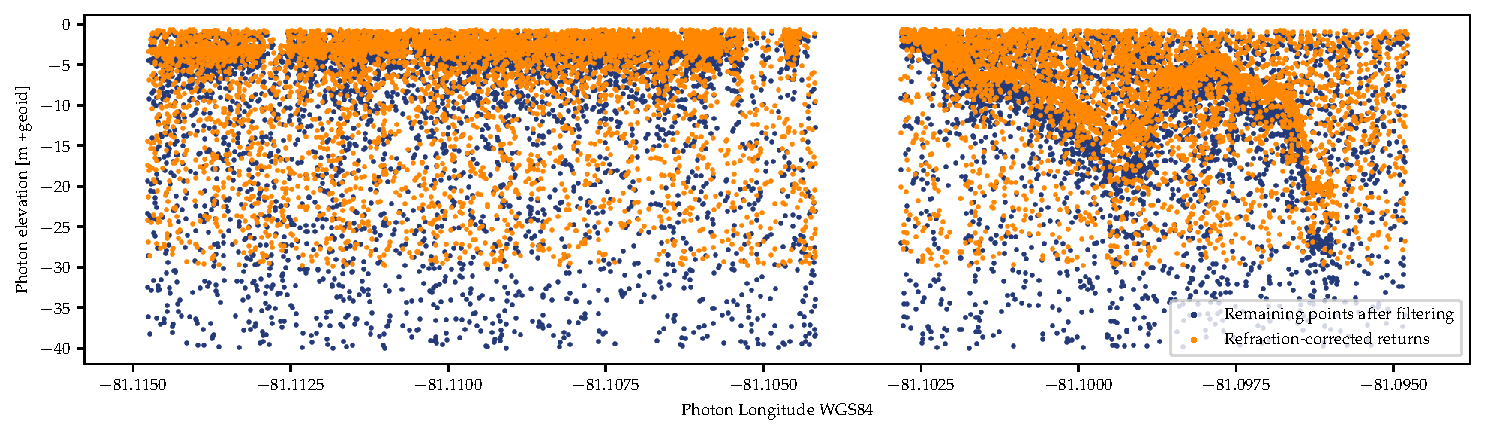
\includegraphics[width=\textwidth]{figures/methodology_refraction.jpg}
    \caption{The refraction correction applied to the remaining photons}
    \label{fig:refraction-photons}
\end{figure}

\subsection{Bathymetric Signal Extraction}\label{sec:kdesignalfinding}

The filtering steps reduce the dataset to just photon that are in the subsurface zone. To determine if there is bathymetric signal present, further processing is required. Some proposed methods for separating bathymetric signal photons from noise are explained in section \ref{subsec:denoising}. For this project\pdfcomment{reword?}, a new method is proposed based on a Gaussian Kernel Density Estimation (KDE) function. A function is created that returns the maximum kernel density, and the Z location at which it occurs. $$ f(\hat{z}_{window}) \rightarrow kde_{max},z_{kde_{max}} $$ Figure \ref{fig:kdefunc} shows the KDE function as applied to an example window, and the resulting kernel density plot. The KDE function is highly influenced by the \emph{Bandwidth} parameter. For this implementation, the Scott method \parencite{Scott2015} is used to estimate the required bandwidth based on the distribution of the data. 

This function is applied on a rolling basis to a window of 100 adjacent photons. This function returns a value for every single point along the transect, including in areas that do not have any noticeable signal. The kernel density value gives an indication of the strength of the peak. To reject the locations where the signal is weak, any points with a KDE value of less than the median value $$ kde_{50} $$ \pdfcomment{maybe just less than median? that decreases RMS error at the florida site} are assigned an NaN value and are dropped from the analysis.

\begin{figure}[htbp]
    \centering
    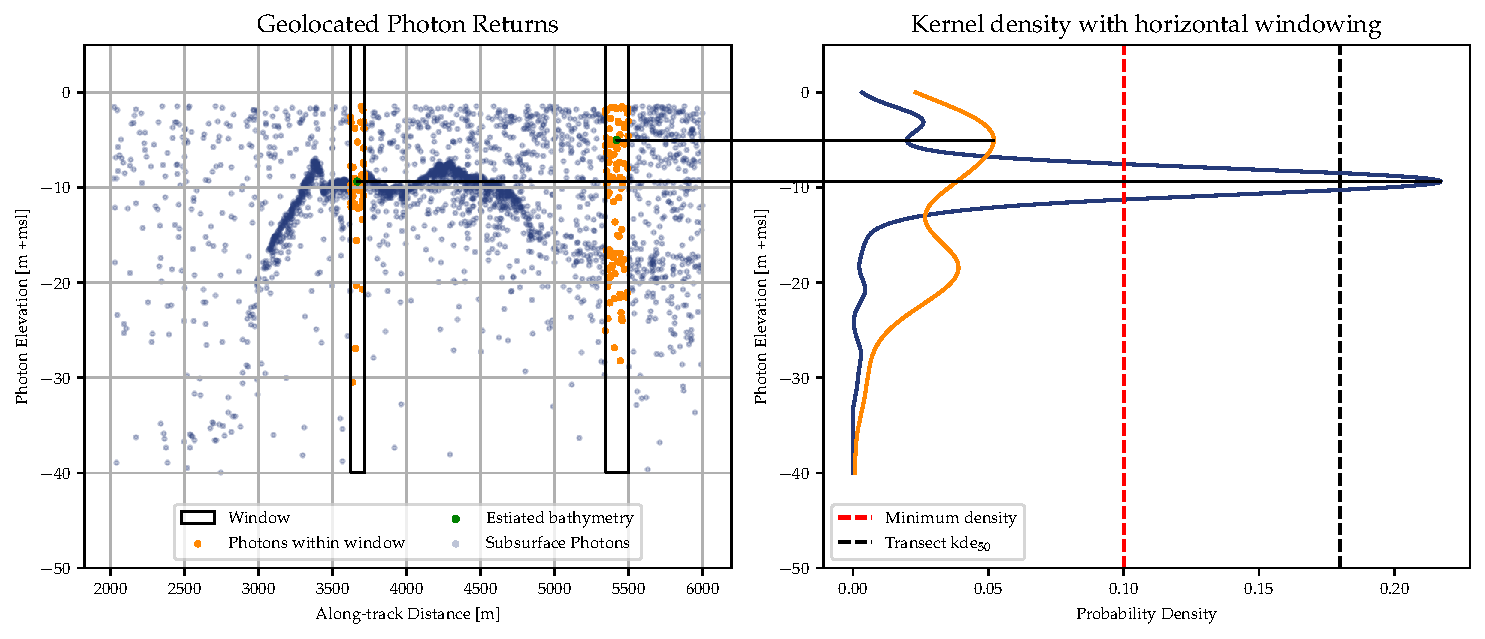
\includegraphics[width=\textwidth]{figures/2d_kde_plot.png}
    \caption{KDE function as applied to single window}
    \label{fig:kdefunc}
\end{figure}

The input parameters to the signal finding function are:

\begin{enumerate}
    \item The size of the window in \emph{number of points}
    \item the cutoff value for the Kernel Density required for point to be considered signal
\end{enumerate}

\subsection{Interpolation to a 2D grid}

After the bathymetric signal points are identified per the method in \ref{sec:kdesignalfinding}, the resulting bathymetry points are densely spaced along satellite tracklines, but are absent between them. A number of interpolation techniques have been applied to create bathymetry grids from point data. Commonly, inverse-distance weighting (IDW), tension splines, or loess interpolators have been used \parencite{gebcocookbook,Ferreira2017,}.

To convert these densely-spaced vector point locations to a raster of elevation data, and a raster of uncertainty data, geostatistical techniques are used.



\subsubsection{Subsampling of Bathymetric points using Poisson Disk Sampling} \label{subsec:poissonsubsampling}
The bathymetric points are extremely densely spaced, and kriging algorithms are computationally expensive. To reduce the number of points fed into the algorithm, a subsample of the points is taken using the poisson disk sampling technique. \pdfmargincomment{Need to expand on this quite a bit}
\pdfcomment{add figure showing points selected vs all points}

\subsubsection{Kriging interpolation}
Using the subsample of the points from the poisson disk sampling, they are converted to a bathymetry raster using Universal Kriging. This geostatistical technique results in both a raster of the estimated depth as well as the estimated uncertainty. 


\subsection{Bayesian Data Assimilation using Kalman Filtering}
The Kalman Filter is a mathematical technique to predict the state of systems based on uncertain measurements. It consist of a loop of two steps, an \emph{Time update} step which updates the position based on a measurement and a known measurement uncertainty, and a \emph{measurement update} step which predicts the state based on the dynamic equations of the system. The kalman filter equations, for a state $x_k$ and a vector of measurements of the state $z_k$:

Time Update:

\begin{equation}
    \hat{x}_{\bar{k}} = A\hat{x}_{k-1} + B\hat{u_{k-1}}
\end{equation}

\begin{equation}
    P_{\bar{k}} = A P_{k-1} A^T + Q
\end{equation}

Measurement Update:
\begin{equation}
    K = P_{\bar{k}} H^T(H P_{\bar{k}} H^T + R) ^{-1}
\end{equation}

\begin{equation}
    \hat{x}_k = \hat{x}_{\bar{k}} + K(\hat{z}_k - H \hat{x}_{\bar{k}})
\end{equation}

\begin{equation}
    P_k = (I - KH)P_{\bar{k}}
\end{equation}


The coastal zone is a highly dynamic system. However, for the purposes of this project is is assumed that the temporal variations over the time scale being studied are within the margin of error of the measurements, so the bathymetry of the nearshore zone is assumed to be a static system and the time update step can be ignored. It is also assumed all measurements are measurements of the same underlying physical depth, and that differences between measurements are due to normally distributed measurement error, with magnitude of the error varying depending on the method. To combine multiple measurements, the \emph{measurement update} step is applied recursively for each available measurement, producing a bayesian estimate of the bathymetry.  

\subsection{Error Evaluation}
\pdfcomment{add RMSE error derivation}
\subsection{Evaluating transect-level variables which predict bathymetry}
\pdfcomment{This could potentially be interesting and also help flesh out my answer to my first research question}
\subsection{Case Studies}
